 % ******************************* PhD Thesis Template **************************
% Please have a look at the README.md file for info on how to use the template

\documentclass[a4paper,12pt,times,numbered,print,custommargin,index,custombib,oneside]{Classes/PhDThesisPSnPDF}
\usepackage{multirow}
\usepackage{comment}
\usepackage{tocloft}
\usepackage{tikz}
\usepackage{wrapfig}
\usepackage{graphicx}
\usepackage{ragged2e}
\usepackage{graphicx} 
\usepackage{capt-of}
\usepackage{float}
\usepackage{lineno}
 \usepackage{setspace}
\usepackage{pgfplots}
\usepackage{booktabs}
\setlength\cftparskip{0pt}
\setlength\cftbeforechapskip{0pt}


% ******************************************************************************
% ******************************* Class Options ********************************
% *********************** See README for more details **************************
% ******************************************************************************

% `a4paper'(The University of Cambridge PhD thesis guidelines recommends a page
% size a4 - default option) or `a5paper': A5 Paper size is also allowed as per
% the Cambridge University Engineering Deparment guidelines for PhD thesis
%
% `11pt' or `12pt'(default): Font Size 10pt is NOT recommended by the University
% guidelines
%
% `oneside' or `twoside'(default): Printing double side (twoside) or single
% side.
%
% `print': Use `print' for print version with appropriate margins and page
% layout. Leaving the options field blank will activate Online version.
%
% `index': For index at the end of the thesis
%
% `draftclassic': For draft mode without loading any images (same as draft in book)
%
% `draft': Special draft mode with line numbers, images, and water mark with
% timestamp and custom text. Position of the text can also be modified.
%
% `abstract': To generate only the title page and abstract page with
% dissertation title and name, to submit to the Student Registry
%
% `chapter`: This option enables only the specified chapter and it's references
%  Useful for review and corrections.
%
% ************************* Custom Page Margins ********************************
%
% `custommargin`: Use `custommargin' in options to activate custom page margins,
% which can be defined in the preamble.tex. Custom margin will override
% print/online margin setup.
%
% *********************** Choosing the Fonts in Class Options ******************
%
% `times' : Times font with math support. (The Cambridge University guidelines
% recommend using times)
%
% `fourier': Utopia Font with Fourier Math font (Font has to be installed)
%            It's a free font.
%
% `customfont': Use `customfont' option in the document class and load the
% package in the preamble.tex
%
% default or leave empty: `Latin Modern' font will be loaded.
%
% ********************** Choosing the Bibliography style ***********************
%
% `authoryear': For author-year citation eg., Krishna (2013)
%
% `numbered': (Default Option) For numbered and sorted citation e.g., [1,5,2]
%
% `custombib': Define your own bibliography style in the `preamble.tex' file.
%              `\RequirePackage[square, sort, numbers, authoryear]{natbib}'.
%              This can be also used to load biblatex instead of natbib
%              (See Preamble)
%
% **************************** Choosing the Page Style *************************
%
% `default (leave empty)': For Page Numbers in Header (Left Even, Right Odd) and
% Chapter Name in Header (Right Even) and Section Name (Left Odd). Blank Footer.
%
% `PageStyleI': Chapter Name next & Page Number on Even Side (Left Even).
% Section Name & Page Number in Header on Odd Side (Right Odd). Footer is empty.
%
% `PageStyleII': Chapter Name on Even Side (Left Even) in Header. Section Number
% and Section Name in Header on Odd Side (Right Odd). Page numbering in footer

% Uncomment to change page style
%\pagestyle{PageStyleII}

% ********************************** Preamble **********************************
% Preamble: Contains packages and user-defined commands and settings
% ******************************************************************************
% ****************************** Custom Margin *********************************

% Add `custommargin' in the document class options to use this section
% Set {innerside margin / outerside margin / topmargin / bottom margin}  and
% other page dimensions
\ifsetCustomMargin
\RequirePackage[left=40mm,right=20mm,top=30mm,bottom=30mm]{geometry}
  \setFancyHdr % To apply fancy header after geometry package is loaded
\fi

% Add spaces between paragraphs
\setlength{\parskip}{0.5em}
% Ragged bottom avoids extra whitespaces between paragraphs
\raggedbottom
% To remove the excess top spacing for enumeration, list and description
%\usepackage{enumitem}
%\setlist[enumerate,itemize,description]{topsep=0em}
\usepackage{bm}
\usepackage{mathtools}
\usepackage{amsmath} 
\usepackage{tikz}
\usepackage{pgfplots}
\usepackage{amsfonts}
\usepackage{amssymb}
\usepackage[makeroom]{cancel}
\usepackage{fancyhdr}
\usepackage{calligra}
\usepackage[bottom]{footmisc}
\usepackage[T1]{fontenc}

\usepackage{tikz}
\def\checkmark{\tikz\fill[scale=0.4](0,.35) -- (.25,0) -- (1,.7) -- (.25,.15) -- cycle;} 
% *****************************************************************************
% ******************* Fonts (like different typewriter fonts etc.)*************

% Add `customfont' in the document class option to use this section

\ifsetCustomFont
  % Set your custom font here and use `customfont' in options. Leave empty to
  % load computer modern font (default LaTeX font).
  %\RequirePackage{helvet}

  % For use with XeLaTeX
  %  \setmainfont[
  %    Path              = ./libertine/opentype/,
  %    Extension         = .otf,
  %    UprightFont = LinLibertine_R,
  %    BoldFont = LinLibertine_RZ, % Linux Libertine O Regular Semibold
  %    ItalicFont = LinLibertine_RI,
  %    BoldItalicFont = LinLibertine_RZI, % Linux Libertine O Regular Semibold Italic
  %  ]
  %  {libertine}
  %  % load font from system font
  %  \newfontfamily\libertinesystemfont{Linux Libertine O}
\fi

\usepackage{tocloft}
% Spacing between lines
\newlength{\toclineskipl}
\setlength{\toclineskipl}{0.5\baselineskip}

% *****************************************************************************
% **************************** Custom Packages ********************************

% ************************* Algorithms and Pseudocode **************************

%\usepackage{algpseudocode}

\usepackage{color}   %May be necessary if you want to color links
\usepackage{hyperref}
%\hypersetup{
%	colorlinks,
%	linktoc=all,
%	citecolor=black,
%	filecolor=black,
%	linkcolor=black,
%	urlcolor=cyan
%}

%\usepackage{url}
%\urlstyle{rm}
% ********************Captions and Hyperreferencing / URL **********************

% Captions: This makes captions of figures use a boldfaced small font.
%\RequirePackage[small,bf]{caption}

\RequirePackage[labelsep=space,tableposition=top]{caption}
\renewcommand{\figurename}{Fig.} %to support older versions of captions.sty


% *************************** Graphics and figures *****************************

%\usepackage{rotating}
%\usepackage{wrapfig}

% Uncomment the following two lines to force Latex to place the figure.
% Use [H] when including graphics. Note 'H' instead of 'h'
%\usepackage{float}
%\restylefloat{figure}
\usepackage{afterpage}
% Subcaption package is also available in the sty folder you can use that by
% uncommenting the following line
% This is for people stuck with older versions of texlive
%\usepackage{sty/caption/subcaption}
\usepackage{subcaption}

% ********************************** Tables ************************************
\usepackage{booktabs} % For professional looking tables
\usepackage{multirow}

\usepackage{multicol}
%\usepackage{longtable}
%\usepackage{tabularx}
%\usepackage[spanish]{babel}

% *********************************** SI Units *********************************
\usepackage{siunitx} % use this package module for SI units


% ******************************* Line Spacing *********************************

% Choose linespacing as appropriate. Default is one-half line spacing as per the
% University guidelines

% \doublespacing
% \onehalfspacing
% \singlespacing

\usepackage{hhline}
% ************************ Formatting / Footnote *******************************

% Don't break enumeration (etc.) across pages in an ugly manner (default 10000)
%\clubpenalty=500
%\widowpenalty=500

%\usepackage[perpage]{footmisc} %Range of footnote options


% *****************************************************************************
% *************************** Bibliography  and References ********************

%\usepackage{cleveref} %Referencing without need to explicitly state fig /table

% Add `custombib' in the document class option to use this section

\ifuseCustomBib
 %\RequirePackage[square, sort, numbers, authoryear]{natbib} % CustomBib

% If you would like to use biblatex for your reference management, as opposed to the default `natbibpackage` pass the option `custombib` in the document class. Comment out the previous line to make sure you don't load the natbib package. Uncomment the following lines and specify the location of references.bib file

\RequirePackage[backend=biber, style=numeric-comp, citestyle=numeric, sorting=nyt, url=false, doi=true, natbib=true]{biblatex}
\addbibresource{References/references} %Location of references.bib only for biblatex, Do not omit the .bib extension from the filename.

\fi

% changes the default name `Bibliography` -> `References'
\renewcommand{\bibname}{References}


% ******************************************************************************
% ************************* User Defined Commands ******************************
% ******************************************************************************

% *********** To change the name of Table of Contents / LOF and LOT ************

%\renewcommand{\contentsname}{My Table of Contents}
%\renewcommand{\listfigurename}{My List of Figures}
%\renewcommand{\listtablename}{My List of Tables}


% ********************** TOC depth and numbering depth *************************

\setcounter{secnumdepth}{2}
\setcounter{tocdepth}{2}


% ******************************* Nomenclature *********************************

% To change the name of the Nomenclature section, uncomment the following line

%\renewcommand{\nomname}{Symbols}


% ********************************* Appendix ***********************************

% The default value of both \appendixtocname and \appendixpagename is `Appendices'. These names can all be changed via:

%\renewcommand{\appendixtocname}{List of appendices}
%\renewcommand{\appendixname}{Appndx}

% *********************** Configure Draft Mode **********************************

% Uncomment to disable figures in `draft'
%\setkeys{Gin}{draft=true}  % set draft to false to enable figures in `draft'

% These options are active only during the draft mode
% Default text is "Draft"
%\SetDraftText{DRAFT}

% Default Watermark location is top. Location (top/bottom)
%\SetDraftWMPosition{bottom}

% Draft Version - default is v1.0
%\SetDraftVersion{v1.1}

% Draft Text grayscale value (should be between 0-black and 1-white)
% Default value is 0.75
%\SetDraftGrayScale{0.8}
%\newenvironment{poliabstract}[1]
%{\renewcommand{\abstractname}{#1}\begin{abstract}}
%	{\end{abstract}}


% ******************************** Todo Notes **********************************
%% Uncomment the following lines to have todonotes.

%\ifsetDraft
%	\usepackage[colorinlistoftodos]{todonotes}
%	\newcommand{\mynote}[1]{\todo[author=kks32,size=\small,inline,color=green!40]{#1}}
%\else
%	\newcommand{\mynote}[1]{}
%	\newcommand{\listoftodos}{}
%\fi
\pgfplotsset{compat=1.16}
% Example todo: \mynote{Hey! I have a note}

% ******************************** Highlighting Changes **********************************
%% Uncomment the following lines to be able to highlight text/modifications.
%\ifsetDraft
%  \usepackage{color, soul}
%  \newcommand{\hlc}[2][yellow]{{\sethlcolor{#1} \hl{#2}}}
%  \newcommand{\hlfix}[2]{\texthl{#1}\todo{#2}}
%\else
%  \newcommand{\hlc}[2]{}
%  \newcommand{\hlfix}[2]{}
%\fi

% Example highlight 1: \hlc{Text to be highlighted}
% Example highlight 2: \hlc[green]{Text to be highlighted in green colour}
% Example highlight 3: \hlfix{Original Text}{Fixed Text}

% *****************************************************************************
% ******************* Better enumeration my MB*************
\usepackage{enumitem}

% ************************ Thesis Information & Meta-data 
% ************************ Thesis Information & Meta-data **********************
% Thesis title and author information, refernce file for biblatex

% ***************************** Abstract Separate ******************************
% To printout only the titlepage and the abstract with the PhD title and the
% author name for submission to the Student Registry, use the `abstract' option in
% the document class.


\ifdefineAbstract
\pagestyle{empty}
\includeonly{Declaration/declaration, Abstract/abstract, Abstract/resumen}
\fi

% ***************************** Chapter Mode ***********************************
% The chapter mode allows user to only print particular chapters with references
% Title, Contents, Frontmatter are disabled by default
% Useful option to review a particular chapter or to send it to supervisior.
% To use choose `chapter' option in the document class

\ifdefineChapter
\includeonly{Chapter3/chapter3}
\fi

% ******************************** Front Matter ********************************
\begin{document}
%	\linenumbers
	\frontmatter
	 %% Aquí comienza el documento.
\thispagestyle{empty} %% PARA QUITAR FORMATO DE PIES Y ENCABEZADOS DE PÁGINA A LA PORTADA
%
%
%
%
%
%
%
%   ESPACIO COMENTADO PARA EVITAR DESAJUSTES POR GENERACIÓN DE NUEVO PÁRRAFO (NO DEJAR ESPACIOS ENTRE MINIPAGES)
%
%
%
%
%
%%%%%%%%% MINIPAGE PARA EL LOGO DEL LADO IZQUIERDO (UNIVERSIDAD) %%%%%%%%%%%%%%%%%%%%%%%%%%%%%%%
%
%
%
%
%\fbox{
\begin{minipage}[c][0.15\textheight][c]{0.25\textwidth}
    \begin{center}
        
\includegraphics[height=3.2cm, keepaspectratio=true]{unison-logo.png} %% LOGO IZQUIERDO
    \end{center}
\end{minipage}
%}
%
%
%
%
%
%
%   ESPACIO COMENTADO PARA EVITAR DESAJUSTES POR GENERACIÓN DE NUEVO PÁRRAFO (NO DEJAR ESPACIOS ENTRE MINIPAGES)
%
%
%
%
%
%%%%%%%%%%%%% MINIPAGE PARA EL CUERPO DE LA PORTADA (NOMBRES, TITULOS, ETC.) %%%%%%%%%%%%%%%%%%%%%%%%%%%%%%5
%
%
%
%
%\fbox{
\begin{minipage}[c][0.17\textheight][t]{0.7\textwidth}
    \begin{center}
        {\scshape\LARGE UNIVERSIDAD DE SONORA} %% NOMBRE DE LA UNIVERSIDAD
        \vspace{.5cm}   %% DEFINE EL ESPACIO ENTRE EL NOMBRE DE LA UNIVERSIDAD Y LA LÍNEA DOBLE
        \hrule height2.5pt  %% DEFINE EL ANCHO DE LA PRIMER LÍNEA
        \vspace{.1cm}    %% DEFINE EL ESPACIO ENTRE LAS DOS LINEAS
        \hrule height1pt  %% DEFINE EL ANCHO DE LA SEGUNDA LINEA (NORMALMENTE ES MAS DELGADA)
        \vspace{.4cm}   %% DEFINE EL ESPACIO ENTRE LA DOBLE LINEA Y EL NOMBRE DE LA DIVISIÓN
        {\scshape \large Divisi\'on de Ciencias Exactas y Naturales}
        {\scshape Departamento de Investigaci\'on en F\'isica} %% NOMBRE DE LA DIVISIÓN
    \end{center}
\end{minipage}
%}
%
%
%
%
%
%   ESPACIO COMENTADO PARA EVITAR DESAJUSTES POR GENERACIÓN DE NUEVO PÁRRAFO (NO DEJAR ESPACIOS ENTRE MINIPAGES)
%
%
%
%
%
%
%   ESPACIO COMENTADO PARA EVITAR DESAJUSTES POR GENERACIÓN DE NUEVO PÁRRAFO (NO DEJAR ESPACIOS ENTRE MINIPAGES)
%
%
%
%
%
%%%%%%%%%%%%%%%%%%%%%%% MINIPAGE PARA EL LOGO DEL LADO DERECHO (DIVISIÓN ACADÉMICA)
%
%
%
%
%\fbox{

%
%
%
%
%
%    ESPACIO COMENTADO PARA EVITAR DESAJUSTES POR GENERACIÓN DE NUEVO PÁRRAFO (NO DEJAR ESPACIOS ENTRE MINIPAGES)
%
%
%
%
%
%
%%%%%%% RENGLÓN DE ABAJO DEJADO INTENCIONALMENTE EN BLANCO PARA GENERAR NUEVO COMIENZO DE PÁRRAFO  %%%%%%

%%%%%%%%%%%%%%%%%%%%%%%%%%%%%%%%%%%%%%%%%%%%%%%%%%%%%%%%%%%%%%%%%%%%%%%%%%%%%%%%%%%%%%%%%%%%%%%%%%%%%%%%%
%
%
%
%
%
%  ESPACIO COMENTADO PARA EVITAR DESAJUSTES POR GENERACIÓN DE NUEVO PÁRRAFO (NO DEJAR ESPACIOS ENTRE MINIPAGES)
%
%
%
%
%
%
%%%%%%%%%%%%%%%% 5TO MINIPAGE PARA EL CUERPO DE LA PORTADA (NOMBRES, TÍTULO, ETC.) %%%%%%%%%%%%%%%%%%%%%%%%%%%%%%%%%%%%%%
%
%
%
%
%\fbox{
\begin{minipage}[l][0.78\textheight][t]{0.1\textwidth}
    \begin{center}
    \hskip0pt
    \vrule width2.5pt height17cm    %% height definde la altura de la linea gruesa
        \hskip1mm
        \vrule width1pt height17cm  %% height define la altura de la linea delgada
        \end{center}
\end{minipage}
%}
%\fbox{
\begin{minipage}[c][0.78\textheight][t]{0.8\textwidth}
      \begin{center}
      \vspace{2cm}
        {\Large \scshape {Measurement of the luminosity in proton-proton collisions at the CMS experiment of the Large Hadron Collider}

        \vspace{3cm}
%\end{minipage}
%\begin{minipage}[c][0.5\textheight][t]{0.5\textwidth}
{ \fontsize{10pt}{12pt}\selectfont
        \makebox[5cm][c]{\textbf{THESIS}}  \\[10pt]
         in partial fulfillment of the
requirements for the degree of:\\[3pt]
        {\textbf{{Doctorado en Ciencias (F\'isica)}}}\\[20pt]
        By:\\[6pt]
        \textbf{  {Ashish Sehrawat}}

        \vspace{1cm}

        { Director}:\\Dr. Jose Feliciano BENITEZ RUBIO \\
        \vspace{2cm}
        %{ Hermosillo, Sonora} \\ \hskip1.25cm  \\ 28 November, 2023 \\
        { Hermosillo, Sonora} \\[1.25cm]
        \mydateformat\today \\
        }
      \end{center}
\end{minipage}
%}

	\begin{dedication}
  \vspace*{-2cm} % Adjust the -2cm to the amount of space you want to move up
%\centering
%\begin{center}
\section*{Acknowledgement}
%\end{center}
\justify{

I wish to express my profound gratitude to all those who have supported and guided me throughout my journey towards completing my PhD thesis in high energy particle physics, with a focus on the CMS experiment at CERN. Their unwavering support, encouragement, and expertise have been indispensable to my success.

Foremost, I extend my deepest appreciation to my esteemed thesis supervisor, Dr. Jose Feliciano Benitez. His exceptional guidance, profound knowledge, and commitment to scientific exploration have profoundly shaped my research endeavors. Delving into the fascinating world of particle physics under his mentorship has been a privilege, and his continuous support has been pivotal at every stage of my thesis. I am immensely grateful for the opportunity to work under his supervision and for the personal and professional growth I have experienced through his invaluable guidance.

My heartfelt gratitude goes to my parents, Omkar Jagtaran Singh and Anita. Their unconditional love, encouragement, and sacrifices have been the bedrock of my academic journey. Their unwavering belief in my abilities and constant support have been my source of strength and motivation, enabling me to overcome challenges and pursue my passion for scientific exploration. Their constant presence and support throughout this demanding academic endeavor are cherished and deeply appreciated.

I also extend my appreciation to my sisters Priya, Monu, Sonu, Reena, and Seema. Their unwavering encouragement, understanding, and motivation have been an immense source of inspiration. Their belief in my abilities and continuous support have been a pillar of strength, urging me to remain focused and resilient even during challenging times.

I am indebted to my friends and colleagues, especially Rohit Gupta and Mohammad Balal, for their valuable insights, stimulating discussions, and enduring support. Their encouragement, camaraderie and intellectual exchanges have been instrumental in shaping both my research and personal growth.

Finally, I would like to thank University of Sonora and CONACYT for providing financial support to my research.

%I would like to thank my wife El\'izabeth for her unconditional support in the challenges I set for myself, without her this would not be possible. To my advisor, Dr. Jos\'e Ben\'itez, for giving me guidance, patience and, above all, the opportunity to work in such a professional team and join the CMS experiment, that was a dream for me. To the University of Sonora and CONACYT for supporting me in completing this important challenge in my professional career.

\end{dedication}

	%% ******************************* Thesis Declaration ***************************

\begin{declaration}

I hereby declare that except where specific reference is made to the work of 
others, the contents of this dissertation are original and have not been 
submitted in whole or in part for consideration for any other degree or 
qualification in this, or any other university. This dissertation is my own 
work and contains nothing which is the outcome of work done in collaboration 
with others, except as specified in the text and Acknowledgements. This 
dissertation contains fewer than 65,000 words including appendices, 
bibliography, footnotes, tables and equations and has fewer than 150 figures.

% Author and date will be inserted automatically from thesis.tex \author \degreedate

\end{declaration}
	\chapter*{Agradecimientos}

En primer lugar, quiero agradecer a mis padres, quienes han sido mi mayor apoyo durante todo este proceso. Nunca se echaron para atrás y siempre estuvieron dispuestos a darme las herramientas y el respaldo necesario para llevar a cabo esta tarea. Quiero que sepan que no tengo ninguna queja ni arrepentimientos; al contrario, estoy profundamente agradecido por todo lo que han hecho por mí. Siempre confiaron en mí, siempre me alentaron a ser mejor y, sobre todo, siempre estuvieron a mi lado. Gracias, de todo corazón.

A mis hermanas, Elizabeth y Cinthya, les agradezco su apoyo incondicional en todo momento. Sus risas, sus abrazos y sus palabras de aliento fueron un impulso constante para seguir adelante. Ustedes siempre me recordaron que tengo la capacidad suficiente para completar este proyecto, incluso en los momentos en los que yo mismo dudaba. Gracias por estar ahí, siempre.

Al Dr. Feliciano Benítez, mi director de tesis, quiero expresarle mi más sincero agradecimiento por su paciencia, dedicación y confianza. Siempre tuvo la disposición y el tiempo para explicarme y guiarme paso a paso en este proyecto. Su apoyo constante fue vital para mí; sin su guía, no habría logrado ni la mitad de lo que hoy he conseguido. Estaré eternamente agradecido por sus palabras y por haberme acompañado en este camino.

A mis amigos y a todas las personas que me rodearon durante este proceso, especialmente a Val y Johana, les doy las gracias por empujarme a seguir adelante y por nunca dejarme solo. Su apoyo incondicional y su compañía fueron un faro en los momentos más complicados. Gracias por creer en mí incluso cuando yo no lo hacía.

Finalmente, y más importante, le doy gracias a Dios. Soy consciente de que esto fue posible porque, en mi debilidad, Él mostró Su fortaleza. Este proyecto, así como mi carrera en general, no hubieran sido posibles sin Su gracia y ayuda constante en mi día a día. A Él le doy toda la gloria y el honor.

	\begin{abstract}
\begin{center}
    {\huge Abstract}
\end{center}


\end{abstract}

	\begin{abstract}
    \begin{center}
    {\huge Resumen}
\end{center}



\end{abstract}

	
	% *********************** Adding TOC and List of Figures ***********************
	
	\tableofcontents
	\pagebreak
	\listoffigures
	\pagebreak
	\listoftables
	\pagebreak
	% \printnomenclature[space] space can be set as 2em between symbol and description
	%\printnomenclature[3em]
	
	\printnomenclature
	
	% ******************************** Main Matter *********************************
	\mainmatter
	
	\chapter{Introduction to collider experiments}  %Title of the First Chapter

\ifpdf
    \graphicspath{{Chapter1/Figs/Raster/}{Chapter1/Figs/PDF/}{Chapter1/Figs/}}
\else
    \graphicspath{{Chapter1/Figs/Vector/}{Chapter1/Figs/}}
\fi

%\section{Introduction to collider experiments}
%\label{sec:introduction}

Collider experiments are a type of particle physics experiment that typically involve high energy collisions of electrons or protons. %colliding particles, typically protons or electrons, at very high energies.
These collisions can lead to the creation of new particles or the detection of new phenomena, providing insight into the fundamental nature of matter. Colliders are designed to accelerate particles to nearly the speed of light and guide them along a circular or linear path using magnetic fields. By colliding particles, physicists can study the resulting particle showers and detect the products of the collision using complex detectors. Two important parameters in the collider experiments are energy and luminosity. Collider experiments have played a crucial role in advancing our understanding of particle physics and continue to be a vital tool for scientific exploration. 

\section{Luminosity and its importance in particle physics}

Luminosity is a measure of the number of particle collisions that occur per unit area per unit time. In particle physics, luminosity is a crucial parameter that determines the rate at which interesting particles may be produced in a collider experiment \cite{Herr:941318}.

The instantaneous luminosity of a collider for head-on collisions is given by the following equation:

\begin{equation}
L_{inst} = \frac{N_1 N_2 f}{A} 
\end{equation}

where $N_1$ and $N_2$ are the number of particles in each beam, $f$ is the frequency of bunch crossings, and $A$ is a parameter that takes into account the overlap between the two beams that is the product of beam size.

The importance of luminosity in particle physics lies in its direct relationship with the production rate of particles of interest. The production rate of a given particle is the product of the luminosity and the cross-section of the process. Thus, luminosity directly affects the ability to detect rare events.
%The more collisions that occur, the higher the probability of rare events happening, such as the creation of new particles or the detection of new phenomena.
Additionally, precise measurements require a large number of collisions to be able to statistically determine the properties of the particles being studied.

The rate (R) of a given particle can be expressed as:

\begin{equation}
R = \sigma \: L_{inst} 
\end{equation}

where %R is the production rate,
$L_{inst}$ is the instantaneous luminosity, and $\sigma$ is the cross-section of the process that produces the particle. The cross-section is a measure of the probability that a given process will occur, and it is typically a very small number, on the order of picobarns ($10^{-36} cm^2$).
In order to achieve high luminosity, particle accelerators use various techniques to increase the number of particles in the beams and focus them to a small cross-sectional area. This is done by using superconducting magnets to guide the particles along a circular path and keep them confined to a small area. Another technique is to use radio frequency cavities to accelerate the particles to higher energies increasing the frequency of bunch crossings. In high-energy particle accelerators, such as the Large Hadron Collider (LHC) at CERN, the integrated luminosity is typically measured in units of inverse femtobarns ($fb^{-1}$), which is a measure of the total number of collisions per unit area during the course of an experiment.
%For example, the LHC has a design luminosity of $10^{34} cm^{-2}s^{-1}$, which means that there are $10^{34}$ proton-proton collisions per square centimeter area per second.
The importance of luminosity can be seen in the many discoveries that have been made in particle physics due to high luminosity experiments. For example, the discovery of the Higgs boson at the LHC was made possible by the high luminosity of the collider, which allowed physicists to observe the rare Higgs boson signal over the background noise of other particles. In addition to discoveries, high luminosity experiments are also important for precision measurements. For example, the precise measurement of the properties of the top quark, the heaviest known elementary particle, benefits significantly from the large number of collisions at the LHC. These collisions provide a robust dataset that reduces the uncertainty in the top quark mass measurement, allowing for more precise determination than were possible at the Tevatron.
%For example, the measurement of the properties of the top quark, the heaviest known elementary particle, requires a large number of collisions to be able to distinguish the signal from the background noise.

\section{Motivation for precision luminosity measurement}

%One important measurement in particle physics is the measurement of the luminosity of the colliding beams. The luminosity is a measure of the number of collisions that are occurring per unit time in unit area. This measurement is important because it provides information about the rate at which rare processes occur, and it is necessary for precise measurements of cross sections and other properties of particles like couplings to fermions and bosons. The luminosity measurement with the pixel detector at the CMS experiment is a crucial measurement for the understanding of the LHC physics. The main motivation for this study is to improve the accuracy of the luminosity measurement, which is essential for many physics analyses, including searches for new particles and measurements of the properties of known particles. Luminosity uncertainty is one of the dominant uncertainty in Higgs Boson cross section and coupling measurement with other gauge bosons and fermions as shown in Fig.~\ref{fig:lum_unc}. Uncertainty in cross section and coupling measurement can not be better than uncertainty in luminosity measurement. 

In particle physics, the luminosity of colliding beams is a crucial measurement as it provides information about the rate at which rare processes occur and enables precise measurements of particle properties such as cross-section and couplings to fermions and bosons. Luminosity depends on several variables, including the number of protons in each beam, the size and shape of the beams, and their relative positioning. A slight change in any of these variables can significantly alter the luminosity.
%which in turn affects the interpretation of collision data.
Therefore, it is crucial to measure the luminosity with high precision.

Precision in luminosity measurement allows for the accurate determination of the Standard Model parameters, such as the masses of fundamental particles and the strength of their interactions (coupling constants). These parameters are critical for making precise predictions about particle behavior in high-energy collisions. By refining these parameters, physicists can enhance their understanding of the universe fundamental structure and forces.
High precision luminosity measurement increase the ability to observe rare processes that occur at very low rates. Such processes might be signatures of new physics beyond the Standard Model, including new particles or forces. Distinguishing these rare events from the background noise is crucial for advancing our understanding of the universe.
The electroweak theory, which unifies the weak nuclear force and electromagnetism, makes precise predictions about the production and decay rates of W and Z bosons. Accurate luminosity measurements are essential for comparing these theoretical predictions with experimental data. Any discrepancies could indicate new physics or the need for adjustments within the Standard Model.
Quantum Chromodynamics (QCD) describes the strong force, one of the four fundamental forces. Experiments that measure jet production rates and other phenomena related to the strong force depend on precise luminosity measurements for validating QCD predictions. This understanding is crucial for both the theoretical framework and for interpreting results of particle collision experiments.
High precision in luminosity measurement allows experimental results to be benchmarked against theoretical models with greater accuracy. This benchmarking is essential for validating or refuting theories about the fundamental constituents and forces of the universe.

%The measurement of luminosity with the pixel detector at the CMS experiment is particularly important  as it is a highly precise detector that is capable of measuring luminosity with great accuracy. It provides information about the number of charged particles passing through the detector, which is directly proportional to the number of collisions. This information is then used to calculate the luminosity. 
Improving the uncertainty in luminosity measurements is essential for many physics analyses.
%including searches for new particles and measurements of the properties of known particles.
It is a dominant factor in the measurement of Higgs Boson cross sections and couplings to other gauge bosons and fermions projected for High luminosity (HL)-LHC era, as shown in Fig~\ref{fig:lum_unc}. As such, the uncertainty in cross-section and coupling measurements cannot be better than the uncertainty in luminosity measurement. Therefore, ongoing efforts are focused on improving the precision of luminosity measurements, with the pixel detector at CMS being a key component of this effort. By reducing the luminosity uncertainty, physicists can make more precise measurements of particle properties and potentially discover new physics beyond the Standard Model.

%In particle physics, the luminosity of colliding beams plays a crucial role as it provides crucial data about the frequency at which rare processes take place. This enables the precise measurement of particle properties such as cross sections and couplings to fermions and bosons. Measuring luminosity with high accuracy is paramount, as it gives information about the number of charged particles that are involved in collisions. This data is then employed to determine the luminosity. Enhancing the precision of luminosity measurements is vital for numerous physics analyses, including the search for new particles and determining the properties of known particles. Luminosity uncertainty is a significant factor in the measurement of Higgs Boson cross sections and its couplings to other gauge bosons and fermions, as depicted in Fig~\ref{fig:lum_unc}. Consequently, the uncertainty in cross-section and coupling measurements cannot surpass the uncertainty in luminosity measurement. For this reason, continuous efforts are being made to increase the accuracy of luminosity measurements. By decreasing the luminosity uncertainty, physicists can achieve more accurate measurements of particle properties and potentially uncover new physics that lies beyond the confines of the Standard Model.

\begin{figure}[!htp]
\centering
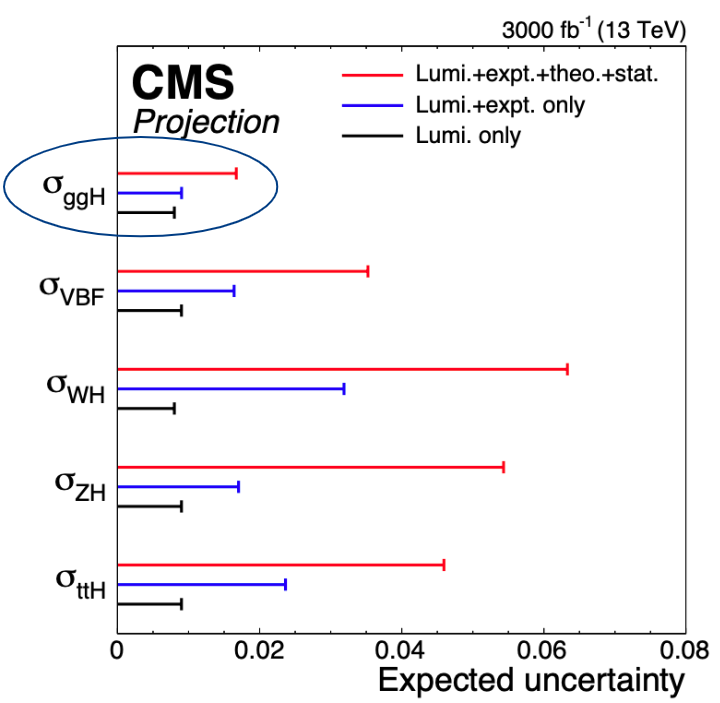
\includegraphics[width=0.8\textwidth]{ashish_thesis/lumi_precision.png}
\caption[Phase 2 uncertainty projection]{ %
   Higgs boson production processes cross section projected uncertainty. In the most precisely measured Higgs boson production process, gluon fusion (ggH), luminosity uncertainty will dominate other experimental systematic uncertainty at the HL-LHC \cite{Dainese:2703572}.
}
\label{fig:lum_unc}
\end{figure}

%\begin{center}
 % \begin{figure}[h]
  %  \centering
   % 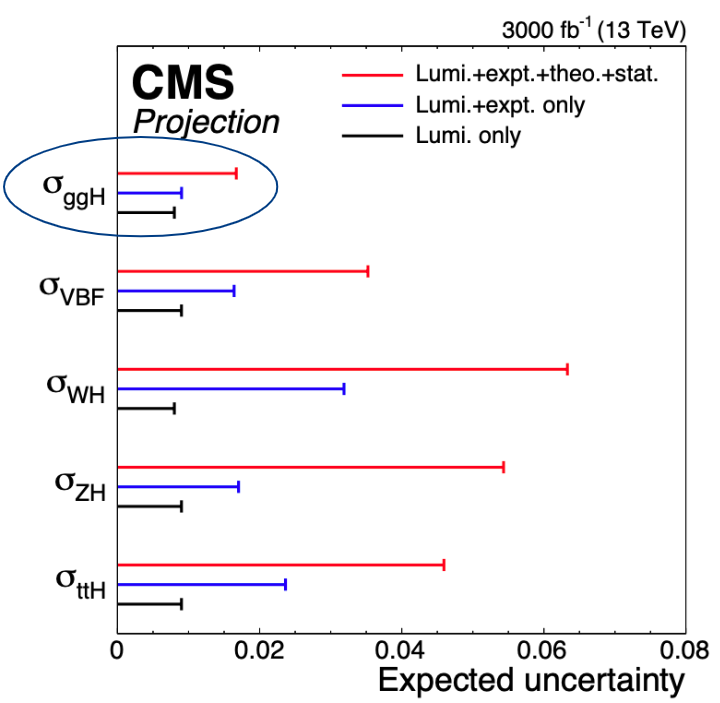
\includegraphics[scale=.35]{ashish_thesis/lumi_precision.png}
    %\caption[Phase II uncertainty projections]{Higgs boson production processes cross section projected uncertainty. In the most precisely measured Higgs boson production process, gluon fusion (ggH), luminosity uncertainty will dominate the experimental systematic uncertainty at the High Luminosity (HL)-LHC.}
    %\label{fig:lum_unc}
  %\end{figure}
%\end{center}

\section{Large Hadron Collider and the CMS Experiment}

The CERN accelerator complex consists of a series of accelerators that work together to produce beams of particles at ever-increasing energies. These beams are then fed into the Large Hadron Collider (LHC) for further acceleration and collision. The first step in the accelerator complex is the Linac 2, a linear accelerator that produces beams of protons with an energy of 50 MeV (mega-electronvolts). The protons are then sent to the Proton Synchrotron Booster (PSB), which accelerates them to an energy of 1.4 GeV (giga-electronvolts). From there, the proton beams are sent to the Proton Synchrotron (PS), which further accelerates them to an energy of 25 GeV. The next step in the complex is the Super Proton Synchrotron (SPS), which accelerates the protons to an energy of 450 GeV. The SPS also produces beams of heavy ions, such as lead nuclei, which are used for experiments in nuclear physics and other fields. Finally, the proton beams are sent to the LHC, where they are accelerated to their maximum energy of 6.5 TeV per proton.

The LHC consists of a 27-kilometer ring of superconducting magnets, which guide two counter-rotating beams of protons to collide at four different locations around the ring, where four major experiments, ATLAS, the Compact Muon Solenoid (CMS) experiment, ALICE and LHCb are located as shown in Fig.~\ref{fig:lhc}. The protons are organized into "bunches," with each bunch containing around 100 billion protons. The bunches are spaced apart by 25 nanoseconds, and the LHC can contain up to 2,808 bunches per beam. The bunches in the LHC are designed to have a beam current of 0.55 amperes. It uses radiofrequency (RF) cavities to accelerate the proton beams. The RF frequency used is 400 MHz, which corresponds to a wavelength of 75 centimeters. The LHC uses quadrupole magnets to focus the proton beams and keep them tightly collimated. The LHC uses a total of 1,232 superconducting dipole magnets to bend the proton beams around the circular accelerator ring. The dipole magnets are cooled to a temperature of 1.9 Kelvin (-271.3°C) using liquid helium, and are capable of producing a magnetic field of up to 8.3 tesla. The LHC's detectors record data from proton-proton collisions at a rate of around 40 million bunch crossings per second, but only a tiny fraction of these are actually recorded for analysis. The LHC operates at a vacuum pressure of around $10^{-13}$ atmospheres, which is lower than the pressure on the surface of the moon.

\begin{figure}[!htp]
\centering
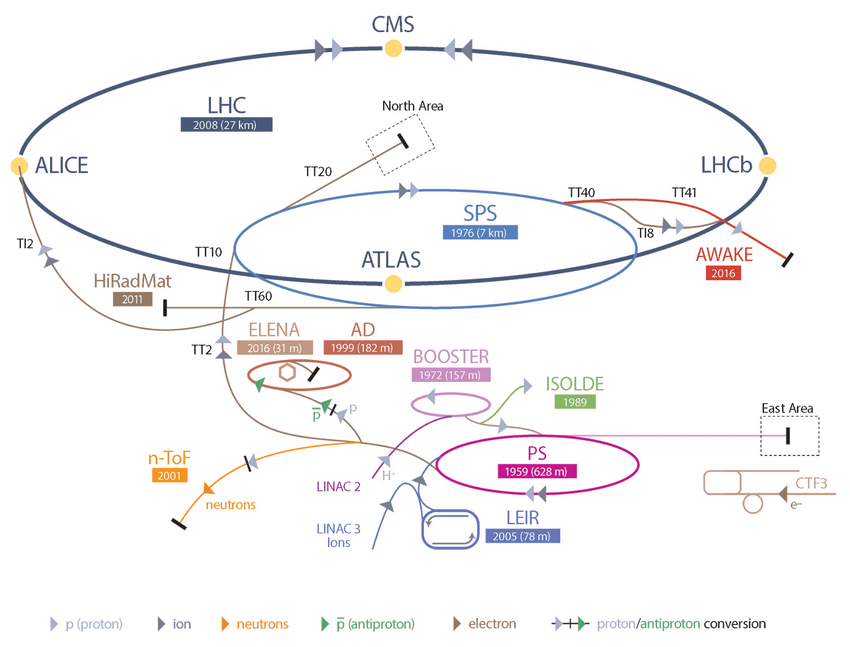
\includegraphics[width=0.9\textwidth]{ashish_thesis/lhc_schematic.png}
\caption[CERN accelerator complex]{%
    CERN accelerator complex consists of Linac 2, Proton Synchrotron Booster (PSB), Proton Synchrotron (PS), Super Proton Synchrotron (SPS) and Large Hadron Collider (LHC) which is the accelerator chain for proton physics at the LHC. LHC ring showing four interaction points where the ALICE, ATLAS, LHCb and CMS detectors are stationed \cite{lhc_complex}.
}
\label{fig:lhc}
\end{figure}

The CMS experiment \cite{CMS:2008xjf} is a multi-purpose particle detector that is designed to detect and study the particles produced in the collisions at the LHC. The CMS detector is a complex instrument that consists of several layers of sub-detectors, each designed to detect different types of particles and measure different properties of the particles. The CMS detector consists of a tracker, an electromagnetic calorimeter, hadron calorimeter, and a muon detector. 

\begin{itemize}

%\item The tracker is a key component of the Compact Muon Solenoid (CMS) detector, located at the Large Hadron Collider (LHC) at CERN. The tracker is responsible for measuring the trajectories of charged particles produced in collisions at the LHC, providing crucial information about the particles' momentum and charge. The CMS tracker consists of two main sub-detectors, the silicon pixel detector and the silicon strip tracker. The silicon pixel detector is the innermost layer of the tracker and is designed to provide precise measurements of the particles' positions. It is composed of millions of tiny silicon pixels, each capable of detecting the passage of a charged particle and measuring its position to within a few microns. The pixel detector consists of four layers and three forward disks. The silicon strip tracker is located outside the pixel detector and is made up of tens of thousands of thin silicon strips. The strips are arranged in layers perpendicular to the beam axis and provide information about the particles' position in the plane perpendicular to their trajectory. Together, the pixel detector and the strip tracker provide a precise measurement of the particles' trajectory, allowing physicists to reconstruct the paths of particles produced in the collision. Pseudorapidity coverage of the tracker is $|\eta| < 2.5$.


%\item The tracker is the innermost subdetector of the CMS detector, consisting of two components: the pixel detector and the strip detector. It is designed to track the trajectories of charged particles produced in proton-proton collisions. The pixel detector has four layers and three forward disks, while the strip detector has ten layers. The key parameters of the tracker include its resolution, which is about 10 microns in the pixel detector and 20-50 microns in the strip detector, and its coverage, which extends up to a pseudorapidity of 2.5.

\item The tracker is a cylindrical detector made up of two main subsystems: the pixel detector and the silicon strip detector \cite{CMS:2021ime}. The pixel detector, the innermost subsystem near the interaction point, is crucial for precise track reconstruction and vertex identification. It includes four barrel layers and two endcap regions with hybrid pixel detector modules. These modules consist of a silicon sensor, segmented into roughly 100x150 $\mu$m² pixels, and readout electronics. When charged particles pass through the sensor, they create electron-hole pairs that induce a current, which is amplified, shaped, and digitized. The upgraded pixel detector used in Run 2 contained over 120 million pixels, ensuring high granularity and hit efficiency. The pixel detector has a 4.8 $\mu$m  and 7.99 $\mu$m  spatial resolution along 100 $\mu$m and 150 $\mu$m pixel pitch respectively \cite{Dragicevic:2262932}. The silicon strip detector surrounding the pixel detector provides extra tracking points for improved track reconstruction. It comprises of the Tracker Inner Barrel and Disks (TIB/TID) and the Tracker Outer Barrel and Endcaps (TOB/TEC). Silicon strip sensors, segmented into strips with a pitch of 80 to 205 $\mu$m, generate electron-hole pairs like the pixel detector. The signals are then processed by the readout electronics.
  %The silicon strip detector has a spatial resolution of 20-30 $\mu$m in the barrel region and 30-45 $\mu$m in the endcap region.

  %The tracker is a cylindrical-shaped detector designed to reconstruct the trajectories of charged particles with high precision. The tracker is composed of two main subsystems: the pixel detector, located closest to the interaction point, and the silicon strip detector, surrounding the pixel detector. The pixel detector is the innermost subsystem of the CMS tracker, providing high-resolution spatial measurements essential for precise track reconstruction and vertex identification. The pixel detector consists of four barrel layers and two endcap regions, each with three disks. The pixel detector is built from hybrid pixel detector modules, which consist of a silicon sensor and readout electronics. The silicon sensor is segmented into an array of individual pixels, each with dimensions of approximately $100 x 150 \mu m^2$. When charged particles traverse the silicon sensor, they create electron-hole pairs, which drift under the influence of an electric field to the nearest pixel electrode, inducing a current. The readout electronics, implemented using custom Application Specific Integrated Circuits (ASICs), amplify, shape, and digitize the signals, enabling precise measurement of the particle's position. During the 2018 data-taking period, the pixel detector employed the upgraded Phase-1 detector, which featured enhanced radiation tolerance and improved readout electronics. The upgraded pixel detector incorporated more than 120 million pixels, providing excellent granularity and high hit efficiency ($>99\%$) for charged particles. the pixel detector has a spatial resolution of approximately 10 $\mu m$ in the local x-coordinate (transverse to the beam direction, azimuthal) and 30 $\mu m$ in the local y-coordinate (vertical to the beam direction, radial). The silicon strip detector surrounds the pixel detector and is responsible for providing additional tracking points to improve the overall track reconstruction efficiency and momentum resolution. The strip detector is divided into two subsystems: the Tracker Inner Barrel and Disks (TIB/TID) and the Tracker Outer Barrel and Endcaps (TOB/TEC). The TIB/TID consists of four barrel layers and three endcap disks on either side of the barrel region. The TOB/TEC has six barrel layers and nine endcap disks on each side. In total, there are ten barrel layers and twelve endcap disks in the strip detector. The silicon strip sensors are segmented into elongated strips, with a pitch ranging from 80 to 205 $\mu m$, depending on the detector region. As charged particles pass through the silicon strip sensors, they generate electron-hole pairs similar to the pixel detector. The induced signals on the strip electrodes are then amplified, shaped, and digitized by the readout electronics. The silicon strip detector offers a spatial resolution of 20-30 $\mu m$ in the barrel region and 30-45 $\mu m$ in the endcap region.

%To cope with the high particle flux and radiation environment, the strip detector employs radiation-hardened sensors and readout electronics. Additionally, an efficient cooling system is used to maintain a stable operating temperature, ensuring consistent performance throughout the data-taking period.

%\item The tracker is a crucial component of the CMS detector, which is located at the LHC at CERN. The tracker is responsible for measuring the trajectories of charged particles produced in collisions at the LHC, providing essential information about the particles' momentum and charge. The CMS tracker consists of two main sub-detectors: the silicon pixel detector and the silicon strip tracker. The silicon pixel detector is the innermost layer of the tracker and is designed to provide precise measurements of the particles' positions. It consists of millions of tiny silicon pixels, each capable of detecting the passage of a charged particle and measuring its position to within a few microns. The pixel detector has four layers arranged around the beam axis and three forward disks located at each end. The forward disks provide coverage at higher pseudorapidity values, where particles are produced at more extreme angles with respect to the beam axis. The silicon strip tracker is located outside the pixel detector and is made up of tens of thousands of thin silicon strips arranged in layers perpendicular to the beam axis. The strips provide information about the particles' position in the plane perpendicular to their trajectory, complementing the precise position measurements provided by the pixel detector. The strip tracker covers a wider area than the pixel detector and has more layers, allowing for more precise measurements of the particles' trajectories. The pseudorapidity coverage of the tracker is $|\eta| < 2.5$. This means that the tracker can measure particles produced at a wide range of angles with respect to the beam axis, up to approximately 75 degrees away from the beamline. The coverage of the tracker is important because it ensures that particles produced at all angles can be detected, providing a complete picture of the collision event.

\item The Electromagnetic Calorimeter (ECAL), a part of the CMS detector, is crucial for measuring the energy of photons and electrons from collisions. The ECAL contains over 75,000 lead tungstate (PbWO4) crystals arranged cylindrically around the interaction point. When photons or electrons hit the crystals, they generate a secondary particle shower, producing scintillation light proportional to the energy of the incoming particle. By assessing this light in each crystal using avalanche photodiodes and vacuum phototriodes \cite{Hobson:2008zz}, the ECAL can precisely determine the energy of the incoming particle. The ECAL covers a pseudorapidity range $|\eta| < 3.0$ \footnote{The pseudorapidity $\eta$ is calculated as $\eta = - \ln(\tan(\frac{\theta}{2}))$ and ranges from $-\infty$ to $+\infty$.}, facilitating measurement of particles at various angles to the beam axis. Its arrangement includes a barrel region and two endcap regions. The PbWO4 crystals vary in size and orientation in these regions to match particle trajectories. They are sufficiently long to absorb incoming particle energy. The ECAL boasts an energy resolution of less than 0.5\% for 50 GeV electrons and less than 1\% for 100 GeV photons. This precision results from the small crystal size, the PbWO4 crystals' high light yield, and advanced calibration procedures. Moreover, it has excellent timing resolution, crucial for differentiating between particles from the same collision and rejecting background events.

  %The Electromagnetic Calorimeter (ECAL) is an important component of the Compact Muon Solenoid (CMS) detector located inside the solenoid magnet of the Compact Muon Solenoid (CMS) detector. Its main function is to measure the energy of photons and electrons that are produced in collisions. The ECAL is made up of more than 75,000 lead tungstate (PbWO4) crystals, arranged in a cylindrical shape around the interaction point. When photons or electrons enter the crystals, they interact with the lead atoms, producing a shower of secondary particles. These particles, in turn, produce scintillation light that is detected by photodetectors at the end of each crystal. The scintillation light produced by the crystals is proportional to the energy of the incoming photon or electron. By measuring the amount of light produced in each crystal, the ECAL is able to determine the energy of the incoming particle with great precision. The ECAL covers the pseudorapidity range $|\eta| < 3.0$, which corresponds to a solid angle of approximately 11,000 square degrees. This ensures that the detector can measure photons and electrons produced at a wide range of angles with respect to the beam axis. The ECAL is arranged in a cylindrical shape around the interaction point, with a barrel region and two endcap regions. The barrel covers the range $|\eta| < 1.479$, while the endcaps cover the range $1.479 < |\eta| < 3.0$. The crystals in the barrel are oriented perpendicular to the beam axis, while those in the endcaps are tilted to match the curvature of the particle trajectories. The PbWO4 crystals in the ECAL have a front face of 22 x 22 $mm^2$ in the barrel region and 28.62 x 28.62 $mm^2$ in the endcaps. The crystals are 230 mm long in the barrel and 220 mm long in the endcaps, allowing for a total of 25.8 radiation lengths of material to absorb the energy of the incoming photons and electrons. The ECAL has an energy resolution of better than 0.5\% for electrons with energies of 50 GeV, and better than 1\% for photons with energies of 100 GeV. This high precision is achieved through a combination of the small crystal size, high light yield of the PbWO4 crystals, and sophisticated calibration procedures. The ECAL also has excellent timing resolution, with a precision of better than 100 picoseconds for most particles. This is important for distinguishing between particles produced in the same collision event, as well as for rejecting background events.

%\item Electromagnetic Calorimeter (ECAL) is designed to measure the energy of electrons and photons produced in proton-proton collisions. It is made up of lead tungstate crystals and has a coverage of up to a pseudorapidity of 3. The key parameters of the ECAL include its energy resolution, which is about 0.5\% for electrons with energies of 100 GeV, and its granularity, which is about 0.0174 in pseudorapidity and 0.0174 radians in phi.

\item The Hadron Calorimeter (HCAL) \cite{Isik:2810162} in the CMS detector, positioned outside of the Electromagnetic Calorimeter (ECAL), measures the energy of hadrons—particles comprised of quarks bound by the strong nuclear force. Since hadrons are abundantly produced in high-energy LHC collisions, the HCAL design focuses on absorbing their energy for measurement. It is composed of alternating layers of brass, for energy absorption, and plastic scintillator, for light emission when particles pass through for the barrel and endcap calorimeters. HF uses quartz fibers and steel as active and passive components, respectively. Photodetectors convert this light into a measurable electrical signal. The Barrel HCAL, also known as HB in CMS, is the main part of the HCAL that is centered around the beam pipe and extends outwards. The pseudorapidity range for this section of the calorimeter is $|\eta|$ < 1.3. The Endcap HCAL, or HE, is designed to capture particles emitted at larger angles from the beam pipe, extending the coverage of the barrel region. The pseudorapidity range of the Endcap HCAL is 1.3 < $|\eta|$ < 3.0. The Forward HCAL, or HF, is situated at both ends of the detector to capture particles produced at the smallest angles to the beam direction. The pseudorapidity range of the Forward HCAL in the CMS experiment is 3.0 < $|\eta|$ < 5.2.

  %The HCAL, divided into a central barrel region and endcap regions, ensures coverage for particles produced at angles up to $|\eta| < 5.2$, accommodating a broad range of angles and energies up to several hundred GeV.

  %The Hadron Calorimeter (HCAL) is a crucial component of the Compact Muon Solenoid (CMS) detector, located outside of the Electromagnetic Calorimeter (ECAL). The HCAL is responsible for measuring the energy of hadrons, which are particles made up of quarks bound together by the strong nuclear force. Hadrons are produced in abundance in high-energy collisions at the LHC and can carry significant amounts of energy. The HCAL is designed to measure the energy of hadrons by absorbing their energy as they pass through the calorimeter. The HCAL is made up of alternating layers of brass, a dense material that absorbs the energy of hadrons, and plastic scintillator, which emits light when particles pass through it. The light emitted by the plastic scintillator is detected by photodetectors, which convert the light into an electrical signal that can be measured. The HCAL is divided into four sections: the barrel region, which covers the central part of the detector, and the endcap regions, which cover the forward and backward directions. The barrel region is divided into 36 wedges, each of which contains alternating layers of brass and plastic scintillator. The endcap regions consist of brass and plastic scintillator layers arranged in a cylindrical shape around the beam axis. The HCAL provides coverage for particles produced at angles up to $|\eta| < 5.2$. This ensures that the HCAL can detect hadrons produced at a wide range of angles with respect to the beam axis. The HCAL also provides coverage for particles with a wide range of energies, up to several hundred GeV.

%\item Hadron Calorimeter (HCAL) is designed to measure the energy of hadrons produced in proton-proton collisions. It is made up of alternating layers of brass and scintillator and has a coverage of up to a pseudorapidity of 5. The key parameters of the HCAL include its energy resolution, which is about 10\% for hadrons with energies of 100 GeV, and its granularity, which is about 0.087 in pseudorapidity and 0.087 radians in phi.

\item The Muon Chambers \cite{CMS:2018rym} are a vital part of the CMS detector. Designed to detect a variety of particles from high-energy collisions, the CMS is particularly equipped for detecting muons, highly penetrative charged particles that often evade other detection methods. Positioned on the outermost layer of the CMS detector, the muon chambers comprise three types of detectors: drift tubes (DTs), cathode strip chambers (CSCs), and resistive plate chambers (RPCs). The DTs are centrally located in the barrel region, while CSCs cover the forward and backward endcap regions. The RPCs, offering a quick trigger signal for muon detection, are found in both the barrel and endcap regions. These chambers detect muons by observing the ionization when a muon travels through the detector gas. By tracking muon trajectories, scientists can investigate the properties of these particles and explore physics beyond the Standard Model.

  %The Muon Chambers are an essential component of the Compact Muon Solenoid (CMS) detector, which is one of the four main particle detectors at the Large Hadron Collider (LHC) at CERN. The CMS detector is designed to detect a wide range of particles produced in high-energy collisions at the LHC, including muons, which are charged particles that pass through most materials easily and are difficult to detect using other methods. The muon chambers are located on the outermost layer of the CMS detector and are designed to detect muons as they pass through the detector. The muon chambers consist of three types of detectors: drift tubes (DTs), cathode strip chambers (CSCs), and resistive plate chambers (RPCs). The DTs are located in the barrel region, which covers the central part of the detector, while the CSCs are located in the endcap regions, which cover the forward and backward directions. The RPCs are also located in the barrel and endcap regions and are used to provide a fast trigger signal for muon detection. The muon chambers are positioned on the outermost layer of the CMS detector because muons are highly penetrating particles that can pass through many layers of material without interacting. The muon chambers detect muons by measuring the ionization produced when a muon passes through the gas in the detectors. By measuring the trajectories of muons as they pass through the CMS detector, physicists can study the properties of these particles and search for new physics beyond the Standard Model.

%\item The muon chambers are designed to detect muons produced in proton-proton collisions. They are located outside the solenoid and consist of three types of detectors: drift tubes (DTs), cathode strip chambers (CSCs), and resistive plate chambers (RPCs). The key parameters of the muon chambers include their spatial resolution, which is about 100-300 microns in the DTs and CSCs and 1-2 cm in the RPCs, and their coverage, which extends up to a pseudorapidity of 2.4.

\item The CMS experiment employs a powerful superconducting solenoid magnet, composed of niobium-titanium (NbTi) wire, to generate a strong, uniform magnetic field crucial for detecting and measuring charged particles from high-energy collisions. The wire, cooled to -268.5°C with liquid helium, becomes superconducting, carrying substantial electrical currents without heat generation. The cylindrical magnet, among the largest of its kind at 13 meters long and 6 meters in diameter, produces a 3.8 Tesla magnetic field—approximately 100,000 times stronger than Earth's magnetic field. This field bends the trajectories of charged particles as shown in Fig.~\ref{fig:cms}, facilitating momentum measurement and aiding physicists in studying the properties of various particles.
  %such as the 2012-discovered Higgs boson. In conjunction with other CMS detector components, the solenoid magnet enables comprehensive reconstruction of particle properties.

  %The Compact Muon Solenoid (CMS) experiment  uses a powerful superconducting solenoid magnet to produce a strong and uniform magnetic field, which is essential for detecting and measuring the properties of charged particles produced in high-energy collisions. The CMS solenoid magnet is made of niobium-titanium (NbTi) superconducting wire, which is cooled to a temperature of -268.5°C using liquid helium. This low temperature allows the wire to become superconducting, which means it has zero electrical resistance and can carry large electrical currents without generating heat. The magnet is shaped like a cylinder and is 13 meters long and 6 meters in diameter, making it one of the largest solenoid magnets ever constructed. The solenoid magnet generates a magnetic field of 3.8 Tesla, which is about 100,000 times stronger than the Earth's magnetic field. The magnetic field is used to bend the trajectories of charged particles produced in high-energy collisions, allowing their momentum to be measured as shown in Fig.~\ref{fig:cms}. By measuring the momentum and charge of these particles, physicists can identify and study the properties of various particles, such as the Higgs boson, which was discovered in 2012 using the CMS detector. The combination of the solenoid magnet with other components of the CMS detector, such as the tracker, the calorimeters, and the muon chambers, enables physicists to reconstruct the properties of particles produced in collisions.

%The magnet is a superconducting solenoid that produces a magnetic field of 3.8 Tesla. It is designed to bend the trajectories of charged particles produced in proton-proton collisions, allowing for their momentum to be measured as shown in Fig.~\ref{fig:cms}.

\end{itemize}

\begin{figure}[!htp]
\centering
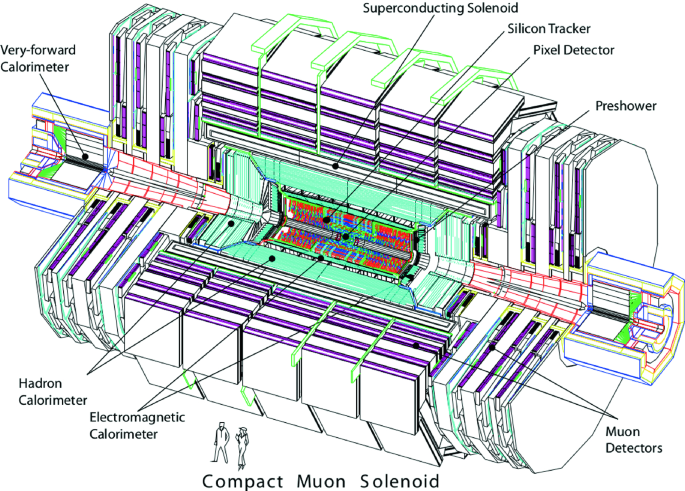
\includegraphics[width=0.75\textwidth]{ashish_thesis/cms_exp.png}
\caption[CMS experiment design]{%
   CMS detector with all of the sub detectors showing silicon tracker, electromagnetic and hadron calorimeters and muon chambers \cite{CMS:2008xjf}. 
}
\label{fig:cms}
\end{figure}


%In summary, luminosity is a critical parameter in particle physics experiments that determines the rate at which particles are produced and detected. The higher the luminosity, the greater the probability of detecting rare or low-probability events. The production rate of a particle of interest is proportional to the product of the luminosity and the cross-section of the process that produces the particle, and increasing the luminosity is essential for increasing the production rate of rare particles.Luminosity is a fundamental concept in particle physics that describes the rate at which particles collide in a particle accelerator. It is defined as the number of particles per unit time and unit cross-sectional area of the particle beams. In other words, it is a measure of the intensity of the particle beams and determines the number of collisions that occur within a given time. The importance of luminosity in particle physics lies in the fact that it directly affects the ability to detect rare events and make precise measurements. The more collisions that occur, the higher the probability of rare events happening, such as the creation of new particles or the detection of new phenomena. Additionally, precise measurements require a large number of collisions to be able to statistically determine the properties of the particles being studied. In high-energy particle accelerators, such as the Large Hadron Collider (LHC) at CERN, the luminosity is typically measured in units of inverse femtobarns ($fb^{-1}$), which is a measure of the total number of collisions per unit area during the course of an experiment. For example, the LHC has a design luminosity of $10^{34} cm^{-2}s^{-1}$, which means that there are $10^{34}$ proton-proton collisions per second per square centimeter of the detector. In order to achieve high luminosity, particle accelerators use various techniques to increase the number of particles in the beams and focus them to a small cross-sectional area. One technique is to use superconducting magnets to guide the particles along a circular path and keep them confined to a small area. Another technique is to use radio frequency cavities to accelerate the particles to higher energies. The importance of luminosity can be seen in the many discoveries that have been made in particle physics due to high-luminosity experiments. For example, the discovery of the Higgs boson at the LHC was made possible by the high luminosity of the collider, which allowed physicists to observe the rare Higgs boson signal over the background noise of other particles. In addition to discoveries, high luminosity experiments are also important for precision measurements. For example, the measurement of the properties of the top quark, the heaviest known elementary particle, requires a large number of collisions to be able to distinguish the signal from the background noise.


\section{Run 1, Run 2 and Run 3 luminosity measurement}

%During the operation of the CMS experiment, two main data-taking periods were conducted: Run 1, which spanned from 2010 to 2013, and Run 2, which took place from 2015 to 2018.
Since the beginning of the operation of the CMS experiment, three main data-taking periods have taken place: Run 1, Run 2, and Run 3, with the latter starting in 2022 and currently ongoing. During these periods, the CMS experiment measured the instantaneous and integrated luminosity of the proton-proton collisions produced by the LHC where the integrated luminosity for each year is shown in Fig.~\ref{fig:lumi}. During Run 1, the CMS experiment achieved a peak instantaneous luminosity of up to $7.6 \times 10^{33} cm^{-2} s^{-1}$, while during Run 2, the luminosity reached a peak value of up to $2.1 \times 10^{34} cm^{-2} s^{-1}$. The luminosity measurements during both runs were accompanied by careful assessments of the systematic uncertainties to ensure accurate and reliable results \cite{CMS-PAS-EWK-10-004, CMS-PAS-EWK-11-001, CMS-PAS-SMP-12-008, CMS-PAS-LUM-13-001, Sirunyan:2759951, pas_17, pas_18} as shown in Table. \ref{tab:lumi}. Luminosity systematic uncertaintities for heavy ion runs is shown in Table \ref{tab:lumi40}.

%\begin{tabular}{c c c c}
%Year & Center of Mass Energy (TeV) & Integrated Luminosity (fb$^{-1}$) & Systematic Uncertainty (\%) \\
%\hline
%2010 & 7 & 0.04 & N/A \\
%2011 & 7 and 8 & 5.6 & 4.5 \\
%2012 & 8 & 23.3 & 2.5 \\
%2015 & 13 & 3.8 & 2.3 \\
%2016 & 13 & 40.8 & 2.5 \\
%2017 & 13 & 49.8 & 2.3 \\
%2018 & 13 & 67.9 & 2.5 \\
%\end{tabular}

\begin{table}[h]
  \centering
  \caption[Integrated luminosity and its precision per year]{Summary of center of mass energy, integrated luminosity, and systematic uncertainty per year in CMS.}
\begin{tabular}{c c c c}
  Year & Center of Mass Energy & Integrated Luminosity & Systematic Uncertainty \\
  & (TeV) & (fb$^{-1}$) & (\%) \\
\hline
2010 & 7 & 0.045 & 11 \\
2011 & 7 and 8 & 6.1 & 2.2 \\
2012 & 8 & 23.3 & 2.5 \\
2015 & 13 & 4.3 & 1.6 \\
2016 & 13 & 41.6 & 1.2 \\
2017 & 13 & 49.8 & 2.3 \\
2018 & 13 & 67.9 &  2.5\\
\end{tabular}
\label{tab:lumi}
\end{table}


\begin{figure}[!htp]
\centering
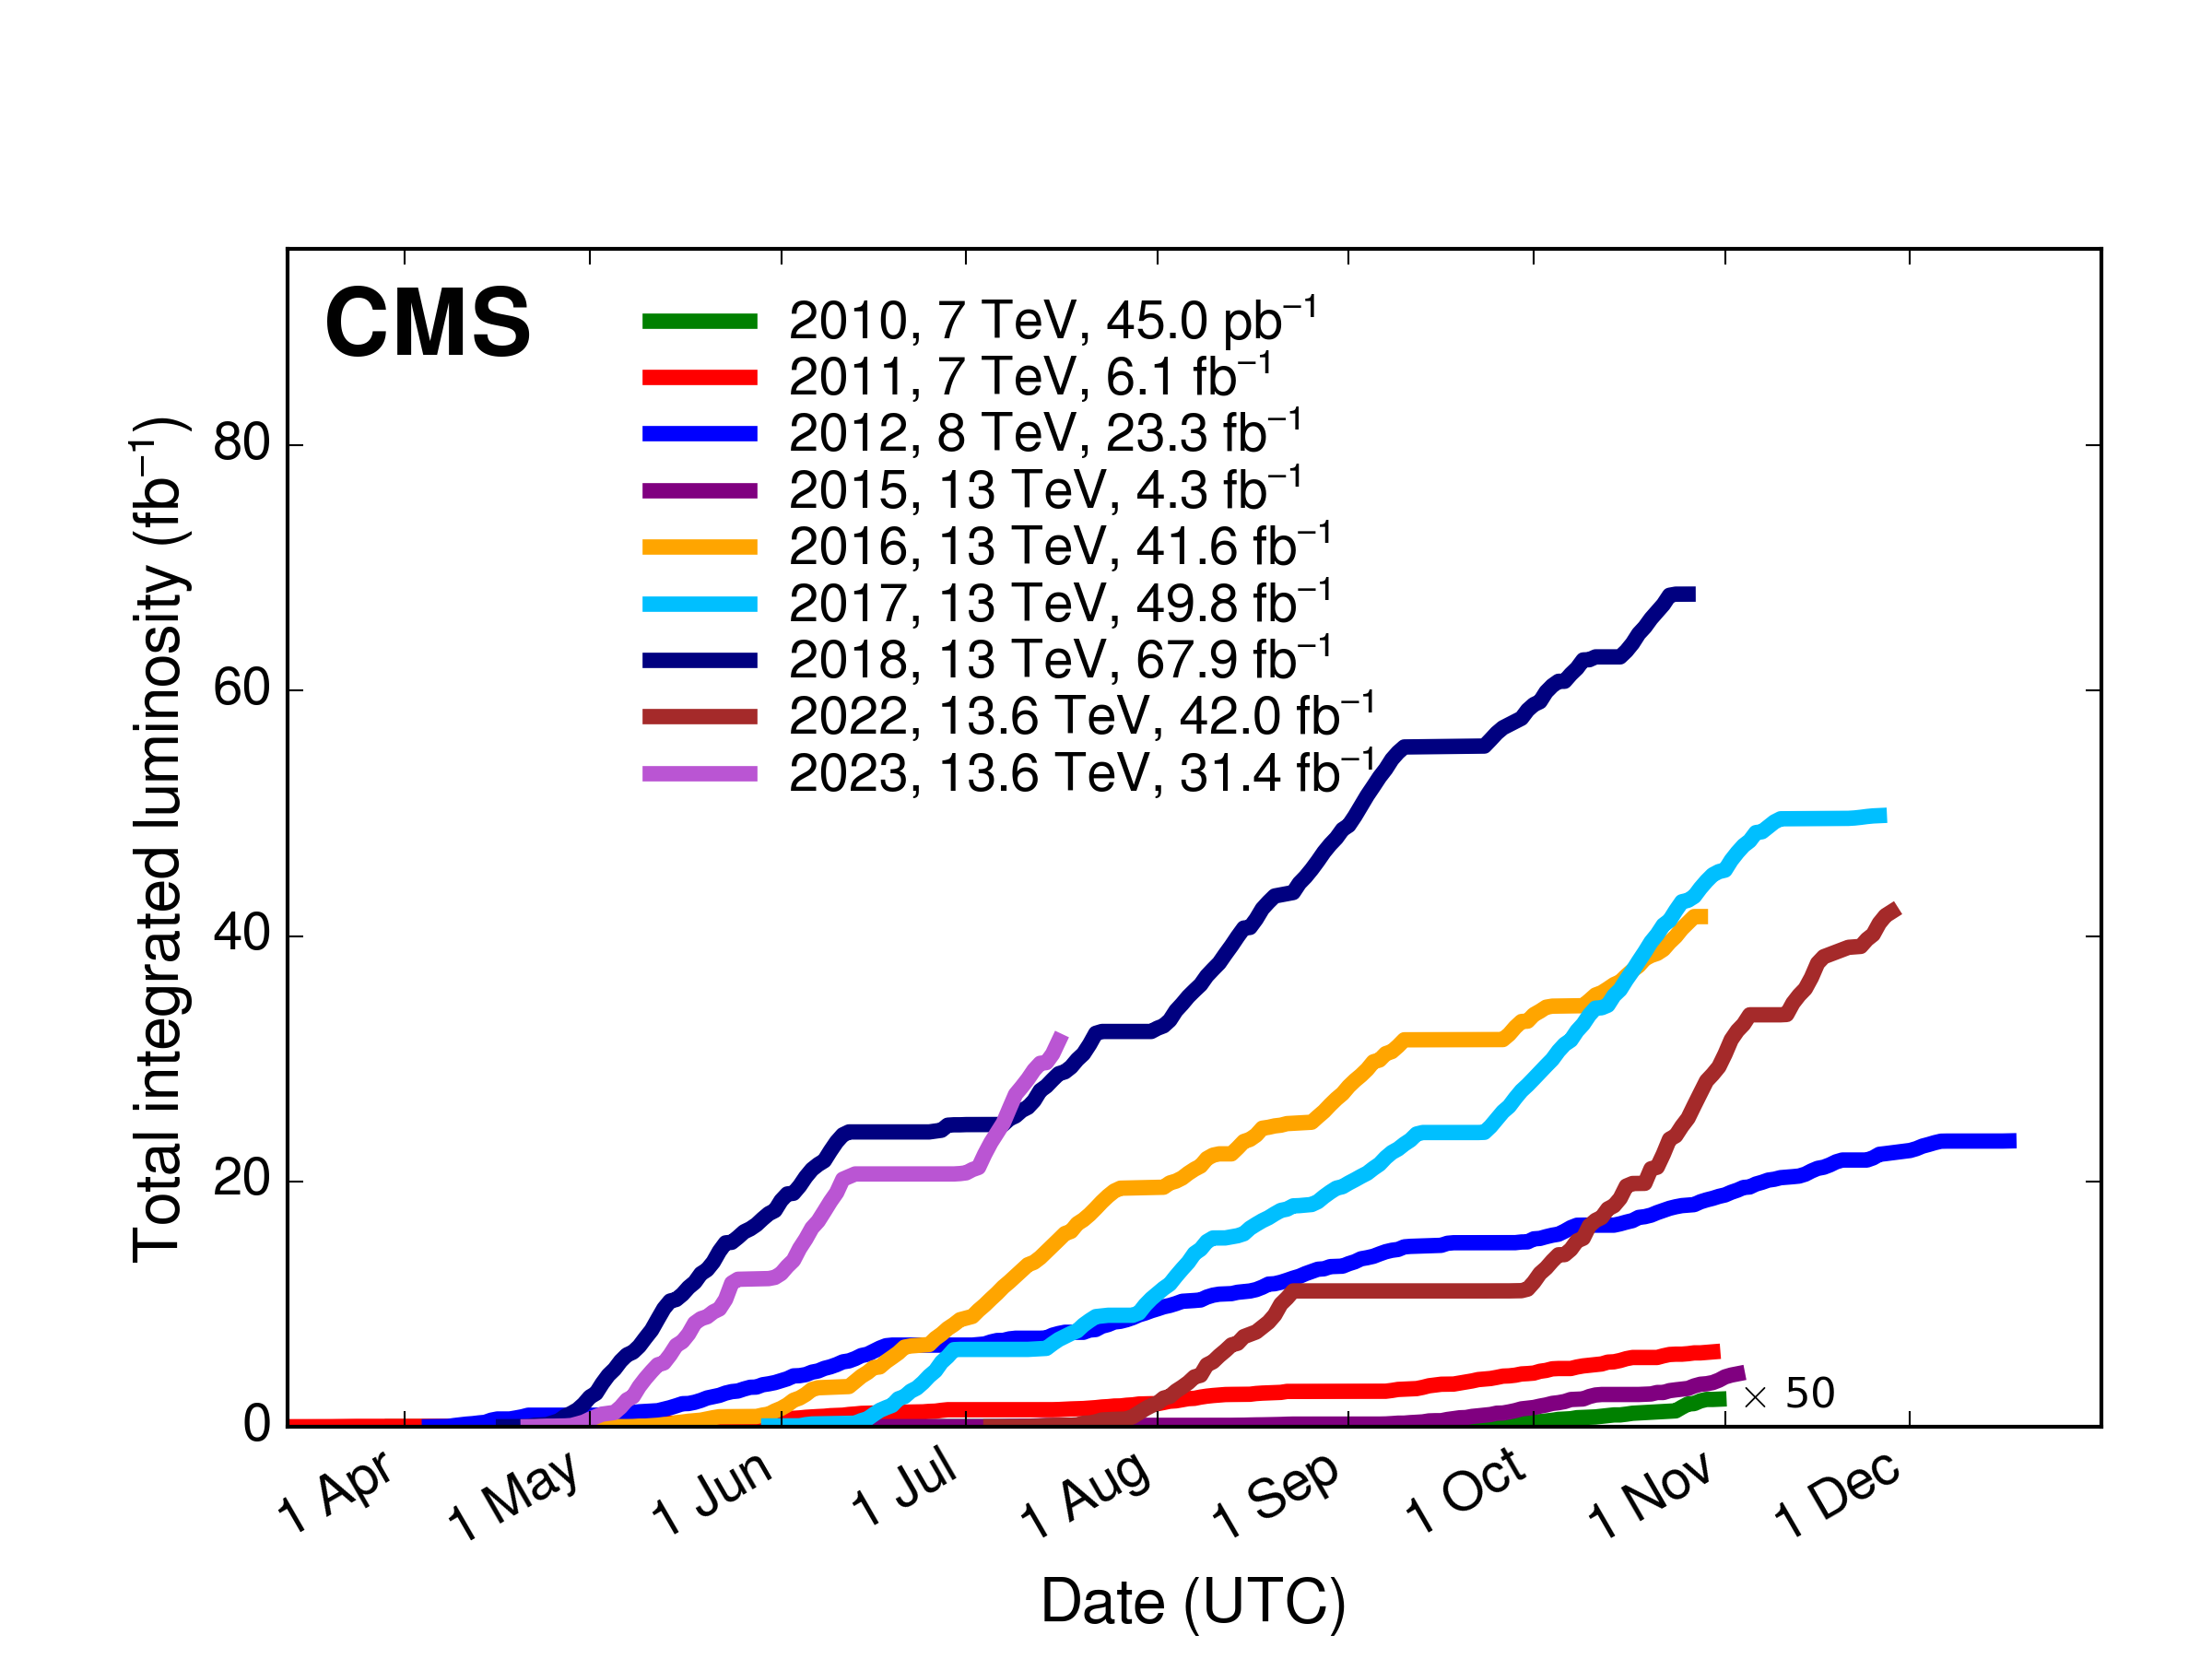
\includegraphics[width=0.9\textwidth]{ashish_thesis/CMS_luminosity.png}
\caption[CMS integrated luminosity]{%
    Delivered luminosity versus time for Run 1, Run 2 and Run 3 of the CMS Experiment \cite{wikicern_cc}.
}
\label{fig:lumi}
\end{figure}


\begin{table}[h]
  \centering
  \caption[Precision for pPb and PbPb collisions]{Summary of center of mass energy and systematic uncertainty per year during the CMS pPb and PbPb luminosity measurement \cite{CMS-PAS-LUM-13-002, CMS-PAS-LUM-17-002, CMS-PAS-LUM-18-001}.}
\begin{tabular}{c c c c}
  Year & Center of Mass Energy/nucleon & Systematic Uncertainty \\
  & (TeV) & (\%) \\
\hline
2013 & 2.76 & 3.4(3.6)  \\
2016 &  5.02  & 3.2(3.7)\\
2018 & 5.02 & 1.5 \\
\end{tabular}
\label{tab:lumi40}
\end{table}


	\chapter{Luminosity measurement at CMS experiment}  %Title of the First Chapter

\ifpdf
    \graphicspath{{Chapter2/Figs/Raster/}{Chapter2/Figs/PDF/}{Chapter2/Figs/}}
\else
    \graphicspath{{Chapter2/Figs/Vector/}{Chapter2/Figs/}}
\fi

%\section{Luminosity measurement at CMS experiment}
%\label{sec:luminositycms}

%Luminosity measurement is a crucial aspect of particle physics experiments such as the Compact Muon Solenoid (CMS) experiment at the Large Hadron Collider (LHC). Luminosity refers to the rate at which particles collide within the detector, and accurate measurement of luminosity is essential for precise determination of particle collision rates and cross-sections. The CMS experiment uses several different devices to measure luminosity, including the Pixel Luminosity Telescope (PLT), Fast Beam Condition Monitor (BCM1F), Hadron forward (HF), Drift tubes (DT), radiation monitoring system for environment and safety (RAMSES) as shown in Fig.~\ref{fig:lumino_cms}. The DT luminometer covers the pseudorapidity range from 0 to 1.2, which is the central region of the CMS detector. The PCC luminometer covers the pseudorapidity range from 0 to 2.5, which covers the central and forward regions of the CMS detector. The HF luminometer covers the pseudorapidity range from 3 to 5, which is the most forward region of the CMS detector. The BCM1F luminometer covers the pseudorapidity range from 3.1 to 4.7, which is also in the forward region of the detector. The RAMSES luminometer covers the pseudorapidity range from 4 to 5, which is also in the forward region of the detector. The PLT luminometer covers the pseudorapidity range from 2.8 to 4.7, which is in the forward region of the CMS detector as shown in Fig.~\ref{fig:lumino_cms_pseudo}. In addition, the Pixel Cluster Counting (PCC) and zero counting method are a commonly used techniques for luminosity measurement at the CMS experiment.

Luminosity measurement is a crucial aspect of particle physics experiments such as the Compact Muon Solenoid (CMS) at the Large Hadron Collider (LHC). Luminosity signifies the rate at which particles collide per unit area per second, making its precision measurement vital for the precise determination of particle collision rates and cross-sections. The CMS experiment employs several devices to measure luminosity, each covering specific pseudorapidity ranges and regions within the CMS detector \cite{CMS-PAS-LUM-18-002}. The use of several luminometers as shown in Fig.~\ref{fig:lumino_cms} offers a multitude of advantages. Primarily, it ensures redundancy and acts as a backup for potential device failures, ensuring that data collection can proceed without interruption. Additionally, having multiple luminometers allows for cross-checking, providing greater consistency in results and allowing for more reliable data interpretation. These different devices enable better control over systematic uncertainties, as any discrepancies can be identified and adjusted for. Moreover, each device employs different method to measure luminosity, providing complementary information that enriches the overall understanding of particle interactions. Some luminometers recording low rates can be calibrated using others, enhancing their accuracy and utility. This holistic approach to luminosity measurement significantly improves the robustness and reliability of the data collected. In the central region, The Muon Drift Tubes (DT) luminometer is used covering a pseudorapidity range from 0 to 1.2. The Pixel Cluster Counting (PCC) luminometer also operates in this region and extends into the forward region covering a range from 0 to 2.5. In the forward region, several devices are utilized. The Pixel Luminosity Telescope (PLT) covers the pseudorapidity range from 2.8 to 4.7. The Fast Beam Condition Monitor (BCM1F) functions in a range from 3.1 to 4.7. The Radiation Monitoring System for Environment and Safety (RAMSES) operates in the pseudorapidity range from 4 to 5. In the most Forward Region, The Hadron forward (HF) luminometer caters to the most forward region of the CMS detector \cite{Sirunyan:2759951}, functioning in the pseudorapidity range from 3 to 5  as shown in Fig.~\ref{fig:lumino_cms_pseudo}.

%In addition to these devices, two common techniques used for luminosity measurement at the CMS experiment are the Pixel Cluster Counting (PCC) and zero counting method. Please refer to Figures 1.1 and 1.2 for further visual information about these devices and their respective coverage within the CMS detector.

\section{Luminosity measurement methods}

%\subsubsection{Luminosity measurement devices at the CMS Experiment}

\begin{itemize}

%\item Pixel Luminosity Telescope (PLT) : The PLT consists of six planes of silicon pixel sensors, which are placed around the beam pipe, covering a total of 13.6 meters in length. Each sensor is divided into many small pixels, which are sensitive to charged particles passing through them. The sensors are positioned at a distance of about 2 mm from the beam center and measure the number of particles that pass through them. Silicon pixel sensors are divided into pixels of size 100 $\times$ 150 $\mu m^2$. The sensors have a thickness of 285 µm and are designed to operate at high radiation levels. PLT's luminosity measurement is to count the number of particles produced in the proton-proton collisions that pass through the silicon pixel sensors. The more particles that pass through the sensors, the higher the luminosity of the collisions. When a proton-proton collision occurs, it produces a shower of particles that pass through the sensors, creating a "hit" in each sensor. The PLT then uses the number of hits recorded by each sensor to determine the luminosity of the collisions.

\item Pixel Luminosity Telescope (PLT) : The PLT consists of four layers of silicon pixel sensors arranged in a stack, with each layer containing over 8 million individual pixels. The first three layers are located very close to the interaction point where the proton beams collide, and the fourth layer is located further away. The innermost layer is located 2.9 cm from the interaction point. The second layer is located 3.9 cm from the interaction point. The third layer is located 4.9 cm from the interaction point. The outermost layer is located 10.2 cm from the interaction point \cite{Ayala:2861814}. The pixel sensors are designed to detect charged particles produced in the collisions as they pass through the detector layers. The PLT operates in what is called the "fast-OR" mode, which detects charged particles produced in a single bunch crossing of the proton beams. In this mode, the PLT triggers on any pixel in the detector that registers a signal above a certain threshold. This signal is called the "fast-OR signal" and indicates that a charged particle has passed through the detector. The PLT uses the information from all four detector planes to reconstruct the trajectories of the charged particles produced in the collisions. This is done by analyzing the signals from the individual pixels and using algorithms to determine the path of the particle through the detector.
  %To measure the luminosity of the collisions, the PLT counts the number of charged particles produced in each bunch crossing, and uses this information to calculate the rate of collisions. The luminosity is then calculated by dividing the collision rate by the cross-section of the proton-proton interactions.
  The PLT uses a specialized algorithm called the "triple coincidence" to identify charged particles that are produced in the collisions and to reject background noise. It requires a charged particle to be detected in at least three of the four detector planes, which corresponds to a "triple coincidence" detection. The rate of triple coincidences is proportional to the luminosity. This helps to reduce the contribution of background noise and improve the precision of the luminosity measurement \cite{Lujan:2017kvh}.

\item Fast Beam Conditions Monitor (BCM1F) : The BCM1F is specifically designed to detect the ionization produced by charged particles passing through its diamond sensors, and to convert this signal into a measurement of the beam intensity and luminosity. The BCM1F consists of 24 diamond sensors, each with an active area of 1 cm², arranged in six rings around the beam pipe. The diamond sensors are positioned very close to the CMS detector, just 10 cm away from the beam pipe. This allows the sensors to detect the charged particles produced by the proton-proton collisions. When charged particles pass through the diamond sensors, they ionize the carbon atoms in the diamond crystal, producing electrons and holes. The electrons and holes are then collected by metal electrodes embedded in the diamond, producing a voltage signal proportional to the ionization produced by the charged particles. The voltage signal is then amplified by fast electronics and converted into a digital signal, which is sent to the CMS data acquisition system for further analysis. To measure the luminosity, the BCM1F counts the number of charged particles passing through each diamond sensor per unit time. The signal from each sensor is integrated over a short time interval (usually 25 ns), corresponding to the time it takes for a single proton bunch to pass through the sensors. The integrated signal is then converted into a measure of the instantaneous luminosity, which is proportional to the product of the number of charged particles per bunch and the collision frequency. The number of charged particles per bunch is determined by calibrating the BCM1F with data from other detectors in the CMS experiment, such as the silicon pixel detector and the pixel luminosity telescope. These detectors are used to measure the total number of charged particles produced by the proton-proton collisions, which is then used to calibrate the BCM1F \cite{CMS-DP-2013-003}.

%\item Fast Beam Conditions Monitor (BCM1F) : The BCM1F measures the luminosity by detecting the particles that are produced in the proton-proton collisions and scattered at very small angles from the beam direction. These particles, called "forward protons," travel along the beamline and can be detected by the BCM1F. The BCM1F consists of two arrays of scintillating fibers, placed symmetrically around the beam pipe, at a distance of about 20 cm from the beam center. The fibers are sensitive to charged particles passing through them, and their signals are used to measure the position and intensity of the forward protons. The forward protons that are detected by the BCM1F travel along the beamline and reach the end of the detector at different times, depending on their energy and direction. The time-of-flight (TOF) of each proton is measured by using the difference in arrival times between the two arrays of scintillating fibers. The BCM1F measures the luminosity of the proton-proton collisions by counting the number of forward protons that pass through the detector and by measuring their time-of-flight. 

\item Beam Halo Monitor (BHM):  The Beam Halo Monitor (BHM) is a device used in particle accelerators to measure the halo of particles that surround the main beam. The halo is a region of low-density particles that surrounds the main beam and can cause damage to accelerator components or experimental detectors. The BHM is designed to detect these halo particles and measure their flux. The BHM consists of two arrays of scintillating fibers, placed on either side of the beam pipe. The fibers are arranged in a grid pattern and are sensitive to the ionization produced by charged particles passing through them. When a halo particle passes through a fiber, it produces scintillation light, which is detected by photomultiplier tubes at the ends of the fibers. The signal from the photomultiplier tubes is then processed by electronics to provide a measurement of the halo flux. To measure the luminosity, the BHM uses a technique called "optical theorem," which relates the total scattering cross-section of the halo particles to the luminosity of the beam. The scattering cross-section is the probability that a halo particle will scatter off a proton in the main beam, and is proportional to the luminosity of the beam. The BHM measures the total scattering cross-section by counting the number of halo particles passing through the scintillating fibers and calculating the fraction of particles that scatter off the main beam. This fraction is then used to calculate the luminosity of the beam. One advantage of the BHM is that it can detect halo particles with energies as low as a few keV, making it sensitive to a wide range of halo particles. It is also a non-destructive technique, which means that it does not affect the main beam or experimental detectors.

%\item Beam Halo Monitor (BHM): The BHM measures the luminosity by detecting the particles that are produced in the proton-proton collisions and scattered at large angles from the beam direction. These particles, called "beam halo," can interact with the BHM sensors and produce signals that are proportional to the luminosity. The BHM consists of a set of sensors that are placed around the beam pipe, at a distance of about 1.6 meters from the beam center. The sensors are sensitive to charged particles passing through them, and their signals are used to measure the position and intensity of the beam halo. The signals from the BHM sensors are processed to extract the information about the beam halo. The signals are first amplified and shaped, and then digitized and recorded. The recorded data are then used to reconstruct the position and intensity of the beam halo. The BHM measures the luminosity of the proton-proton collisions by detecting the beam halo particles that interact with the BHM sensors and produce signals. 

\item Hadron Forward Calorimeter: The Hadron Forward (HF) Calorimeter is a critical component of the Compact Muon Solenoid (CMS) experiment at the Large Hadron Collider (LHC) at CERN. It is a subdetector that measures the energy, position and arrival time of particles produced during proton-proton collisions in the LHC. The HF Calorimeter is designed specifically to measure hadron particles, which are particles made up of quarks and gluons, in the forward region (i.e., close to the beamline) of the CMS detector. The HF Calorimeter is located at the very front and back of the CMS detector, at a distance of about 11.2 meters from the interaction point. This placement allows it to cover a pseudorapidity range of 2.9 to 5.2, which is important for measuring particles produced at small angles relative to the beamline. The HF Calorimeter is a sampling calorimeter, which means it consists of alternating layers of active and passive materials. The active material, in this case, is scintillating quartz fibers, which emit light when they interact with charged particles. The passive material is steel absorber plates, which serve to initiate hadron showers, causing the incident hadron to interact and create secondary particles. As these secondary particles pass through the scintillating fibers, they produce light, which is collected by photodetectors and converted into an electrical signal proportional to the particle's energy. Two separate algorithm are used for luminosity measurement in the HF Calorimeter, HFOC and HFET based on the Zero Counting (ZC) method and the Missing Transverse Energy (MET) methods respectively \cite{CMS-PAS-LUM-15-001}. 

%The Zero Counting method is a threshold-based approach for estimating the luminosity. In this method, the total number of inelastic collisions, which produce new particles, is counted by measuring the energy deposited in the HF Calorimeter. To separate inelastic collisions from background noise and other processes, a threshold on the energy deposition is applied. During data-taking, the HF Calorimeter measures the energy deposited in each bunch crossing (when two bunches of protons pass through each other in the LHC). When the energy deposition in both HF Calorimeter sides (HF+ and HF-) is below a certain threshold, it is considered a "zero count" event, which means no inelastic collision has occurred. The number of zero count events is subtracted from the total number of bunch crossings, giving the number of inelastic collisions. The luminosity can then be calculated by dividing the number of inelastic collisions by the integrated time and the inelastic cross-section. The ZC method has the advantage of being robust against pile-up (simultaneous multiple proton-proton collisions) since it relies on counting the events where no energy is deposited. However, it may be affected by detector noise and other background processes that can lead to a non-zero energy deposition.
The zero counting method is used by particle colliders to measure the luminosity. In this method, the luminosity is estimated by counting the number of events with zero particles detected in a specific region of the detector. The basic idea behind the zero counting method is that the probability of having zero particles detected in a given region of the detector is proportional to the probability of having no collisions in that region. This probability can be related to the luminosity of the collisions through the following equation:

\begin{equation}
L = \frac{-ln(N/N_0)}{\sigma_{vis}}
\end{equation}

where L is the luminosity, N is the number of events with zero particles detected in the region of interest, $N_0$ is the total number of events, $\sigma_{vis}$ is the visible cross-section. One advantage is that it is a simple and robust method that does not require sophisticated detectors or calibration procedures. However, it can be affected by background events, such as cosmic rays or beam-gas interactions, which can produce zero particles in the region of interest and increase the uncertainty in the luminosity measurement. \\
The Missing Energy method is an alternative approach for luminosity measurement in the HF Calorimeter. This method relies on measuring the total transverse energy (Et) deposited in the calorimeter and comparing it with the expected average transverse energy for inelastic collisions. The idea behind the ME method is that the total transverse energy should be conserved in a collision event. Inelastic collisions are expected to produce a certain amount of transverse energy on average, which can be estimated from simulations and theoretical calculations. The missing energy in an event is defined as the difference between the expected average transverse energy and the measured transverse energy in the HF Calorimeter. For each bunch crossing, the missing energy is calculated, and a distribution of missing energy values is obtained. This distribution is then fitted to a functional form, which includes a term for the inelastic collisions and terms for various background processes (e.g., detector noise, beam-gas interactions). The fit allows extracting the number of inelastic collisions, which can then be used to calculate the luminosity by dividing it by the integrated time and the inelastic cross-section. The ME method is sensitive to the energy scale calibration of the detector and the modeling of background processes. However, it provides an independent and complementary measurement to the ZC method, which helps to reduce systematic uncertainties in the luminosity determination \cite{Sirunyan:2759951}.

%\item Hadron Forward Calorimeter: The HF sub-detector measures the luminosity by detecting the neutral particles produced in the proton-proton collisions that interact with the hadron forward calorimeter. These particles include neutrons, photons, and neutral hadrons, and they are produced in the forward region of the detector at a large pseudorapidity, which means they are produced at small angles with respect to the beam axis. The HF sub-detector consists of two arrays of steel absorbers, each followed by radiation-hard quartz fibers that detect the Cherenkov light produced when particles pass through them. The two arrays are placed symmetrically on either side of the beam pipe at about 11 meters from the interaction point. The signals produced by the quartz fibers are collected and digitized to produce time and energy measurements of the particles that pass through the Hadron Forward Calorimeter. The HF sub-detector measures the luminosity of the proton-proton collisions by counting the neutral particles that interact with the Hadron Forward Calorimeter and using this information to calculate the luminosity. 

%\subsubsection{Luminosity measurement techniques at the CMS Experiment}

\item Muon drift tubes: The DT system is part of the CMS muon system, which also includes the Resistive Plate Chambers (RPCs) and the Cathode Strip Chambers (CSCs). Drift Tubes (DTs) in the CMS experiment are designed to accurately measure the trajectory and momentum of muons produced in proton-proton collisions at the LHC. The DT system is located in the barrel region of the CMS detector, covering the pseudorapidity range of $|\eta| < 1.2$. The CMS Drift Tubes consist of rectangular drift cells filled with a gas mixture, typically of argon and carbon dioxide. Each drift cell contains a thin anode wire held at a high voltage relative to the cell walls, which act as the cathode. When a charged particle like a muon passes through the gas-filled cell, it ionizes the gas molecules, producing free electrons and positively charged ions. These free electrons drift towards the anode wire under the influence of the electric field, while the positive ions drift towards the cathode. The drift time of electrons to the anode wire is measured, and by knowing the drift velocity in the gas mixture, the distance between the ionizing particle's trajectory and the anode wire can be determined. Combining the information from multiple drift cells, the trajectory of the muon can be reconstructed with high precision. It is not a primary method for luminosity measurement, as the system is specifically designed for muon detection and momentum measurement. However, one could potentially use the muon rates detected by the DT system for an indirect luminosity measurement. This would involve correlating the rate of muons detected in specific processes, such as those from W and Z boson decays, with the underlying luminosity. By measuring the rate of these processes and comparing them to the known production cross-sections, the luminosity could be inferred. This approach would require careful control of various experimental factors, such as the efficiency and acceptance of the DT system, the precise determination of the production cross-sections, and corrections for pile-up and background processes. It is important to note that this would not be a primary luminosity measurement technique, but it could provide a complementary cross-check to the main methods used in the CMS experiment \cite{Chatrchyan:2013sba}.

\item Pixel Cluster Counting (PCC): The pixel detector in the CMS experiment is made up of multiple layers of silicon sensors arranged in a cylindrical shape around the beam pipe. When charged particles from the collisions pass through the silicon sensors, they create electric charge that is read out as a signal. The signals from adjacent sensors are combined to form clusters, which represent the position of the particle track in the detector. The total number of clusters detected over a certain period of time is used to estimate the luminosity. The PCC provides a precise measurement of the luminosity and is particularly useful when the collision rate is high \cite{CMS-PAS-LUM-13-001}.

\end{itemize}

\begin{figure}[!htp]
\centering
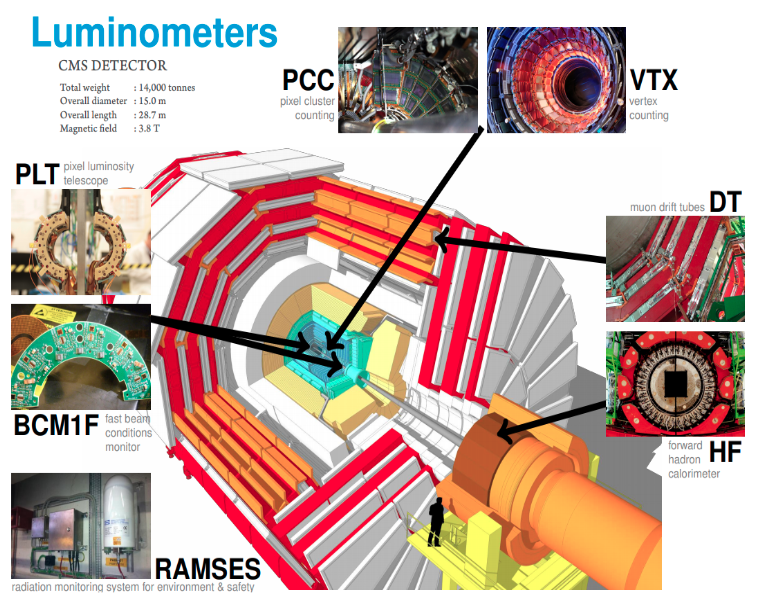
\includegraphics[width=0.9\textwidth]{ashish_thesis/luminometer_cms.png}
\caption[CMS luminometers]{%
   Compact muon solenoid (CMS) detector with all of the luminosity measurement devices showing PLT, BCM1F, HF, DT, PCC and RAMSES. 
}
\label{fig:lumino_cms}
\end{figure}


\begin{figure}[!htp]
\centering
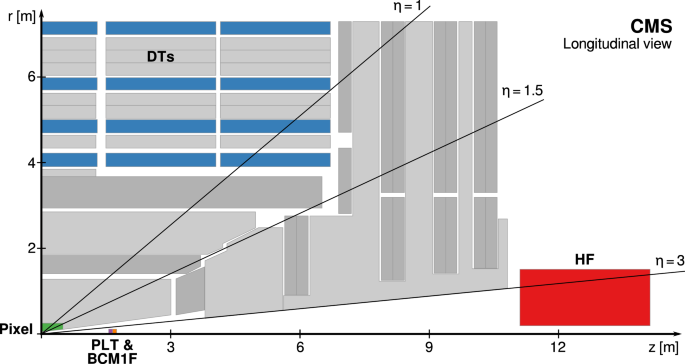
\includegraphics[width=0.9\textwidth]{ashish_thesis/luminometer_cms_pseudo.png}
\caption[Location of CMS luminometers]{%
    Cross section of the CMS detector in the r-z plane showing all Run 2 luminometer PLT, BCM1F, DTs, and HF location. The two RAMSES monitors used as a luminometer in Run 2 are located directly behind HF. 
}
\label{fig:lumino_cms_pseudo}
\end{figure}

%\newpage
\section{Pixel detector}

The pixel detector is one of the subdetectors of the CMS experiment that is closest to the interaction point where the proton beams collide. It consists of four barrel layers (L1-L4) at radii of 29, 68, 109 and 160 mm and three forward disks (D1-D3) on each end at distances of 291, 396, and 516 mm of pixel sensors from the center of the detector as shown in Fig.~\ref{fig:phaseI_upgrade}. It is built from 1856 silicon sensor modules, 1184 modules in the barrel layers (BPIX) and 672 modules for the forward disks (FPIX) \cite{Adam:2748381}. Modules for barrel layers and forward disks are shown in Fig.~\ref{fig:pixelmodule}. Table~\ref{tab:modpix} shows the number of modules in each pixel layer and disk. The modules in BPIX L1 are designed to handle high particle densities and radiation levels. Each module in this layer consists of a matrix of 4160 pixels, arranged in 160 rows and 26 columns. The pixel size in BPIX L1 is approximately 100x150 µm², which allows for high-resolution position measurements of charged particles. The modules in BPIX L2-4 layers are designed to withstand lower radiation levels compared to BPIX L1. Each module in BPIX L2-4 consists of a matrix of 66560 pixels, arranged in 260 rows and 256 columns. The pixel size in BPIX L2-4 is also approximately 100x150 µm². The FPIX modules are also designed to handle high particle densities and radiation levels. Each module in the FPIX consists of a matrix of 16128 pixels, arranged in 160 rows and 101 columns. The pixel size in the FPIX is approximately 100x150 µm². It provide high-precision position measurements of the charged particles produced in the collisions. These position measurements are used to reconstruct the trajectories of the particles and to identify the particles themselves. The pixel detector has a high position resolution, with a spatial resolution of 10-20 microns in the transverse direction and 20-30 microns in the longitudinal direction. The pixel detector also has a high time resolution, with a readout time of 25 nanoseconds. The pixel detector is capable of detecting charged particles with a wide range of energies, from a few hundred MeV to several TeV. The pixel detector is able to operate at very high particle fluxes, with a hit rate of up to $100 MHz/cm^2$. To achieve this high rate capability, the pixel detector uses fast readout electronics, which can read out the signals from the pixels in a few microseconds. The pixel detector is also designed to operate at a high radiation level, with a dose of up to $5 \times 10^{14} neutrons/cm^2$ expected over the lifetime of the detector. To mitigate the effects of radiation damage, the pixel detector uses sensors made of high-purity silicon and a cooling system that keeps the detector at a temperature of -20°C. The pixel detector is also used for the measurement of the luminosity at the CMS experiment. The luminosity measurement is based on counting the number of pixel clusters produced in the detector by the proton-proton collisions. The higher the collision rate, the more clusters are produced in the pixel detector. However, there are several challenges to accurately measure the luminosity with the pixel detector. One challenge is the high rate of particles that pass through the detector, which can cause pileup (multiple particles passing through the detector at the same time). Another challenge is the non-linearity of the pixel detector response, which can lead to inaccuracies in the luminosity measurement. Therefore, the motivation of this research work is to develop and test more precise techniques for measuring the luminosity with the pixel detector, in order to improve the precision of the luminosity measurement and to better understand the effects of detector response on the measurement.

\begin{figure}[!htp]
\centering
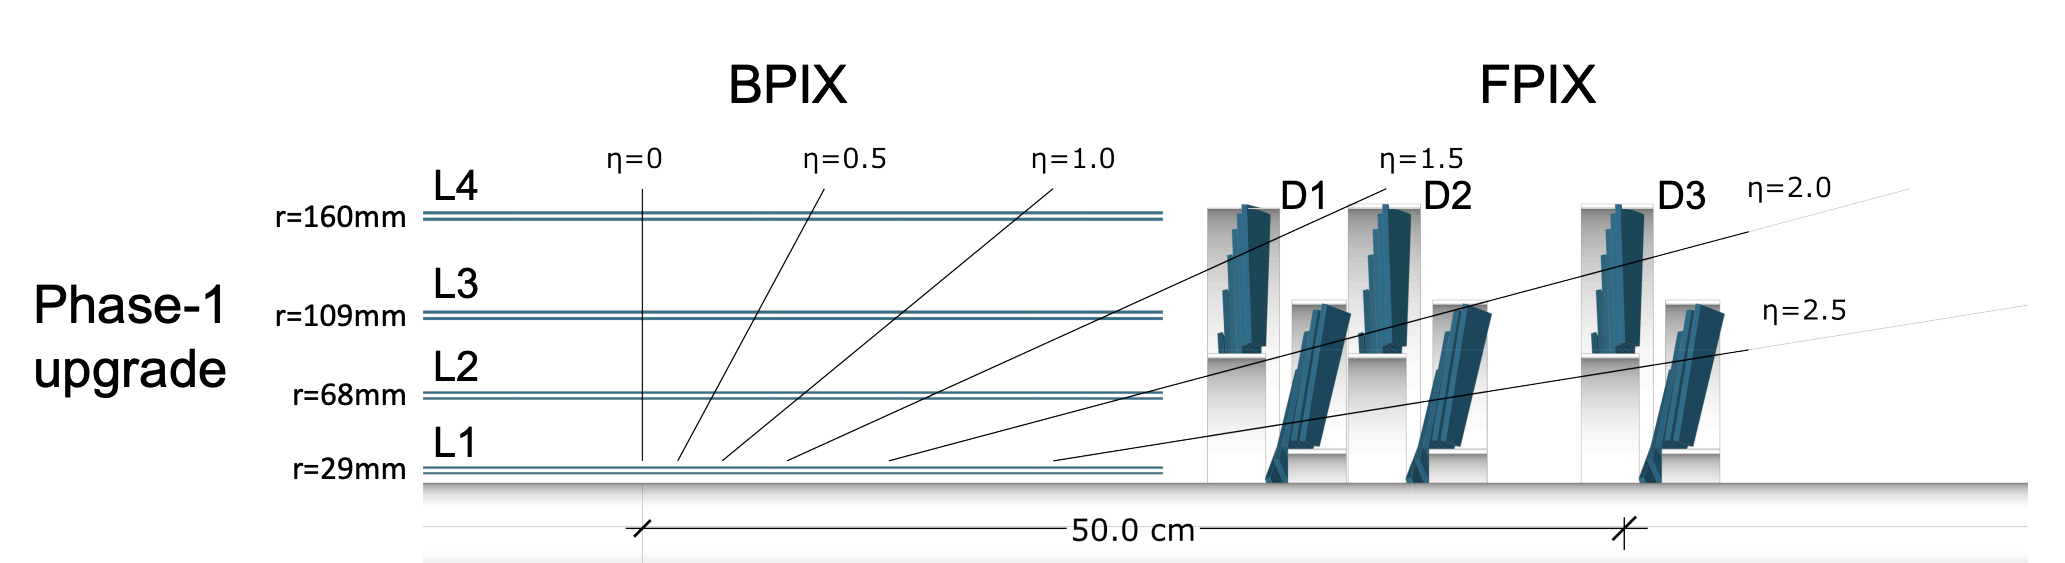
\includegraphics[width=1\textwidth]{ashish_thesis/phaseI_upgrade_pixel_detector.png}
\caption[Pixel detector layout]{%
   Layout of the CMS Phase-1 upgraded pixel detector in longitudinal view. 
}
\label{fig:phaseI_upgrade}
\end{figure}


\begin{figure}[!htp]
\centering
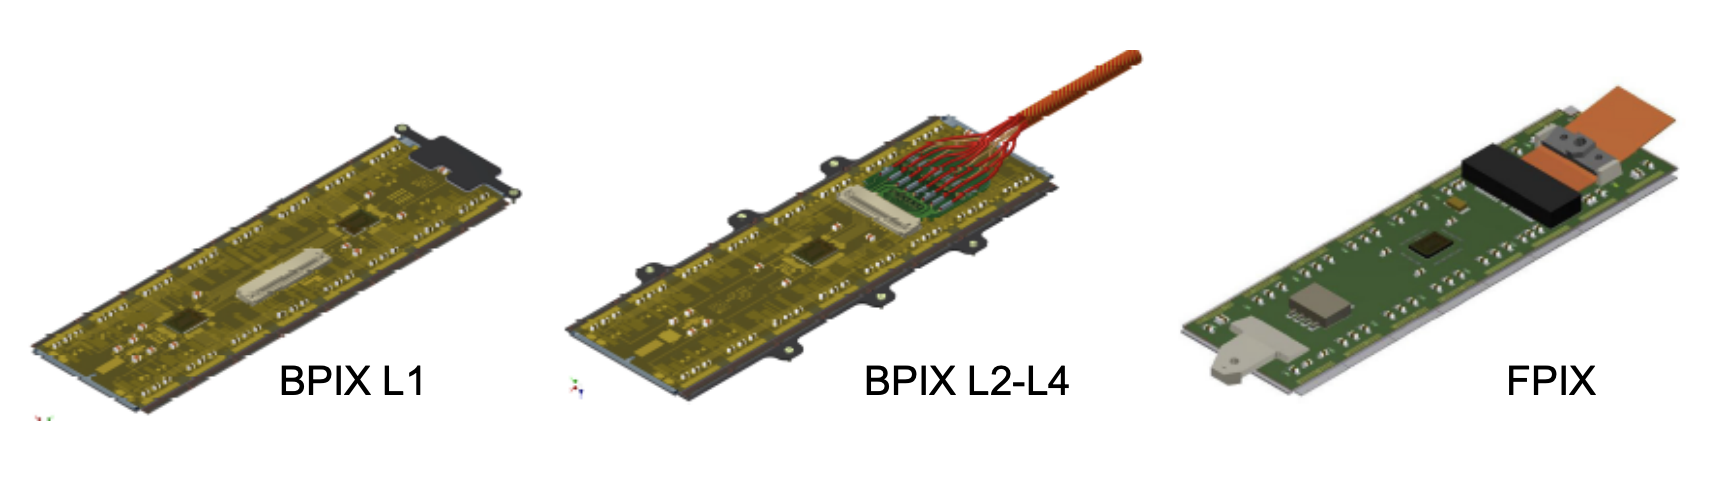
\includegraphics[width=1\textwidth]{ashish_thesis/silicon_pixel_module.png}
\caption[Design of pixel module]{%
   Pixel detector modules for BPIX L1 (left), BPIX L2-4 (middle), and
the FPIX detector (right). 
}
\label{fig:pixelmodule}
\end{figure}


\begin{table}
  \begin{center}
    \begin{tabular}{ccccc}  
    \textbf{Layer/Disk}   & \textbf{\# modules} \\ \hline
     L1      &    96        \\  
       L2    &     224   \\ 
        L3   &       352 \\ 
         L4   &       512 \\ 
         D1 inner ring & 88     \\ 
         D1 outer ring &   136    \\ 
         D2 inner ring &      88 \\ 
         D2 outer ring &   136   \\ 
          D3 inner ring&     88  \\ 
         D3 outer ring &    136  \\ 
      \end{tabular}
    \caption[\# modules in pixel layers and disks]{Number of pixel detector modules in each layer and disk.}
    \label{tab:modpix}
  \end{center}
\end{table}



\section{Pixel cluster counting (PCC) method}

The Pixel Cluster Counting (PCC) method is one of the main luminosity measurement methods used at the CMS experiment. The PCC method is based on counting the number of pixel clusters produced by the collisions in the CMS pixel detector, which is a high-resolution silicon detector located close to the collision point. The pixel detector is made up of more than 65 million pixels, each of which is 100 micrometers by 150 micrometers in size. The detector is designed to detect charged particles produced in the collisions, and the pixel clusters are formed when several neighboring pixels are hit by a single particle. The PCC method is based on the assumption that the number of pixel clusters produced is proportional to the number of collisions, and therefore to the luminosity. The proportionality constant is called the pixel detector visible cross section, and it can be determined from a calibration measurement. The PCC method is implemented in two stages: the online and offline stages. In the online stage, the pixel clusters are counted in real time by the CMS data acquisition system, which uses a custom-designed ASIC chip to process the pixel detector signals. The online luminosity measurement is therefore available within seconds of the collisions, and it is used to monitor the stability of the detector and to provide feedback to the LHC operators. In the offline stage, the raw data from the pixel detector is analyzed using dedicated software to determine the pixel clusters and to calculate the luminosity. The offline luminosity measurement is more accurate than the online measurement, as it takes into account various corrections and calibrations that are not possible in real time. The offline luminosity measurement is also used to determine the absolute luminosity scale, which is obtained from beam parameters. There are several steps involved in the PCC method for measuring luminosity as described below.

\begin{itemize}

\item Pixel detector data acquisition is the process of collecting and digitizing the signals from the silicon pixel detectors in the CMS experiment. When a particle passes through the silicon pixel detector, it creates a small amount of charge in the pixel sensor. The charge is collected by the electrodes in the pixel sensor and converted into a voltage signal. The voltage signal is then digitized using an analog-to-digital converter (ADC) to create a digital signal. The ADC measures the voltage at regular intervals, called sampling intervals, and assigns a digital value to each voltage measurement. The digital signal is then stored in a buffer in the front-end electronics of the pixel detector. The buffer is a small amount of memory that temporarily holds the data before it is transmitted to the data acquisition system. The data acquisition system continuously monitors the data from the pixel detectors to detect interesting events. When an event of interest is detected, a trigger signal is sent to the front-end electronics of the pixel detector to read out the data from the buffer. The readout electronics in the pixel detector then transmit the data to the data acquisition system using high-speed optical fibers. The data is sent in packets, called data frames, which contain information about the event, such as the time of the event, the position of the particle, and the amount of charge deposited in the pixel sensor. The data acquisition system processes the data frames to reconstruct the particle tracks and identify the types of particles that passed through the pixel detector. The data is then stored in a format that can be used for further analysis.

\item Pixel cluster reconstruction is the process of identifying groups of adjacent pixels that have been fired by a single particle passing through the detector. The first step in the pixel cluster reconstruction process is to identify individual pixel hits in the data frames obtained from the pixel detector data acquisition system. A pixel hit is a small region of the pixel detector where charge has been deposited by a particle. The next step is to identify "seed" pixels, which are individual pixels with a high signal-to-noise ratio. A seed pixel is defined as a pixel hit with a signal above a certain threshold, which is typically set at a few times the noise level of the pixel detector. Once seed pixels have been identified, the next step is to build pixel clusters around each seed pixel. This is done by adding adjacent pixels with a signal above a lower threshold, called the cluster threshold. The cluster threshold is typically set at a level that minimizes the number of fake clusters while maximizing the efficiency of cluster finding. After pixel clusters have been built, the next step is to split or merge clusters as needed. This is done to remove fake clusters caused by noise or overlapping particles, and to merge clusters that are split due to inefficiencies in the cluster building process. Once the pixel clusters have been identified and merged/split as necessary, they are parameterized by their position and energy. The position of the cluster is determined by the center of gravity of the pixels in the cluster, and the energy is determined by summing the signal of all the pixels in the cluster. Finally, a set of selection criteria are applied to the pixel clusters to remove any remaining fake clusters and select only those clusters that are likely to be from real particle interactions. These selection criteria typically include requirements on the size, shape, and energy of the clusters.

\item The number of pixel clusters is counted for a given time interval, known as lumi section. One lumi section is 23.36 seconds time interval. The first step in the pixel cluster counting process is to select events of interest from the large dataset obtained from the CMS experiment. This is typically done using trigger systems that select events that are likely to be of interest based on their energy, particle multiplicity, or other criteria. Once the events of interest have been selected, the next step is to reconstruct the pixel clusters in each event using the algorithm described in the previous bullet point. This involves identifying individual pixel hits, identifying seed pixels, building pixel clusters around each seed pixel, and parameterizing the clusters. After the pixel clusters have been reconstructed in each event, the next step is to count the number of clusters in each event. This can be done using simple counting algorithms that count the number of clusters above a certain energy threshold, or more sophisticated algorithms that use machine learning techniques to identify and count clusters. The number of pixel clusters in each event is affected by various sources of background noise, such as electronic noise and cosmic ray background. To accurately measure the number of signal clusters in each event, these background sources must be subtracted from the total cluster count. This can be done using techniques such as sideband subtraction or template fitting. Finally, to obtain an accurate measurement of the number of particles that passed through the pixel detector, the cluster counts must be corrected for the inefficiencies in the cluster reconstruction process. This can be done using simulation or other techniques to estimate the efficiency of the cluster finding algorithm as a function of the particle energy, position, and type.

\item The number of pixel clusters is calibrated to account for various factors that affect the luminosity measurement, such as the efficiency of the pixel detector and the beam intensity. The calibration step is an important part of the PCC (Pixel Cluster Counting) method for measuring luminosity at the CMS experiment. The purpose of calibration is to account for various factors that can affect the measurement of the number of pixel clusters, which is directly proportional to the number of collisions that occurred during a given time interval. These factors include the efficiency of the pixel detector and the beam intensity. The efficiency of the pixel detector refers to the probability that a charged particle passing through the detector will create a signal in one or more pixels. The efficiency of the detector can vary with time, and it can also depend on the energy and angle of the charged particle. To account for the detector efficiency, calibration factors are applied to the number of pixel clusters that are counted. These calibration factors are determined by comparing the number of pixel clusters measured by the detector to the number of collisions predicted by other detectors or simulations. The beam intensity refers to the number of protons circulating in the LHC at any given time. The beam intensity can vary over time and can affect the measurement of the collision rate. To account for the beam intensity, the number of pixel clusters is normalized by the instantaneous luminosity, which is a measure of the collision rate at the interaction point. The instantaneous luminosity is determined by other detectors or by theoretical calculations. After applying the calibration factors, the number of pixel clusters is converted to the number of collisions that occurred during the given time interval. This number is then used along with other parameters such as the frequency at which the LHC is operating and the size of the interaction region to calculate the luminosity of the collision using the formula $L = \frac{N_{cl}  f_{rev}} {\sigma_{vis}} $. The resulting luminosity measurement provides valuable information about the collision rate and the physics processes occurring at the CMS experiment.

\item The number of pixel clusters is used to calculate the luminosity using the following formula:

\begin{equation}
 L = \frac{N_{cl} f_{rev} } {\sigma_{vis}}   
\end{equation}

where L is the luminosity, $N_{cl}$ is the number of clusters, $f_{rev}$ is the revolution frequency of the LHC, and $\sigma_{vis}$ is the visible cross section of the interaction region.

\end{itemize}


\section{Advantages of the pixel cluster counting method}

The PCC method has several advantages over the other luminosity measurement methods used by the CMS experiment. One advantage is its high precision and stability, as it is based on a well-understood physical process and has a small systematic uncertainty. %Another advantage is its independence from the beam conditions, as the pixel detector is insensitive to the beam halo and the beam-gas interactions.
The PCC method is also robust against pile-up, which is the presence of multiple proton-proton interactions in a single bunch crossing, as it can distinguish between pixel clusters produced by different collisions. The PCC method is based on the pixel detector, which has a high spatial resolution and can accurately measure the position and energy of charged particles. This allows for precise measurements of the luminosity, even when the particle collision rate is high. Advantages of the PCC method are described below,

\begin{itemize}

\item High precision: The pixel detector has a high granularity and can detect individual particles with high precision. This allows for a precise measurement of the luminosity, with uncertainties typically below 2\%.

\item High efficiency: The pixel detector has a high detection efficiency, meaning that it can detect a large fraction of the particles produced in the collisions. This allows for a high signal-to-noise ratio and a low level of background noise, resulting in a more accurate measurement of the luminosity.

\item Long-term stability: The pixel detector has a high level of stability over long periods of time, which is important for accurate luminosity measurements over extended periods of data-taking.

%\item Fast and real-time: The pixel cluster counting method can provide luminosity measurements in real-time, allowing researchers to quickly analyze the data and make adjustments to the experiment as needed. This is particularly important for experiments that need to optimize their data-taking strategies based on the luminosity measurements.

\item Low sensitivity to pileup: Pileup refers to the number of additional collisions that occur within the same bunch crossing as the primary collision being studied. The pixel cluster counting method is relatively insensitive to pileup, meaning that it can still provide accurate luminosity measurements even when pileup is high.

\item Wide dynamic range: The pixel cluster counting method has a wide dynamic range, meaning that it can measure luminosities over a wide range of values, from low to high. This is important for experiments that need to measure luminosities over different energy ranges.

\item Insensitivity to beam conditions: The pixel cluster counting method is relatively insensitive to beam conditions such as beam intensity and beam size. This makes it a reliable technique for luminosity measurement, even when the beam conditions vary.

\item Independent of beam crossing angle: The pixel cluster counting method is independent of the beam crossing angle, which is the angle at which the beams intersect. This makes it easier to compare results obtained under different beam crossing angles.


\item Independence from trigger systems: The PCC method operates independently of the CMS experiment's trigger systems, which means it is not affected by any biases or inefficiencies that might be present in the trigger.

\end{itemize}

%However, the PCC method also has some limitations and challenges. One limitation is its sensitivity to the pixel detector efficiency and the noise level, as the cluster formation probability depends on the number of hit pixels and their signal-to-noise ratio. The PCC method also requires a precise knowledge of the pixel cluster cross section, which can be affected by various factors such as the beam spot size, the beam divergence, and the pile-up conditions. The PCC method is also affected by various sources of background, such as cosmic rays, machine-induced noise, and photon conversions, which can mimic pixel clusters produced by collisions. To mitigate these limitations and challenges, the CMS employs several techniques and strategies in the PCC method. One technique is the use of pixel clustering algorithms that are optimized for different beam conditions and pile-up levels, and that incorporate various quality criteria to reject noisy and fake clusters. Another technique is the use of dedicated calibration measurements using known luminosity sources, such as Van der Meer scans and beam-gas events, which provide a precise determination of the pixel cluster cross section and its variations as a function of the beam conditions. The CMS also employs various data-driven and simulation-based methods to estimate the background contributions and their uncertainties, and to correct for their effects on the luminosity measurement.

The PCC method has been extensively tested and validated by the CMS during the LHC Run 1 and Run 2, which corresponded to proton-proton collisions at center-of-mass energies of 7-8 TeV and 13 TeV, respectively. The PCC method has achieved a relative luminosity precision of about 2-3 \%, which is well within the design goals of the CMS \cite{CMS-PAS-LUM-18-002}. In the future, the PCC method will continue to be a key component of the CMS luminosity measurement strategy, as it provides a precise and robust measurement of the luminosity ratio between different datasets and periods. The PCC method will also benefit from the upgrades and improvements planned for the CMS pixel detector and the LHC, which will increase the luminosity and the collision rate, and will challenge the performance and the calibration of the PCC method. The CMS is planning to install a new pixel detector for the High-Luminosity LHC (HL-LHC) era, which will feature smaller pixel sizes, faster readout electronics, and radiation-hard materials. The CMS is also planning to develop new techniques and algorithms for the PCC method, such as machine learning methods, deep neural networks, and real-time analysis tools.

%The Pixel Cluster Counting (PCC) method is a powerful and reliable technique for measuring the luminosity of proton-proton collisions at the CMS detector at the LHC. The PCC method is based on the counting of pixel clusters produced by the collisions in the CMS pixel detector, and it provides a precise and stable measurement of the relative luminosity between different datasets and periods. The PCC method has several advantages, such as its high precision, stability, and independence from the beam conditions, and it has several limitations and challenges, such as its sensitivity to the pixel detector efficiency and the noise level, and its dependence on the pixel cluster cross-section and the background contributions. The PCC method has been extensively tested and validated by the CMS, and it will continue to play a crucial role in the future physics program of the CMS and the LHC.

%Pixel Cluster Counting (PCC) is a method for measuring the luminosity of particle collisions in high-energy physics experiments, such as those conducted at the Large Hadron Collider (LHC). The PCC method is based on counting the number of clusters of charged particles produced in the collision that are detected by the pixel detector of the experiment.

%Measuring the luminosity of particle collisions is an essential part of high-energy physics experiments. Luminosity is a measure of the rate at which particles are colliding and is directly related to the number of events observed in the experiment. The luminosity measurement is critical for understanding rare physics processes, such as the production of new particles or the measurement of the properties of known particles.

%Several techniques are used to measure luminosity in particle physics experiments, including the use of scintillators, Cherenkov detectors, and other radiation detectors. However, the most commonly used technique is the measurement of the rate of particles produced in the collision.

%The PCC method is based on counting the number of clusters of charged particles produced in the collision that are detected by the pixel detector of the experiment. The pixel detector is a high-resolution detector that is designed to provide precise measurements of the position and energy of charged particles.

%In the PCC method, the charged particles produced in the collision pass through the pixel detector, where they create clusters of pixels that are read out by the detector electronics. The number of clusters produced in each collision is proportional to the luminosity of the collision.

%In conclusion, the PCC method is a powerful technique for measuring the luminosity of particle collisions in high-energy physics experiments. The PCC method is based on counting the number of clusters of charged particles produced in the collision that are detected by the pixel detector of the experiment. The PCC method has several advantages over other luminosity measurement techniques, including its high spatial resolution, insensitivity to background radiation, insensitivity to the energy of the charged particles, and insensitivity to the material used in the detector. These advantages make the PCC method a valuable tool for understanding rare physics processes in particle physics experiments.

%Pixel cluster counting is the process of counting the number of pixel clusters that are reconstructed from the data acquired by the silicon pixel detectors during a given time interval, known as an LHC orbit. An orbit is the time it takes for the LHC to complete one revolution.

%The pixel detectors record the energy deposited by particles passing through them, and the data from the detectors is acquired by the CMS data acquisition system. The acquired data is then processed to reconstruct pixel clusters. A pixel cluster is a group of adjacent pixels that have been fired by a single particle passing through the detector. Pixel clusters are reconstructed using algorithms that take into account the shape and size of the charge deposited by the particles in the pixels.

%Once the pixel clusters are reconstructed, they are counted for a given time interval, typically the duration of one LHC orbit, which is about 89 microseconds. The number of pixel clusters is directly proportional to the number of collisions that occurred during that time interval. Therefore, counting the number of pixel clusters provides a way to measure the collision rate, which is an important input for calculating the luminosity of the collision.

%However, it is important to note that not all pixel clusters correspond to actual collisions. Some pixel clusters may be produced by background events, such as cosmic rays, that are not relevant for measuring the collision rate. Therefore, it is necessary to calibrate the number of pixel clusters to account for various factors that affect the luminosity measurement, such as the efficiency of the pixel detector and the beam intensity, before using it to calculate the luminosity.


\newpage
\section{Previous studies on PCC luminosity measurement}


The Pixel Cluster Count (PCC) of various layers and disks, normalized to the total PCC, as a function of luminosity section can provide crucial insights into the detector's performance and stability over time and under different conditions \cite{CMS-PAS-LUM-15-001}\cite{CMS-PAS-LUM-16-001}. A luminosity section is a unit of data-taking time in the LHC, typically lasting about 23.36 seconds, during which the beam conditions are assumed to be stable. The luminosity delivered during each of these sections can vary, leading to different levels of activity in the detector.

When these ratios are plotted against lumi sections, several key aspects can be studied:

\begin{itemize}
\item Detector Stability: Stable ratios across lumi sections suggest that the detector is functioning consistently and reliably under varying luminosity conditions. Abrupt spikes or drops could be indicative of potential problems such as radiation damage, electronic noise, or other instabilities in the detector.

\item Long-Term Performance: By tracking these ratios over multiple lumi sections, one can monitor the long-term performance of the detector. This approach allows for the detection of gradual changes or trends, which could suggest a slow degradation of the detector components.

\item Layer/Disk-Specific Analysis: This type of plot can reveal layer or disk-specific issues. For instance, if one layer's PCC ratio deviates significantly from the norm in high luminosity sections, it might suggest that this layer is particularly sensitive to high luminosity or is underperforming.

\item Operational Adjustments: Observations from these plots can guide operational adjustments. If the PCC ratios for certain layers or disks consistently deviate under specific luminosity conditions, adjustments could be made in the detector operation to account for these variations.
\end{itemize}


The stability plots of the pixel detector for Run2018A, Run2018B and Run2018C are shown in Fig.~\ref{fig:RunA_PCC_ratios}, Fig.~\ref{fig:RunB_PCC_ratios}, Fig.~\ref{fig:RunC_PCC_ratios} respectively where the PCC ratios are not stable for some layers and disks with time. These PCC ratios as a function of luminosity sections, where each section represents about 23.36 seconds of data collection, allows physicists to conduct a nuanced evaluation of the pixel detector's performance and stability, identify potential issues, and make necessary operational modifications to ensure the detector's efficiency. 


\begin{figure}[!htp]
\centering
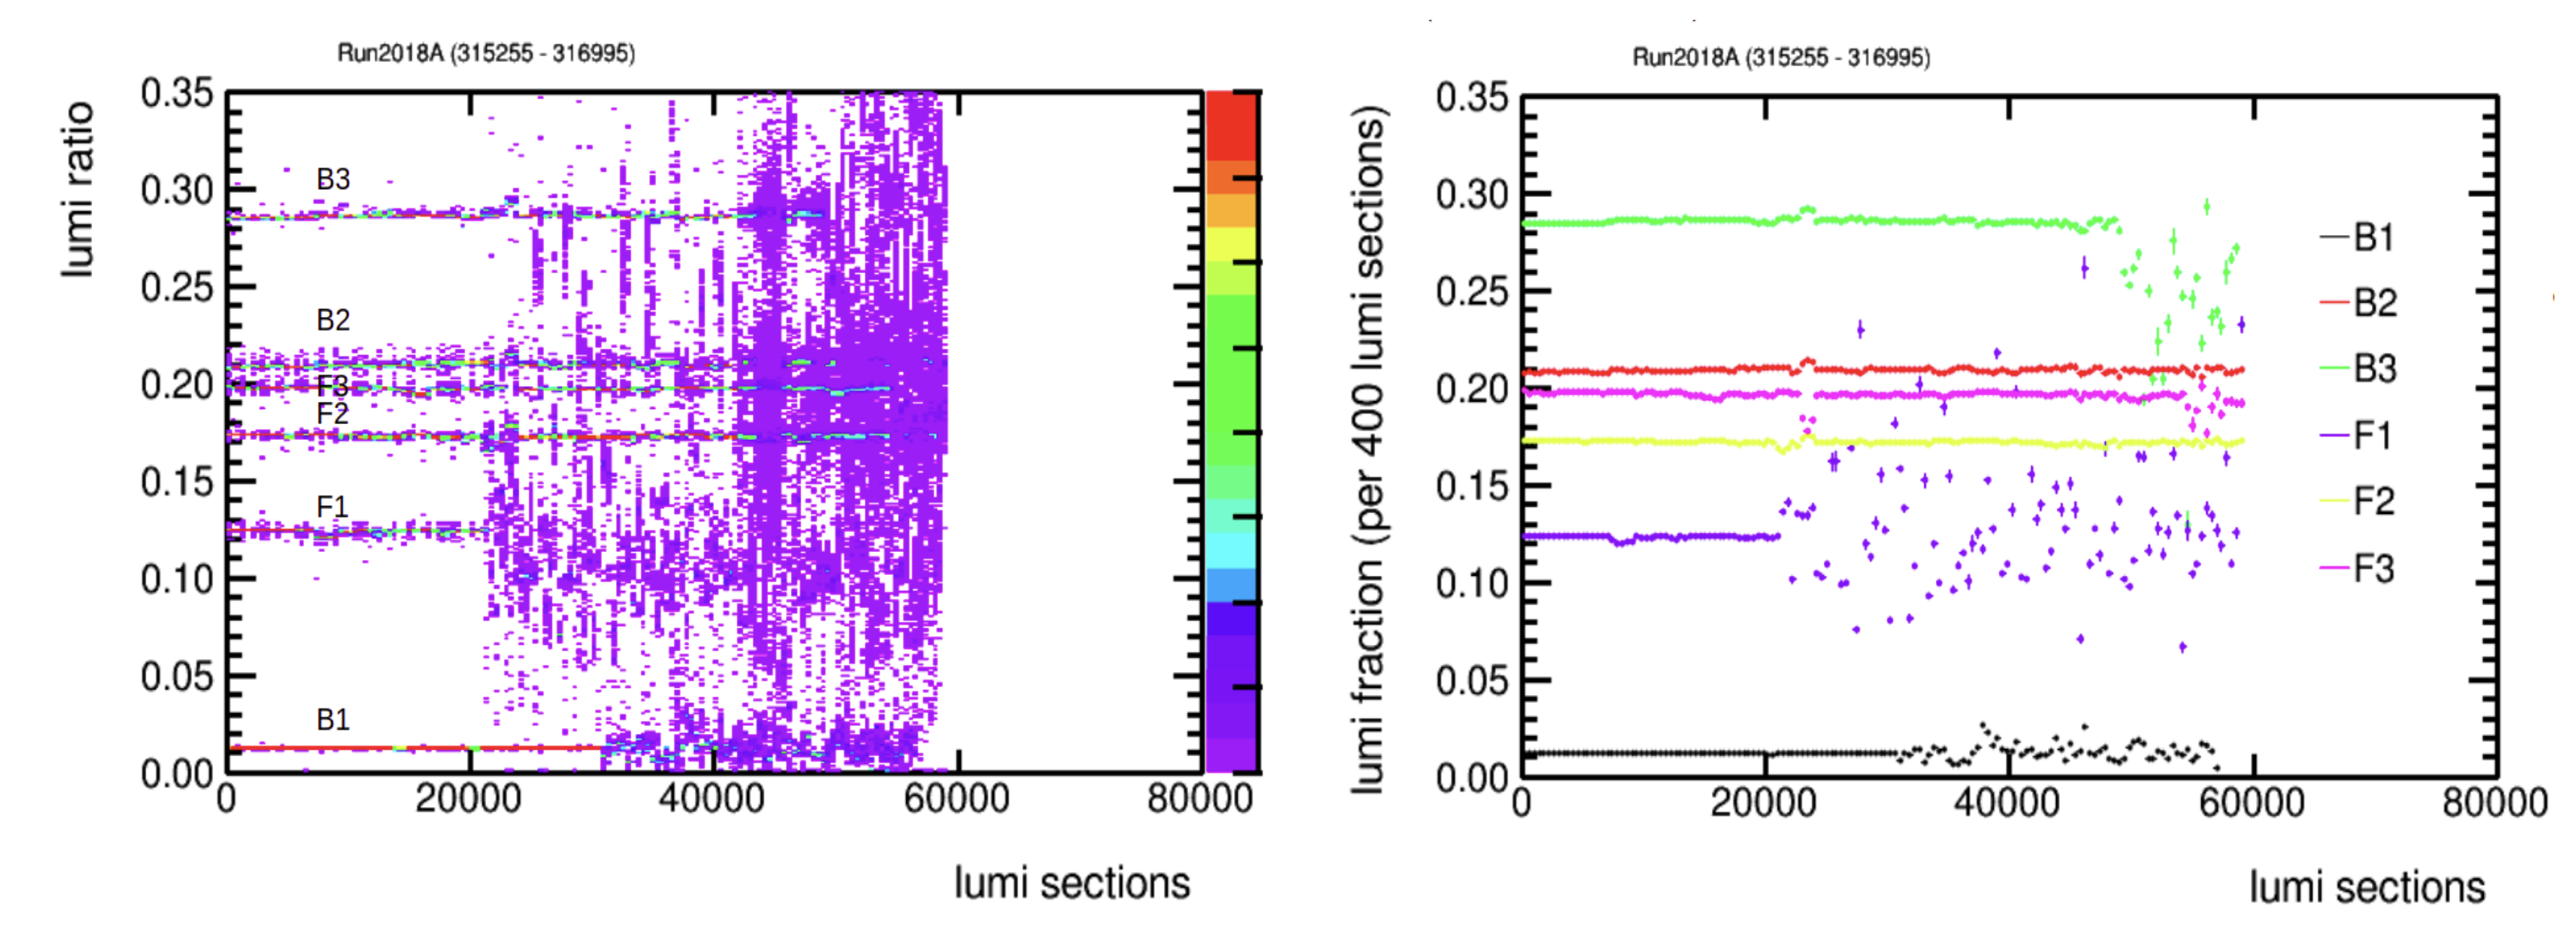
\includegraphics[width=1\textwidth]{ashish_thesis/Run2018A_old.png}
\caption[PCC ratios for period 2018A]{%
Left: Luminosity ratios for various sub detectors L2, L3, L4, D1, D2, D3 of pixel detector as a function of lumi section for Run2018A. Right: X Profile of luminosity ratios vs lumi section graph for various sub detectors L2, L3, L4, D1, D2, D3 of pixel detector showing luminosity fraction as a function of lumi section for Run2018A.

}
\label{fig:RunA_PCC_ratios}
\end{figure}


\begin{figure}[!htp]
\centering
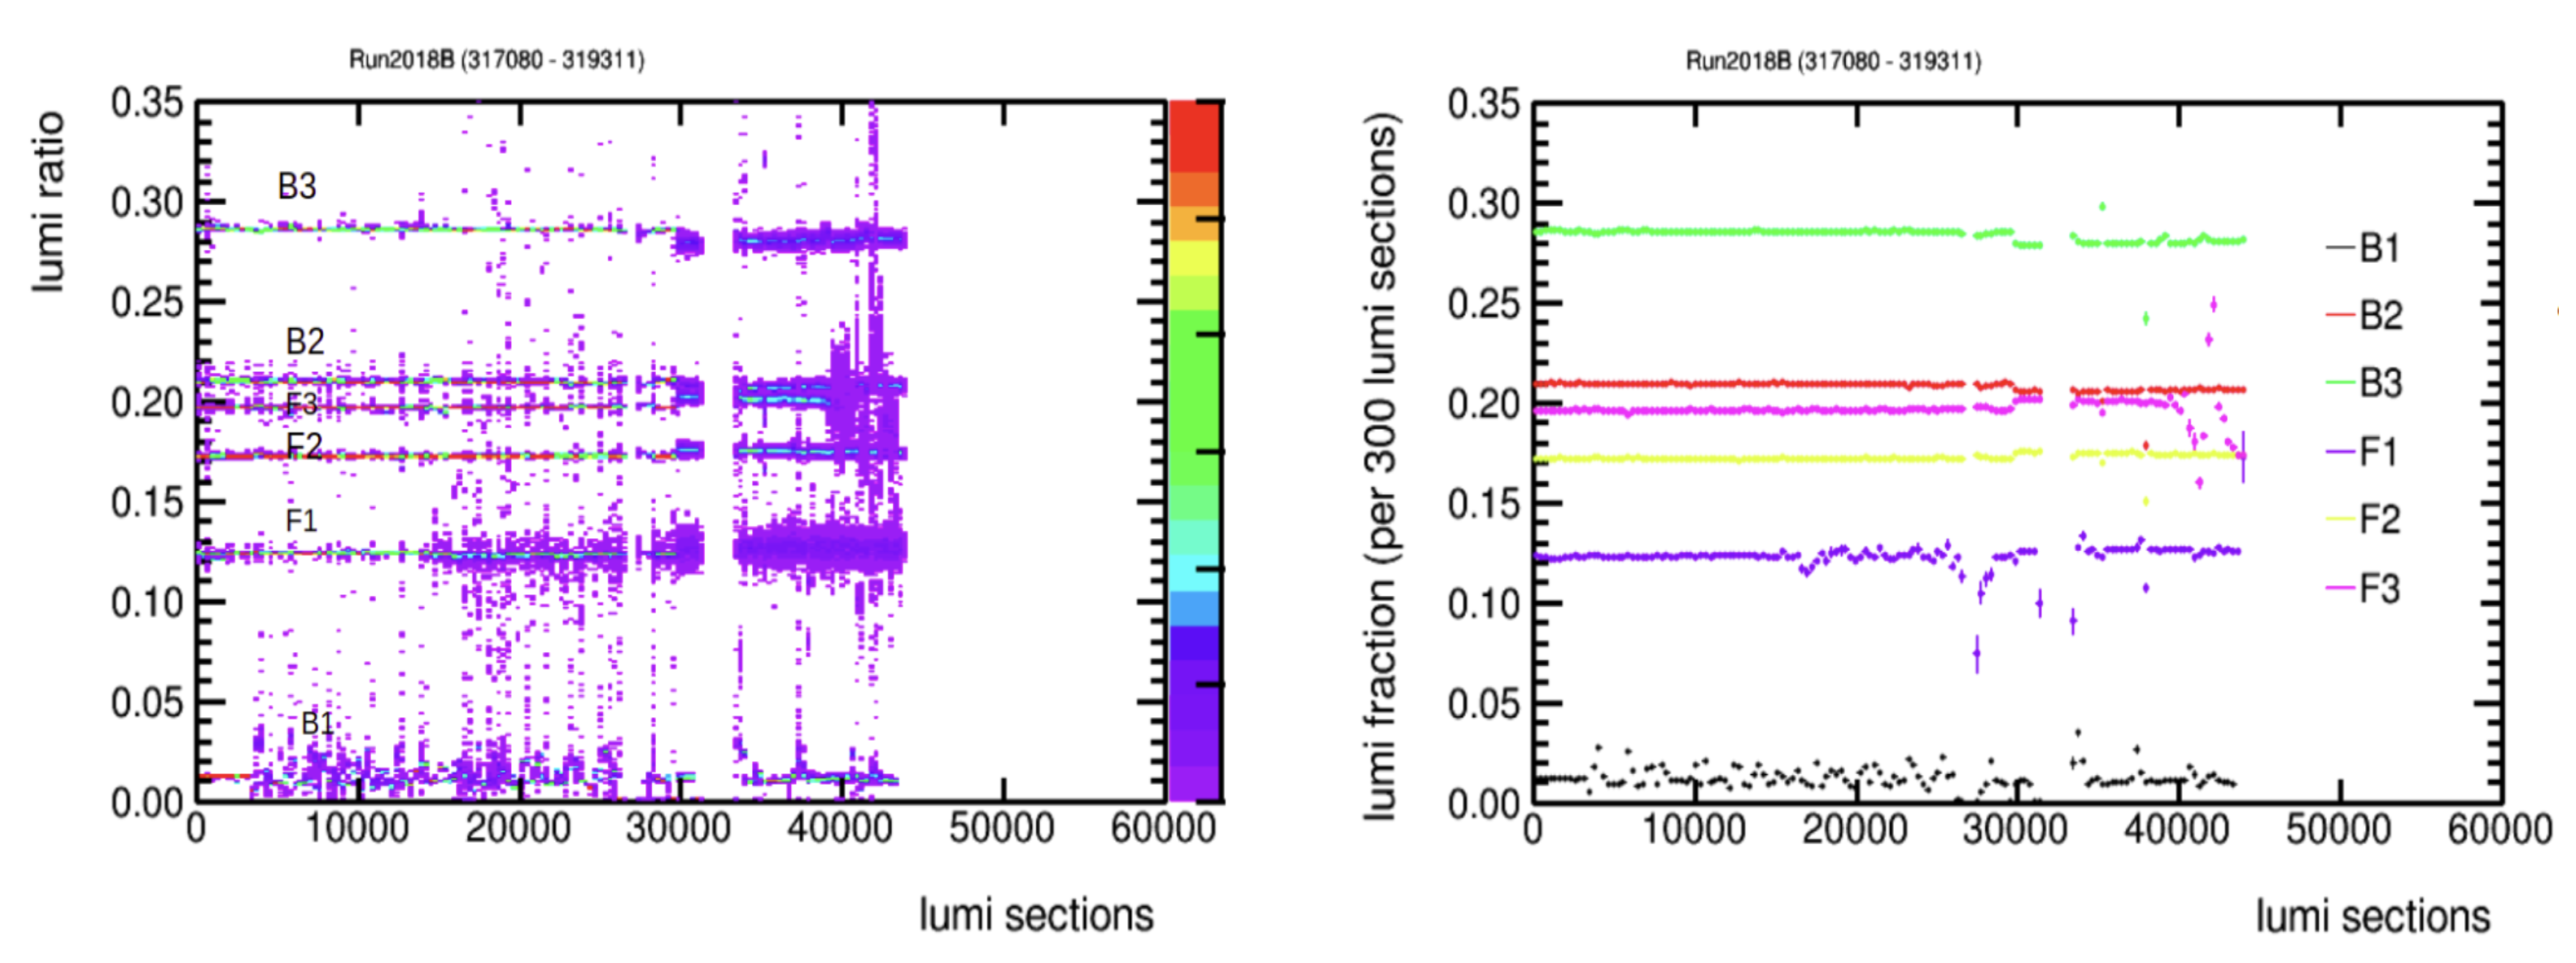
\includegraphics[width=1\textwidth]{ashish_thesis/Run2018B_old.png}
\caption[PCC ratios for period 2018B]{%
Left: Luminosity ratios for various sub detectors L2, L3, L4, D1, D2, D3 of pixel detector as a function of lumi section for Run2018B. Right: X Profile of luminosity ratios vs lumi section graph for various sub detectors L2, L3, L4, D1, D2, D3 of pixel detector showing luminosity fraction as a function of lumi section for Run2018B.
}
\label{fig:RunB_PCC_ratios}
\end{figure}


\begin{figure}[!htp]
\centering
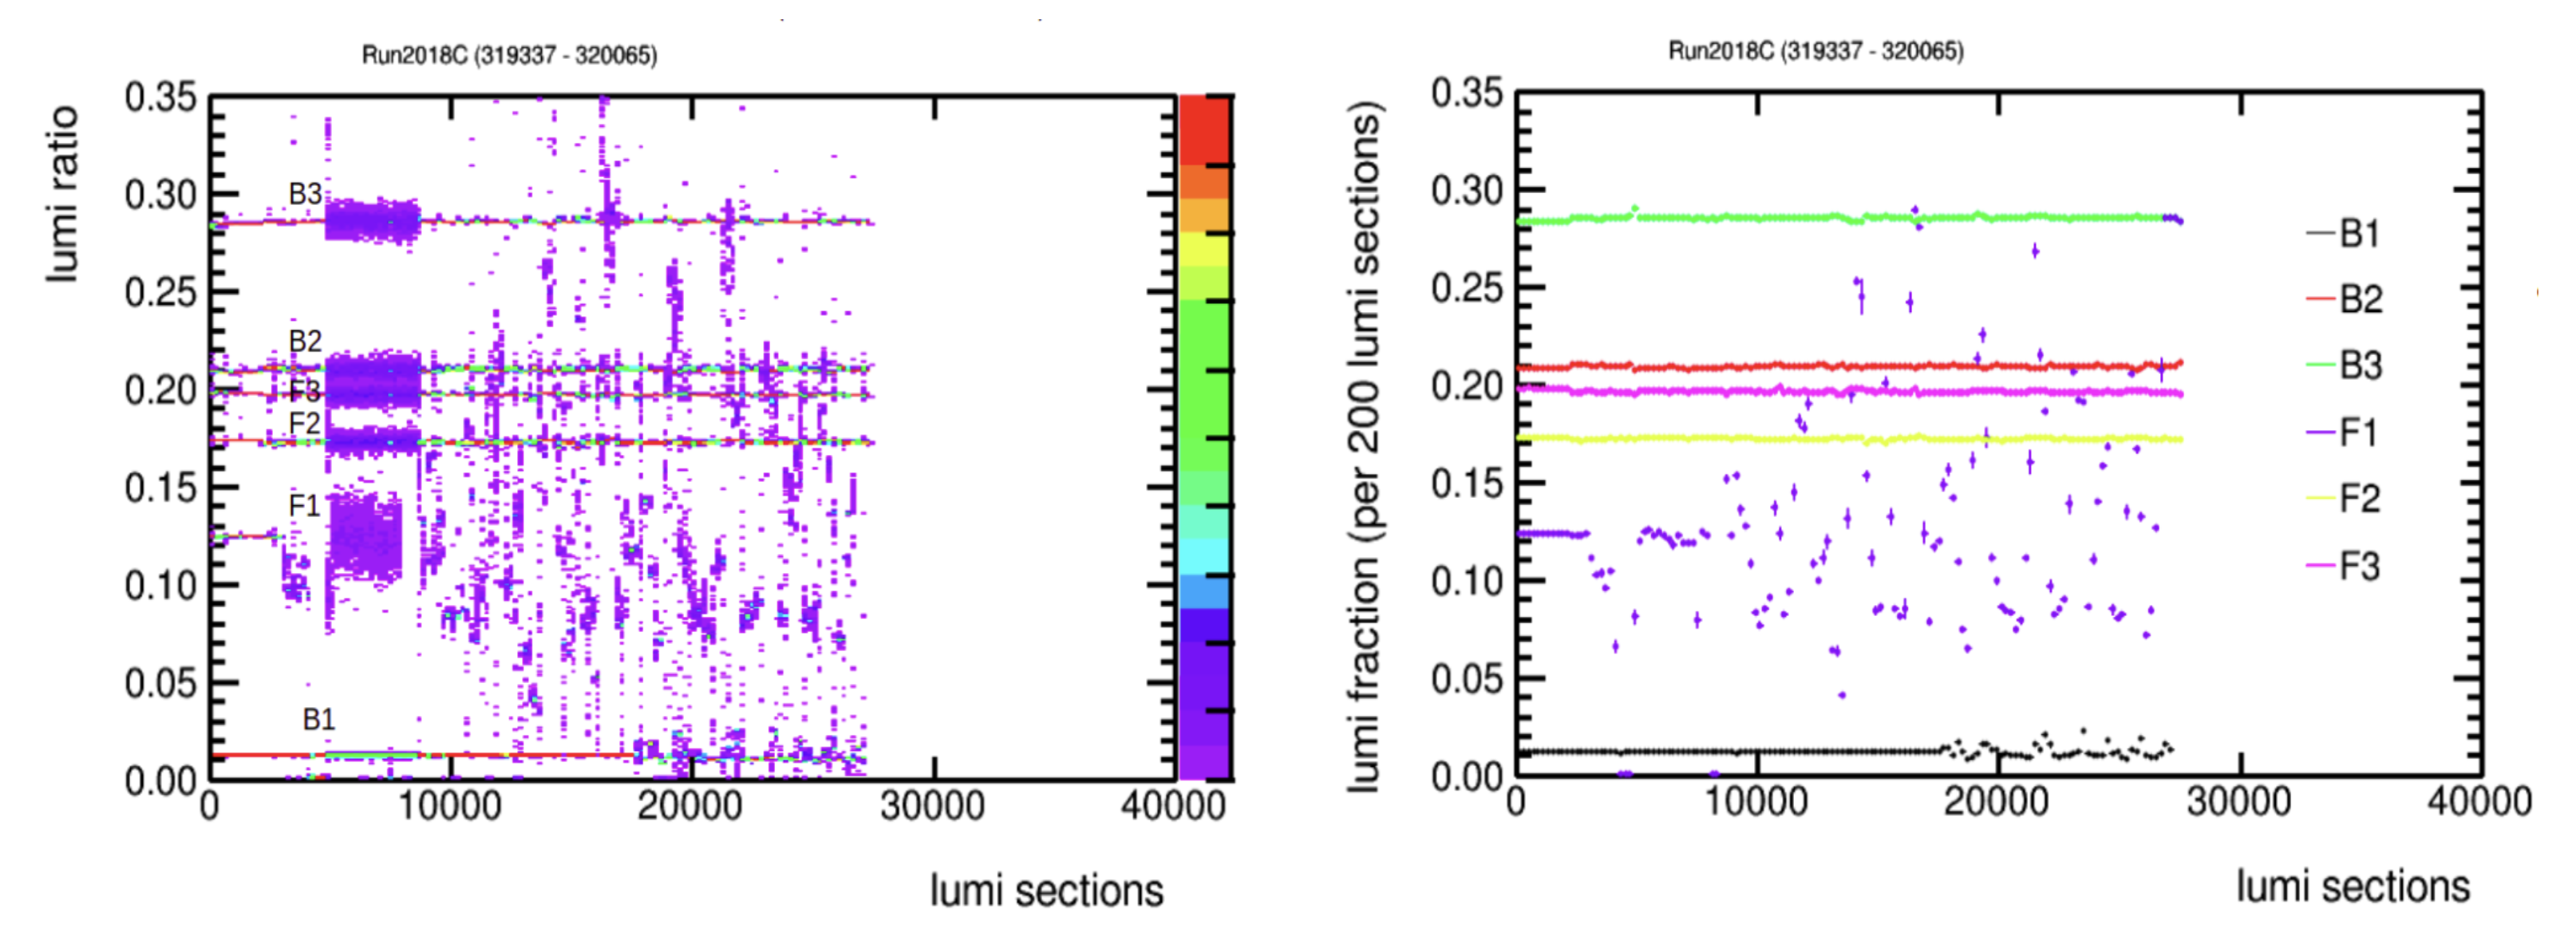
\includegraphics[width=1\textwidth]{ashish_thesis/Run2018C_old.png}
\caption[PCC ratios for period 2018C]{%
Left: Luminosity ratios for various sub detectors L2, L3, L4, D1, D2, D3 of pixel detector as a function of lumi section for Run2018C. Right: X Profile of luminosity ratios vs lumi section graph for various sub detectors L2, L3, L4, D1, D2, D3 of pixel detector showing luminosity fraction as a function of lumi section for Run2018C.
}
\label{fig:RunC_PCC_ratios}
\end{figure}

	\chapter{Luminometer Calibration}
\label{ch3}

\section{Van Der Meer Method}

The Van Der Meer (vdM) scan let us obtain the value of $\sigma_{visible}$ using different luminometers. For this case the detector of interest is the pixel detector with which are going to obtain a calibration of the luminosity using the vdM scan in combination with the PCC method. The scan consist on separating particle the beams from each other between the X and Y axis by $\Delta X$ and $\Delta Y$ values moving them and recording values of luminosity independently, when the scan on X and scan on Y are imposed over each other we said that they're on head on giving the maximum value of luminosity. Usually a single gaussian fit is used to obtain beam overlap widths also denoted as $\Sigma_{x}$ and $\Sigma_{y}$, other fit models may be used like the doble gaussian depending on the quality of the fit \cite{Vdm}

\begin{figure}[h]
    \centering
    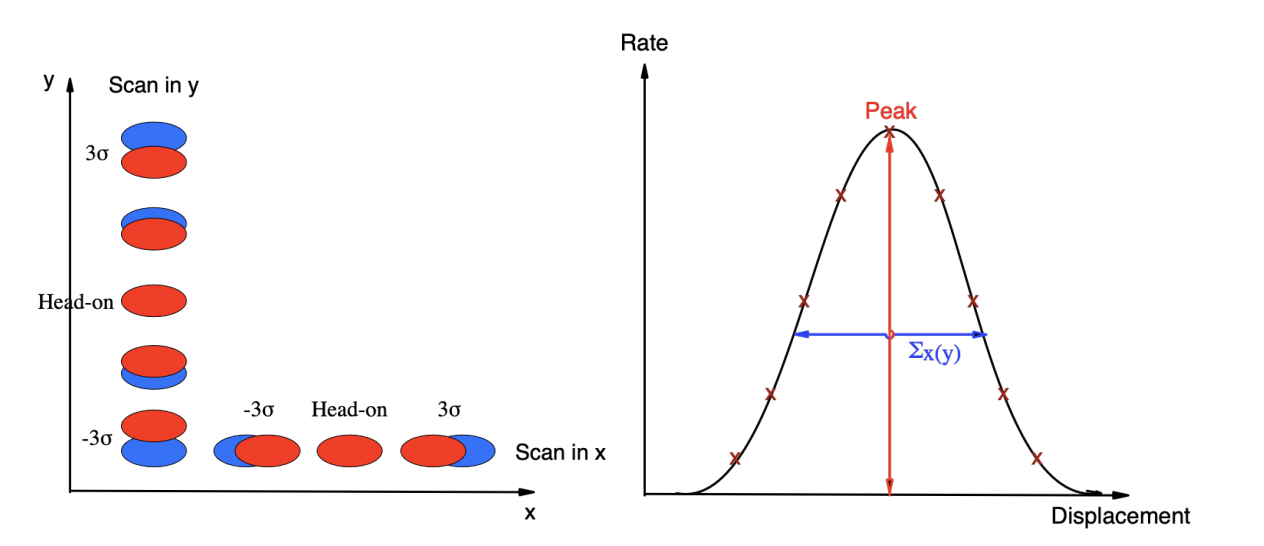
\includegraphics[width=1\textwidth]{vdm1.png}
    \caption{The vdm scan on the left showing the beams for X and Y. On the right a curve of the different values of rate for the beams displacement, the peak occurs during the head on part.}
    \label{fig:vdm1}
\end{figure}


For obtaining the importnat parameters on the vdm scan we return to the equation (1.2) and apply it to and individual bunch crossing, the values of N1 and N2 being the number of protons colliding can be obtained since is a known quantity from the experiment, the frequency f is also a known quantity, the frequency of the LHC which is 11,245 kHz but the proton densities $\rho_{1}$ and $\rho{2}$ are more difficult to obtain, this is were the vdM scan help us to measure integral over the bunch proton densities. The luminosity integral evaluated with the beams separated by a distance $\Delta_{x}$ and $\Delta_{y}$ can take the form of: 

\begin{equation}
 L(\Delta x, \Delta Y) = N_{1} N_{2} f  \int \int \rho_{1}(x,y)\rho_{2}(x+\Delta x, y+\Delta y) dxdy 
\end{equation}

Because of the scan method is it assumed that the two bunches of proton densities are factorizable since they act independently between each other so we can turn the right part of (3.1) into two integrals:

 \begin{equation}
N_{1} N_{2} f  \int \int \rho_{1}(x,y)\rho_{2}(x+\Delta x, y+\Delta y) dxdy   = N_{1} N_{2} f (\int \rho_{1}(x)\rho_{2}(x + \Delta x) dx) (\int rho_{1}(y) \rho_{2}(y + \Delta y) dy)
\end{equation}

Integrating both sides on $\Delta y$ and using in combination with (3.1) while we fix $\Delta x_{0}$ = 0 and $\Delta y_{0}$ = 0 as the head on point,  we obtain:
 
 \begin{equation}
N_{1} N_{2} f \int \rho_{1}(x) \rho_{2}(x + \Delta x_{0}) dx = \int L (\Delta x_{0}, d\Delta y) d(\Delta y)
\end{equation}

A similar result is obtained when we integrate both sides for $\Delta x$ using this and combining equation (3.1), (3.2) and (3.3) we can obtain that 

\begin{equation}
N_{1} N_{2} f \int \rho_{1}(x) \rho_{2}(x + \Delta x_{0}) dx = \frac{L (\Delta X_{0}, Delta y_{0})}{\int L(\Delta x_{0}, \Delta y) d(\Delta y)}
\end{equation}

Similarly to the previous step we can obtain the value of the other factor of (3.2) with an analogous process. The integrals resulting on the right side can be evaluated by evaluated by obtaining the rate in function of the beam-beam separation which are $\Delta x$ and $\Delta y$  this because the luminosity has a linear relationship with the rate. The Luminosity can be expresed on terms of the rate during the head on points using the following:

\begin{equation}
L(\Delta x, \Delta y) = N_{1} N_{2} f \frac{2R(\Delta x_{0}, \Delta y_{0}}{\int L(\Delta x_{0}, \Delta y) d(\Delta y) \int L(\Delta x, \Delta y_{0}) d(\Delta x)}
\end{equation}

Here the luminosity is replaced by the rate R, it is convenient to write this integral in terms of the convoluted beam widths which are denoted by $\Sigma_{x}$ and $\Sigma_{Y}$, this convoluted widths are defined by: 

\begin{equation}
\Sigma_{x} = \frac{1}{2 \pi} \frac{\int R(\Delta x, \Delta y_{0} d(\Delta x) )}{R(\Delta x_{0}, \Delta y_{0})}
\end{equation}

For $\Sigma_{y}$ the result is analogous. With (3.6) we can write (3.5) in a different manner:

\begin{equation}
L(\Delta x, \Delta y) = \frac{N_{1}N_{2}f}{2 \pi \Sigma_{x} \Sigma_{y}}
\end{equation}  

This in combination with (1.4) make us possible to obtain the following expression for the visible cross section

\begin{equation}
\sigma_{vis} = \frac{2 \pi \Sigma_{x} Sigma_{y} R(\Delta x_{0} \Delta y_{0})}{N_{1} N_{2}f}
\end{equation}

This makes possible obtain $\sigma_{vis}$ only by experiment since all of the right values can be obtained via the experiment, the maximum rate R($\Delta x_{0}$, $\Delta y_{0}$) is obtained at the maximum PCC obtained during the vdm scan, this means during the head-on process, while the $\Sigma_{x}$ and $\Sigma_{y}$ are obtained with the information of the fit model. 

This calculations are done on several Bunch Cross Identifier which so you obtain several values of $\simga_{vis}$ and then they are weight averaged according to the uncertainties in order to obtain $\sigma_{vis}$ for the scan. 

\section{Datasets}

The data on the CMS is a complex set of inter-dependent workflows made in a way that assure the full physics exploitation of the CMS detector potential and the collisions delivered by the LHC, this data provides analyses with reconstructed collision events from the experiment and are designed to use the CMS computing resources efficiently. This stream of events is organized into datasets according to the results of the High Level Trigger (HLT) which defines primary datasets since they are defined by the paths of the HLT. The design of the primary datasets is centered around candidates for particles that are reconstructed on the final state by the hLT and follows the principle of grouping together events with similar physics content.    \cite{datasets1}

The datasets used for the obtention of the $\sigma_{visible}$ for 2024 were the ones from the Fill 9639 which is divided in 3 blocks, a fill is a process that generates beams for the LHC this tipycally involves particles around the number of $10^{14}$ that are grouped in bunches that form the proton beam. This is what we use the bcid number to identify this bunches, there are a total of 3564 bunches that are empty or filled depending on the fill all of this part of the LHC bunch train. For this fill in the calibration the bcids of relevance were a total of 12 which are identified by the numbers: 303, 324, 345, 506, 527, 822, 1081, 1102, 1397, 2000, 2965, 3123. This fill started on may 16 at 13:39 and ended at may 17 at 23:50.

In the case for our datasets each bcid is processed by the CMS collaboration to enable cluster reconstruction resulting in the ALCARECO datasets that contain a module collection and their number of cluster per event in CMSWW format. This samples are processed using the CMSWW software to extract the clusters per module to obtain the dataset in the ROOT format. ROOT is a software framework born at CERN It is open source and used for high energy physics to analyze data while providing packages for storage, processing and visualization while minimizes the computing resources needed. 

The root format saves the data in form of TTrees which behaves like an array of data structure and storage data. This tree consist on branches and leaves, a branch is a list of independent columns that can contain values of any fundamental type and are represented by TBranch. While the leaves represented by TLeaf give access to actual data in difference to the TBranch which represent a structure. After the datasets are processed, the rates of the Pixel detector were stored each 1.32 seconds periods called NB4 this to make an average of clusters and the number of events that fall into that time span. 

This dataset were processed (...) getting a lot of root files for each of the different zero bias streams there were a total of 32 zero bias streams. The data then was processed again to obtain a hd5file a format that can supports n-dimensional datasets and facilitates the reading of the datasets, this hd5 files contained relevant information about the root files like the average rate per NB4, this was made for each of the files for almost all of the available streams excluding two of them that were not ready by the moment (the ones that were identified by ZB21 and ZB28) after one stream got all of his files processed into an hd5 file they were converged into a single file containing relevant information for all the stream, once all of the files in all of the data streams were processed into hd5 files a single hd5file was made containing all of the information about the streams also a single csv file was made containing only the average rate file per NB4 for each of the bcids.  
 
\section{Scans}

During the duration of the fill and for the calibration a few scans of interest were realized the first of them being the vdm scans which was explained in the first section of the chapter, also the BI scans, there were a total of five vdm scans during and two BI scans in the following table we see the time were this scans started and the time w    \\



Also we got the super separation scans which consist on making a complete separation on the colliding beams so the rate would be zero, there were five of each super separations each of them with a duration of 300 seconds in the table we have information about the beggining and end of each super separation (SS) period. 

\begin{table} [H]
\begin{center}
\caption{Super Separation Period time}
\begin{tabular}{|c c c|} 
 \hline
 Scan & Time Start & Time End  \\ [0.5ex] 
 \hline\hline
 SS1 & 1715883182 & 1715883481  \\ 
 \hline
 SS2 & 1715902185 & 1715902484  \\
 \hline
 SS3 & 1715919164 & 1715919463 \\
 \hline
 SS6 & 1715943045 & 1715943343  \\
 \hline
 SS5 & 1715987303 & 1715987602  \\ [1.0ex]
 \hline
\end{tabular}
\end{center}
\end{table}

In the following image we show a histogram of the average rate vs time during the super separation period number 2: 

\begin{figure}[h]
    \centering
    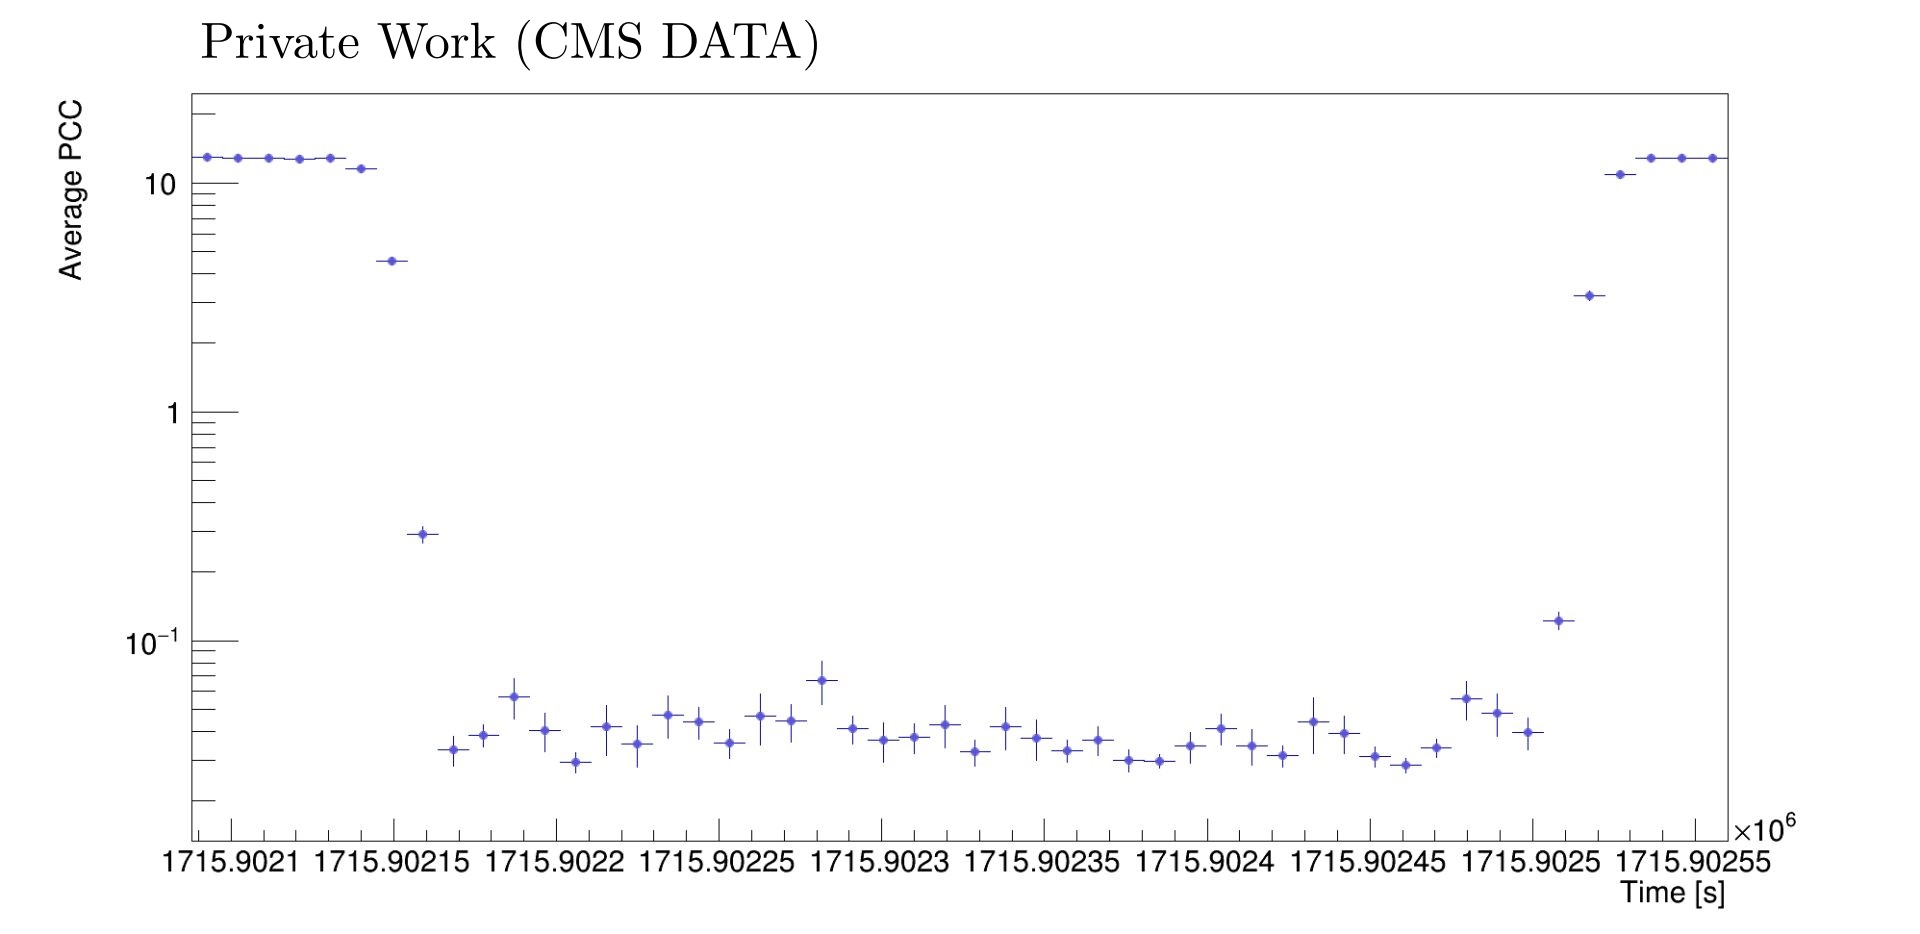
\includegraphics[width=1\textwidth]{SS1.jpeg}
    \caption{Histogram of rates during the second super separation scan}
    \label{fig:SS1}
\end{figure}

In the image we can see that the average rate suddenly drops, this is the beggining of the second super separation scan for the bcid 506 where the avarage rate drop but is non zero, then the rate goes up again meaning the end to the super separation scan.  

\section{Background Estimation}

The background estimation is obtained during the super separation (SS) process, since the SS scan separates the beams so they shouldn't be colliding the expected value on the rate is expected to be a rate associated with the background, this is then estimated by checking each of the SS scans on the time window referred on the table (3.1), the mean value during this period is assumed to be the mean value of the SS period, in the following table we see the mean PCC value for each period.  

\begin{table} [H]
\begin{center}
\caption{Different Scans}
\begin{tabular}{|c c c|} 
 \hline
 Scan & Mean & std  \\ [0.5ex] 
 \hline\hline
 SS1 &  & 1715883481  \\ 
 \hline
 SS2 &  & 1715902484  \\
 \hline
 SS3 &  & 1715919463 \\
 \hline
 SS6 &  & 1715943343  \\
 \hline
 SS5 &  & 1715987602  \\ [1.0ex]
 \hline
\end{tabular}
\end{center}
\end{table}

This is the mean value of each super separation off al the bcids a total of 60 mean values were obtained 


\section{Corrections}

\section{Fit model} 

There are different fit models at the time to do the vdm calibration, the most common one is Single Gaussian but also other models like the Double Gaussian, QG, Poly2g or Poly 4G. Each of these models have different parameters and restrictions making some of them better than other on the fit quality. 


\section{Beam Parameters}




	\chapter{Run 2 Luminosity Measurement}  %Title of the First Chapter

\ifpdf
    \graphicspath{{Chapter4/Figs/Raster/}{Chapter4/Figs/PDF/}{Chapter4/Figs/}}
\else
    \graphicspath{{Chapter4/Figs/Vector/}{Chapter4/Figs/}}
\fi

%\section{Methodology}
%\label{sec:method}

%Chapter 4: Run 2 Luminosity Measurement 

%Detector Module selection
%Afterglow Model
%vdM Calibration Results
%Luminosity for Physics Fills
%Systematic Uncertainties

\section{Dataset}

For studying the performance of PCC luminometer during 2018 data taking, we have divided CMS luminosity data taking into seven periods: A, B, C, D1, D2, D3, and D4, as depicted in % 2018 CMS luminosity data taking is divided into seven periods namely A, B, C, D1, D2, D3 and D4
Fig. \ref{fig:period_bound}. Run ranges for each period are shown in Table \ref{tab:period_run_ranges}.
During period B, specifically corresponding to Fill 6868, van der Meer (vdM) scans were conducted for calibrating the PCC luminometer.
%vdM data is shown during period B corresponding to Fill 6868.

\begin{figure}[!htp]
\centering
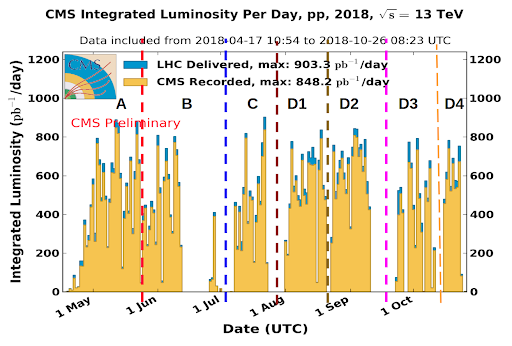
\includegraphics[width=0.9\textwidth]{ashish_thesis/period_boundary.png}
\caption[2018 CMS Luminosity Data Period]{%
   2018 luminosity data taking periods showing data taking period boundaries and vdM calibration data (1 July in period B)  \cite{CERNLumiPublicResults}.
}
\label{fig:period_bound}
\end{figure}


\begin{table}
  \begin{center}
    \caption[Run ranges for 2022 periods]{2018 luminosity data periods with run ranges.}
    \begin{tabular}{ccccc}
    \textbf{Period}   & \textbf{Run range} \\ \hline
     2018A      &        315252-316995         \\
     2018B      &        317080-319311         \\
     2018C      &        319337-320065         \\
     2018D1     &        320500-321665        \\
     2018D2     &        321710-322964         \\
     2018D3     &        323363-324420         \\
     2018D4     &        324564-325175        \\
      \end{tabular}
    %\caption[Run ranges]{2018 luminosity data periods with run ranges.}
    \label{tab:period_run_ranges}
  \end{center}
\end{table}

In the study under consideration, the datasets have been drawn from the Alignment and Calibration (AlCa) project, an integral component of the CMS experiment. The dataset selection includes two subsets: Random trigger and Zero-Bias. The Random trigger dataset comprises of data where trigger is applied on both colliding and non-colliding bunches. On the other hand, the Zero-Bias dataset encapsulates events that have passed the trigger system with no bias which means the colliding bunches are randomly triggered without the use of any CMS detector signal. The list of colliding bunches is detected by an independent system Beam Pick-up Timing system (BPTX) for Experiments. CMS software (CMSSW) version $10{\_}2{\_}2$ is used for reprocessing random trigger PCC dataset and $10{\_}6{\_}30$  \cite{CMSReleaseNotes} is used for reprocessing zero bias PCC datasets.

\begin{comment}
  
\begin{table}[htbp]
  \centering
  \begin{tabular}{@{}c@{\hspace{0.5cm}}p{6.5cm}p{6.5cm}@{}}
    \textbf{Period} & \textbf{Random Trigger Dataset} & \textbf{Zero Bias Dataset} \\
    2018A & /AlCaLumiPixels/Run2018A-\newline AlCaPCCRandom-15Apr2023\_UL2018\_\newline 315252\_316062\_PCCRandom\_-v1/ALCARECO, \newline /StreamALCALUMIPIXELSEXPRESS/\newline Run2018A-AlCaPCCRandom-Express-v1/ALCARECO & /AlCaLumiPixels/Run2018A-\newline AlCaPCCZeroBias-\newline 13Mar2023\_UL2018\_PCC-v1/ALCARECO \\
    2018B & /StreamALCALUMIPIXELSEXPRESS/\newline Run2018B-AlCaPCCRandom-Express-v1/ALCARECO & /AlCaLumiPixels/Run2018B-\newline AlCaPCCZeroBias-\newline 13Mar2023\_UL2018\_PCC-v1/ALCARECO \\
    2018C & /StreamALCALUMIPIXELSEXPRESS/\newline Run2018C-AlCaPCCRandom-Express-v1/ALCARECO & /AlCaLumiPixels/Run2018C-\newline AlCaPCCZeroBias-\newline 13Mar2023\_UL2018\_PCC-v1/ALCARECO \\
    2018D & /StreamALCALUMIPIXELSEXPRESS/\newline Run2018D-AlCaPCCRandom-Express-v1/ALCARECO & /AlCaLumiPixels/Run2018D-\newline AlCaPCCZeroBias-\newline 13Mar2023\_UL2018\_PCC-v1/ALCARECO \\
  \end{tabular}
  \caption[PCC datasets]{Datasets used for studying performance of PCC luminometer \cite{CERNDAS}}
  \label{tab:datasets}
\end{table}

\begin{table}[htbp]
  \centering
  \begin{tabular}{@{}c@{\hspace{0.5cm}}p{6.5cm}p{6.5cm}@{}}
    \textbf{Period} & \textbf{Random Trigger Dataset} & \textbf{Zero Bias Dataset} \\[1em]
    2018A & /AlCaLumiPixels/Run2018A-\newline AlCaPCCRandom-15Apr2023\_UL2018\_\newline 315252\_316062\_PCCRandom\_-v1/ALCARECO, \newline /StreamALCALUMIPIXELSEXPRESS/\newline Run2018A-AlCaPCCRandom-Express-v1/ALCARECO & /AlCaLumiPixels/Run2018A-\newline AlCaPCCZeroBias-\newline 13Mar2023\_UL2018\_PCC-v1/ALCARECO \\[1em]
    2018B & /StreamALCALUMIPIXELSEXPRESS/\newline Run2018B-AlCaPCCRandom-Express-v1/ALCARECO & /AlCaLumiPixels/Run2018B-\newline AlCaPCCZeroBias-\newline 13Mar2023\_UL2018\_PCC-v1/ALCARECO \\[1em]
    2018C & /StreamALCALUMIPIXELSEXPRESS/\newline Run2018C-AlCaPCCRandom-Express-v1/ALCARECO & /AlCaLumiPixels/Run2018C-\newline AlCaPCCZeroBias-\newline 13Mar2023\_UL2018\_PCC-v1/ALCARECO \\[1em]
    2018D & /StreamALCALUMIPIXELSEXPRESS/\newline Run2018D-AlCaPCCRandom-Express-v1/ALCARECO & /AlCaLumiPixels/Run2018D-\newline AlCaPCCZeroBias-\newline 13Mar2023\_UL2018\_PCC-v1/ALCARECO \\[1em]
  \end{tabular}
  \caption{Datasets used for studying performance of PCC luminometer}
  \label{tab:datasets}
\end{table}


\begin{table}[htbp]
  \centering
  \begin{tabular}{@{}c@{\hspace{1cm}}p{5.5cm}p{5.5cm}@{}}
    \textbf{Period} & \textbf{Random Trigger Dataset} & \textbf{Zero Bias Dataset} \\
    2018A & \begin{tabular}{@{}p{5.5cm}@{}}/AlCaLumiPixels/Run2018A-AlCaPCCRandom-15Apr2023\_UL2018\_315252\_316062\_PCCRandom\_-v1/ALCARECO, \\ /StreamALCALUMIPIXELSEXPRESS/Run2018A-AlCaPCCRandom-Express-v1/ALCARECO\end{tabular} & /AlCaLumiPixels/Run2018A-AlCaPCCZeroBias-13Mar2023\_UL2018\_PCC-v1/ALCARECO \\
    2018B & /StreamALCALUMIPIXELSEXPRESS/Run2018B-AlCaPCCRandom-Express-v1/ALCARECO & /AlCaLumiPixels/Run2018B-AlCaPCCZeroBias-13Mar2023\_UL2018\_PCC-v1/ALCARECO \\
    2018C & /StreamALCALUMIPIXELSEXPRESS/Run2018C-AlCaPCCRandom-Express-v1/ALCARECO & /AlCaLumiPixels/Run2018C-AlCaPCCZeroBias-13Mar2023\_UL2018\_PCC-v1/ALCARECO \\
    2018D & /StreamALCALUMIPIXELSEXPRESS/Run2018D-AlCaPCCRandom-Express-v1/ALCARECO & /AlCaLumiPixels/Run2018D-AlCaPCCZeroBias-13Mar2023_UL2018_PCC-v1/ALCARECO \\
  \end{tabular}
  \caption{Datasets used for studying performance of PCC luminometer}
  \label{tab:datasets}
\end{table}

\end{comment}

\begin{comment}

The calibration of luminosity measurement by the CMS experiment luminometers in the 2018 proton-proton data taking at $\sqrt{s}$ = 13 TeV \cite{CMS-PAS-LUM-18-002} was performed during LHC fill 6868 on June 30 and July 1, 2018 at $\sqrt{s}$ = 13 TeV. Zero-bias triggers on 5 bunch pairs (BCIDs 265, 865, 1780, 2192, and 3380) recorded events rate is 27.7 kHz. Trigger is applied on five colliding bunches due to limitation of the recording bandwidth. 

%\item "lsc1", was the "constant separation" scan, two beams were separated by 1.4 $\sigma$ and moved together in steps of 1 $\sigma$ across and back.
%\item "lsc2", was the "variable separation" scan method, one beam (starting with beam 1) is moved to -2.5 $\sigma$ and then a three-point scan (a "miniscan") is performed with the other beam.
%a normal VdM scan pair "norm4" and two short emittance scan pairs "emit4" and "emit5" were also performed.

%The 2018 CMS VdM scan program was conducted in two segments, interrupted by an alarm. The first segment involved six x-y scan pairs. Two were short ``emittance'' scans, named ``emit1'' and ``emit2,'' where the beams were separated by $ \(4\sigma_b\) $ over 9 steps with a 10 second integration time at each step. A standard VdM scan, named ``norm1,'' separated the beams by $\(6\sigma_b \approx 600\)~\mu m$ in 25 steps, with a 30-second duration per step. The ``offset1'' scan followed the same procedure as the standard scans but with a $\(\pm 1.5\sigma_b\)$ separation in the non-scanning direction. Lastly, two sets of ``beam imaging'' scans were conducted, where one beam remained fixed while the other was moved in 19 steps between $\(+4.5\sigma_b\)$ and $\(-4.5\sigma_b\)$, each lasting 46 seconds per step.

The 2018 CMS VdM scan program (shown in Fig. \ref{fig:vdm_prog_2018}) was conducted in two segments, interrupted by an alarm. The first segment involved six x-y scan pairs. Two were short ``emittance'' scans, named ``emit1'' and ``emit2,'' where the beams were separated by \(4\sigma_b\) over 9 steps with a 10-second integration time at each step. A standard vdM scan (described in section 3.1), named ``norm1,'' separated the beams by \(6\sigma_b \approx 600\)~$\mu$m in 25 steps, with a 30-second duration per step. The ``offset1'' scan followed the same procedure as the standard scans but with a \(\pm 1.5\sigma_b\) separation in the non-scanning direction. Lastly, two sets of ``beam imaging'' scans were conducted, where one beam remained fixed while the other was moved in 19 steps between \(+4.5\sigma_b\) and \(-4.5\sigma_b\), each lasting 46 seconds per step. The second part of the scan program was conducted in the same fill, approximately 7.5 hours later, and consisted of twelve scan pairs. This included a short emittance scan, ``emit3''; beam imaging scan pairs, ``imag2'' and ``imag3''; an offset scan pair, ``offset2''; and two standard VdM scan pairs, ``norm2'' and ``norm3''.

Beam Imaging Scans: Beam imaging scans are designed to measure the transverse profile of the beam. They involve moving one beam across the other in steps and measuring the interaction rate (or event rate) at each step. By doing this, the shape or "profile" of the beam in the transverse plane can be obtained. These scans allow for a detailed analysis of the beam shape, which is essential for understanding the beam properties. In a perfect scenario, the density distributions of protons in a bunch would factorize into separate X (horizontal) and Y (vertical) components. However, real beams can have correlations between X and Y (non-factorization). Beam imaging scans help map the 2D profile of the beam and are thus essential for diagnosing and understanding any such correlations. Knowing the 2D profile of the beams is crucial when calculating luminosity, as assumptions made about the factorization of the beam profiles feed into these calculations. By using beam imaging scans, experimenters can assess the validity of the factorization assumption or correct for any observed non-factorization.

Offset Scans: Offset scans are performed to check for systematic errors in the luminosity measurement, which may arise from various sources. They are similar to standard VdM scans but involve an intentional offset in the non-scanning direction. By comparing the results of offset scans with the results of regular scans, one can identify and correct for any systematic discrepancies that are present. Offset scans can help to assess the sensitivity of the luminosity measurement to non-factorization in the transverse plane. For example, if there are correlations between the X and Y distributions of protons (i.e., non-factorization), this could in principle affect the shape of the beam overlap region in the collision point. Offset scans, by changing the relative position of the beams, can help to assess whether such non-factorization has a significant effect on the measured luminosity.

%The second part of the scan program was conducted in the same fill, approximately 7.5 hours later, and consisted of twelve scan pairs. This included a short emittance scan, ``emit3''; beam imaging scan pairs, ``imag2'' and ``imag3''; an offset scan pair, ``offset2''; and two standard VdM scan pairs, ``norm2'' and ``norm3''.

vdM scans are typically conducted at least once a year to ensure the luminometer is correctly calibrated. Results of these scans that is the visible cross section is used to normalize the data collected by the experiments during physics run.

\begin{figure}[h]
    \centering
    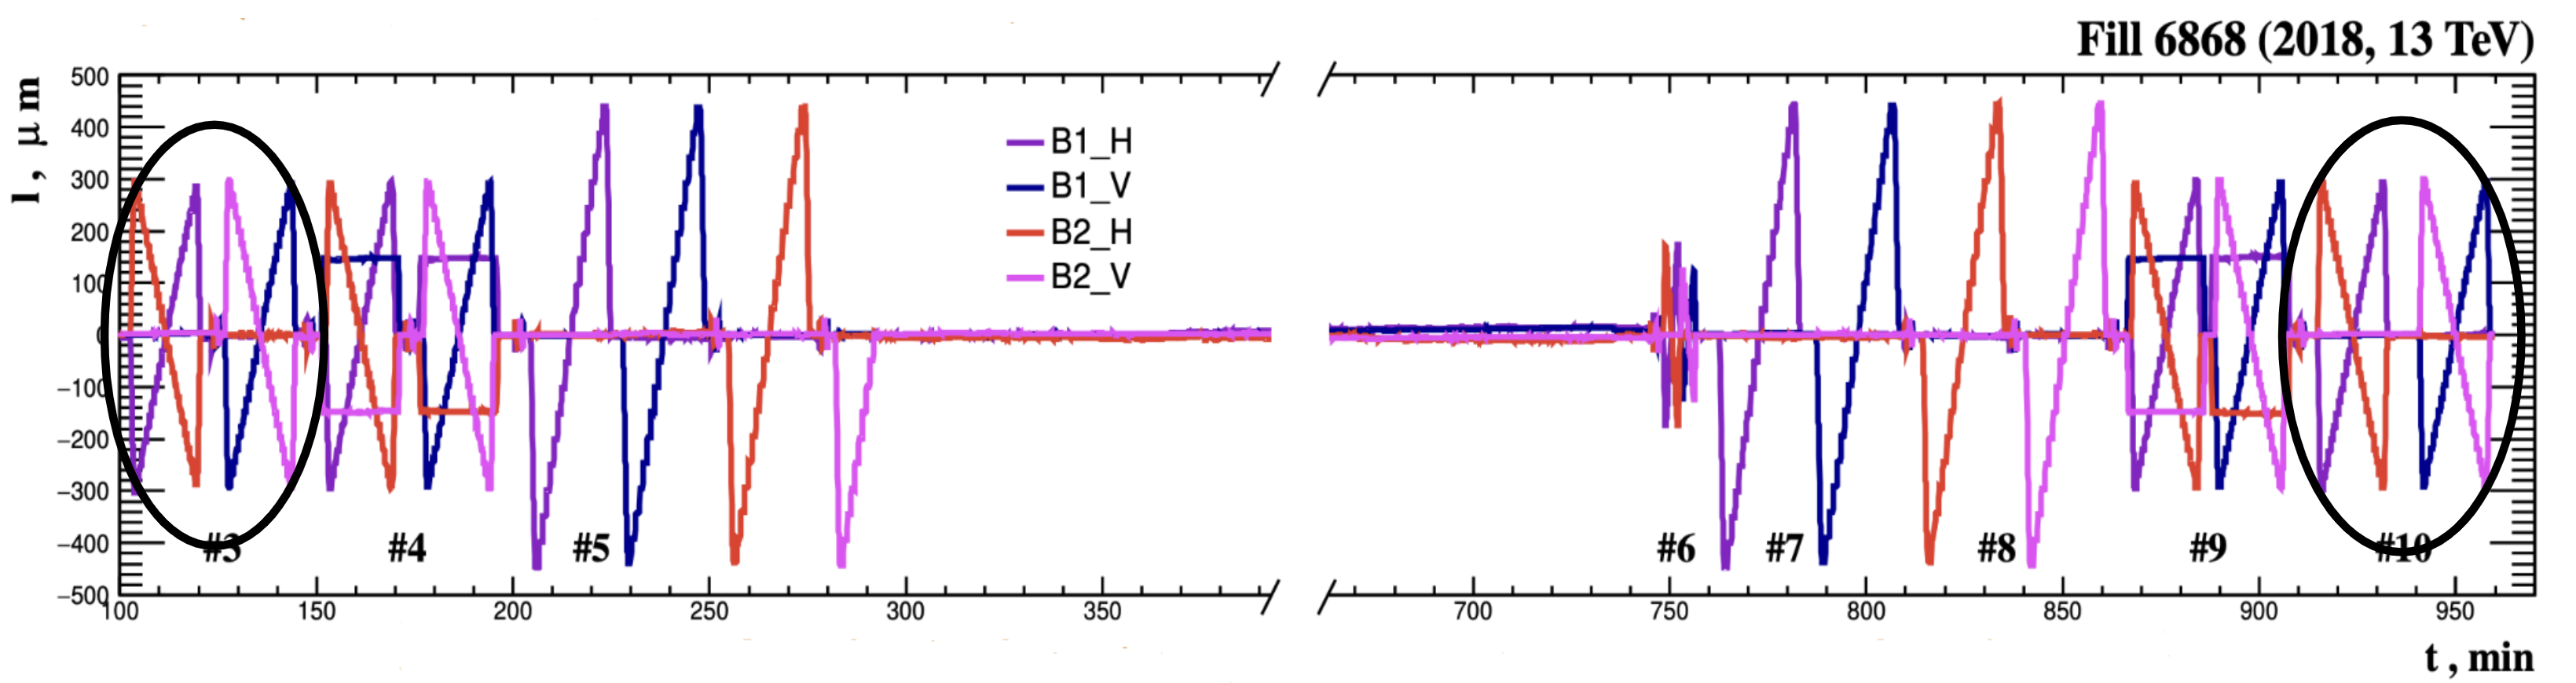
\includegraphics[width=1\textwidth]{ashish_thesis/vdm_program_2018.png}
    \caption[2018 vdM program]{Beam position along x and y is plotted as a function of time showing different types of scans. #3 and #10 are vdM scans, #4 and #9 are offset scans, #5, #7 and #8 are beam imaging scans, #6 is emittance scan.
}
    \label{fig:vdm_prog_2018}
\end{figure}

\end{comment}

%In order to measure luminosity using a pixel detector, the count of pixel clusters is studied for each module, with each module being composed of numerous pixels arranged in a grid. The number of pixel clusters recorded per unit time in each module is proportional to the instantaneous luminosity of the collider. The Pixel Cluster Counting (PCC) method is implemented by operating the pixel detector in an integrated mode. The Pixel detector is read out at a fixed interval termed a "lumi section", each lasting for 23.36 seconds.

The pixel detector records data for each bunch-crossing, though the readout rate is constrained by the trigger. During subsequent data processing,  these events are consolidated into lumi sections. During each lumi section, the number of pixel clusters produced in each module is recorded and the module weights for all pixel modules are studied to track their performance over time. This helps in identifying good and bad modules, as shown in Fig. \ref{fig:goodbadmodules}. Only pixel modules that demonstrate consistent and reliable performance throughout the entire 2018 year are considered good and included in the analysis. The pixel cluster rate, along with the visible cross section of the detector, is used to determine the instantaneous luminosity of the collider. PCC data is subsequently reprocessed. This involves the re-analysis of the data using updated or refined algorithms, calibrations, and detector conditions.

%To measure the luminosity using the pixel detector, pixel cluster count is studied for each module, where a module consists of a number of pixels arranged in a grid. The number of pixel clusters recorded in each module per unit time is proportional to the instantaneous luminosity of the collider. To implement PCC method, the pixel detector is operated in an integrated mode, where the detector is read out at a fixed time interval called a "lumi section". During each lumi section, the number of pixel clusters produced in each module is recorded, the rate of pixel clusters and visible cross section of the detector is used to determine the instantaneous luminosity of the collider. PCC data is reprocessed, a procedure that involves the re-analysis of the data using refined or updated algorithms, calibrations, or detector conditions.

The purpose of reprocessing can be multifold:

\begin{itemize}
  
\item Improved Algorithms or Calibration: As experiments progress, there can be improvements in algorithms or calibration techniques used to process the raw data. This can lead to a more accurate or efficient representation of the collected data.

\item Changes in Detector Conditions: Detector conditions might change over time due to factors like aging or upgrades. These changes can affect the interpretation of the data.

\item Discovery of Issues or Errors: Sometimes, errors or issues in the original data processing might be discovered.

\end{itemize}
  
In the context of PCC data, reprocessing can lead to a more accurate luminosity measurement, which in turn can affect the interpretation of the physics results derived from the LHC data. Random trigger PCC dataset is reprocessed with new module veto list (described in section 4.2) to obtain afterglow corrections with improved module stability selections. Zero-bias dataset is reprocessed after applying afterglow corrections using same module veto list with more stringent selections on module stability to obtain PCC luminosity.

%CMS software (CMSSW) version $10{\_}2{\_}2$ is used for reprocessing random trigger PCC dataset and $10{\_}6{\_}30$  \cite{CMSReleaseNotes} is used for reprocessing zero bias PCC datasets. %Datasets can be obtained by applying triggers on all bunches (colliding and non colliding) and only on colliding bunches to get random trigger and zero bias data respectively as described in previous section.
%Random trigger PCC dataset is reprocessed with new module veto list (described in section 4.2) to obtain afterglow corrections with improved module stability selections. Zero-bias dataset is reprocessed after applying afterglow corrections using same module veto list with more stringent selections on module stability to obtain PCC luminosity. 
%To ensure accurate luminosity measurements, it is necessary to correct for various effects, such as detector inefficiencies and pileup (the presence of additional proton-proton collisions in the same bunch crossing). This is achieved through careful calibration of the detector and by using dedicated algorithms to estimate the contribution of pileup to the observed pixel cluster counts.

\begin{comment}

\begin{table}
  \begin{center}
    \begin{tabular}{ccccc}  
    \textbf{Period}   & \textbf{Run range} \\ \hline
     2018A      &        315252-316995         \\ 
     2018B      &        317080-319311         \\ 
     2018C      &        319337-320065         \\ 
     2018D1     &        320500-321665        \\ 
     2018D2     &        321710-322964         \\ 
     2018D3     &        323363-324420         \\ 
     2018D4     &        324564-325175        \\ 
      \end{tabular}
    \caption{2018 luminosity data periods with run ranges.}
    \label{tab:period run ranges}
  \end{center}
\end{table}

\section{Software tools}

%CERN ROOT is a software framework commonly used in particle physics to analyze large datasets generated by particle detectors such as the CMS experiment at CERN. One of the important measurements performed at CMS is the determination of the instantaneous luminosity, which is a measure of the rate at which particles are colliding in the detector. To measure the luminosity at CMS, the detector records signals from various sub-detectors, such as the silicon tracker and the calorimeters, which are used to reconstruct the tracks and energy deposits of particles produced in the collisions. These signals are then processed using the CERN ROOT framework to extract relevant information such as the number of collisions per second and the total integrated luminosity over a given period of time.The CERN ROOT framework is used to analyze the data from van der Meer scans and extract the luminosity calibration factors needed to convert the collision rates into actual luminosity measurements. To extract Pixel Cluster Counting (PCC) datasets from the CMS Data Aggregation Service (DAS) using a shell script, we can use the dasgoclient command-line tool. For example, following command can copy names of all root files into a text file.
 
%\begin{verbatim}
 % dasgoclient -query="file dataset=/AlCaLumiPixels/Run2018A-AlCaPCCZeroBias- 27Oct2022_UL2018_PCC-v1/ALCARECO instance=prod/global | grep file.name | grep  '.root'" > Run2018A.txt   
%\end{verbatim}

%\begin{itemize}
    
%\item  In the CMS experiment at CERN, luminosity measurements using the Pixel Cluster Counting (PCC) method are typically performed using the CMSSW framework. The luminosity module and configuration files used in CMSSW to perform PCC luminosity measurements can be generated using C++ code and Python scripts. 

%\item  HTCondor is used to process PCC datasets, is a high-throughput computing (HTC) system that can be used to submits jobs for each run to efficiently manage large-scale data processing tasks, such as those required in the analysis of data from high-energy physics experiments. HTCondor provides a framework for distributing and managing the processing of this data across a large number of computing nodes. This allows the luminosity measurement to be performed more quickly and efficiently than would be possible using a traditional computing approach. Specifically, 

%\item HTCondor is used to manage the processing of so-called "luminosity blocks" of data, which correspond to periods of time during which the accelerator was operating at a certain luminosity. These blocks can contain many terabytes of data, and processing them requires significant computing resources. With HTCondor, the processing of these blocks can be distributed across a large number of computing nodes, allowing the analysis to be performed in parallel. Additionally, HTCondor provides features for managing the scheduling of jobs and ensuring that data is transferred between nodes efficiently, which is critical for achieving high throughput in the analysis.

%\end{itemize}

\begin{itemize}

\item CMSSW: The CMS Software (CMSSW) is a comprehensive software framework developed for the Compact Muon Solenoid (CMS) experiment at the Large Hadron Collider (LHC) at CERN. CMSSW is used for the simulation, processing, and analysis of data collected by the CMS detector. It is designed to handle various tasks, from the generation of simulated events to the reconstruction of raw detector data, calibration, and high-level analysis. CMSSW is composed of several interconnected components and follows a modular architecture to promote flexibility, reusability, and maintainability. Some key aspects of CMSSW include, Event Data Model (EDM): The EDM serves as the foundation of CMSSW, defining the structure and organization of data objects, such as particle candidates, detector hits, and reconstructed vertices. It is designed to handle the storage, retrieval, and manipulation of these objects efficiently. The CMSSW framework is responsible for the management of software modules, the flow of data between modules, and the execution of the necessary tasks. It also handles the scheduling of tasks and the parallelization of processes, enabling efficient use of computing resources. Modules: CMSSW is built upon a collection of software modules, each responsible for a specific task, such as event generation, detector simulation, reconstruction, or analysis. These modules can be combined and customized to create a complete processing chain for a given use case. The software includes a detailed description of the CMS detector geometry, material properties, and readout electronics. This information is used during the simulation and reconstruction processes to accurately model the detector's response to particles. 
Simulation: CMSSW integrates several external tools and libraries, such as the GEANT4 toolkit, to simulate the passage of particles through the CMS detector. This includes the interactions of particles with the detector material, the production of secondary particles, and the generation of detector signals. Reconstruction: The reconstruction algorithms in CMSSW process the raw detector data, converting it into meaningful physics objects, such as tracks, calorimeter clusters, and particle candidates. These algorithms use a variety of techniques, including pattern recognition, clustering, and fitting, to extract the relevant information from the detector signals. CMSSW includes tools for the calibration of detector components and the alignment of the detector geometry. These tasks are crucial for ensuring the accurate reconstruction of physics objects and the extraction of meaningful results from the data. Analysis: The software provides a rich set of high-level analysis tools and libraries, enabling researchers to perform a wide range of physics analyses, from searches for new particles to precision measurements of Standard Model processes. Data storage and management: CMSSW uses the ROOT data format for the storage and management of data objects. ROOT is a powerful and flexible data storage and processing framework developed at CERN, which provides efficient data handling, advanced statistical analysis tools, and extensive data visualization capabilities \cite{CMSWorkBook}.

\item Conditions Database (CondDB): The Conditions Database (CondDB) is a centralized data storage and management system used in high-energy physics experiments, such as the Compact Muon Solenoid (CMS) at the Large Hadron Collider (LHC) at CERN. The primary purpose of CondDB is to store non-event-related data, known as "conditions data," which is essential for the proper interpretation and analysis of the experimental data. Conditions data includes information on the detector's configuration, calibration constants, alignment parameters, and other time-dependent data that characterize the performance and status of the detector and its components. Since the conditions data is critical for accurate data processing and analysis, it must be readily accessible and easily managed. CondDB provides a central repository for storing conditions data from various sources, such as detector control systems, calibration measurements, and offline analyses. This centralization simplifies data management and ensures that all data processing tasks have access to the same, consistent information. Time-dependent data management: The database is designed to handle time-dependent data efficiently. Each data record stored in CondDB is associated with a specific time interval, known as the "IOV" (Interval of Validity). This enables the retrieval of the correct conditions data corresponding to a specific data-taking period. Data versioning: CondDB supports versioning of the conditions data, allowing researchers to track changes and updates to the data over time. This feature ensures reproducibility of results and facilitates comparisons between different data processing and analysis workflows. Access control: The database provides fine-grained access control mechanisms, enabling authorized users to read, write, and modify conditions data. This ensures the integrity of the data and prevents unauthorized modifications. CondDB is designed to handle the large volume of conditions data generated by high-energy physics experiments, with efficient data storage and retrieval mechanisms. The database is built on robust and scalable technologies, such as relational databases (e.g., Oracle, MySQL, or PostgreSQL), to ensure high performance and reliability. Integration with data processing frameworks: The Conditions Database is designed to integrate seamlessly with data processing and analysis frameworks, such as the CMS Software (CMSSW). This integration allows for the automatic retrieval and usage of conditions data during the data processing workflow, ensuring the correct data is used at each step of the process.

\item HTCondor: HTCondor is a specialized workload management system designed for distributed computing environments. Developed at the University of Wisconsin-Madison, HTCondor is an open-source system that facilitates the efficient utilization of computing resources by managing and scheduling compute jobs across a network of computers. It is widely used in various scientific domains, including high-energy physics, bioinformatics, and computer science, to handle large-scale computational tasks. HTCondor is designed to discover, monitor, and manage a heterogeneous collection of computing resources, including desktop computers, dedicated clusters, and cloud computing resources. It can efficiently allocate jobs to resources based on the requirements of the jobs and the availability of the resources. HTCondor provides a sophisticated job scheduling system, which prioritizes and assigns jobs to appropriate resources based on various criteria, such as resource availability, job requirements, and user-defined policies. The scheduler supports various scheduling strategies, including fair-sharing, priority-based, and opportunistic scheduling. HTCondor is designed to be fault-tolerant and can automatically recover from failures or interruptions in the computing environment. In case a job fails to complete due to a system crash or network disconnection, HTCondor can reschedule the job to another available resource, ensuring that the job eventually completes. Data management: HTCondor provides built-in data management capabilities, allowing users to transfer input and output files between the submitting machine and the executing machines. This feature simplifies data handling in distributed computing environments and ensures that jobs have access to the required data. HTCondor provides a range of security mechanisms to protect the integrity and confidentiality of both the jobs and the computing resources. These mechanisms include authentication, authorization, data encryption, and sandboxing, which prevent unauthorized access and tampering. HTCondor enables users to monitor the progress of their jobs, providing information on job status, resource usage, and performance. Users can also control their jobs by pausing, resuming, or canceling them as needed. Interoperability and extensibility: HTCondor is designed to interoperate with other computing systems and can be easily integrated into existing workflows. It supports various job submission languages, such as the Job Submission Description Language (JSDL) and the ClassAd language, and can be extended with custom plugins and scripts. HTCondor is compatible with a wide range of operating systems, including Linux, macOS, and Windows, enabling users to harness the full potential of their computing resources, regardless of the underlying platform.

\item CMS Data Aggregation System (DAS): The CMS Data Aggregation System (DAS) is a data management tool designed for the Compact Muon Solenoid (CMS) experiment at the Large Hadron Collider (LHC) at CERN. It serves as a centralized query system that simplifies the process of locating and accessing various types of CMS data and metadata. DAS aggregates information from multiple data services and presents it in a unified manner, enabling researchers to easily search for and retrieve the data they need for their analyses. DAS provides a unified query language that allows users to perform searches across different data services using a single, consistent syntax. This simplifies the process of data discovery and reduces the learning curve associated with using multiple data services. DAS is designed to aggregate data from various data services within the CMS experiment, including data storage systems, data catalogs, and data processing services. By consolidating this information, DAS enables researchers to easily search for and access the data they need, without having to interact with multiple data services individually. Data caching: To improve performance and reduce the load on the underlying data services, DAS employs a caching mechanism that temporarily stores the results of previous queries. This allows DAS to quickly return results for frequently requested queries, without having to query the data services each time. DAS can merge data from multiple sources, providing users with a consolidated view of the information. This feature simplifies data analysis by eliminating the need for researchers to manually merge data from different sources. DAS supports data transformation operations, such as filtering, sorting, and aggregation, allowing users to customize the output of their queries to meet their specific needs. This feature helps researchers focus on the most relevant information and reduces the amount of data they need to process. DAS is designed to be extensible, enabling the integration of additional data services as needed. This allows DAS to adapt to the evolving needs of the CMS experiment and continue to provide a unified interface for data discovery and access. DAS offers a web-based user interface that allows users to submit queries and view the results using a standard web browser. This makes it easy for researchers to access and use the system, regardless of their location or computing environment. API access: In addition to the web-based user interface, DAS provides an Application Programming Interface (API) that allows users to programmatically submit queries and retrieve results. This enables the integration of DAS with other software tools and workflows used by the CMS experiment.

\item Brilcalc: The brilcalc tool is a software package designed to calculate and analyze luminosity data for the Compact Muon Solenoid (CMS) experiment at the Large Hadron Collider (LHC) at CERN. Luminosity is a crucial parameter in high-energy physics experiments like CMS, as it measures the rate of collisions in a particle accelerator and directly affects the statistical significance of experimental results. Brilcalc serves as a command-line interface (CLI) tool, which allows users to extract, manipulate, and visualize luminosity data from the CMS experiment. It is built upon the BRIL (Beam Radiation Instrumentation and Luminosity) project, which is responsible for the development and maintenance of beam monitoring and luminosity measurement systems at the CMS experiment. Users can extract luminosity data for a specific data-taking period or data range from the CMS database. The data can be filtered by various criteria, such as run number, fill number, and data-taking conditions. Data manipulation: The tool offers the capability to process and manipulate the extracted luminosity data. Users can perform operations such as unit conversion, data scaling, and data normalization to make the data suitable for further analysis. Brilcalc allows users to perform basic statistical analyses on the luminosity data, such as calculating integrated luminosity, average luminosity, and instantaneous luminosity. These analyses help physicists understand the performance of the CMS detector and plan future data-taking strategies. The tool can generate plots and graphs to visualize the luminosity data, making it easier for researchers to interpret the results and identify trends or anomalies. Brilcalc is designed to be extensible, allowing users to develop custom plugins and scripts for advanced data analysis and visualization tasks \cite{CMSLuminosityCalculationGuide}.

\item CERN ROOT: The ROOT data analysis framework, developed by CERN, is widely used in high-energy physics experiments, including CMS. ROOT offers a rich set of tools for data processing, statistical analysis, and visualization. In the context of PCC luminosity measurement, ROOT is employed to analyze and process the output data from CMSSW, perform statistical analyses, and generate plots for data visualization \cite{ROOT}.

\item Shell/Bash Scripting: Shell and bash scripting are widely used in high-energy physics research to automate repetitive tasks and manage workflows. These scripting languages offer flexibility and portability, allowing researchers to create custom scripts tailored to their specific needs. In the context of PCC luminosity measurement, shell/bash scripts are employed to streamline data processing, automate job submission to HTCondor, and manage the overall workflow, enhancing productivity and reducing the chances of human error.

\item DASgoclient: The DASgoclient is a command-line interface for the CMS Data Aggregation System (DAS). It offers researchers an alternative method for accessing various CMS data services without using the web-based DAS interface. The DASgoclient allows users to query and retrieve data in a more scriptable and automated manner, making it an essential tool for managing datasets and streamlining the data retrieval process for PCC luminosity measurement.

\end{itemize}

%\begin{figure}[!htp]
%\centering
%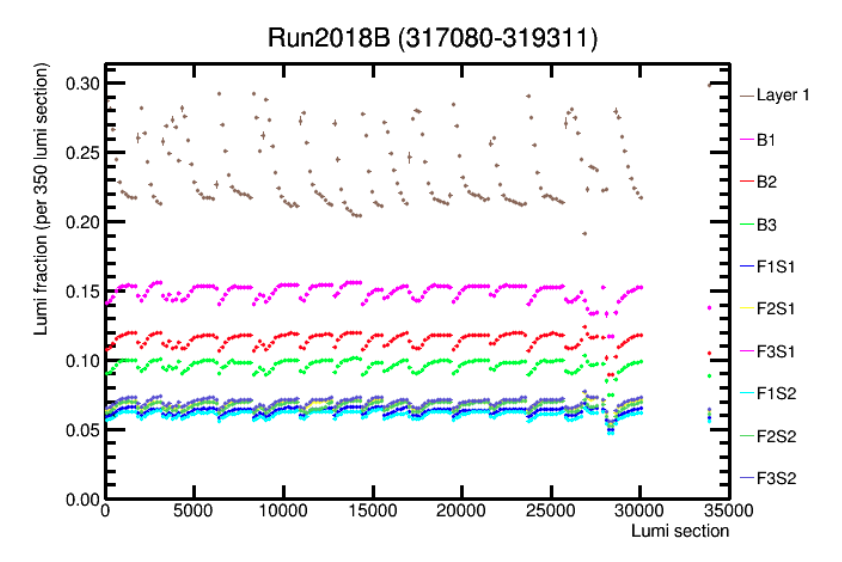
\includegraphics[width=0.8\textwidth]{ashish_thesis/pcc_stability_begin.png}
%\caption{%                                                                                                                                                                                          
 %  Luminosity fraction of pixel detector for various layer and disks as a function of lumi section after removing low statistics lumi section.
%}
%\label{fig:PCC_stab_begin}
%\end{figure}

%\begin{figure}[!htp]
%\centering
%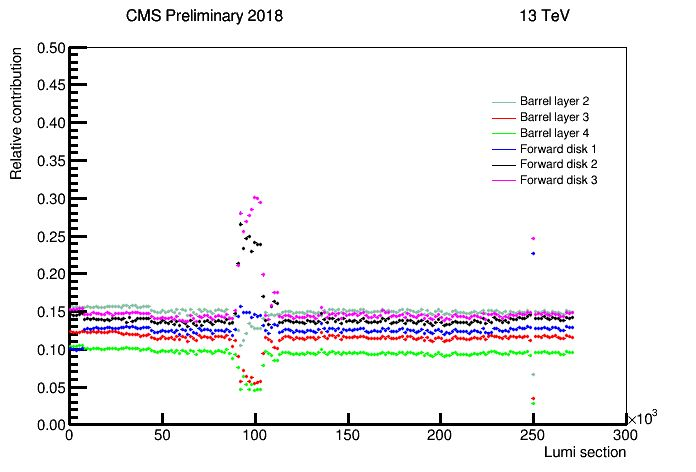
\includegraphics[width=0.8\textwidth]{ashish_thesis/pixel_layer_disk_noveto_noselection.png}
%\caption{%                                                                                                                                                                                                            
 %  Luminosity fraction of pixel detector for various layer and disks as a function of lumi section after removing low statistics lumi section.
%}
%\label{fig:PCC_stab_begin}
%\end{figure}


%\begin{figure}[!htp]
%\centering
%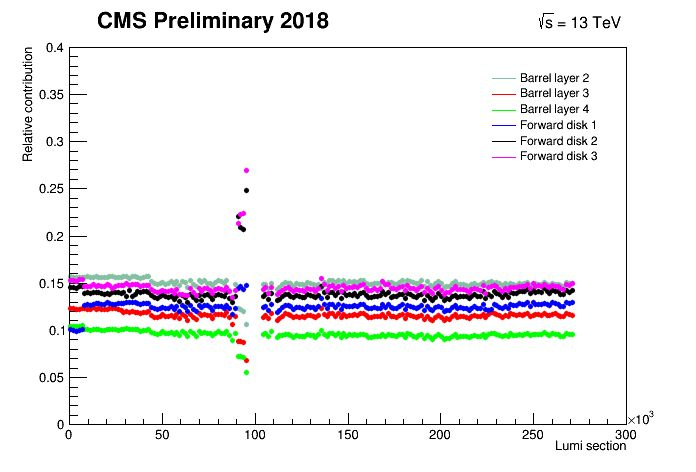
\includegraphics[width=0.8\textwidth]{ashish_thesis/pixel_layer_disk_noveto.png}
%\caption{%                                                                                                                                                                
 %  Luminosity fraction of pixel detector for various layer and disks as a function of lumi section after removing low statistics lumi section.
%}
%\label{fig:PCC_stab_begin}
%\end{figure}



%\begin{figure}[!htp]
%\centering
%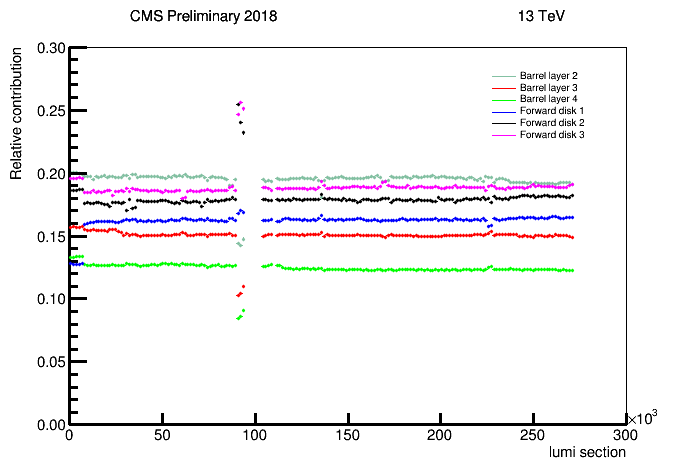
\includegraphics[width=0.8\textwidth]{ashish_thesis/pcc_frac_L0_veto.png}
%\caption{%                                                                                                                                                                           
 %  Luminosity fraction of pixel detector for various layer and disks as a function of lumi section after removing low statistics lumi section.
%}
%\label{fig:PCC_stab_L0_veto}
%\end{figure}


%\begin{figure}[!htp]
%\centering
%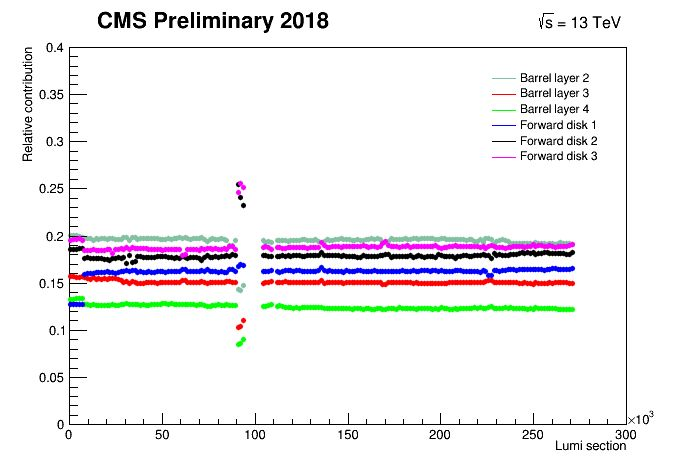
\includegraphics[width=0.8\textwidth]{ashish_thesis/pixel_layer_disk_B0_veto.png}
%\caption{%                                                                                                                                                                           
 %  Luminosity fraction of pixel detector for various layer and disks as a function of lumi section after removing low statistics lumi section and all modules in Layer 1.
%}
%\label{fig:PCC_stab_L0_veto}
%\end{figure}

\end{comment}


\section{Detector module selection}

The goal of minimizing instabilities in PCC luminosity measurement is to ensure precise and consistent results. To achieve this, a pixel module veto list is created for each period to keep track of  bad modules. The stability of each module is determined based on the change in the ratio of module PCC and total PCC, referred to as the module weight. %as shown in Fig. \ref{fig:mod_weight}.

%\begin{itemize}

%\item Lumi section duration: The data collected for luminosity measurements are divided into lumi sections, each lasting for 23.36 seconds.

%\item Analyzing module weights: During each lumi section, the module weights for all pixel modules are studied to track their performance over time. This helps in identifying good and bad modules, as shown in Fig. \ref{fig:goodbadmodules}.

%\item Pixel detector composition: The pixel detector used for the 2018 luminosity measurement comprises two main components - the BPIX (barrel pixel detector) with 4 barrel layers, and the FPIX (forward pixel detector) with three forward disks. These two components consist of 1184 and 672 pixel modules, respectively.

%\item Selection criteria: Only pixel modules that demonstrate consistent and reliable performance throughout the entire 2018 year are considered good and included in the analysis. %Modules that do not meet these criteria are classified as bad and excluded from the luminosity measurement.

%\end{itemize}

By carefully analyzing the module weights and excluding the bad modules from the analysis, the instabilities in PCC luminosity measurement can be minimized. This process ensures that the data used for luminosity measurement is of high quality and can produce precise results.

%To minimize instabilities in PCC luminosity measurement, pixel module vetolist is created for each run period. Module stability is based on change in the ratio of module PCC and total PCC which is defined as module weight. Change in module weights with lumi section (23.36s) is studied for all modules and used to select good and bad modules as shown in Fig. \ref{fig:goodbadmodules}. Pixel detector used for 2018 luminosity measurement consists of 4 barrel layers (BPIX) and three forward disks (FPIX) including 1184 and 672 pixel modules respectively. Only pixel modules that are found to show good performance during the entire 2018 year are selected. 

%\begin{figure}[!htp]
%\centering
%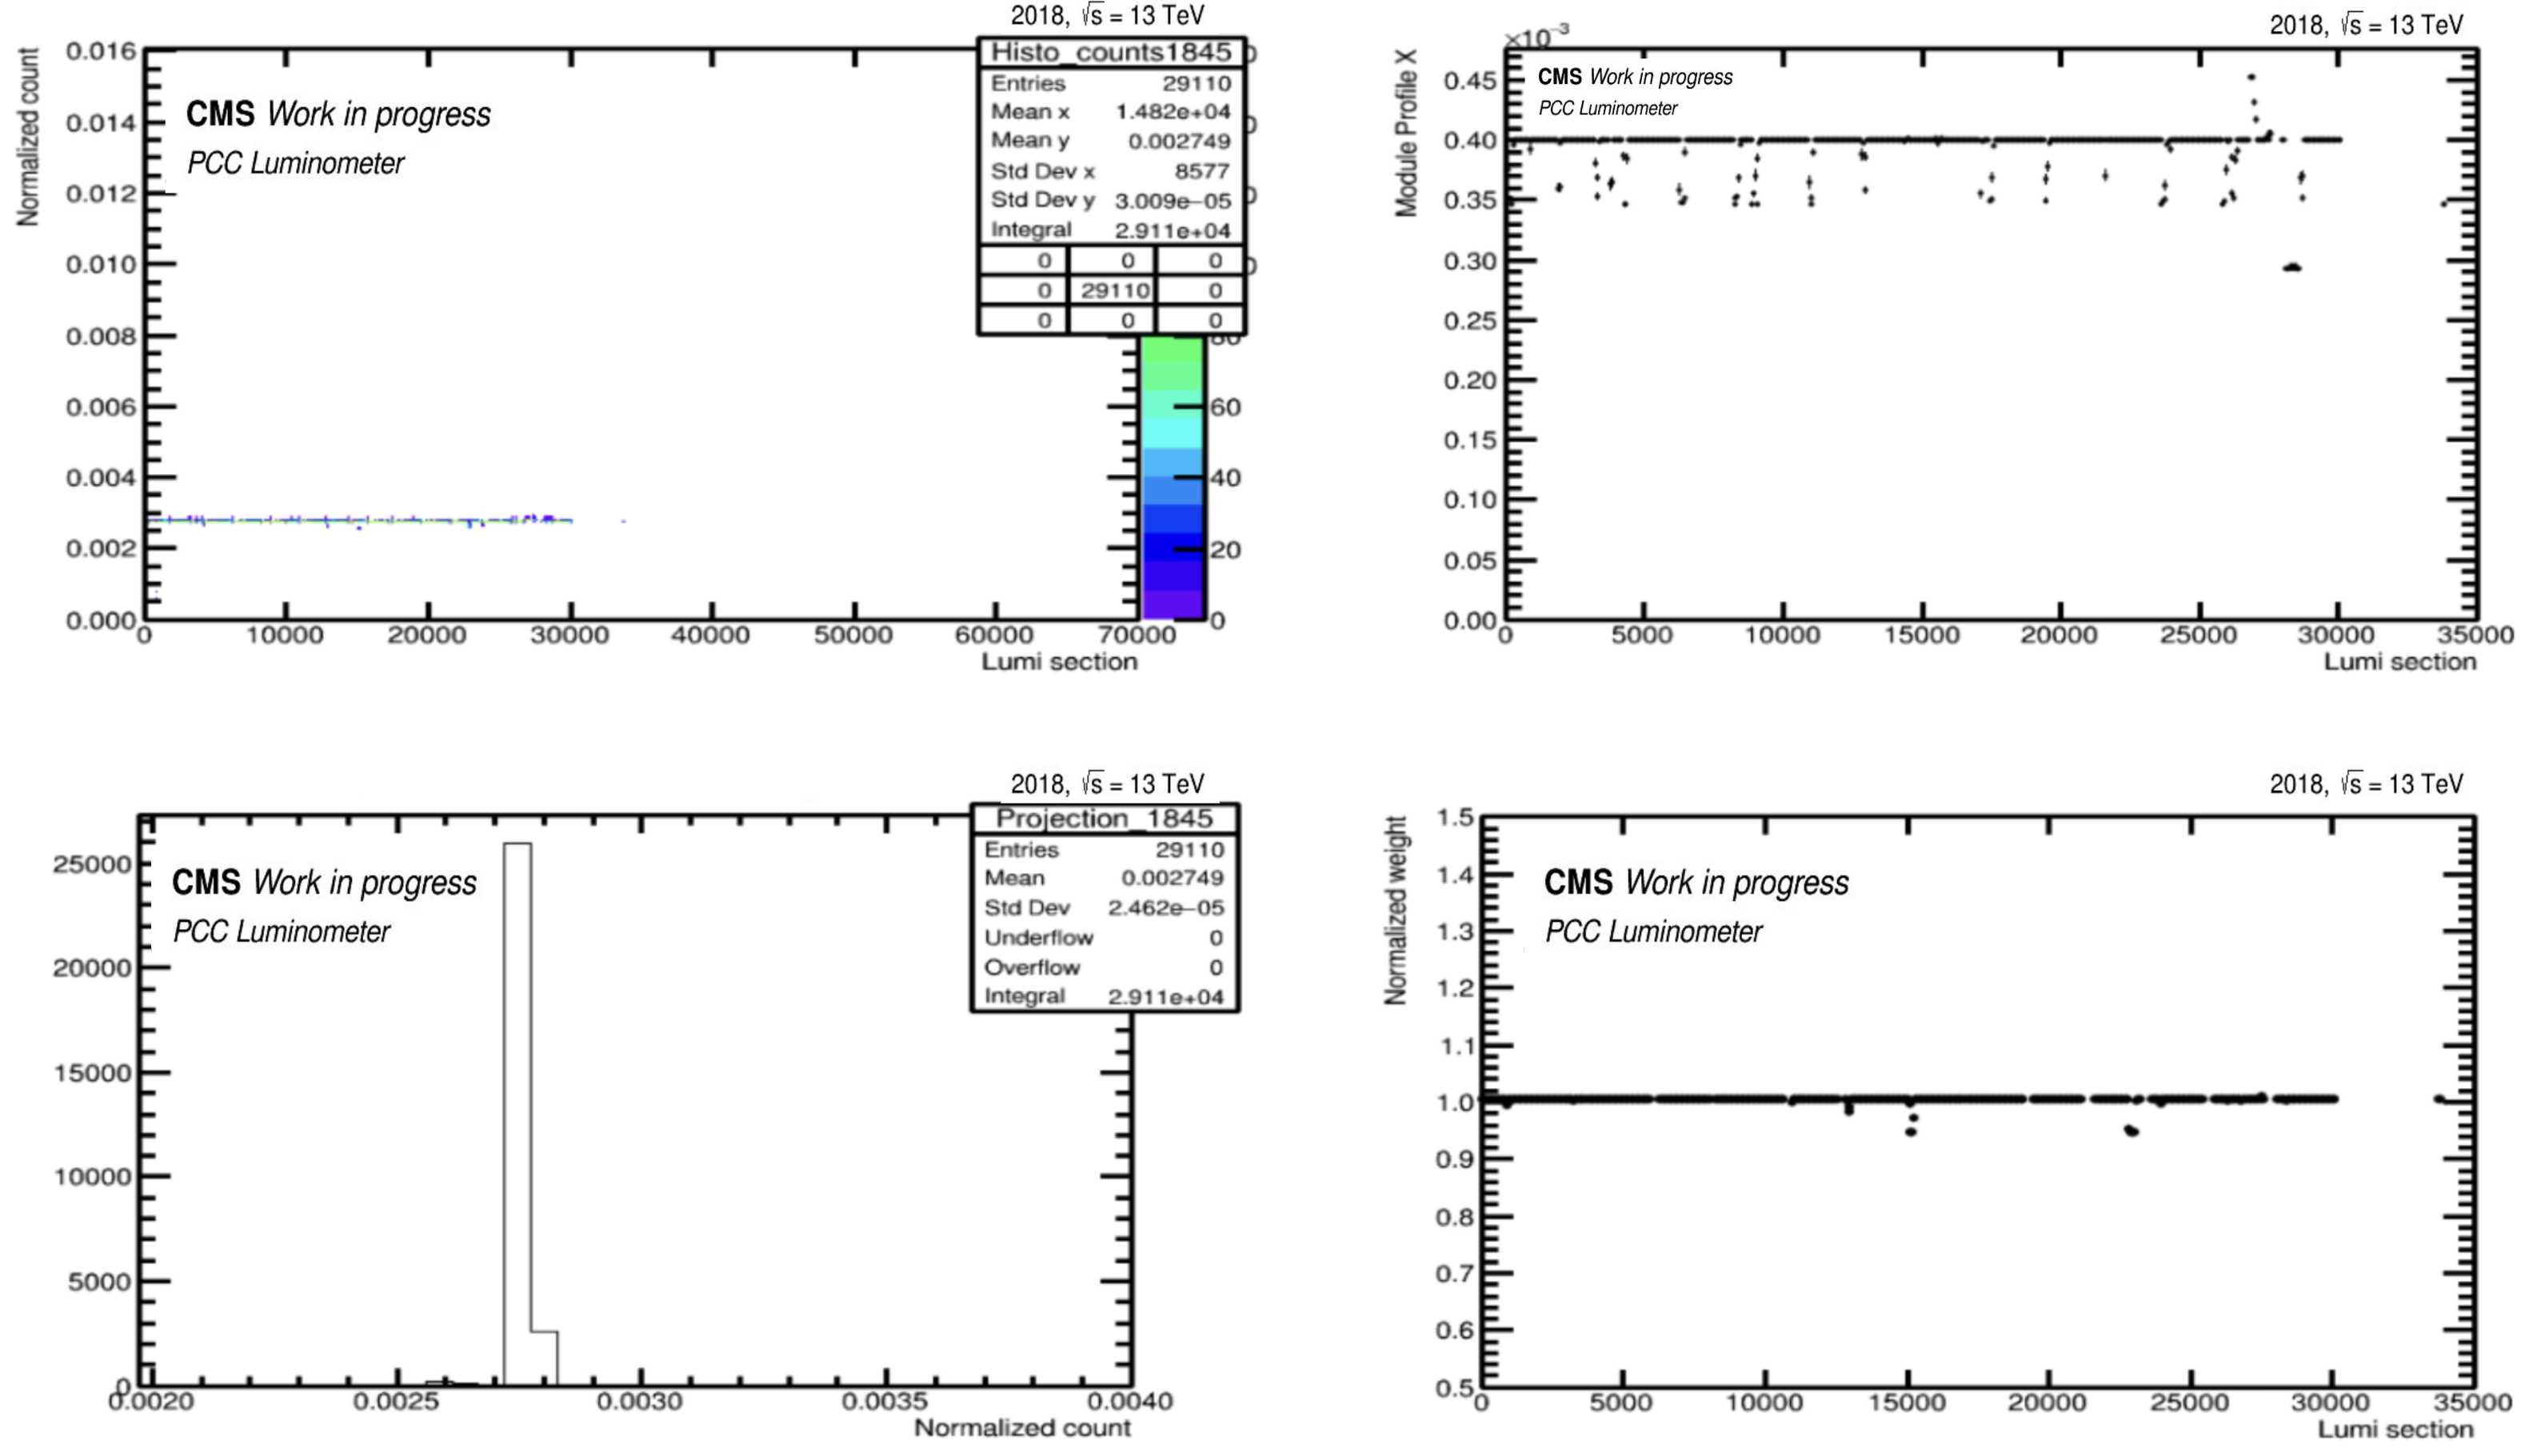
\includegraphics[width=1\textwidth]{ashish_thesis/Module_weight_2.png}
%\caption[Module Weight]{%
 %  Method to obtain module weights as a function of lumi section for categorizing good and bad modules. X profile of TH2F histogram (module PCC/total PCC per lumi section) is obtained. X profile is then filled in a TGraph after removing points with error $>$ 0.05. TGraph is normalized with the mean of Y projection of TH2F histogram to obtain module stability profile.
%}
%\label{fig:mod_weight}
%\end{figure}


\begin{figure}[!htp]
\centering
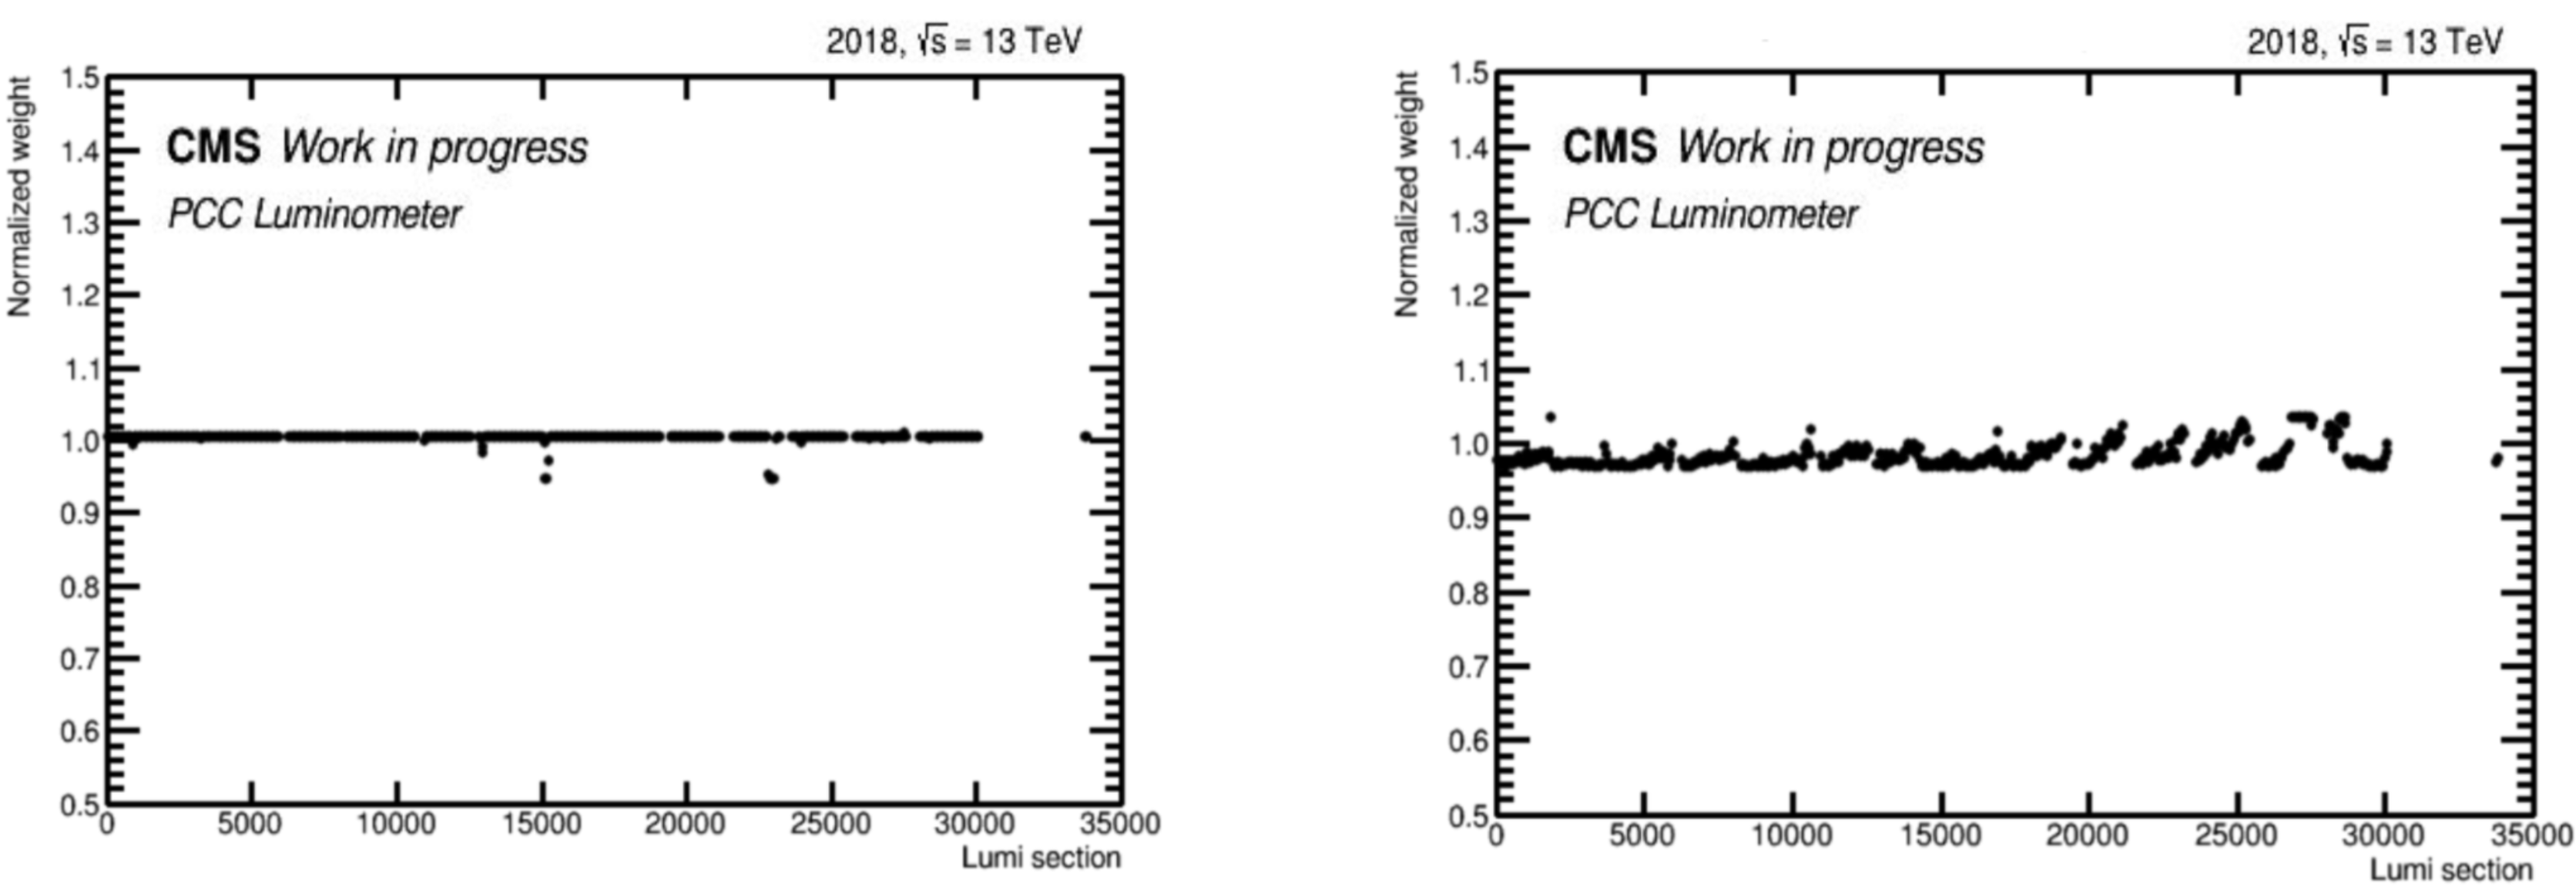
\includegraphics[width=1\textwidth]{ashish_thesis/good_bad_modules_1.png}
\caption[Good/Bad Module Weights]{%
   Change in normalized module weight with time. Modules showing significant change in module weight (shown in right figure) over time having large RMS/mean values are used to make module veto list.
}
\label{fig:goodbadmodules}
\end{figure}

The module veto list is a list of detector modules that are excluded from the analysis of data due to their known or suspected high rate of background events or other issues that could affect the accuracy of the measurement. The following factors lead to unstable modules: 

\begin{itemize}

\item Radiation damage: The harsh radiation environment in the LHC can cause damage to the silicon pixel sensors over time, leading to increased leakage currents, noise, or reduced charge collection efficiency.

\item Manufacturing defects: Defects in the silicon material or issues during the manufacturing process can result in poorly performing pixel modules. These defects may not be immediately evident but can become more pronounced overtime.

\item Electronic noise: Noisy electronic components or crosstalk between channels can lead to an increased number of false signals or noise in the pixel module data.

\item Temperature variations: Temperature fluctuations can affect the performance of the pixel modules, leading to changes in their noise levels, gain, or charge collection efficiency.

\item High voltage issues: Problems with the high voltage supply to the pixel modules can result in unstable operation, leading to erratic behavior or complete module failure.

\item Partial module failure: A pixel module may suffer from partial failure, with some pixels or readout channels not functioning properly. This can lead to an increased number of dead or noisy pixels in the module.

\item Readout or data acquisition issues: Errors in the readout electronics or data acquisition system can lead to data corruption or loss, affecting the performance of the pixel modules.

\item Calibration issues: Inaccurate or outdated calibration parameters can result in incorrect measurements, leading to the appearance of abnormal behavior in the pixel module data.

\item Firmware or software issues: Bugs in the firmware or software responsible for controlling and reading out the pixel modules can lead to abnormal behavior or incorrect measurements.

\item Mechanical or alignment issues: Mechanical stresses or misalignments during the installation or operation of the pixel detector can affect the performance of the pixel modules or cause them to fail.

\item Contamination or environmental factors: Contamination of the pixel modules by dust, moisture, or other substances can affect their performance or cause them to fail. Similarly, external environmental factors, such as magnetic fields or vibrations, can impact the operation of the pixel modules.

\end{itemize}

%The inclusion of certain modules in the veto list is based on a careful analysis of the detector performance and the expected background rates in a given experiment. By excluding modules with high background rates or other issues, the analysis can be improved and the accuracy of the measurement can be increased.

Module veto list consisting of bad modules is first created for period B, vdM Fill and then for other periods A, C, D1, D2, D3 and D4 as follows, 

Run 2018B and vdM Fill:
\begin{itemize}

\item Poor statistics lumi sections are removed by applying selection on total PCC. %Fig. \ref{fig:PCC_cut}. % and \ref{fig:f_it}.

\item All barrel layer 1 modules are removed as these modules are significantly affected by dynamic inefficiency effects, where the hit efficiency decreases at higher instantaneous luminosity due to the readout chip not being able to process all of the hits.
  
\item A loose selection of 7\% based on RMS/mean of module weight profile is applied where mean and RMS values are obtained from y projection of module weight profile. Modules with significantly large RMS/mean are removed with this loose selection as shown in Fig. \ref{fig:outliermodules}. 

\item Module stability is re-evaluated based on RMS/mean values using an iterative method where in each step, appropriate selections are applied to remove bad modules (shown in Fig. \ref{fig:sec_it_cut}) until stable luminosity is attained.                                                      
\end{itemize}

Run 2018A, C and D:                                                                      
\begin{itemize}  

\item Period B module vetolist is applied to these periods to determine remaining bad modules.

\item same procedure is used as period B. 

\item module weight comparisons between period B and these periods is done and modules with more than 3 sigma change in module weights are removed as shown in %Fig. \ref{fig:mod_w_com} and
  Fig \ref{fig:mod_w_com_1}.                                                                              
\end{itemize}

%\begin{figure}[t]
%\centering
%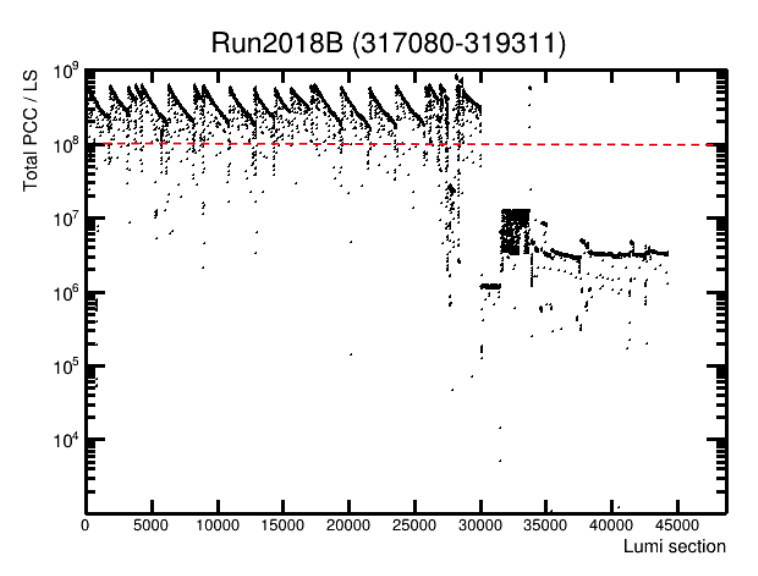
\includegraphics[width=0.7\textwidth]{ashish_thesis/Run2018B_totalPCC_cut.png}
%\caption[Low Statistics Lumi section Filtering]{%
% Total PCC as a function of lumi section for period 2018B. Appropriate selection on total PCC shown by the red line is applied to remove low statistics lumi sections.
%}
%\label{fig:PCC_cut}
%\end{figure}

%\begin{figure}[!htp]
%\centering
%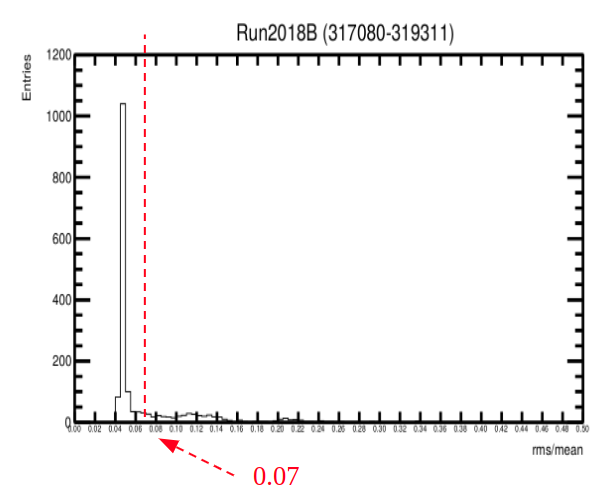
\includegraphics[width=0.7\textwidth]{ashish_thesis/first_iteration.png}
%\caption{%
%   A loose cut of 7\% is applied on rms/mean values of module stability profile to remove outlier modules.
%}
%\label{fig:f_it}
%\end{figure}

\begin{figure}[!htp]
\centering
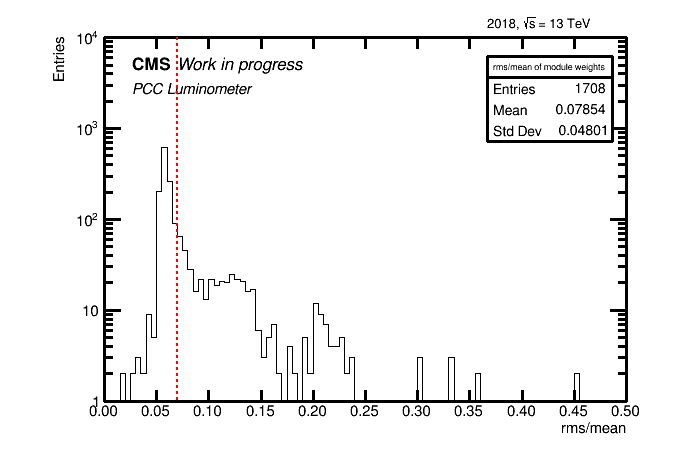
\includegraphics[width=0.8\textwidth]{ashish_thesis/cut_selection_1.png}
\caption[First Iteration For Outlier Module Removal]{%
   A loose selection of 7\% is applied to remove bad modules. Appropriate selections are applied in each iterative step to remove other bad modules.
}
\label{fig:outliermodules}
\end{figure}

\begin{figure}[!htp]
    \centering
    %\begin{minipage}{0.45\textwidth}
        \centering
        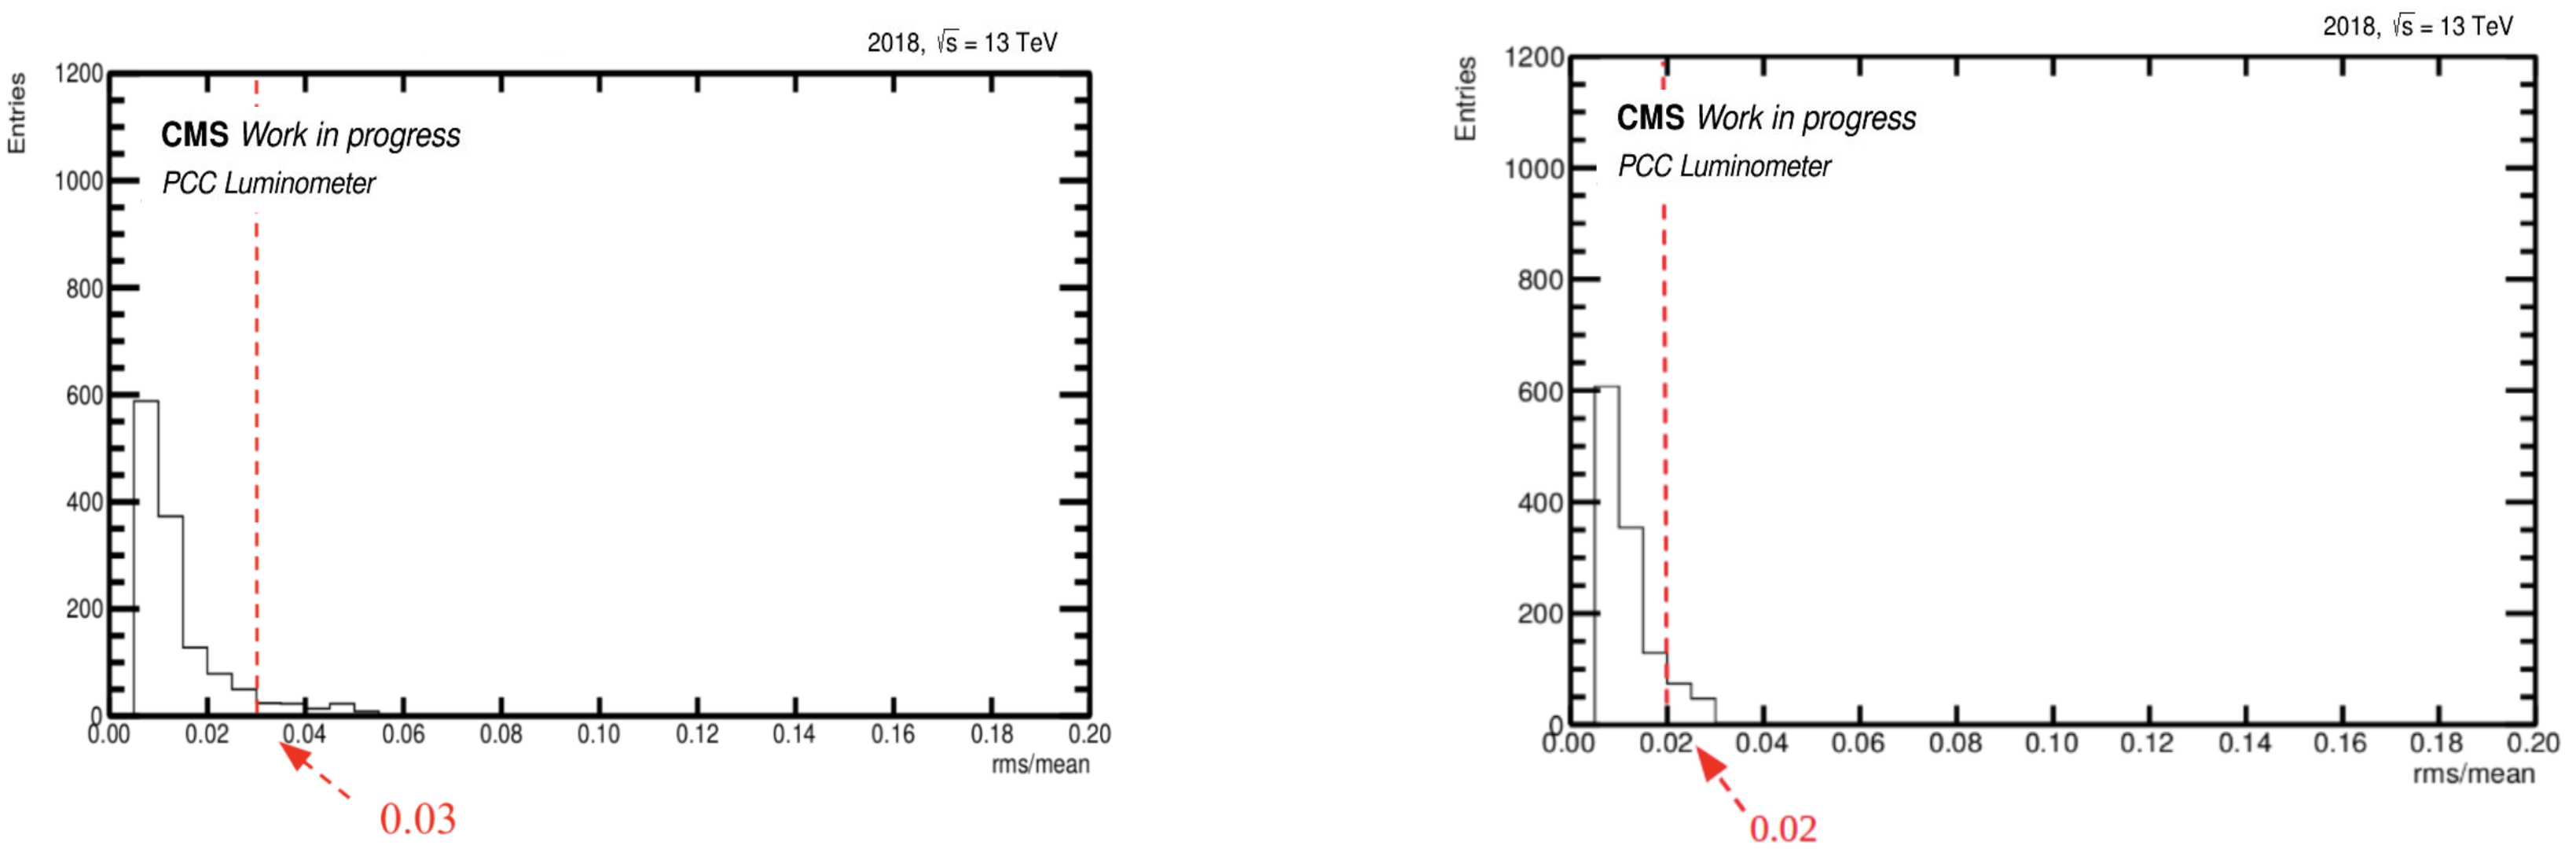
\includegraphics[width=1.0\linewidth]{ashish_thesis/3percent_cut_1.png}
    %\end{minipage}
    %\hfill
    %\begin{minipage}{0.45\textwidth}
     %   \centering
      %  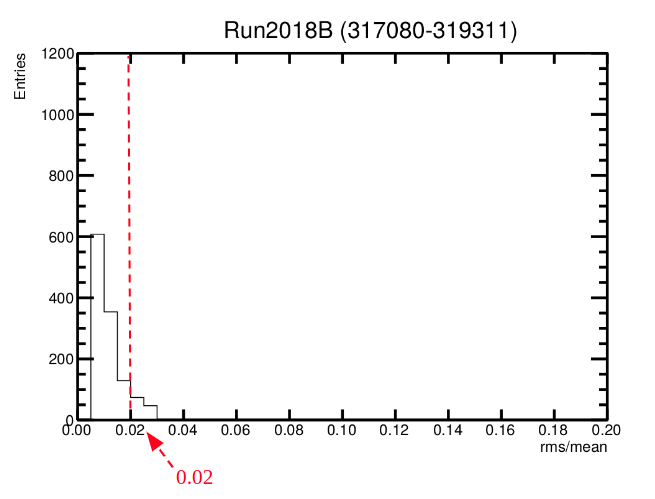
\includegraphics[width=1.0\linewidth]{ashish_thesis/second_iteration_cut.png}
    %\end{minipage}
    
    \caption[Second and Final Iteration For Outlier Module Removal]{%
        Left: Second iteration on RMS/mean of 3\% is applied to remove more bad modules. 
        Right: Final iteration on RMS/mean of 2\% is applied to obtain module veto list for each period.
    }
    \label{fig:sec_it_cut}
\end{figure}








\begin{comment}

\begin{figure}[!htp]
\centering
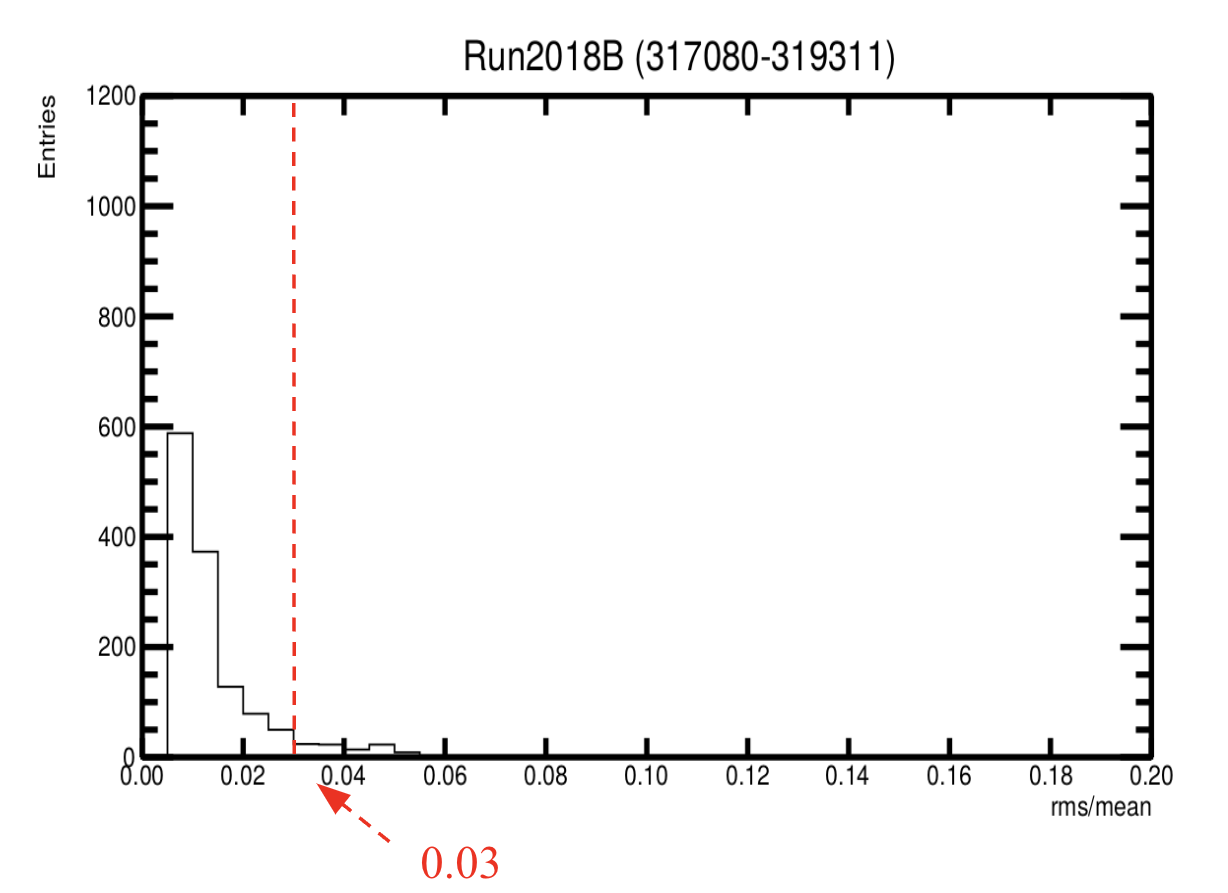
\includegraphics[width=0.6\textwidth]{ashish_thesis/3percent_cut.png}
\caption[Second Iteration For Outlier Module Removal]{%                                                                                                                                                                                       
 Second selection on RMS/mean of 3\% is applied to obtain module veto list for each period.
}
\label{fig:second_it_cut}
\end{figure}


\begin{figure}[!htp]
\centering
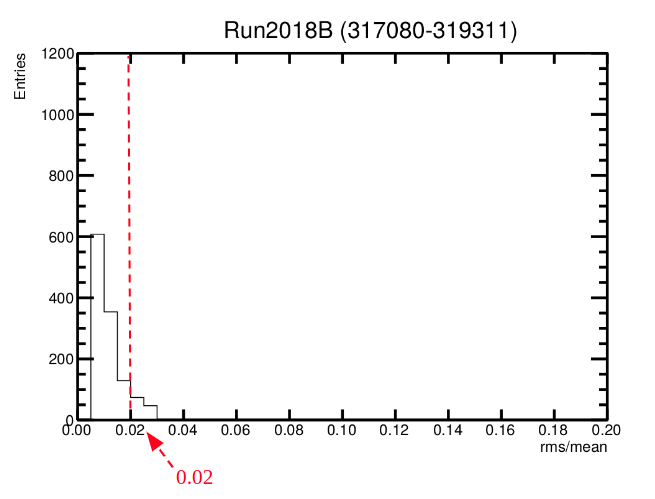
\includegraphics[width=0.6\textwidth]{ashish_thesis/second_iteration_cut.png}
\caption[Final Iteration For Outlier Module Removal]{%
 Final selection on RMS/mean of 2\% is applied to obtain module veto list for each period.
}
\label{fig:sec_it_cut}
\end{figure}

\end{comment}

%\begin{figure}[!htp]
%\centering
%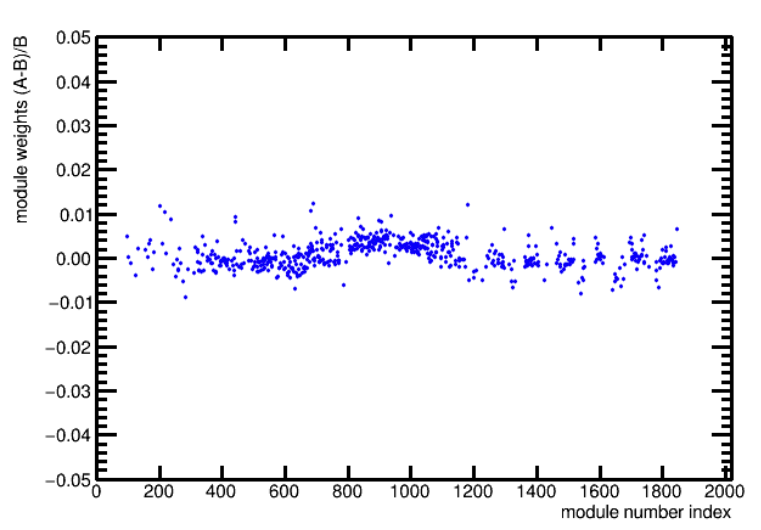
\includegraphics[width=1\textwidth]{ashish_thesis/mod_weight_comparison.png}
%\caption{%
%   Change in module weights between period A and B for all modules left after applying 2\% rms module vetolist.
%}
%\label{fig:mod_w_com}
%\end{figure}


\begin{figure}[!htp]
\centering
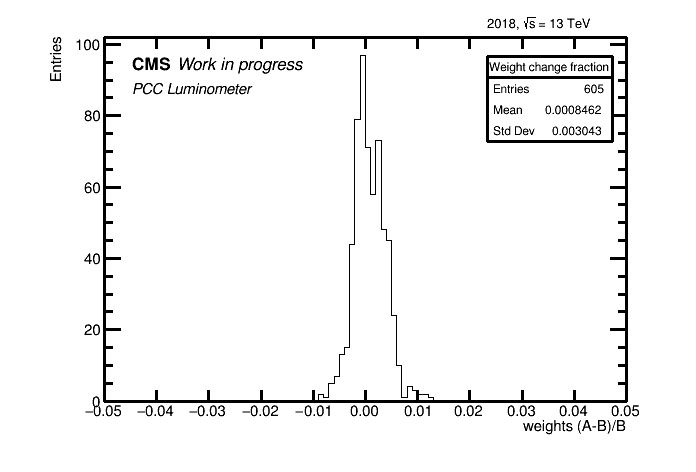
\includegraphics[width=0.7\textwidth]{ashish_thesis/mod_weight_comp_2.png}
\caption[Module Weights Change Removal]{%
   Projection of change in module weights between period A and B. Modules showing more than 3 sigma change in module weights are added to the module veto list.
}
\label{fig:mod_w_com_1}
\end{figure}
   
 2\% selection on RMS/mean of module weights gives the best stability for all pixel detector barrel layers and forward disks. Number of good and bad modules after this selection is shown in Table \ref{tab:per period veto}. % Bad modules found after applying this 2\% selection in the final iterative step are used to constitute a 2 $\%$ rms module veto list for each period as shown in Table \ref{tab:per period veto}. 
                                                                                 
 \begin{table}
   \begin{center}
     \caption[Good/bad modules for each period]{2 \% rms module veto list for each period showing number of good and bad modules.}
    \begin{tabular}{ccccc}  
    \textbf{Period}   & \textbf{\# bad modules} & \textbf{\# good modules} \\ \hline
     A      &   1276   &  580    \\  
     B      &    802  &     1054  \\ 
     C      &   1076  &    780   \\ 
     D1     &  1169  &     687  \\ 
     D2     &  1184  &    672   \\ 
     D3     &  1081  &    775   \\ 
     D4     &  1032  &     824  \\ 
      \end{tabular}
    %\caption[Good and bad modules during each period]{2 \% rms module veto list for each period showing number of good and bad modules.}
    \label{tab:per period veto}
  \end{center}
\end{table}


\begin{comment}

Table \ref{tab:pccvis_diffveto} depicts the mean and RMS values of PCC/HFOC luminosity for each period using per period veto list. The mean values are demonstrated for periods A, B, C, D1, D2, D3, and D4, with 'A' having a mean value of 1.006 and the other periods ranging from 0.9981 to 1.003. The RMS values range from 0.002115 to 0.004183, showing a degree of variation. The table also provides the ratio of RMS to mean, which offers a perspective on relative fluctuations. The calculated ratios are close to their corresponding RMS values, indicating relatively consistent variability across periods. The table effectively illustrates a nuanced variation in mean luminosity values across different periods.

\begin{table}[!ht]
\centering
%\topcaption{%
 %PCC/ HFOC luminosity mean and rms values for new per period vetolist showing variation in mean values across period.
%}
\begin{tabular}{ccccc}
    \textbf{Period} & \textbf{mean} & \textbf{rms} &  \textbf{rms/mean} \\ \hline
    A & 1.006 & 0.004183 & 0.004158 \\
    B & 0.9981  & 0.003133 & 0.0031389 \\
    C & 0.9989  & 0.003009 & 0.003012\\
    D1 & 1.003  & 0.002441 & 0.002433 \\
    D2 & 1.001  & 0.0029 & 0.00289 \\
   D3  & 1  & 0.002115 & 0.002115 \\
   D4  & 1.002  & 0.003673 & 0.003666 \\ 
\end{tabular}
\caption[Mean value change for PCC/HFOC across period.]{%                                                                                                                                       
 PCC/ HFOC luminosity mean and rms values for  per period veto list showing variation in mean values across period.
}
\label{tab:pccvis_diffveto}
\end{table}


\end{comment}

Figure \ref{fig:b_a_stability_vdm} shows the stability plots of the relative contribution to luminosity from pixel layers/disks before and after applying the module veto in the vdM calibration period. %This veto list application is essential for maintaining data quality as it helps to filter out data from modules showing more than 2\% variability in their RMS/mean, considered potentially large.
The plots provide a comparative view of how the luminosity fraction has been impacted by the application of this veto list. The 'before' plot shows greater variability, reflecting the fluctuations in luminosity across different layers or disks  during each lumi section. In contrast, the 'after' plot  display a more stable profile, indicating that the module selection has effectively reduced the variance in luminosity fraction readings, enhancing data stability. %This figure plays a crucial role in visualizing the impact of implementing stringent data vetting procedures in the analysis of luminosity measurement.
%An improvement in the stability of various PCC layer and disk for the whole Period B after applying new veto list shown in Fig. \ref{fig:old_new_periodB}.

\begin{figure}[!htp]
\centering
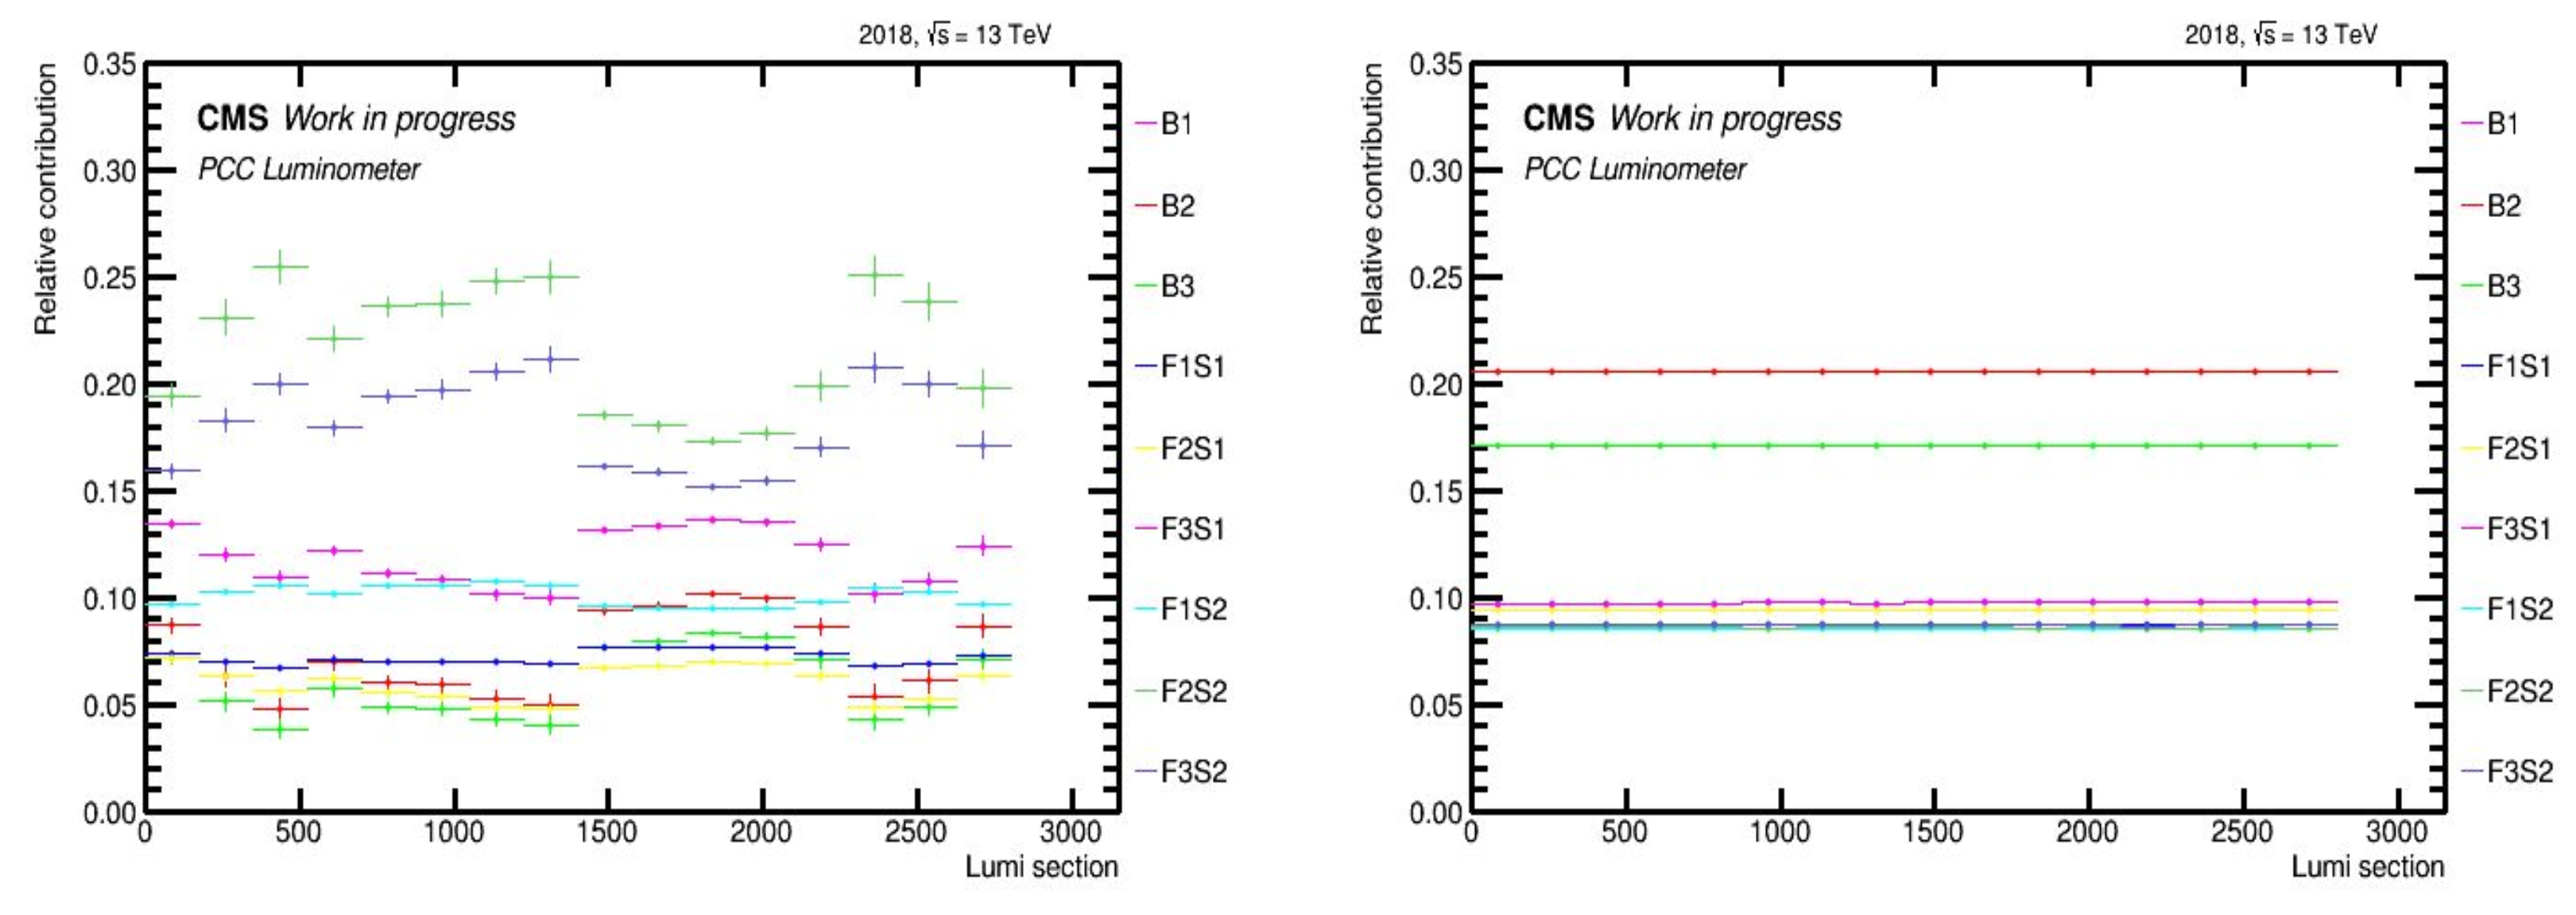
\includegraphics[width=1\textwidth]{ashish_thesis/before_after_vdm_stability_1.png}
\caption[PCC vdM Stability]{%                                                                                                                                                                      
   Luminosity fraction per layer or disk (stability plots) before (no veto) and after applying the final module veto with 2\% RMS/mean selection for the vdM fill data.
}
\label{fig:b_a_stability_vdm}
\end{figure}

%\begin{figure}[!htp]
%\centering
%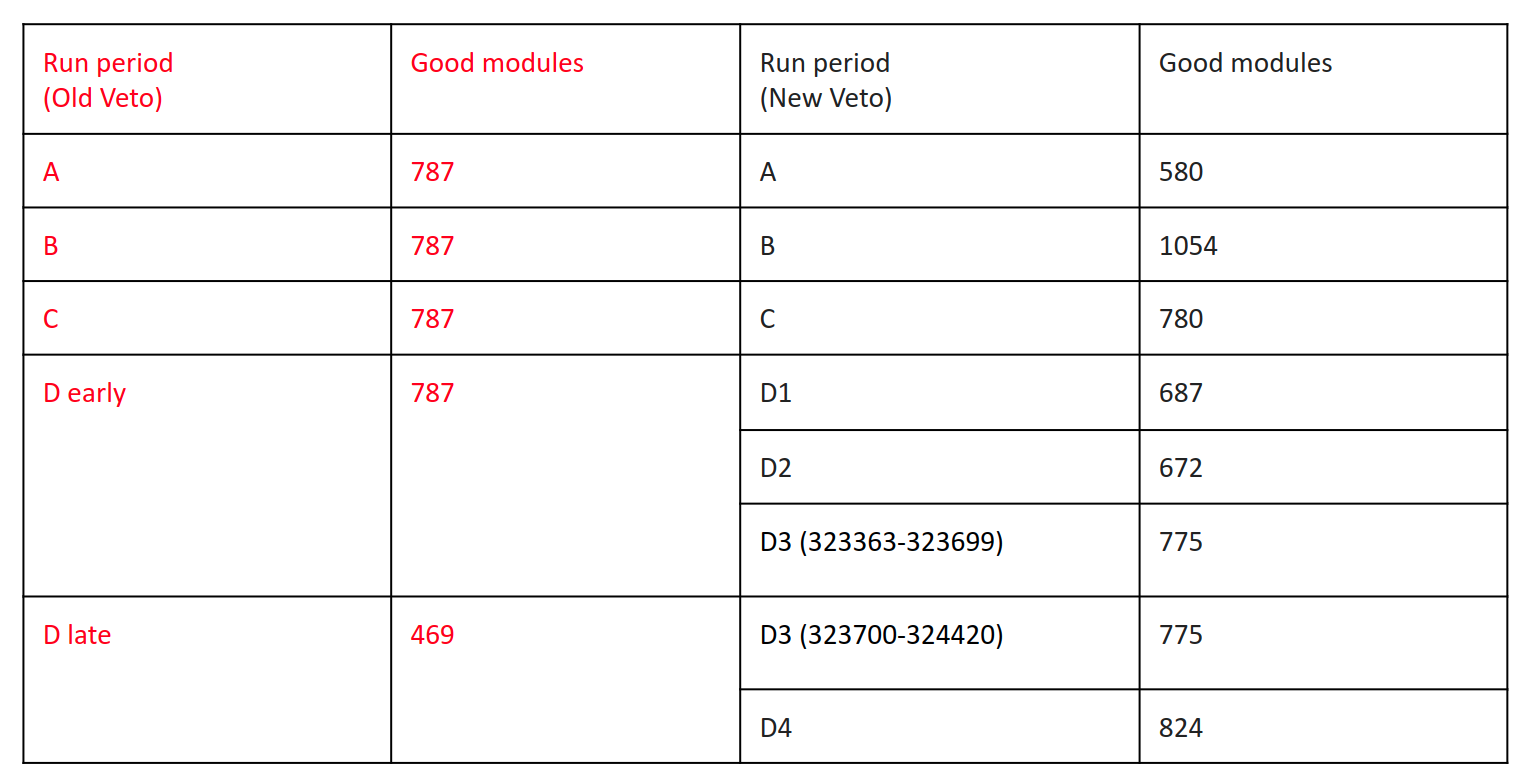
\includegraphics[width=0.8\textwidth]{ashish_thesis/old_new_veto.png}
%\caption{%
 %  klm
%}
%\label{fig:old_new_vetolist}
%\end{figure}

\begin{comment}
  
Table \ref{tab:runperiod_oldnew} details the number of "Good Modules" across different run periods under both old and new veto conditions. The periods under consideration are A, B, C, and D, with D further subdivided into "early" and "late" phases for the old veto. In the new veto, period D is segmented into D1, D2, D3 (split into two specific run ranges), and D4. Under the "Old Veto" condition, periods A, B, C, and "D early" each have a consistent count of 787 good modules. However, for the "D late" phase, there are 469 good modules, suggesting a notable reduction from the earlier phase of period D. Moving to the "New Veto" scenario, the good modules count shows considerable variability across periods. Period A records 580 good modules, B has the highest number with 1054, and C presents 780 good modules. For the D period under the new veto, D1 and D2 show 687 and 672 good modules respectively. Period D3, divided into two separate run ranges (323363-323699 and 323700-324420), maintains a consistent count of 775 good modules for both ranges. Finally, for period D4, there are 824 good modules.

\begin{table}
  \centering
  \caption{Run Period and Good Modules}
\begin{tabular}{cccc}
\textbf{Run period (Old Veto)} & \textbf{Good modules} & \textbf{Run period (New Veto)} & \textbf{Good modules} \\
\hline
A & 787 & A & 580 \\
B & 787 & B & 1054 \\
C & 787 & C & 780 \\
D early & 787 & D1 & 687 \\
 & & D2 & 672 \\
 &  & D3 (323363-323699)  &  775\\
D late & 469 & D3 (323700-324420) & 775 \\
&  & D4 & 824\\
\end{tabular}
%\caption{Run Period and Good Modules}
\label{tab:runperiod_oldnew}
\end{table}

\end{comment}

%An improvement in the stability of various PCC layer and disk is shown in Fig. \ref{fig:old_new_periodB} after applying new veto list.

%\begin{figure}[!htp]
%\centering
%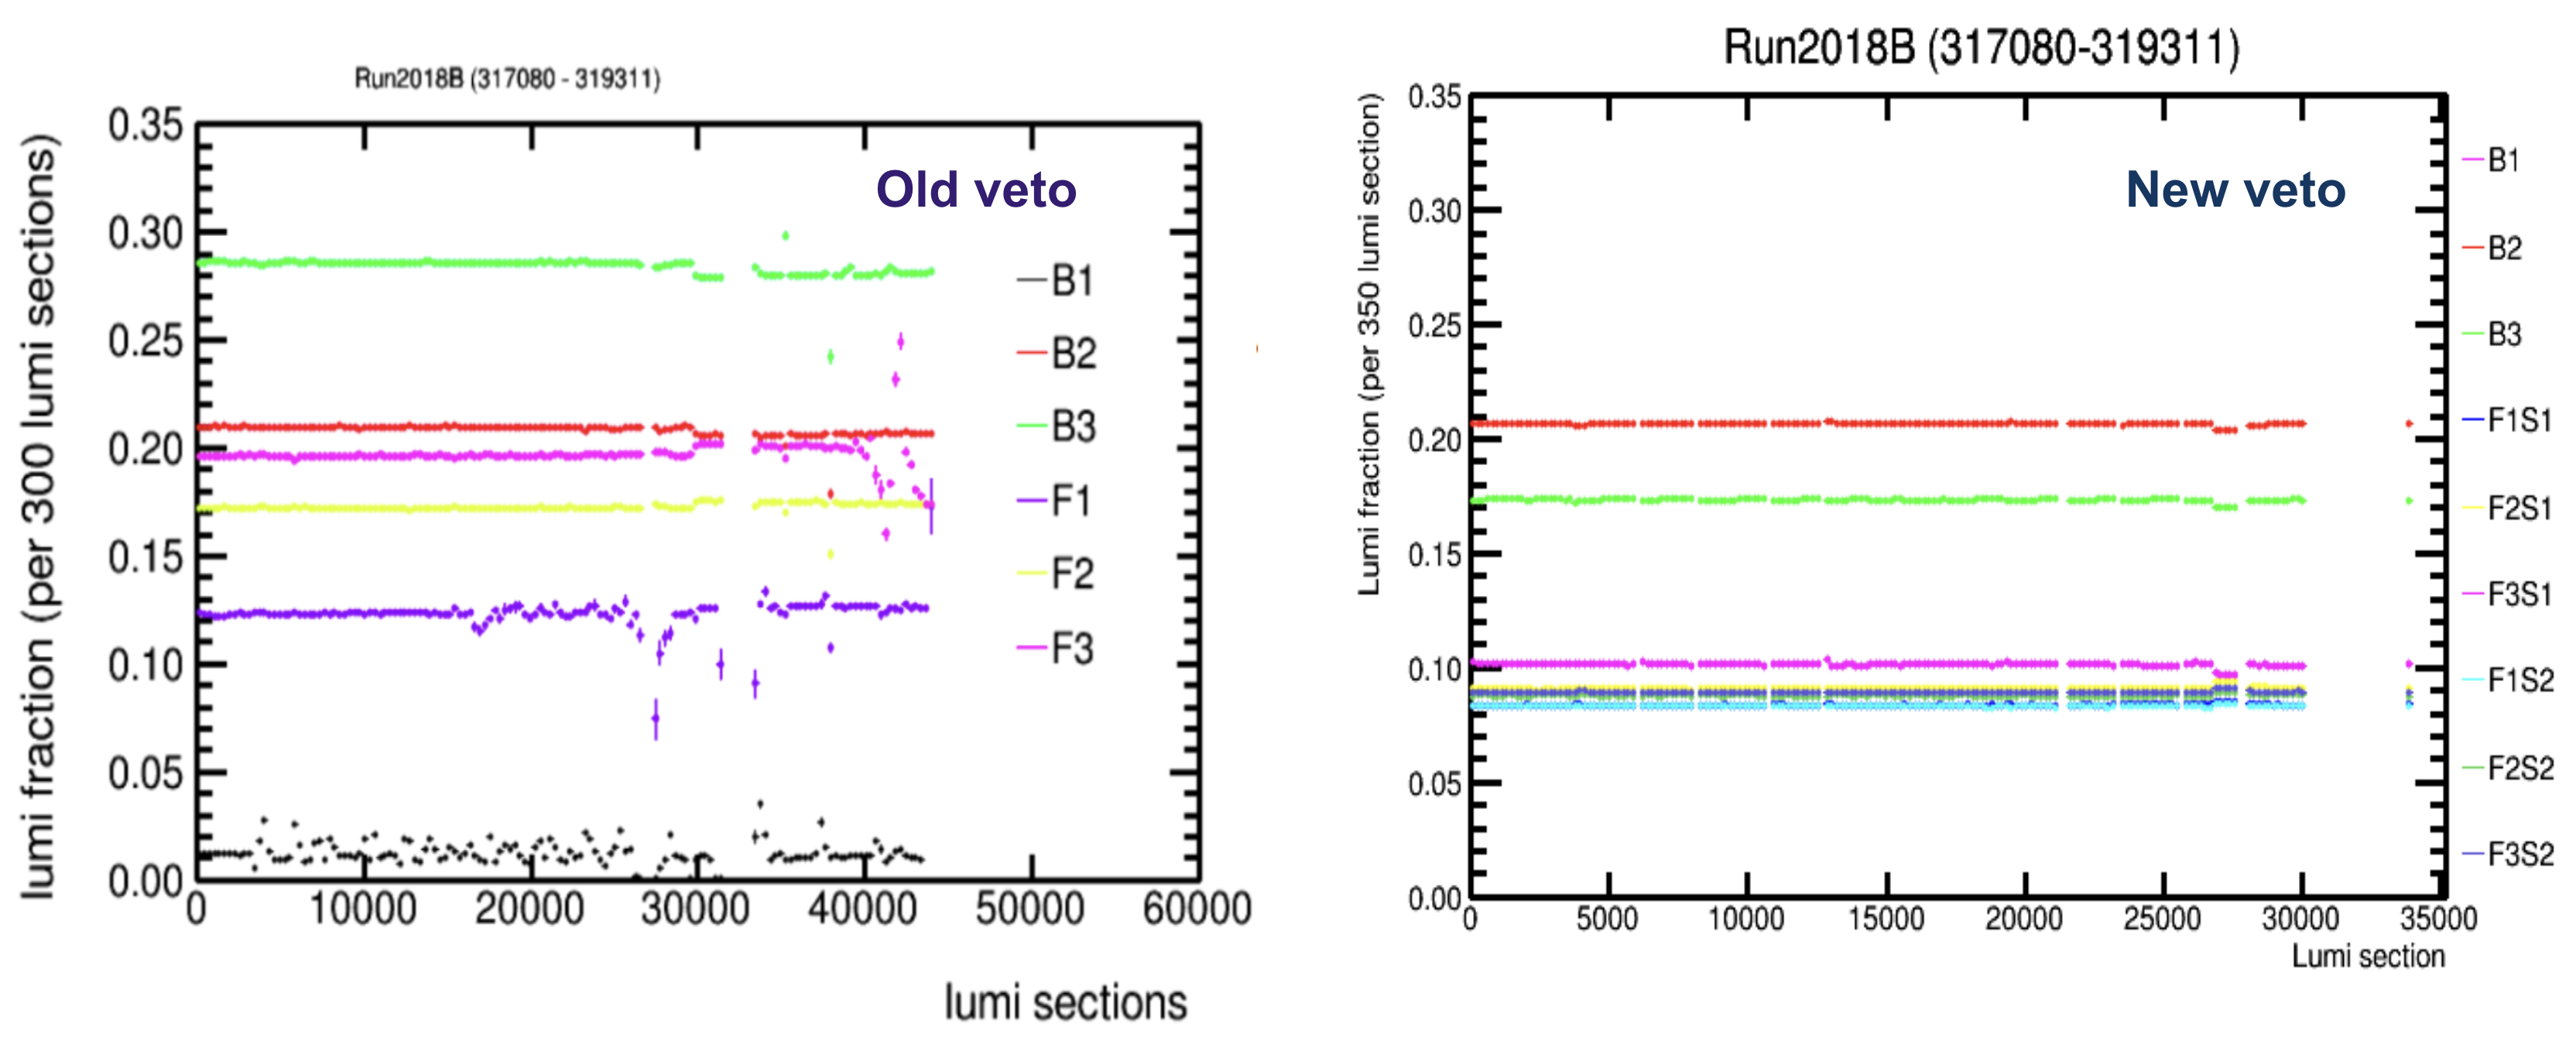
\includegraphics[width=1\textwidth]{ashish_thesis/old_new_veto_periodB.png}
%\caption[Old new veto period B per layer/disk stability]{Comparison of PCC layer and disk stability for old and new module veto.}
%\label{fig:old_new_periodB}
%\end{figure}

%To reduce the variation in mean values across periods thereby improving the stability of PCC luminometer, a common module veto list is created using the 2\% RMS/mean selection as shown in Table \ref{tab:2commonveto}.

Table \ref{tab:2commonveto} shows the number of modules for a common selection over the entire year. Common module veto list is a combination of module veto list of all run periods A, B, C, D1, D2, D3 and D4. Approach to make a common module veto list is to start by combining module vetolists of period A,B and C, then combine A,B, C, D1 and so on. Less than $9\%$ of the pixel modules remain after applying module stability selections to be used for final luminosity measurement. The total number of good modules across all layers and disks is 155.


\begin{table}
  \begin{center}
    \caption[Common module veto list]{Final module veto list. This veto list is created by combining module veto lists for each period.}
    \begin{tabular}{ccccc}  
      \textbf{Period}   & \textbf{\# bad modules} & \textbf{\# good modules} \\  \hline
      A + B  & 1276 & 580 \\
     A + B + C      &  1417   &  439    \\  
     A + B + C + D1      &   1534  &   322    \\ 
     A + B + C + D1 + D2      &   1629 &    227   \\ 
     A + B + C + D1 + D2 + D3     &   1668 &   188    \\ 
     A + B + C + D1 + D2 + D3 + D4     &  1701 &     155  \\ 
      \end{tabular}
    %\caption[Common module veto list for all periods]{Final module veto list. This veto list is created by combining module veto lists for each period.}
    \label{tab:2commonveto}
  \end{center}
\end{table}

%\begin{figure}[!htp]
%\centering
%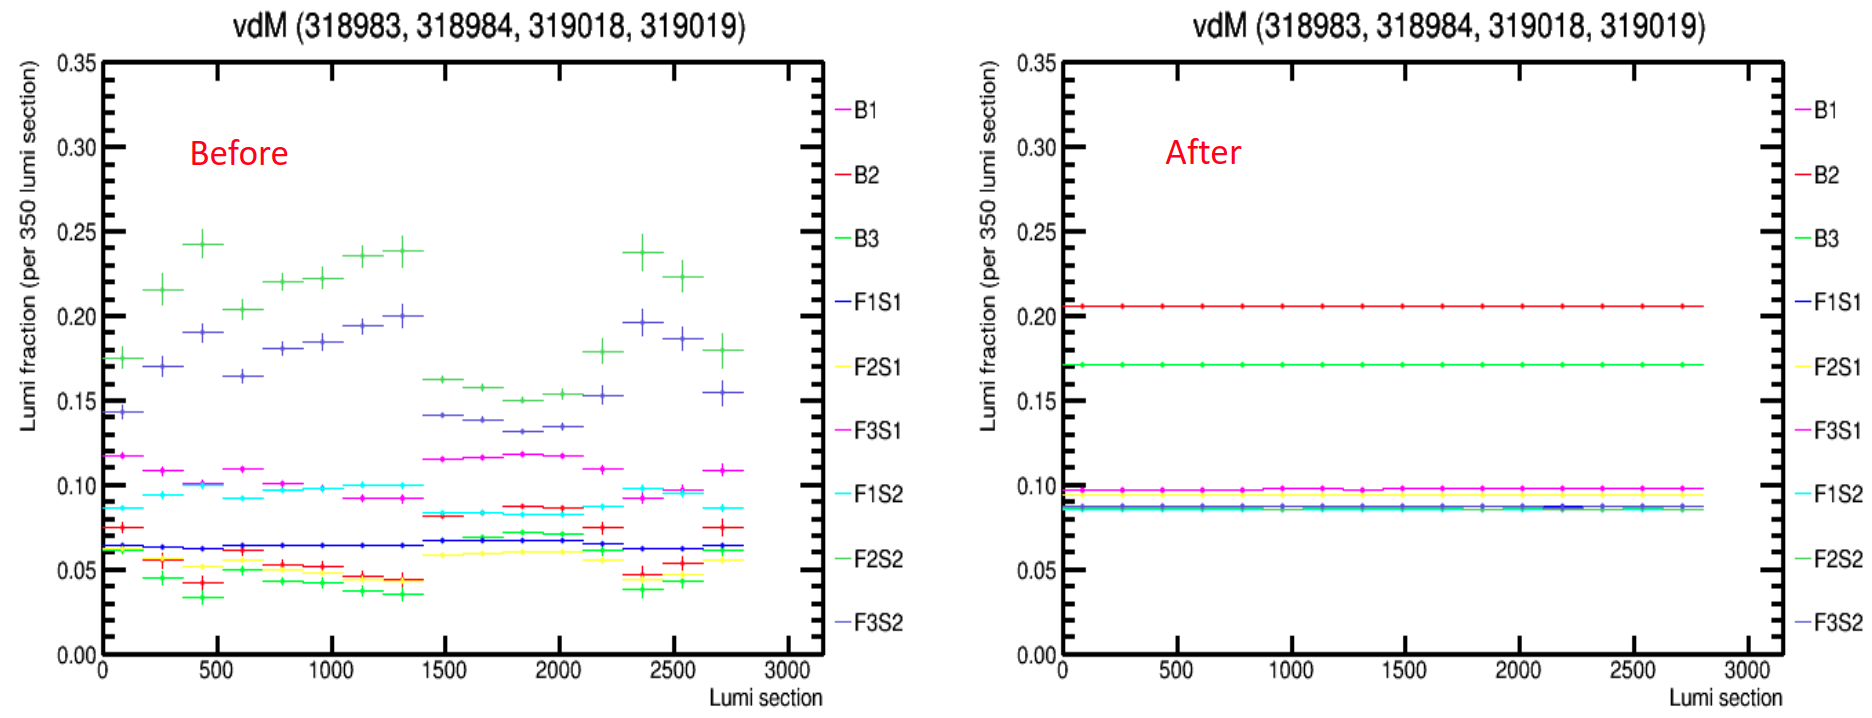
\includegraphics[width=1\textwidth]{ashish_thesis/before_after_vdm_stability.png}
%\caption[]{%
 %  Luminosity fraction (stability plots) before and after applying 2\% rms module vetolist.
%}
%\label{fig:b_a_stability_vdm}
%\end{figure}

%\begin{figure}[!htp]
%\centering
%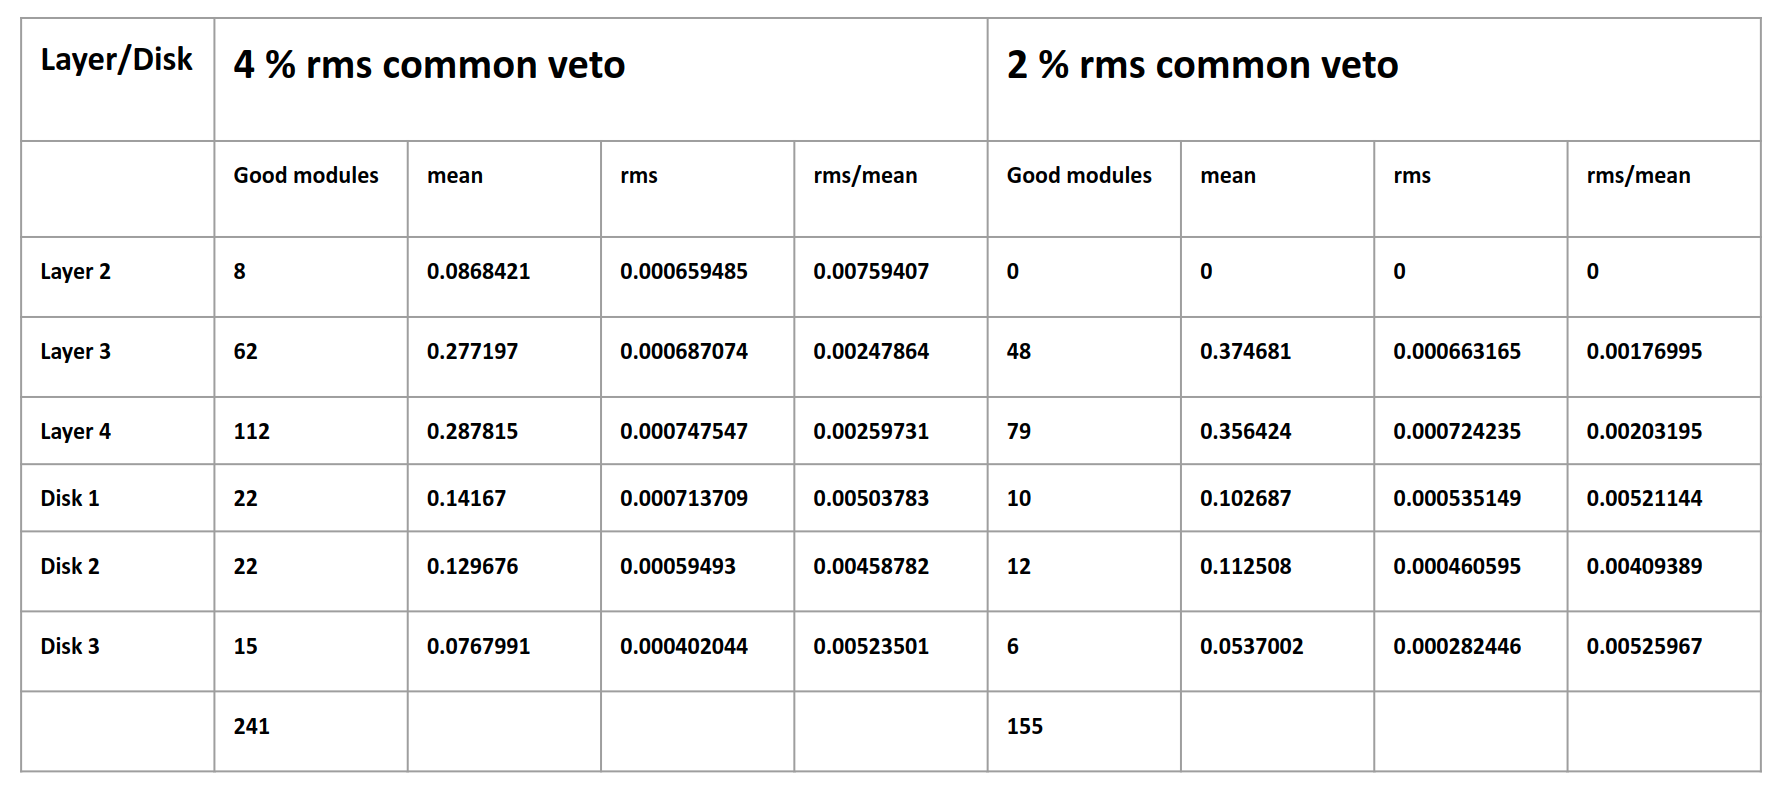
\includegraphics[width=1\textwidth]{ashish_thesis/pcc_layer_disk_mean_rms.png}
%\caption{%
%pcc layer disk mean rms
%}
%\label{fig:pixellalyerdiskmeanrms}
%\end{figure}

%\begin{table}[htbp]
%\centering
%\caption{Layer/Disk Statistics}
%\label{tab:layer-disk}
%\begin{tabular}{cccccc}
%\textbf{Layer/Disk} & \textbf{Good modules} & \textbf{mean} & \textbf{rms} & \textbf{rms/mean} \\
%\hline
%Layer 2 & 0 & 0 & 0 & 0 \\
%Layer 3 & 48 & 0.374681 & 0.000663165 & 0.00176995 \\
%Layer 4 & 79 & 0.356424 & 0.000724235 & 0.00203195 \\
%Disk 1 & 10 & 0.102687 & 0.000535149 & 0.00521144 \\
%Disk 2 & 12 & 0.112508 & 0.000460595 & 0.00409389 \\
%Disk 3 & 6 & 0.0537002 & 0.000282446 & 0.00525967 \\
%Total  & 155 & & \\
%\multicolumn{2}{c}{} & \multicolumn{2}{r}{155} \\
%\end{tabular}
%\caption{Layer/Disk Statistics}
%\end{table}

The relative contribution to PCC luminosity from each pixel detector layer and disk without and with final module veto list is shown in Fig. \ref{fig:stabprof_4333}.

%\begin{figure}[!htp]
%\centering
%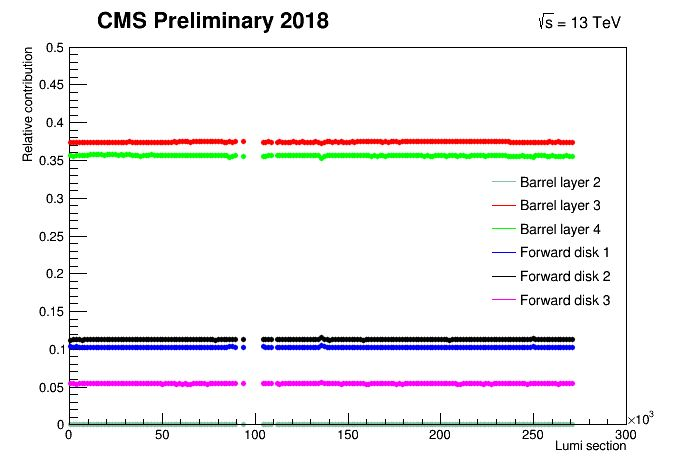
\includegraphics[width=0.8\textwidth]{ashish_thesis/2percentcommonveto_pixellayerdisk.png}
%\caption[Pixel layer/disk stability]{%
 %  Stability profiles of pixel detector layer and disk modules for 2\% rms common module veto list.
%}
%\label{fig:stabprof}
%\end{figure}

\begin{figure}[!htp]
\centering
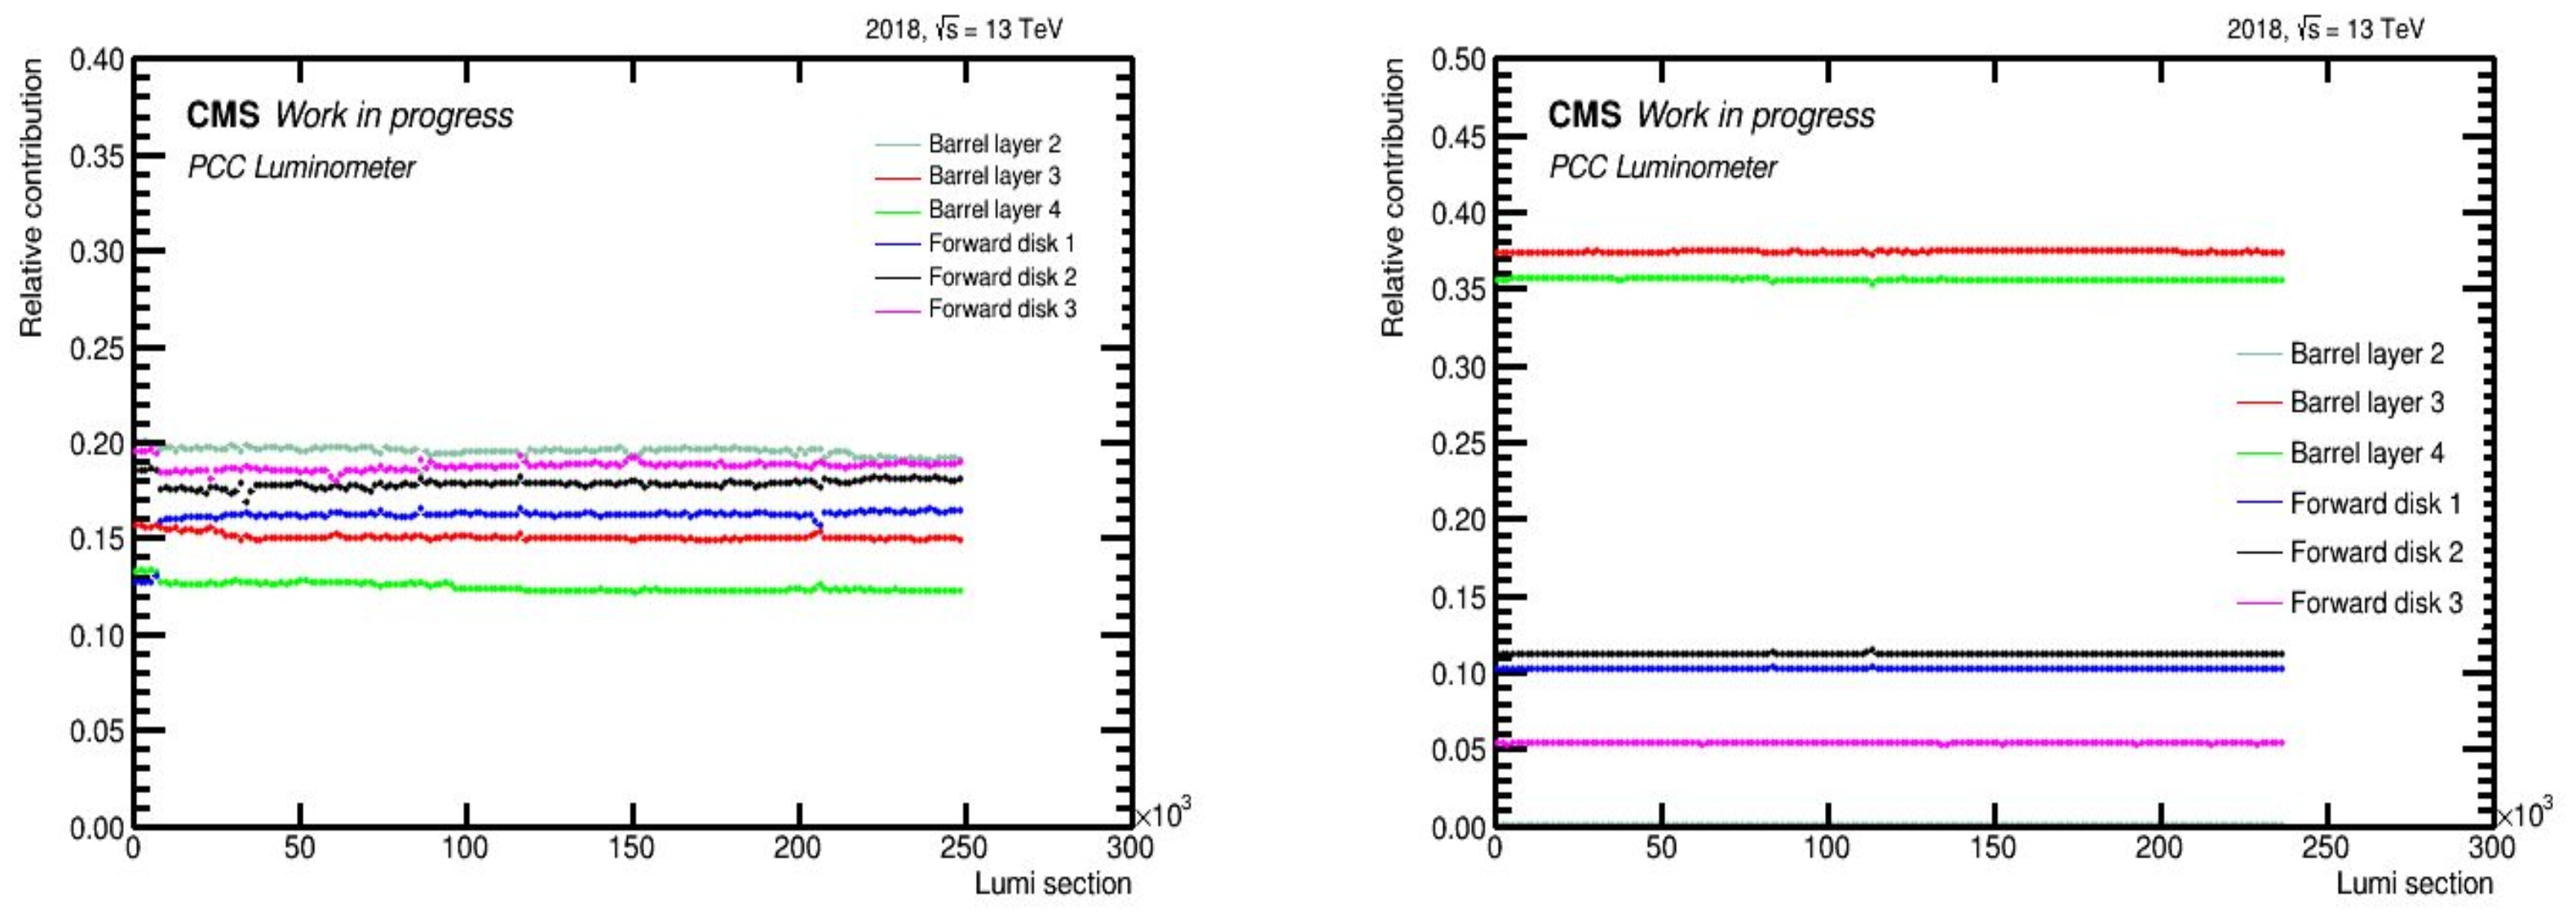
\includegraphics[width=\textwidth]{ashish_thesis/2percentcommonveto_pixellayerdisk_1.png}
\caption[PCC Stability For Physics Runs]{Left: Luminosity fraction of pixel detector for various layer and disks as a function of lumi section for a module selection excluding only the BPIX Layer 0 for the full 2018 zero-bias dataset. Right: Stability profiles of pixel detector layer and disk for final module veto list.}
\label{fig:stabprof_4333}
\end{figure}

%\begin{figure}[!htp]
 % \centering
  %\begin{subfigure}[b]{0.49\textwidth}
   % 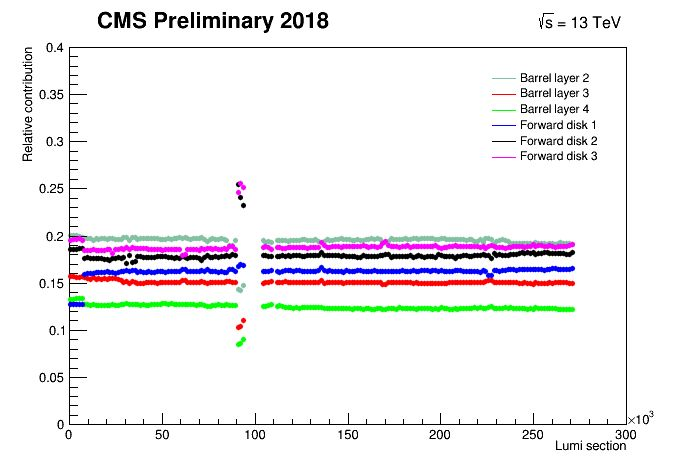
\includegraphics[width=\textwidth]{ashish_thesis/pixel_layer_disk_B0_veto.png}
    %\caption{Image 1}
  %\end{subfigure}
  %\hfill % or \hspace{5mm} for a specific horizontal space
  %\begin{subfigure}[b]{0.49\textwidth}
   % 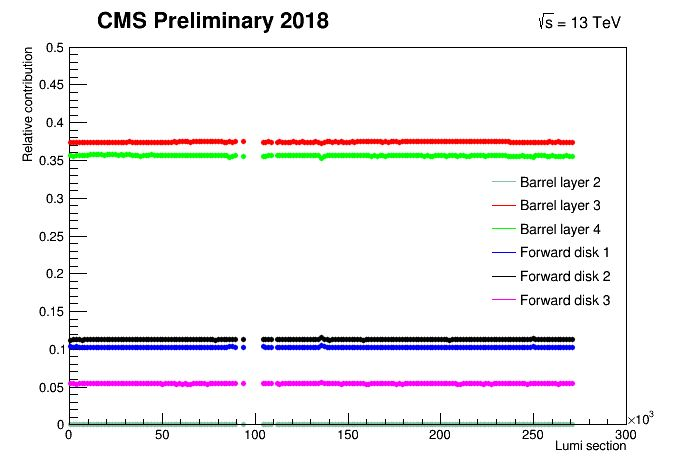
\includegraphics[width=\textwidth]{ashish_thesis/2percentcommonveto_pixellayerdisk.png}
    %\caption{Image 2}
  %\end{subfigure}
  %%\caption[PCC Stability For Physics Runs]{Left: Luminosity fraction of pixel detector for various layer and disks as a function of lumi section for a module selection excluding only the BPIX Layer 0 for the full 2018 zero-bias dataset. Right: Stability profiles of pixel detector layer and disk for final module veto list.}
  %\label{fig:stabprof_4333}
%\end{figure}

Table \ref{tab:layer-disk} presents the statistics of good modules across different layers and disks for final module veto list. The layers and disks are divided into five categories: Layer 3, Layer 4, Disk 1, Disk 2, and Disk 3. For each of these categories, the number of good modules, mean, RMS, and the ratio of RMS to mean are provided. Layer 2 has no good modules. %and all statistical parameters are zero.
Layer 3, on the other hand, has 48 good modules with a mean value of 0.374681, an RMS of 0.000663165 and an RMS-to-mean ratio of 0.00176995, indicating low variability. Layer 4 shows a slightly larger count of good modules with 79, and similar statistical parameters to Layer 3, albeit with a slightly higher RMS and RMS-to-mean ratio, suggesting slightly greater variability. When it comes to the disk categories, Disk 1 and Disk 2 each have 10 and 12 good modules respectively. Their mean values are lower than those of the layers, as are their RMS values, although their RMS-to-mean ratios are higher, suggesting greater relative variability in these categories. Disk 3 has the fewest good modules with only 6, and it presents the highest RMS-to-mean ratio among all categories, indicating the highest relative variability. %The total number of good modules across all layers and disks is 155.
%It's noteworthy that the table does not provide an aggregated mean, RMS, or RMS-to-mean ratio across all categories.

\begin{table}[!htp]
  \centering
  \caption[Final module veto statistics]{Layer/Disk good modules and statistics for final module veto list.}
%\caption{Layer/Disk Statistics}                                                                                                                                                                       
%\label{tab:layer-disk}
\begin{tabular}{cccccc}
\textbf{Layer/Disk} & \textbf{Good modules} & \textbf{mean} & \textbf{rms} & \textbf{rms/mean} (\%) \\
\hline
Layer 3 & 48 & 0.374681 & 0.000663165 & 0.176995 \\
Layer 4 & 79 & 0.356424 & 0.000724235 & 0.203195 \\
Disk 1 & 10 & 0.102687 & 0.000535149 & 0.521144 \\
Disk 2 & 12 & 0.112508 & 0.000460595 & 0.409389 \\
Disk 3 & 6 & 0.0537002 & 0.000282446 & 0.525967 \\
Total  & 155 & & \\
%\multicolumn{2}{c}{} & \multicolumn{2}{r}{155} \\                                                                                                                            
\end{tabular}
%\caption[Final veto statistics]{Layer/Disk good modules and statistics for final module veto list.}
\label{tab:layer-disk}
\end{table}

\section{vdM calibration results}

The calibration of luminosity measurement by the CMS experiment luminometers in the 2018 proton-proton data taking at $\sqrt{s}$ = 13 TeV \cite{pas_18} was performed during LHC fill 6868 on June 30 and July 1, 2018 at $\sqrt{s}$ = 13 TeV. Zero-bias triggers on 5 bunch pairs (BCIDs 265, 865, 1780, 2192, and 3380) recorded events rate is 27.7 kHz. Trigger is applied on five colliding bunches due to limitation of the recording bandwidth.

%\item "lsc1", was the "constant separation" scan, two beams were separated by 1.4 $\sigma$ and moved together in steps of 1 $\sigma$ across and back. %\item "lsc2", was the "variable separation" scan method, one beam (starting with beam 1) is moved to -2.5 $\sigma$ and then a three-point scan (a "miniscan") is performed with the other beam.                         %a normal VdM scan pair "norm4" and two short emittance scan pairs "emit4" and "emit5" were also performed.     %The 2018 CMS VdM scan program was conducted in two segments, interrupted by an alarm. The first segment involved six x-y scan pairs. Two were short ``emittance'' scans, named ``emit1'' and ``emit2,'' where the beamswere separated by $ \(4\sigma_b\) $ over 9 steps with a 10 second integration time at each step. A standard VdM scan, named ``norm1,'' separated the beams by $\(6\sigma_b \approx 600\)~\mu m$ in 25 steps, with a 30-second duration per step. The ``offset1'' scan followed the same procedure as the standard scans but with a $\(\pm 1.5\sigma_b\)$ separation in the non-scanning direction. Lastly, two sets of ``beam imaging'' scans wereconducted, where one beam remained fixed while the other was moved in 19 steps between $\(+4.5\sigma_b\)$ and $\(-4.5\sigma_b\)$, each lasting 46 seconds per step.                                                      
The 2018 CMS vdM scan program (shown in Fig. \ref{fig:vdm_prog_2018}) was conducted in two segments, interrupted by an alarm. The first segment involved six x-y scan pairs. Two were short ``emittance'' scans, named ``emit1'' and ``emit2,'' where the beams were separated by \(4\sigma_b\) over 9 steps with a 10-second integration time at each step. A standard vdM scan (described in section 3.1), named ``vdM1,'' separated the beams by \(6\sigma_b \approx 600\)~$\mu$m in 25 steps, with a 30-second duration per step. The ``offset1'' scan followed the same procedure as the standard scans but with a \(\pm 1.5\sigma_b\) separation in the non-scanningdirection. Lastly, two sets of ``beam imaging'' scans were conducted, where one beam remained fixed while the other was moved in 19 steps between \(+4.5\sigma_b\) and \(-4.5\sigma_b\), each lasting 46 seconds per step. The second part of the scan program was conducted in the same fill, approximately 7.5 hours later, and consisted of twelve scan pairs. This included a short emittance scan, ``emit3''; beam imaging scan pairs, ``imag2'' and``imag3''; an offset scan pair, ``offset2''; and two standard vdM scan pairs, ``vdM2'' and ``vdM3''.

Beam Imaging Scans: Beam imaging scans are designed to measure the transverse profile of the beam. They involve moving one beam across the other in steps and measuring the interaction rate (or event rate) at each step. By doing this, the shape or "profile" of the beam in the transverse plane can be obtained. These scans allow for a detailed analysis of the beam shape, which is essential for understanding the beam properties. In a perfect scenario, the density distributions of protons in a bunch would factorize into separate X (horizontal) and Y (vertical) components. However, real beams can have correlations between X and Y (non-factorization). Beam imaging scans help map the 2D profile of the beam and are thus essential for diagnosing and understanding any such correlations. Knowing the 2D profile of the beams is crucial when calculating luminosity, as assumptions made about the factorization of the beam profiles feed into these calculations. By using beam imaging scans, experimenters can assess the validity of the factorization assumption or correct for any observed non-factorization.

Offset Scans: %Offset scans are performed to check for systematic errors in the luminosity measurement, which may arise from various sources.
They are similar to standard VdM scans but involve an intentional offset in the non-scanning direction. By comparing the results of offset scans with the results of regular scans, one can identify and correct for any systematic discrepancies that are present. Offset scans can help to assess the sensitivity of the luminosity measurement to non-factorization in the transverse plane. For example, if there are correlations between the X and Y distributions of protons (i.e., non-factorization), this could in principle affect the shape of the beam overlap region in the collision point. Offset scans, by changing the relative position of the beams, can help to assess whether such non-factorization has a significant effect on the measured luminosity.

vdM scans are typically conducted at least once a year to ensure the luminometer is correctly calibrated. Results of these scans that is the visible cross section is used to normalize the data collected by the experiments during physics run.

\begin{figure}[!htp]
    \centering
    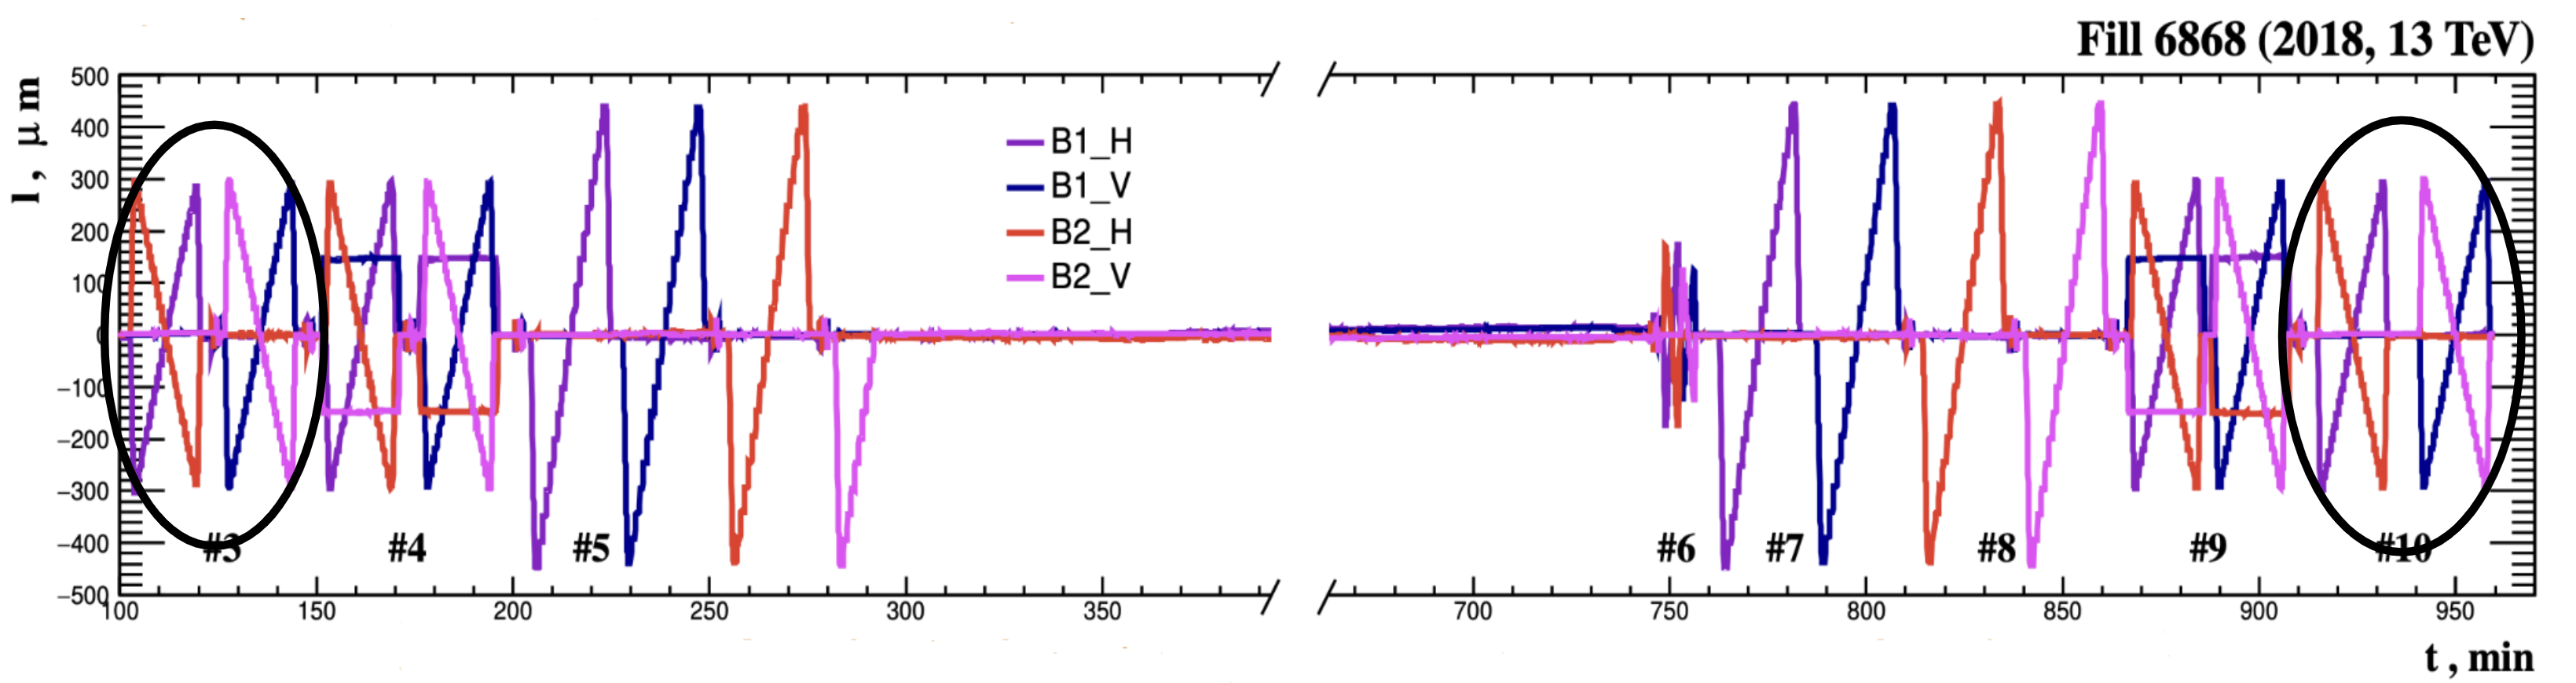
\includegraphics[width=1\textwidth]{ashish_thesis/vdm_program_2018.png}
    \caption[2018 vdM Program]{Beam position along x and y is plotted as a function of time showing different types of scans. #3 and #10 are vdM scans, #4 and #9 are offset scans, #5, #7 and #8 are beam imaging scans, #6 is emittance scan.}
    \label{fig:vdm_prog_2018}
\end{figure}

The vdM data (LHC fill 6868) is processed using the final module selection. The background estimation for the PCC rate is done with two super-separation scans SS1 and SS2. The mean and error are obtained from the $y$ projection of PCC per NB4 plotted as a function of time as shown in Fig. \ref{fig:sigmavis_ss_backg}. The results for five different BCIDs are shown in Table \ref{tab:vdm:SS1_SS2}, using the reprocessed PCC data for Fill 6868. The overall background correction applied to raw PCC rate is $0.02757\pm0.01987$, which is calculated by taking the average of the mean values of SS1 and SS2.


\begin{figure}[!htp]
\centering
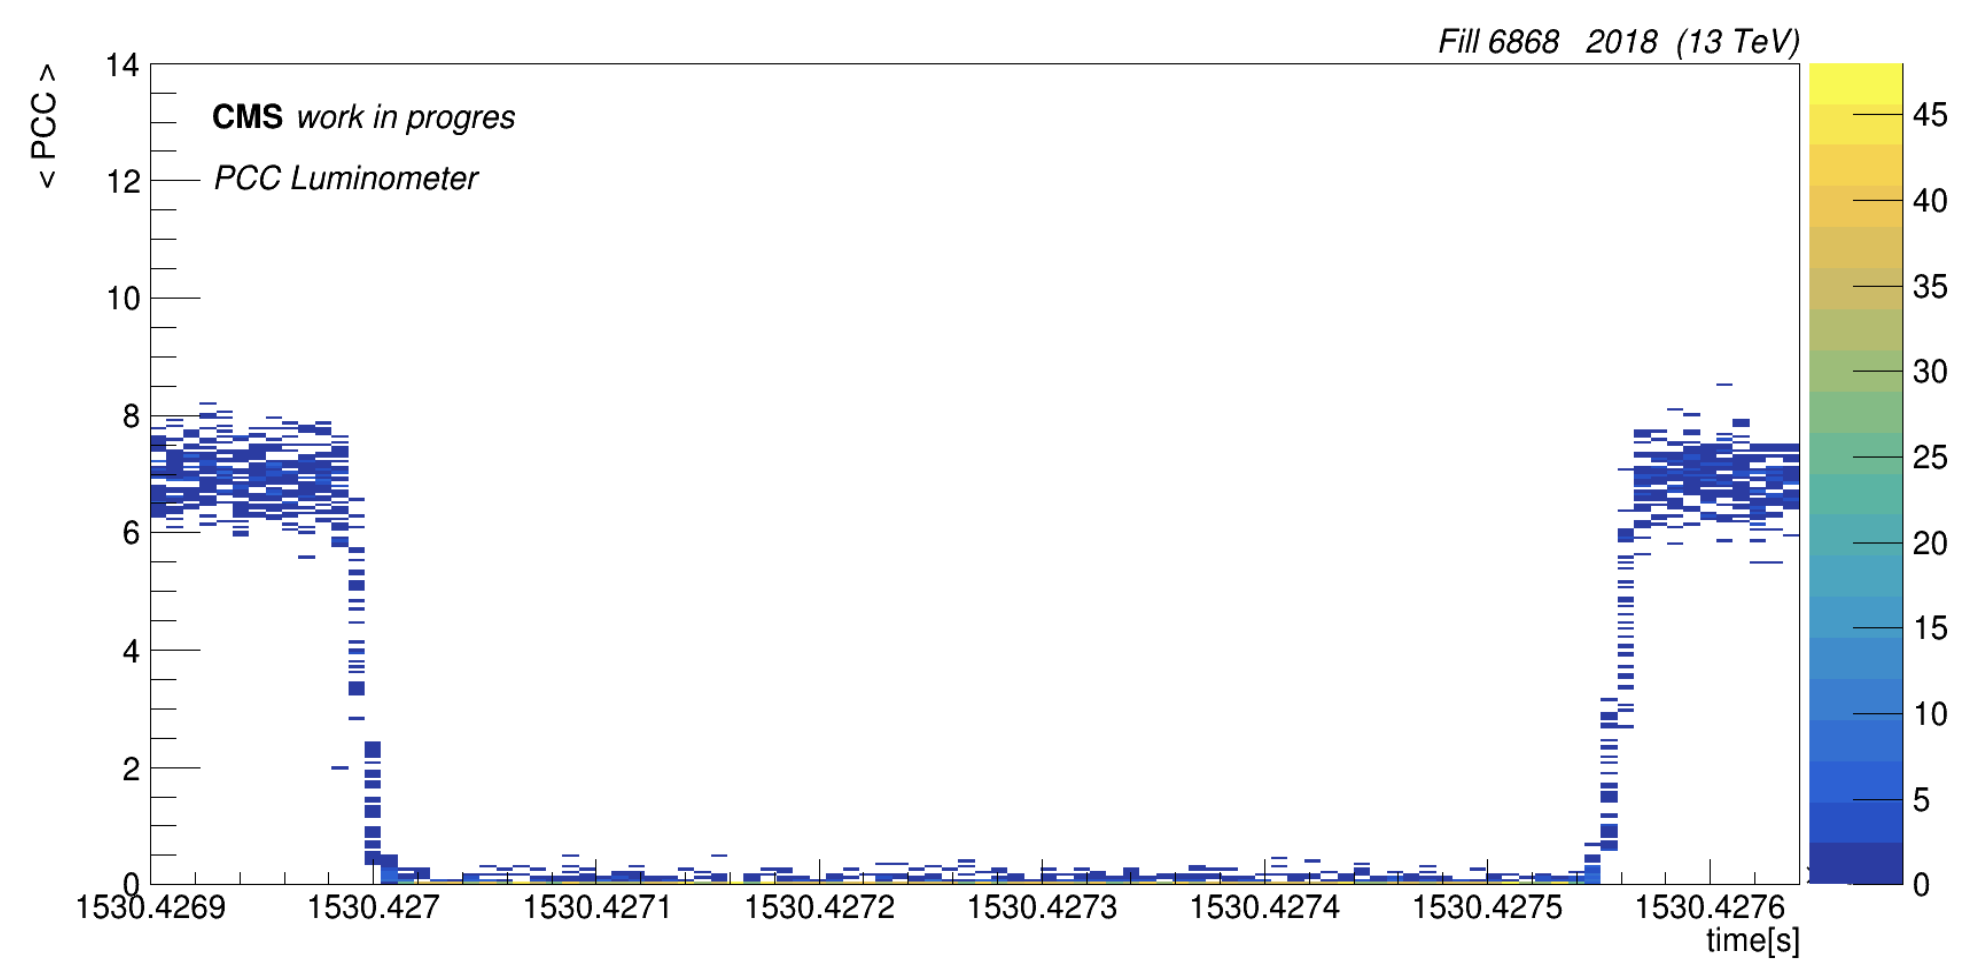
\includegraphics[width=1\textwidth]{ashish_thesis/SS1_SS2_bkg_pcc_1.png}
\caption[Background estimation]{2D histogram filled with the Avg. PCC evaluated per NB4, during head-on collisions (high part) and during the Super-Separation window (low part).}
\label{fig:sigmavis_ss_backg}
\end{figure}


\begin{table}
  \begin{center}
    \caption[2018 PCC Background]{Mean for the background estimated with the SS1 and SS2 data, separately for all five BCIDs and averaged.}
    \begin{tabular}{ccccc}
    \textbf{BCID}   & \textbf{Mean (SS1)} & \textbf{Mean (SS2)} \\ \hline
      265     &  0.02902    &  0.02743    \\
        865  &    0.02572  &     0.0281  \\
       1780    &  0.02862   &     0.0286  \\
       2192   &  0.02729  &     0.02323  \\
        3380  &  0.02882  &    0.02896   \\
      \end{tabular}
    %\caption[Background in PCC rate]{Mean for the background estimated with the SS1 and SS2 data, separately for all five BCIDs and averaged.}
    \label{tab:vdm:SS1_SS2}
  \end{center}
\end{table}

Figure \ref{fig:fitquality} displays the collision rates for a specific particle bunch as one beam is moved across another, with all necessary corrections applied. $\chi^2/ndof$ for vdM and imaging scans has an average value of 0.4514 where the Poly2G fit model converges for all BCIDs. Peak value and beam overlap $\Sigma_x$ and $\Sigma_y$ along X and Y are extracted from fit to calculate $\sigma_{vis}$. %The $\sigma_{vis}$ per scan is averaged over all BCIDs and its scan to scan variation is shown in Fig. \ref{fig:sigmaperscan}.
The $\sigma_{vis}$ value obtained by averaging all scans is for final module veto list is 960.54 $\pm$ 0.85(stat.) mb.

\begin{figure}[!htp]
    \centering
    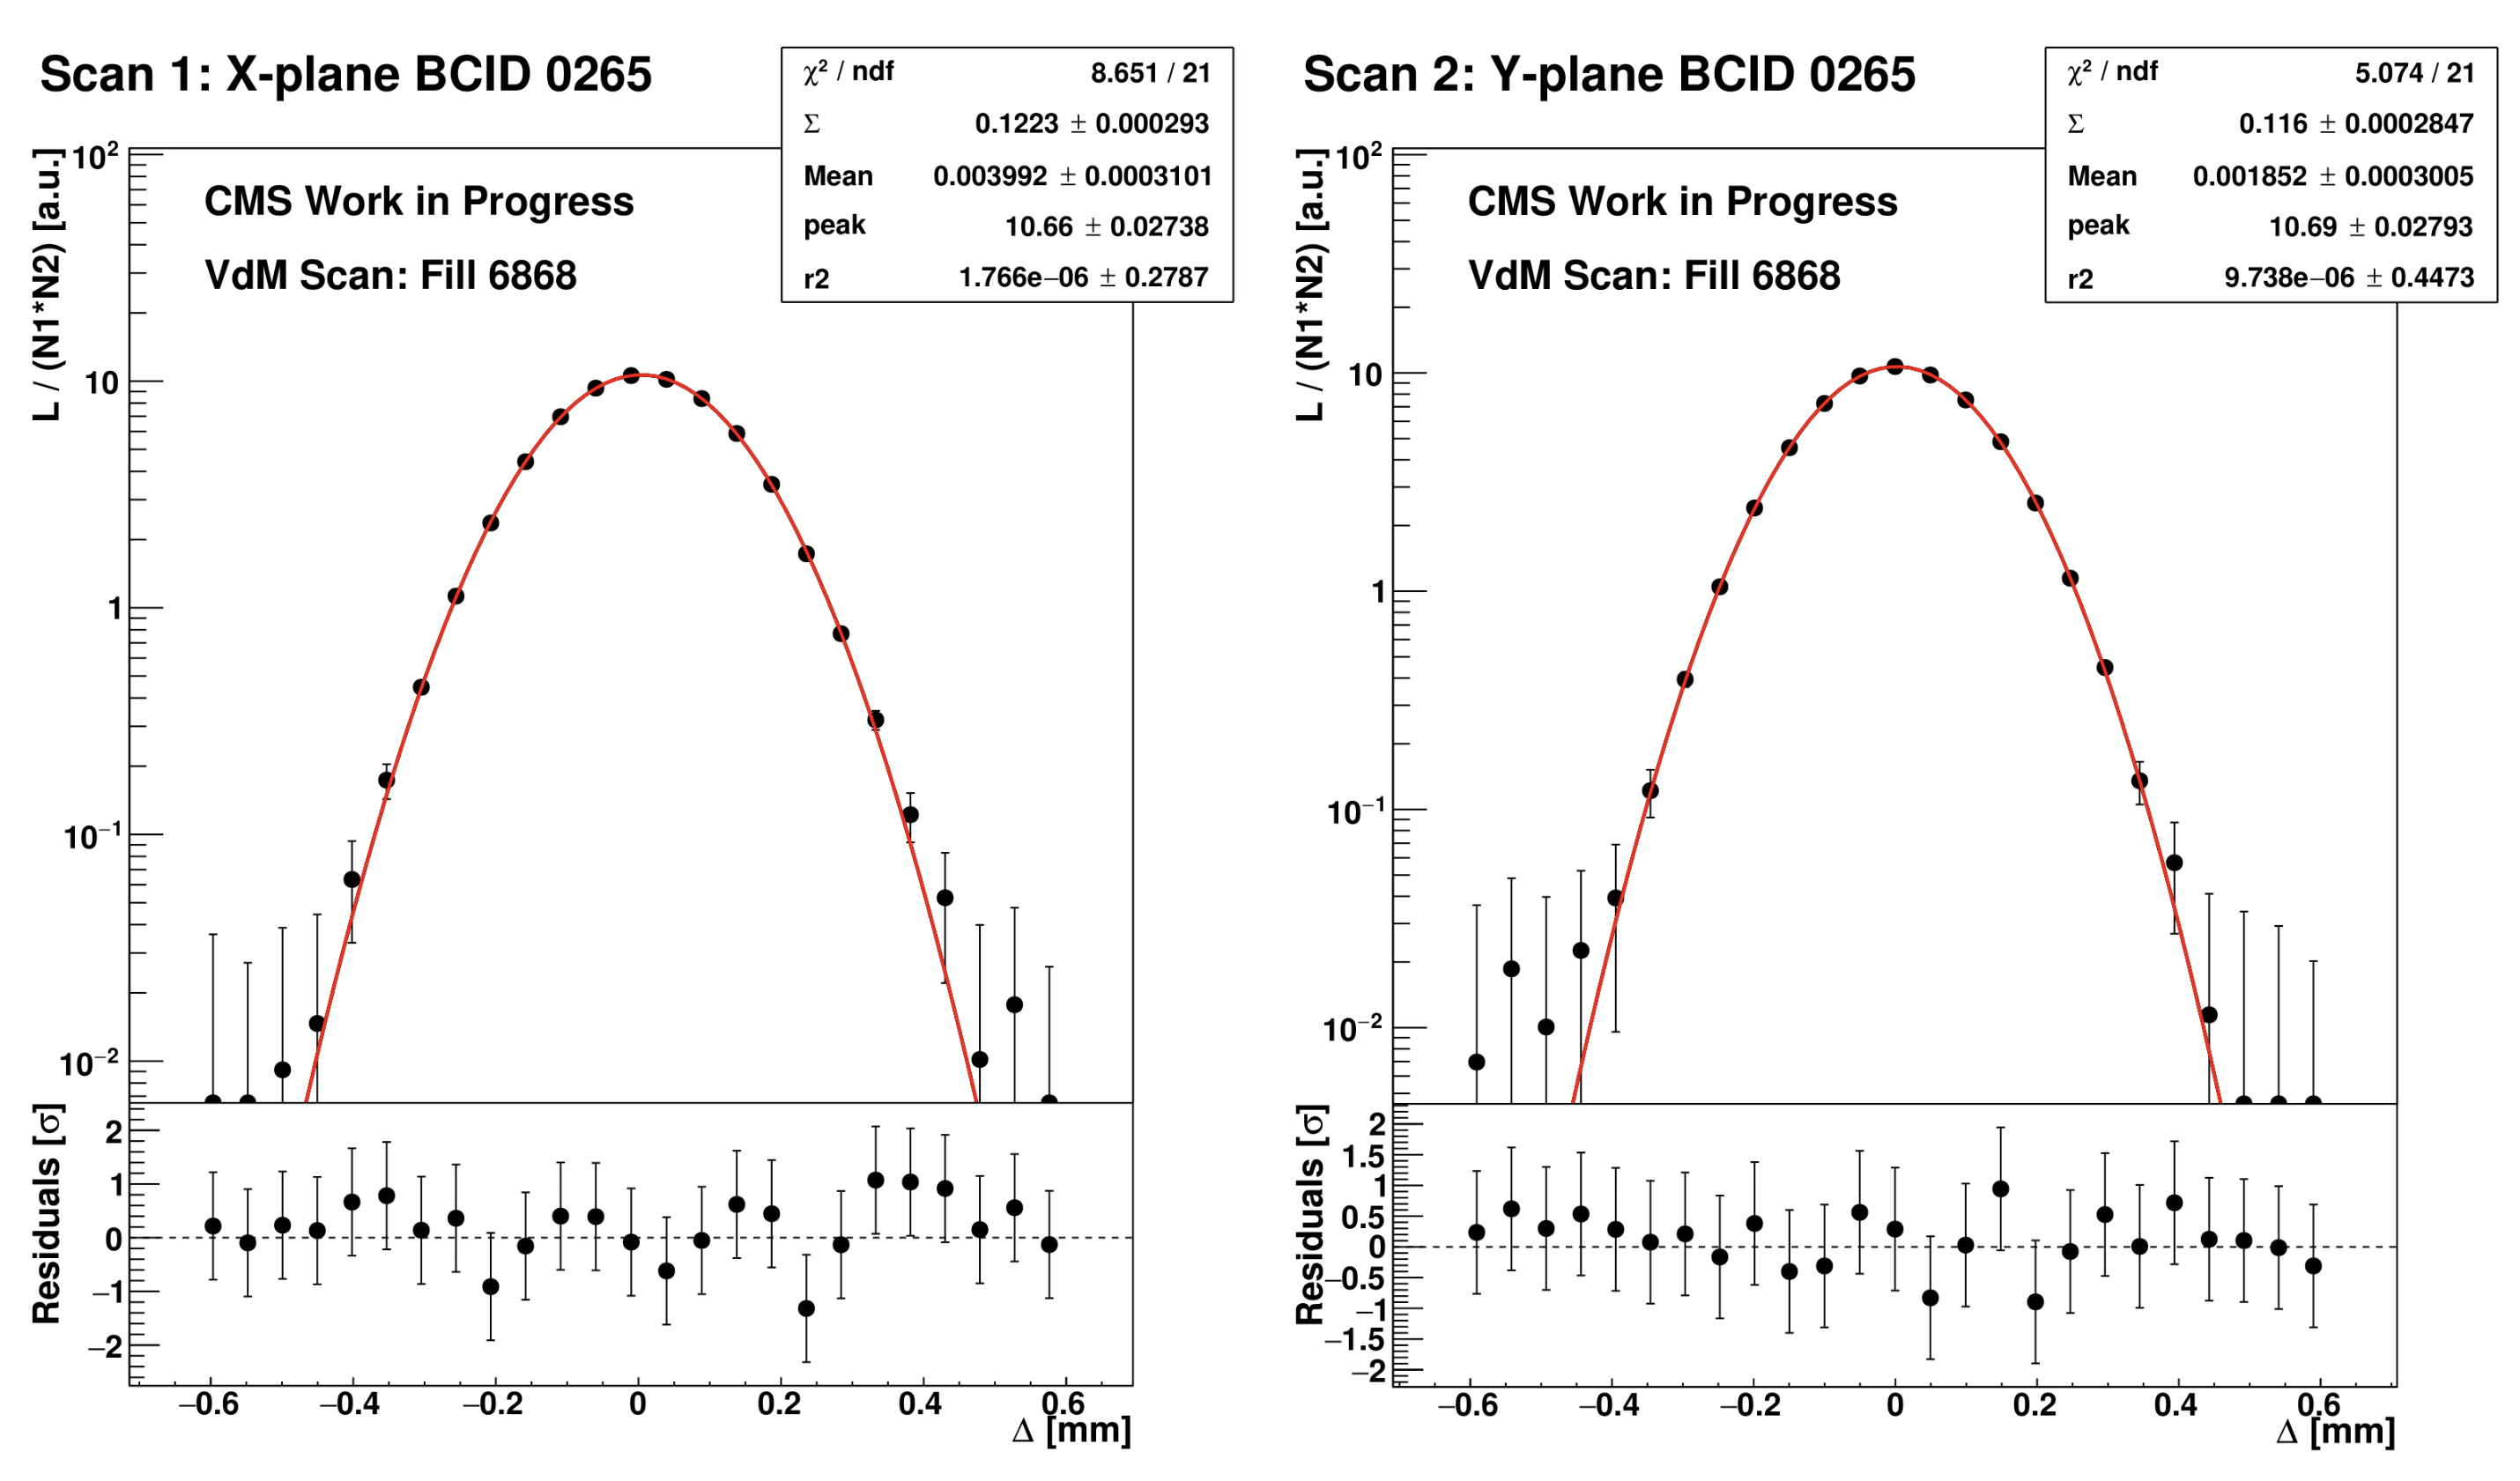
\includegraphics[width=1\textwidth]{ashish_thesis/vdM_fit_cveto_1.png}
    \caption[PCC Rate Fit]{Rates and the resulting fitted Poly2G scan curves as a function of the beam separation for a single bunch (BCID 265) as recorded by PCC for vdM1 scan in the x (left) and y direction (right). Background subtraction and the beam corrections have been applied to the raw data before the fit.}
    \label{fig:fitquality}
\end{figure}

%\begin{figure}[!htp]
 %   \centering
  %  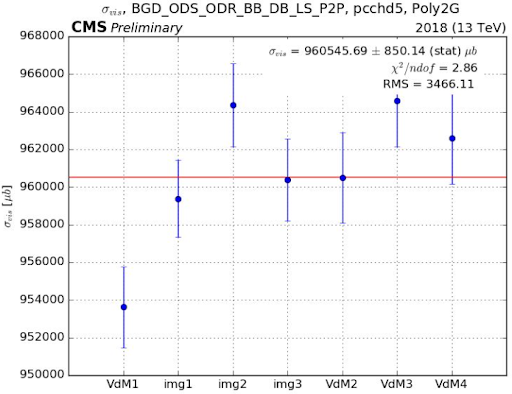
\includegraphics[width=0.8\textwidth]{ashish_thesis/sigma_vis_per_scan.png}
  %  \caption[PCC Visible Cross Section]{Visible cross section per scan where red line shows the average value.}
   % \label{fig:sigmaperscan}
%\end{figure}

PCC visible cross section for various bunch crossing across different scans is shown in Fig. \ref{fig:sigmavis_btob_variation}. The data points exhibit a scatter around the mean value, with no apparent systematic bias, as they are distributed both above and below this average. While there is a certain level of precision suggested by the proximity of the points to the mean line, the varying lengths of the error bars indicate a range in measurement uncertainty. This variability in precision could be attributed to fluctuating experimental conditions inherent to each BCID. %Overall, the experiment seems to have achieved a degree of accuracy, given that the measurements are clustered around the mean, yet the spread indicated by the error bars suggests that there is potential for optimizing the precision

\begin{figure}[!htp]
\centering
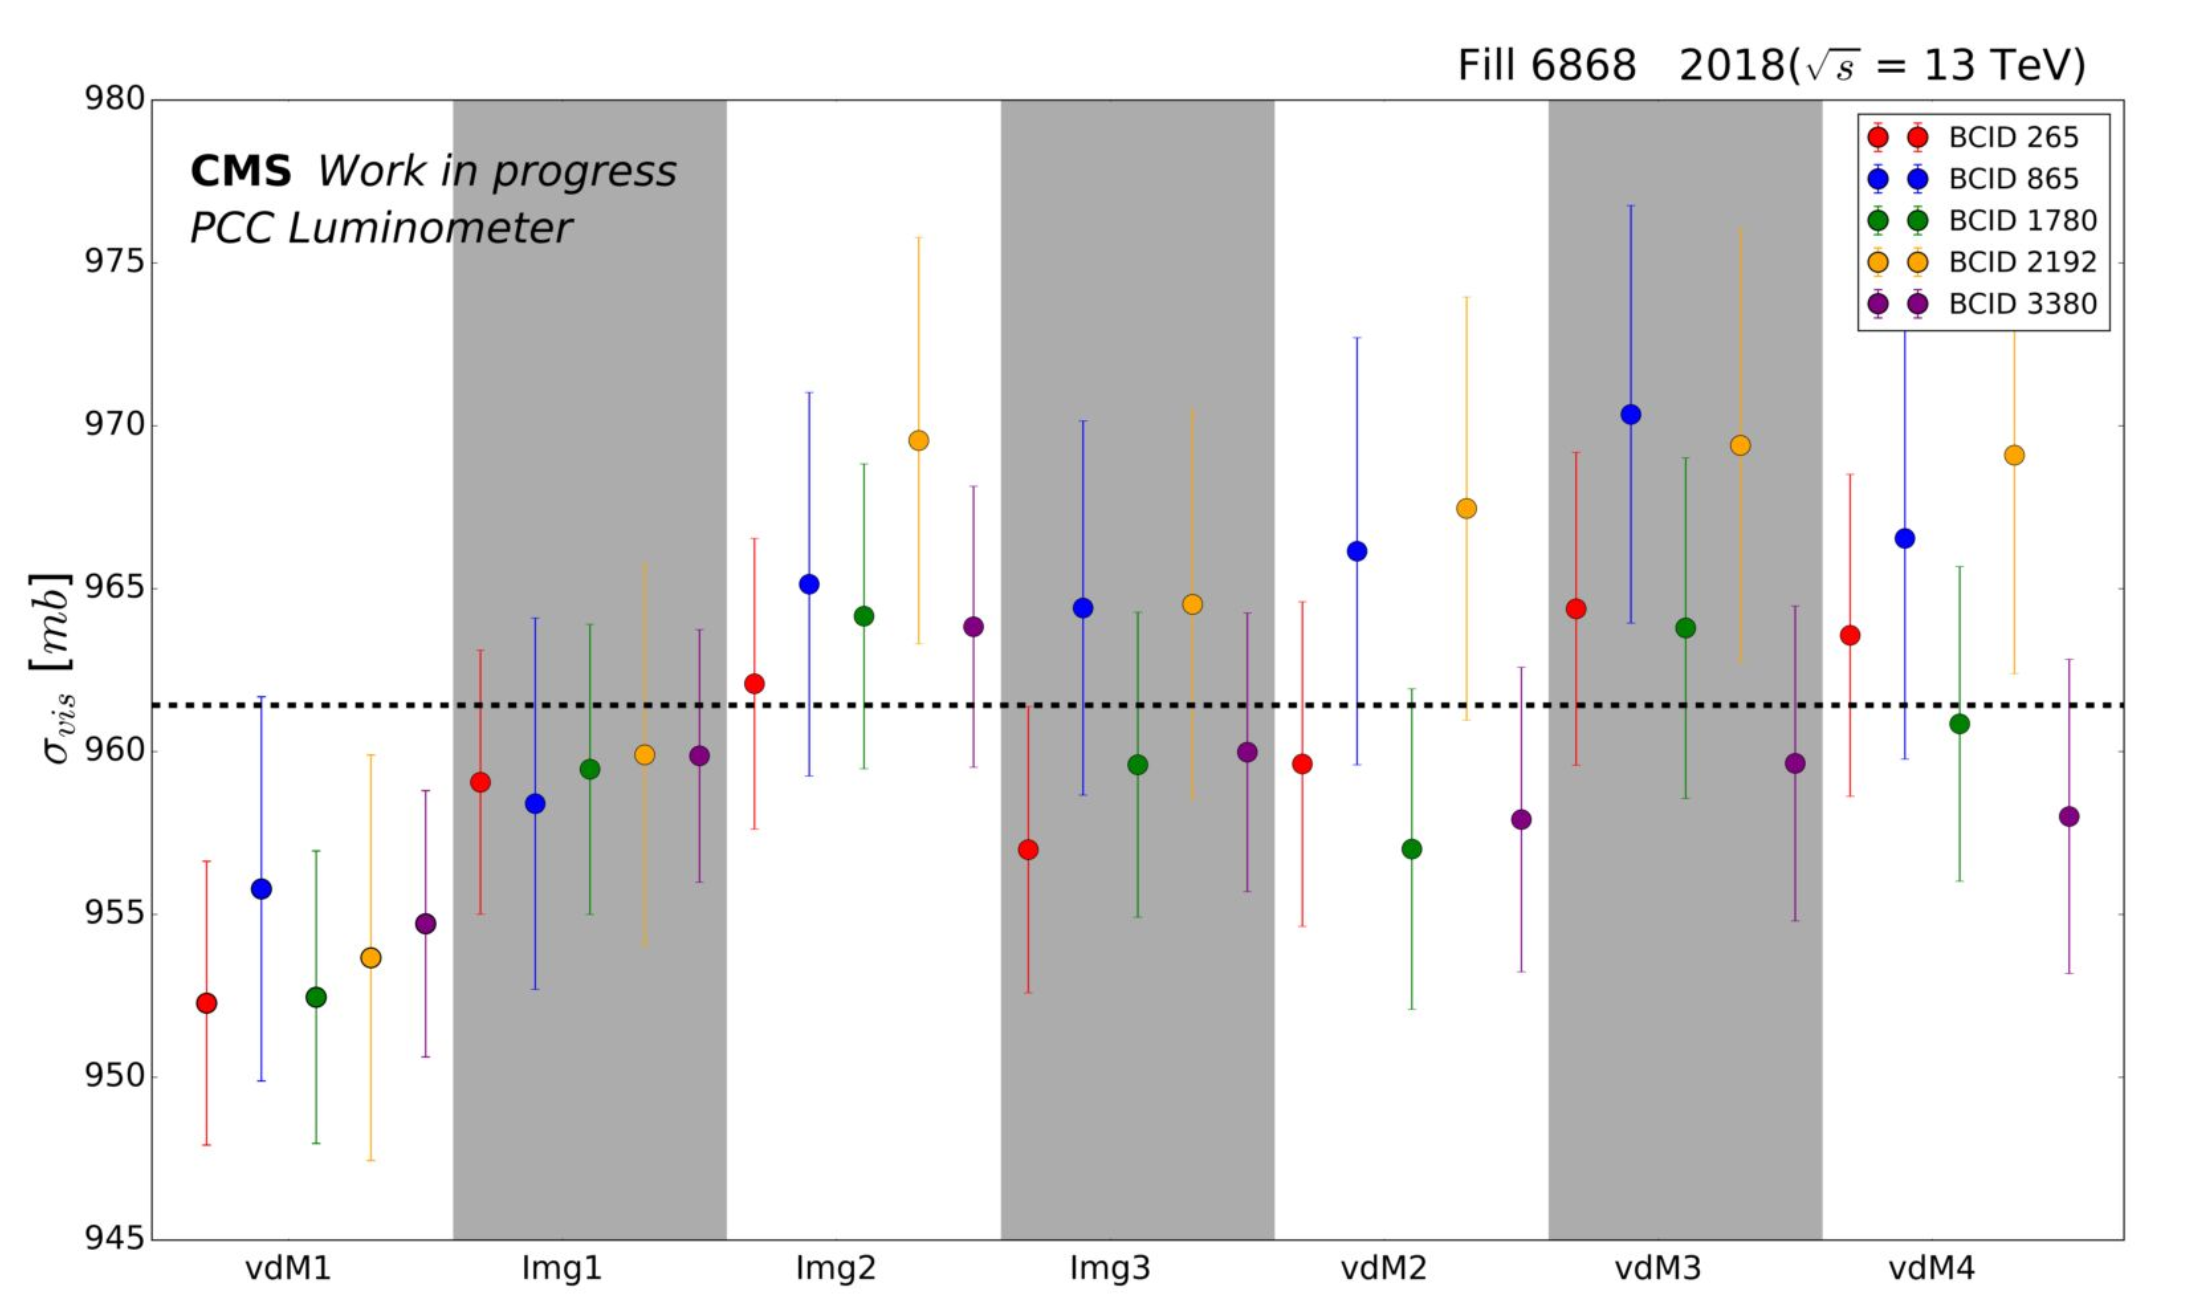
\includegraphics[width=0.7\textwidth]{ashish_thesis/sigma_vis_btob_var_1.png}
\caption[$\sigma_{vis}$ Bunch Variation]{%                                                                                                                                                       
 Bunch to bunch variation of PCC visible cross section.
}
\label{fig:sigmavis_btob_variation}
\end{figure}

\newpage
\section{Luminosity for physics fill}

The LHC operates in cycles known as "fills." A fill is a period during which the LHC is filled with protons and provides collisions for its experiments. The luminosity profile of a fill is a graphical representation of the instantaneous luminosity as a function of time for the entire duration of that fill. Before the actual data taking begins, there is a phase of beam injection, acceleration, and stabilization. During this period, no collisions are taking place, so the luminosity is zero. Once the beams are accelerated to their maximum energy and brought into collision, there is a rapid rise in luminosity. This is the point where the luminosity reaches its highest value, known as the peak luminosity. After the peak, the luminosity starts to decrease. This period, known as "stable beams", is when most of the data is collected. The reason for the decrease in luminosity over time is the reduction in the number of protons in the beams due to collisions. As the protons in the beams collide, the number of protons, and hence the luminosity, diminishes. The rate of this decrease can be influenced by various factors, including beam dynamics, losses, and the efficiency of the collider's operation. The fill concludes when the number of protons is too low to provide useful data, or if there's a technical issue, leading to a beam dump. At this point, the luminosity drops to zero. The total duration of a fill can vary. Some fills last only a few hours, while others can extend for over a day, depending on operational efficiency and the goals for that specific fill. Fill profile for Fill 6961 during 2018 data taking is shown in Fig. \ref{fig:Fill6961} with

\begin{itemize}
  
\item Peak luminosity = $1.85 \times 10^{34} cm^{-2} s^{-1}$
\item End luminosity = $0.9 \times 10^{34} cm^{-2} s^{-1}$ 
\item Number of colliding bunches = 2556
\item Number of lumi sections = 1400
\item Integrated luminosity = 0.418 $fb^{-1}$

\end{itemize}
    
\begin{figure}[!htp]
    \centering
    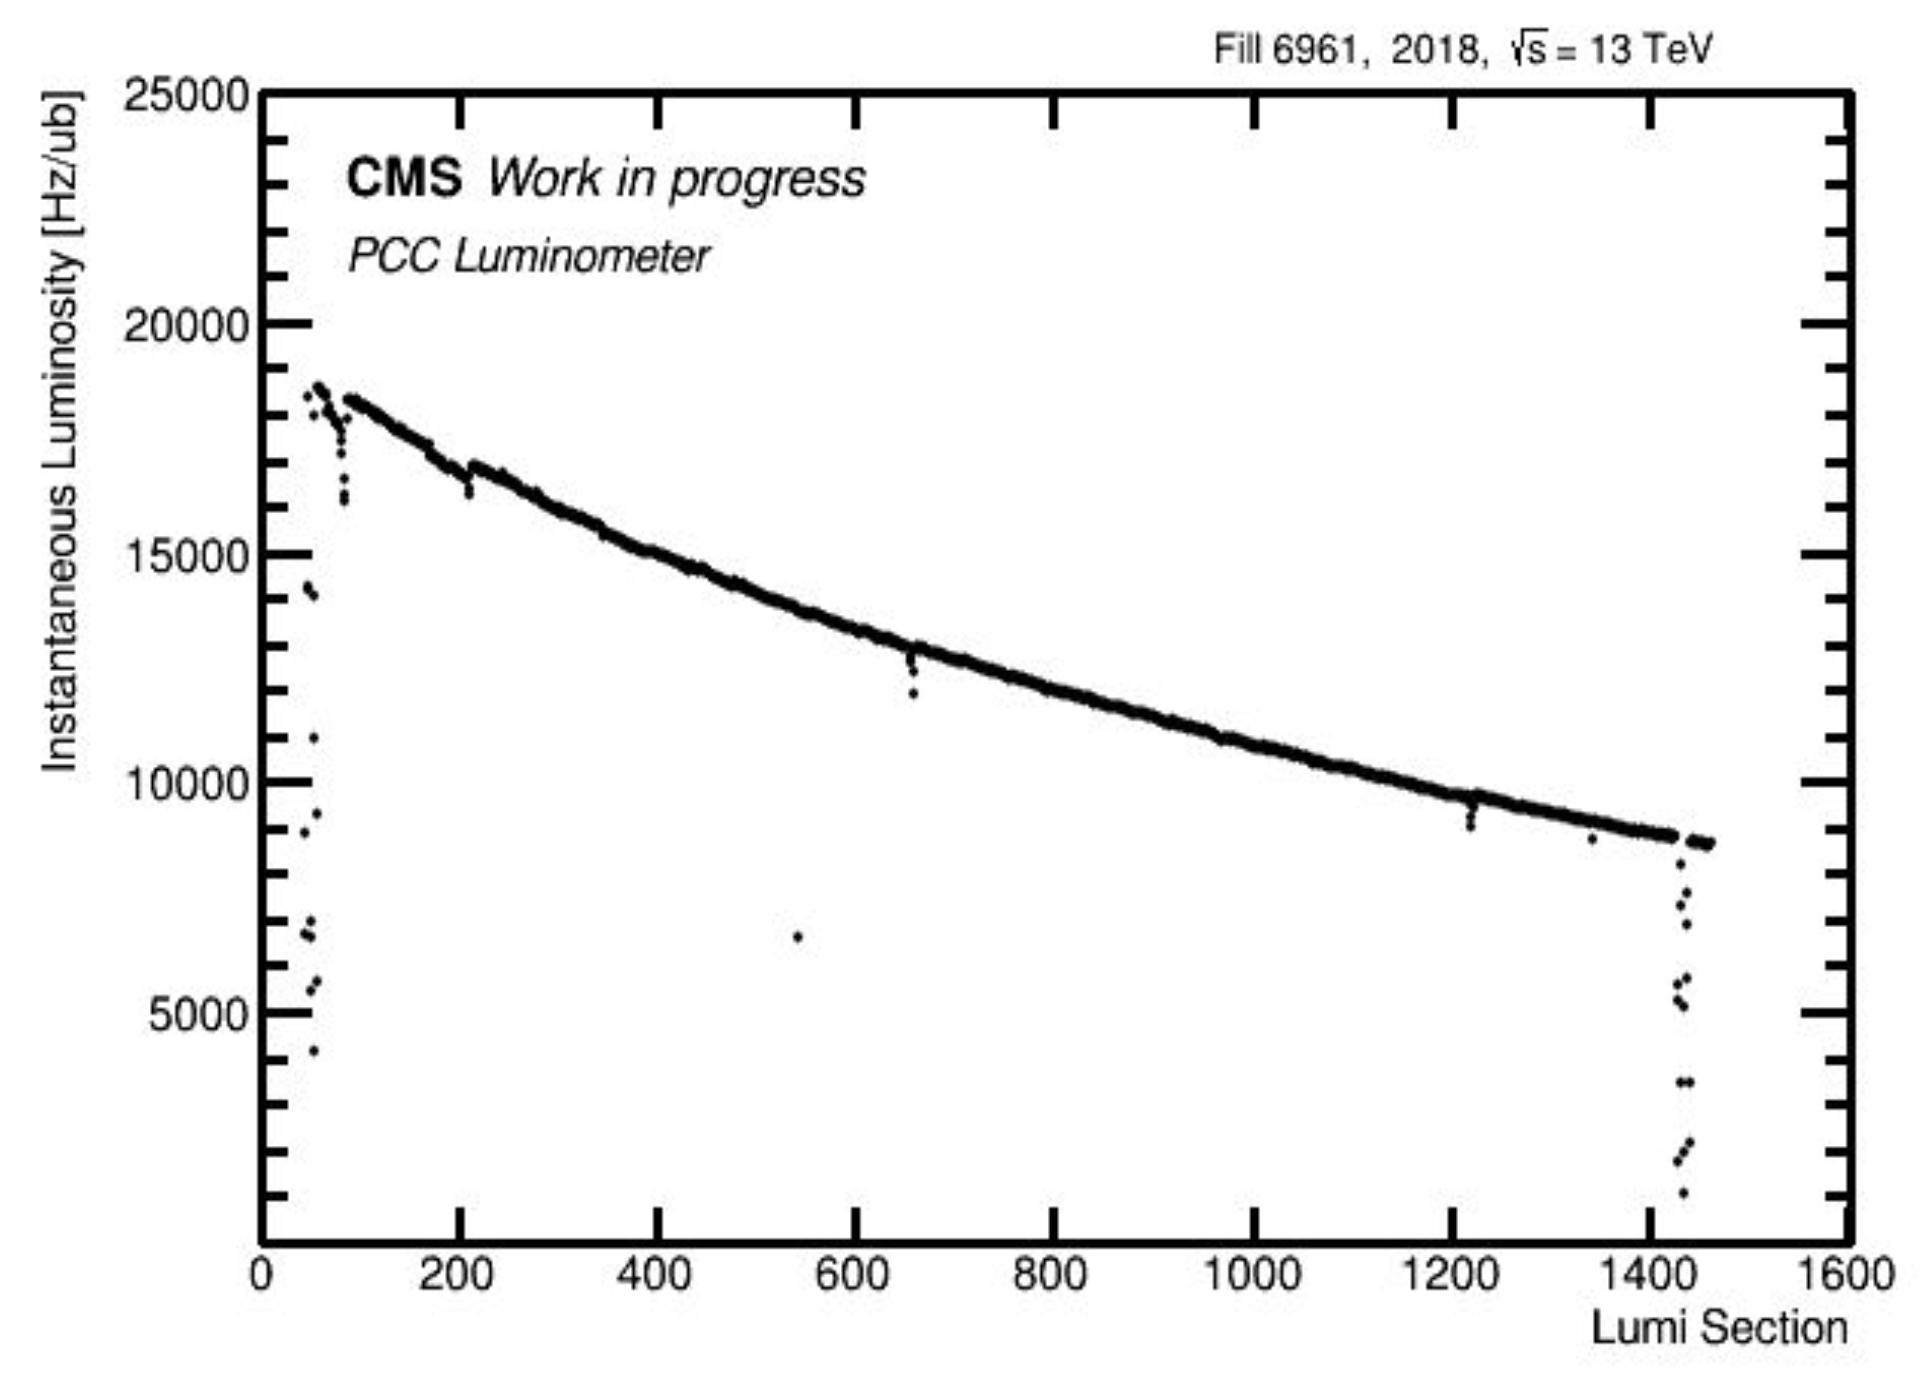
\includegraphics[width=0.9\textwidth]{ashish_thesis/Fill_profile_6961_1.png}
    \caption[Fill 6961 Profile]{Typical lumi profile for LHC Fill during 2018 data taking period for Fill 6961.}
    \label{fig:Fill6961}
\end{figure}


\newpage
\subsection{Afterglow backgrounds}

In the precision PCC luminosity measurement, understanding and rectifying the effects of afterglow is crucial. When estimating afterglow corrections, it's paramount to utilize raw PCC data obtained from both colliding and non-colliding bunches. The colliding bunches yield genuine signals representative of particle interactions, while the non-colliding bunches illuminate the background noise inherent in the system, simultaneously capturing any lingering afterglow from prior collisions. Two primary types of afterglow noise have been identified:

Type 1 Afterglow (Electronic Spillover): This noise arises due to the lingering signal waveform in silicon after an actual collision event.

Type 2 Afterglow (Activation-Induced Background): This noise is a consequence of the gradually diminishing activation of the detector. It occurs when the detector material encounters high-energy particles, leading to the creation and decay of radioactive isotopes \cite{CMS-PAS-SMP-12-008} %(as depicted in Fig. \ref{fig:pcc_afterglow}).

The afterglow correction process seeks to adjust for these residual signals, which result in background added to the cluster count. The concept of 'afterglow' is intrinsically tied to the detector and the events it records, independent of the specific modules used for data collection. Thus, regardless of any module's performance or operational state, the need for consistent afterglow correction remains.

In the afterglow correction process, following steps are involved.

\begin{itemize}
\item A model is constructed to mirror the afterglow tail from a single colliding bunch using the random trigger data.
\item The model is then fine-tuned according to the luminosity associated with that bunch.
\item In the ongoing correction process, a histogram representing the collision events and containing bunch trains is adjusted whereby the afterglow model, multiplied by the luminosity of each colliding pair, is subtracted from all subsequent collision events. This step ensures each bunch is comprehensively corrected.
\item Finally, the scale factor for correction is defined by the ratio of the corrected to the uncorrected PCC. This factor is then implemented in the final PCC for the ZB data. %An example plot of the scale factor is shown in Fig. \ref{fig:af_change_veto}.
\end{itemize}

Moreover, pedestal correction is essential. It signifies the adjustment of baseline values in the detector due to electronics noise. This procedure ensures accurate and stable readings from the pixel detector, culminating in precision PCC luminosity measurements. %An example of the afterglow correction factor including type 1, type 2 and pedestal corrections is shown in Fig. \ref{fig:af_change_veto}. 

For accurately modeling the afterglow effect in raw data, a composite function is utilized. It includes parameters for the Type 1 afterglow and an exponentially decaying model for Type 2, taking both amplitude and decay width into account. The model is summed over all bunch crossings.

\begin{equation}
F(x) = \sum_{k=0}^{N_{\text{bcid}}} N_k \left[ (x - k == 0) + A  (x - k == 1) + B  \exp(-C  (x - k - 1))  (x - k \geq 1) \right]
\end{equation}

Fill 9036, shown in \ref{fig:af_fit40} and encompassing 900 colliding bunches, serves as the foundation for estimating the Type 2 afterglow parameters. A fit is performed to one wagon train, then two, and finally three, refining the parameters for Type 2 afterglow and minimizing the residuals of both afterglow types. Fit plots for single train is shown in \ref{fig:af_fit99}. The values of type 2 afterglow parameter amplitude (B) and decay width (C) for different wagon trains are shown in Table \ref{fig:af_fit4000}. 

\begin{comment}

Type 1 and Type 2 afterglow corrections are very important for precise PCC luminosity measurement. Type 1 afterglow noise, or electronic spillover, arises due to the lingering signal waveform within silicon after actual collision event. Contrarily, Type 2 afterglow noise emanates from the exponentially diminishing activation of the detector caused by the creation of secondary particles when the detector material encounters high-energy particles \cite{CMS-PAS-SMP-12-008} (as depicted in Fig. \ref{fig:pcc_afterglow}).

The rectification of afterglow noise is achieved by constructing a model that replicates the tail of the afterglow from a single collision event. This model is then adjusted according to the luminosity of the event. In an ongoing process of correction, a histogram representing the collision events and containing bunch trains is adjusted, whereby the afterglow model is multiplied by the luminosity of each colliding pair and subsequently deducted from all subsequent collision events. This iterative process is repeated for all colliding pairs, ensuring each event is completely rectified prior to being used for further correction.

The afterglow correction, or the scale factor, is determined by calculating the ratio of the corrected to uncorrected PCC. This factor is then implemented into individual event histograms within the zero bias data.

%The afterglow correction is independent of the module veto list as shown in Fig. \ref{fig:af_change_veto} , meaning the correction is applied universally across all modules irrespective of whether a module is on the veto list or not. This is because afterglow is a characteristic of the detector material and particle interactions, not of the specific modules. Thus, even when the module veto list changes, the afterglow corrections remain consistent, ensuring accurate luminosity measurement.

The afterglow correction in PCC luminosity measurement is a compensatory procedure that's designed to adjust for the lingering effects of prior particle collisions, which may otherwise skew the accuracy of the luminosity calculations. The concept of 'afterglow' is related to these residual signals, identified as Type 1 and Type 2, that originate from the detector material and the physical processes associated with the particle interactions. Importantly, the presence and extent of afterglow are influenced by these fundamental factors and are not dictated by the operational state or quality of any individual detector module as shown in Fig. \ref{fig:af_change_veto}. That is, the afterglow is an inherent characteristic tied to the detector and the physical event, and it is independent of the specific modules being used to collect the data. A module veto list is a register of detector modules that are excluded from data collection and analysis for various reasons, such as suboptimal performance, high noise levels, or other technical issues. When a module is added to or removed from the veto list, it can affect the raw data that's being gathered, but it doesn't influence the underlying afterglow characteristics that are tied to the detector material and the particle collisions. Therefore, changes to the veto list do not alter the need for, or the application of, the afterglow correction. Consequently, the afterglow correction process remains consistent and is applied across all modules, irrespective of their veto list status. This ensures that the measured luminosity accurately represents the actual particle collision events, providing reliable data for subsequent analysis and interpretation, regardless of the specific module configuration at any given time.

Apart from afterglow corrections, pedestal correction is another critical component. It signifies the adjustment of baseline values in the detector readout to account for any systematic biases or drifts. The pedestal correction involves monitoring the detector's output in the absence of a signal, and then subtracting this baseline value from the signal collected during data capture. The application of pedestal correction significantly enhances the accuracy and stability of the pixel detector's readings, thereby leading to precision measurement of PCC luminosity.

\newpage
\begin{figure}[H]
\centering
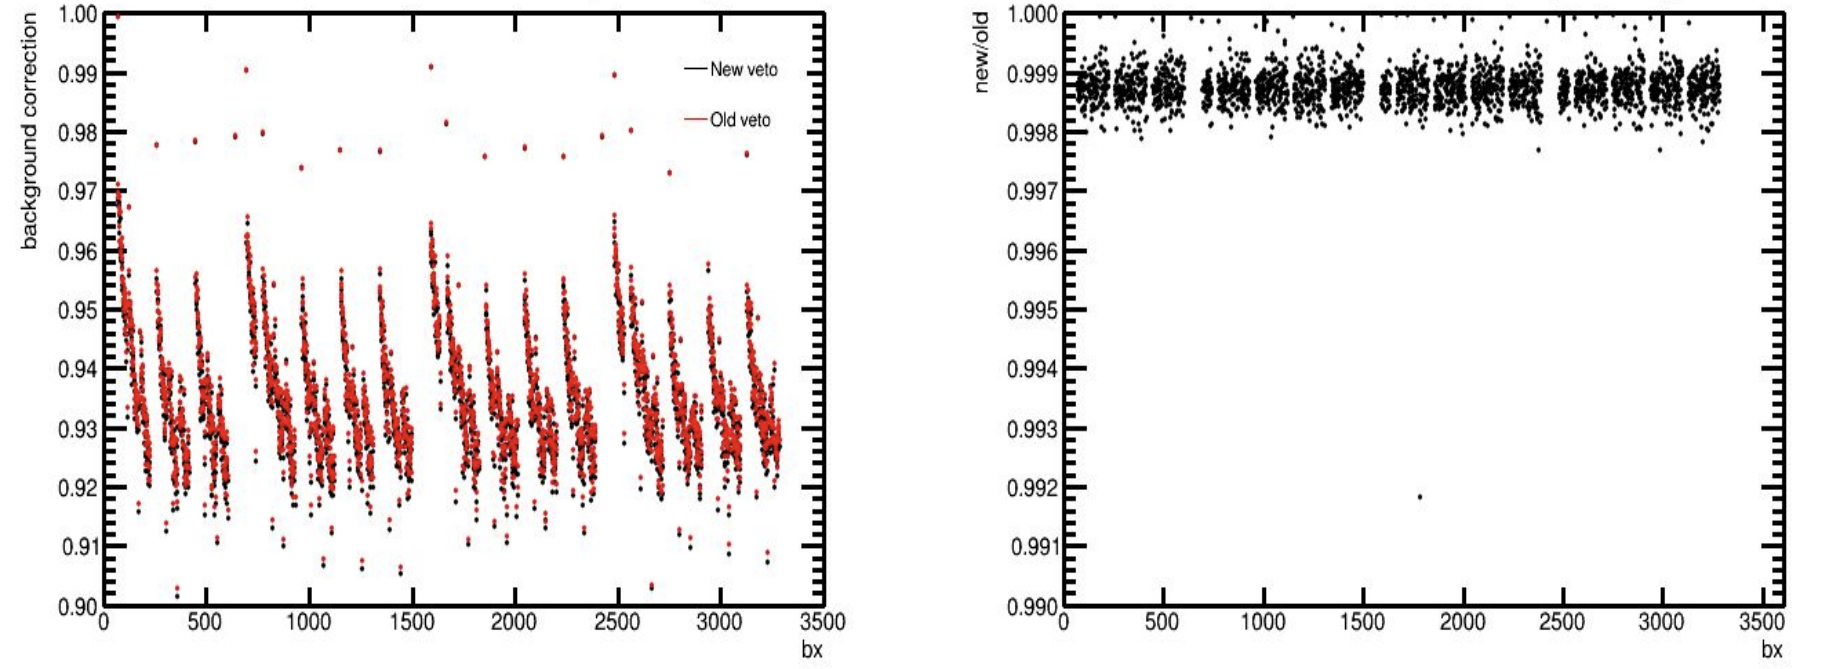
\includegraphics[width=0.7\textwidth]{ashish_thesis/veto_change_same_af.png}
\caption[Afterglow background ratio]{%                                                                                                                                                                         
    Ratio of afterglow scale factor for new per period veto and old veto.
}
\label{fig:af_change_veto}
\end{figure}

%Type 1 and Type 2 afterglow corrections are essential for obtaining accurate PCC measurements. Type 1 afterglow noise, also known as electronic spillover, is caused by the long waveform of the signal in silicon. On the other hand, Type 2 afterglow noise is the exponentially decaying detector activation due to the production of secondary particles when high-energy particles interact with the detector material as shown in Fig. \ref{fig:pcc_afterglow}. Afterglow noise is corrected by creating a model of the afterglow tail of a single colliding bunch, which is then normalized to the luminosity of the colliding bunch crossing. A bunch-by-bunch histogram containing bunch trains undergoes afterglow correction, where the afterglow model is multiplied with the luminosity of each colliding bunch pair and subsequently subtracted from all following bunches. This correction process is performed iteratively for all colliding bunch pairs, ensuring that a given bunch crossing is fully corrected before being used to correct the subsequent bunch crossings. The afterglow correction, or scale factor, is calculated by taking the ratio of the corrected and uncorrected PCC. This scale factor is then applied to individual bunch-by-bunch histograms in the zero bias data. In addition to afterglow corrections, pedestal correction is another important aspect to consider. Pedestal correction refers to the adjustment of baseline values in the detector readout to account for any systematic offsets or drifts. This process involves measuring the detector's output when no signal is present and subtracting this baseline value from the measured signal during data collection. By performing pedestal correction, the accuracy and stability of the detector's measurements are significantly improved, contributing to more reliable PCC measurements.

%Type 1 and 2 afterglow corrections are measured and applied to the PCC measurement. Type 1 afterglow noise is electronic spillover due to long waveform of the signal 549 in silicon and Type 2 afterglow noise is exponentially decaying detector activation due to production of secondary particles when high energy particles interact with detector material as shown in Fig. 15. Afterglow noise is corrected by making a model of afterglow tail of a single colliding bunch, normalized to the luminosity of the colliding bunch crossing. Bunch-by-bunch histogram containing bunch trains is corrected for afterglow where afterglow models is multi554 plied with the luminosity of each colliding bunch pair and subtracted from all following bunches. This correction is performed iteratively over all colliding bunch pairs such that a given bunch crossing is fully corrected before it is used to correct the succeeding bunch crossings. The afterglow correction (or scale factor) can be calculated by taking the ratio of corrected and uncorrected PCC. This scale factor is applied to individual bunch-by-bunch histograms in the zero bias data.

\begin{itemize}

\item Type 1 afterglow correction: Type 1 afterglow refers to the residual signals in the detector caused by particles from previous bunch crossings. These particles can be trapped in the detector's sensitive volume, leading to an overestimation of the actual number of pixel clusters. The Type 1 afterglow correction aims to correct for this by subtracting the expected contribution of these residual signals from the raw PCC data.

\item Type 2 afterglow correction: Type 2 afterglow is associated with the activation of detector material due to high-energy particle interactions. When high-energy particles interact with the detector material, they can cause the material to become radioactive. The decay of these radioactive isotopes produces additional signals in the detector, which can lead to an overestimation of the number of pixel clusters. The Type 2 afterglow correction aims to account for these additional signals by subtracting the expected contribution of the activation-induced background from the raw PCC data.

\item Pedestal correction: The pedestal correction refers to the baseline noise level in the detector, which can be influenced by factors such as temperature fluctuations, electronic noise, and radiation damage. This noise can cause an over- or underestimation of the actual number of pixel clusters. The pedestal afterglow correction aims to correct for this by adjusting the raw PCC data based on a measurement of the pedestal noise level.

\end{itemize}

\end{comment}

%The scale factor for one 50 lumi section block in run number 315690 is shown in Fig. \ref{fig:af_change_veto}. It provides an overview of the afterglow scale factor applied to the raw PCC. On the left, both the raw and corrected PCC for all bunch crossings are displayed, showing the variations between the initial data and the adjusted counts. The right side specifically highlights the afterglow scale factor for a single 50 lumi section block, representing the afterglow correction applied for final module veto. 

%\begin{figure}[!htp]
%\centering
%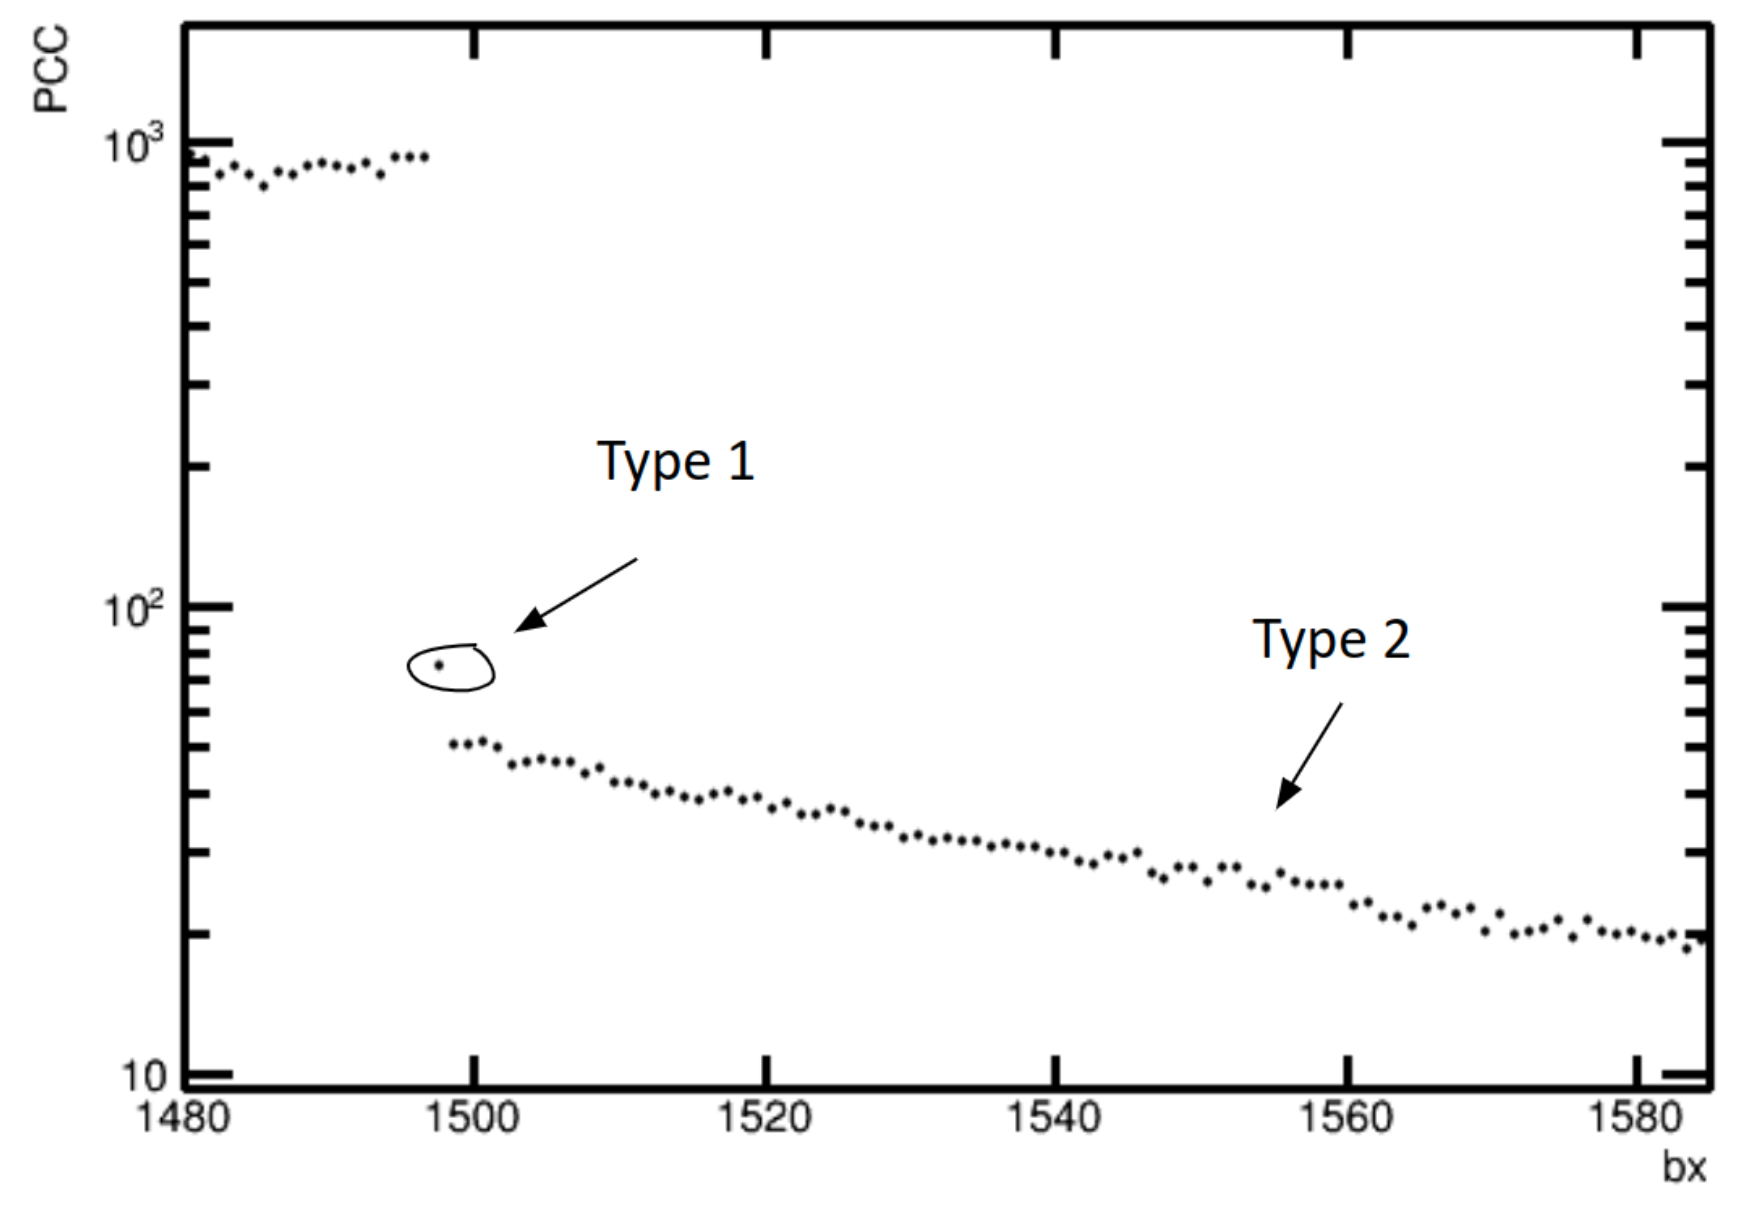
\includegraphics[width=0.7\textwidth]{ashish_thesis/af_t1_t2.png}
%\caption[Afterglow Effect Single Bunch]{%
%Afterglow corrections are calculated from cluster rate measurements in empty bunches. Electronic spillover (“Type-1”). Type-1 noise is due to long waveform of the signal in silicon. First empty bunch after bunch train is used to calculate it. Exponentially decaying detector activation (“Type-2”).  Type-2 noise is due to production of secondary particles when high energy particles interact with detector material. All empty bunches after bunch train are used to calculate it.
%}
%\label{fig:pcc_afterglow}
%\end{figure}


%\begin{figure}[!htp]
%\centering
%\includegraphics[width=1\textwidth]{ashish_thesis/afterglow_correction_factor_1lsblock_315690.png}
%\caption[Afterglow background]{%                                                                                                                                                                                          
% Left: Raw and corrected PCC for all bunch crossings. Right: Afterglow scale factor for one 50 lumi section block in run 315690 for the final module veto.
%}
%\label{fig:af_change_veto}
%\end{figure}

\begin{comment}

The model used for fitting the afterglow in PCC raw data consists of a parameter for type 1 afterglow correction and exponentially decaying model with two parameters for type 2 afterglow correction taking into account amplitude and decay width. The fit function is summed over all bunch crossings. Fill 9036 (shown in Fig. \ref{fig:af_fit40}) consisting of 900 colliding bunches is used for the estimation of type 2 afterglow parameters. We start by fitting a single 50 lumi section block, then fit one wagon train, two wagon train and three wagon train to get better estimation of type 2 afterglow parameters to obtain least type 1 and type 2 afterglow residuals. 

\end{comment}

\newpage
\begin{figure}[H]
\centering
\includegraphics[width=0.8\textwidth]{ashish_thesis/fill_7036_pattern_2.png}
\caption[7036 Fill Patern]{%                                                                                                                                                                                         
  Fill 7036 pattern (900 b fill).
}
\label{fig:af_fit40}
\end{figure}

%Fit plots for single 50 lumi section block, 2 wagon and 3 wagon trains are shown in Fig. \ref{fig:af_fit41}, \ref{fig:af_fit} and \ref{fig:af_fit99}.



%\begin{figure}[!htp]
%\centering
%\includegraphics[width=1\textwidth]{ashish_thesis/af_model_fit.png}
%\caption[]{%                                                                                                                                                                                                         
 % Afterglow fit model for single 50 lumi section block.
%}
%\label{fig:af_fit41}
%\end{figure}


%\begin{figure}[!htp]
%\centering
%\includegraphics[width=1\textwidth]{ashish_thesis/bunch_train.png}
%\caption[]{%                                                                                                                                                                                  
                                                                                                                                                                                       
  %Afterglow fit model.
%}
%\label{fig:af_fit}
%\end{figure}



%\begin{figure}[!htp]
%\centering
%\includegraphics[width=1\textwidth]{ashish_thesis/2wagon_af.png}
%\caption[]{%                                               
                                                                                                                                   
 % Afterglow fit model.
%}
%\label{fig:af_fit}
%\end{figure}

%\begin{figure}[!htp]
%\centering
%\includegraphics[width=1\textwidth]{ashish_thesis/2wagon_fit.png}
%\caption[]{%                                                                                                                                 
 % Afterglow fit model for 2 wagon train.
%}
%\label{fig:af_fit}
%\end{figure}


%\begin{figure}[!htp]
%\centering
%\includegraphics[width=1\textwidth]{ashish_thesis/3wagon_af.png}
%\caption[]{%                                                                                  
                                                                                                                                                                                                                                     
 % Afterglow fit model.
%}
%\label{fig:af_fit}
%\end{figure}

%\begin{figure}[!htp]
%\centering
%\includegraphics[width=1\textwidth]{ashish_thesis/3wagon_fit.png}
%\caption[Afterglow Fit]{%                                                                          
 % Afterglow fit model for 3 wagon train.
%}
%\label{fig:af_fit99}
%\end{figure}

\begin{figure}[H]
  \centering
    \includegraphics[width=0.75\textwidth]{ashish_thesis/2018_af_fit_1.png} 
  %\hfill % or \hspace{5mm} for a specific horizontal space                                                                                                  
  %\begin{subfigure}[b]{0.49\textwidth}
   % \includegraphics[width=\textwidth]{ashish_thesis/2018_af_fit_residuals.png}                                                                                     
  %\end{subfigure}
  \caption[Afterglow Effect Fit]{Fit to single train to estimate afterglow parameters.}
  \label{fig:af_fit99}
\end{figure}

%\begin{figure}[!htp]
%\centering
%\includegraphics[width=1\textwidth]{ashish_thesis/type2_af_parameters.png}
%\caption[]{%                                                                                
 % Afterglow fit model.
%}
%\label{fig:af_fit}
%\end{figure}

%The values of type 2 afterglow parameter amplitude (a) and decay width (b) for different wagon trains are shown in Table \ref{fig:af_fit4000}.

\newpage
\begin{table}
  \centering
  \caption[Type 2 afterglow parameters estimation]{Type 2 afterglow parameters obtained from fit to raw pcc data}
  \begin{tabular}{ccc}
    \textbf{\# of wagon} & \textbf{B} & \textbf{C} \\
     \hline
   %1-wagon train  & 0.001246  & 0.01261 \\
   2-wagon train  & 0.000813 &  0.01219\\
   3-wagon train  & 0.0008265 &  0.01231\\
  \end{tabular}
  %\caption{Type 2 afterglow parameters obtained from fit to raw pcc data}
  \label{fig:af_fit4000}
\end{table}

The scale factor for one 50 lumi section block in run number 315690 is shown in Fig. \ref{fig:af_change_veto}. It provides an overview of the afterglow scale factor applied to the raw PCC. On the left, both the raw and corrected PCC for all bunch crossings are displayed, showing the variations between the initial data and the adjusted counts. The right side specifically highlights the afterglow scale factor for a single 50 lumi section block, representing the afterglow correction applied for final module veto.

\newpage
\begin{figure}[H]
\centering
\includegraphics[width=0.8\textwidth]{ashish_thesis/afterglow_correction_factor_1lsblock_315690_2.png}
\caption[Run 315690 Afterglow Background]{%                                                                                                                                                                                                                                                                                                
 Raw and corrected PCC for all bunch crossings.
}
\label{fig:af_change_veto}
\end{figure}

\begin{figure}[H]
\centering
\includegraphics[width=0.8\textwidth]{ashish_thesis/afterglow_correction_factor_1lsblock_315690_3.png}
\caption[Run 315690 Afterglow Background]{%
  Afterglow scale factor for one 50 lumi section block in run 315690 for the final module veto.
}
\label{fig:af_change_veto}
\end{figure}


\section{PCC instantaneous and integrated luminosity}

Instantaneous luminosity is proportional to the rate of collisions at any given moment in time. It is a snapshot of the experiment's performance and is represented as \( L_{\text{inst}} \). The unit of instantaneous luminosity is often Hertz per micro barn $(Hz/ub)$. Integrated luminosity is the accumulation of instantaneous luminosity over a specific time period. Mathematically, it is defined as:
\[
\text{Integrated Luminosity} = \int (\text{Instantaneous Luminosity}) \, dt
\]
The unit of integrated luminosity is typically inverse femtobarns (\( \text{fb}^{-1} \)). Integrated luminosity can be understood as the sum of all instantaneous luminosities over the duration of the experiment, enhancing the statistical significance of the data collected. It serves as a measure of the total number of events recorded by the experiment, crucial for robust statistical analysis. When plotted as a function of lumi sections, PCC instantaneous and integrated luminosity offer distinct yet complementary insights into the experiment's performance. In plots that feature luminosity as a function of these lumi sections, the x-axis enumerates the lumi sections while the y-axis presents the luminosity values.  For instantaneous luminosity, discrete data points are plotted for each lumi section, providing immediate, lumi section specific measurements of the collision rate as shown in Fig. \ref{fig:PCC_inst_2018}. These points can fluctuate based on a variety of factors, such as beam conditions or adjustments to the accelerator. On the other hand, integrated luminosity is represented by a continuously ascending curve. %Each point on this curve accumulates the instantaneous luminosity values up to that specific lumi section. %The integrated luminosity for entire 2018 is calculated to be 60.47 fb^{-1}.

\begin{figure}[!htp]
\centering
\includegraphics[width=1\textwidth]{ashish_thesis/PCClumivslumisection_2018_1.png}
\caption[2018 PCC Inst. Luminosity]{%                                                                                                                                                                   
 2018 PCC instantaneous luminosity as a function of lumi section.
}
\label{fig:PCC_inst_2018}
\end{figure}

\newpage
\section{Systematic uncertainties}

The luminosity measurement at CMS experiment is influenced by various systematic uncertainties. Systematic uncertainty originates from inherent biases in experimental design, instrumentation, or methodologies, consistently skewing results away from the true value. These include effects from orbit drifts, xy non-factorization, beam-beam interactions, stability issues, non-linearity of the detector response, afterglow from preceding collisions, and CMS deadtime. Each of these sources can impact the precision of the luminosity determination and requires careful consideration in the luminosity's data analysis.

\subsection{vdM calibration uncertainties}

\begin{itemize}

\item Orbit Drift: Orbit drift in particle accelerators refers to the slight deviation or shift in the trajectory of circulating particle beams from their intended path. This drift can be caused by a myriad of factors, including imperfections in the magnetic fields guiding the beams, external disturbances, and even minute ground movements or temperature fluctuations affecting the accelerator components. The precision with which beams are aligned in colliders like the LHC is crucial for maximizing the number of particle collisions, and hence the luminosity. When an orbit drift occurs, the overlap of the colliding beams may become suboptimal, leading to a reduced instantaneous luminosity. This reduction can influence the effectiveness of the experiments conducted, potentially introducing uncertainties in the luminosity measurement \cite{CERNOribLumi}.

\begin{comment}
    
Orbit drift refers to the changes in the orbit of the proton beams in the Large Hadron Collider (LHC) \cite{CERNOribLumi}. These beams are accelerated to near the speed of light, and any minor variations in the beam's path can lead to discrepancies in the observed data. This drift becomes particularly significant for precision measurements, such as those required for calculating the luminosity of collisions in the CMS experiment.

%Luminosity at CMS is a crucial quantity as it directly correlates to the number of potential collision events. The higher the luminosity, the more data available for scientists to analyze. Thus, the accurate measurement of luminosity is of paramount importance.

Orbit drift in the LHC can contribute to systematic uncertainties in the luminosity measurement in several ways:

Beam Position: Orbit drift can change the beam's position in the detector, which could affect the interaction rate and thus the measured luminosity. The systematic uncertainty in the luminosity due to orbit drift is associated with the precision of the correction techniques used to compensate for this drift.

Beam Size: Orbit drift can also alter the size and shape of the beam, which affects the beam's cross-sectional area. As the luminosity is inversely proportional to the cross-sectional area, changes in this parameter can lead to a systematic uncertainty in the luminosity.

Beam Angle: If the orbit drift changes the angle at which the beams collide, it could affect the effective overlap of the beams, again influencing the measured luminosity.

A high degree of precision in luminosity measurement requires a similarly precise knowledge of the beam's position and path. Orbit drift, therefore, poses a challenge. One common cause of orbit drift is the natural degradation of the magnetic field in the LHC's dipole magnets, which are responsible for steering the protons around the LHC ring.

Orbit drift correction in luminosity measurements at CMS is typically addressed by using a combination of real-time monitoring and post-experiment data corrections.

Real-time corrections: The LHC includes a Beam Position Monitor (BPM) system, which continuously tracks the position of the beams. If a drift is detected, the LHC's steering magnets can be adjusted to correct the orbit in real time. This adjustment is automated and relies on feedback loops.

Post-experiment corrections: After the data are collected, a detailed analysis of the recorded beam positions and luminosity is carried out. This analysis can detect and correct for any residual orbit drift that wasn't addressed in real time. This post-processing step involves detailed statistical analyses and machine learning algorithms to optimize the precision of the luminosity measurement.

\end{comment}

%Furthermore, simulations of the LHC beam dynamics are used to better understand the causes and effects of orbit drift, allowing the CMS experiment team to continuously improve their correction methods and achieve the best possible precision in their luminosity measurements.

%As the LHC continues to upgrade its hardware, including the upgrade to the High-Luminosity LHC, orbit drift will continue to be an important aspect to monitor and correct to ensure accurate and reliable results from the CMS and other experiments at CERN.

  %Refers to the gradual displacement of the beam orbit from its ideal trajectory due to various effects such as ground motion, magnetic field fluctuations, and thermal expansion. This can result in reduced beam intensity and beam quality

 %\cite{CERNOribLumi}.

\item  X-Y nonfactorization: The luminosity calibration often relies on methods that factorize the beam overlap integral into two separate integrals in the horizontal (X) and vertical (Y) directions. When this factorization is not valid or precise, the XY non-factorization comes into play. It essentially refers to the systematic uncertainty arising from the inability to perfectly separate or factorize the beam profiles in the horizontal and vertical dimensions. A variety of reasons can lead to XY non-factorization. One of the main causes is the complex shape and dynamics of the colliding beams. While in an ideal scenario, the beams might be perfectly Gaussian in shape and independent in X and Y dimensions, real-world effects such as beam-beam interactions, intrabeam scattering, or external perturbations can introduce correlations between the two dimensions. This means that the actual overlap of the beams cannot be simply represented as a product of their profiles in X and Y. The luminosity is a direct measure of how many collisions are happening per unit of time and area, and it depends on the overlap of the colliding beams. If the beams' profiles in the X and Y dimensions are not factorized correctly, it can lead to an inaccurate representation of their overlap, thus introducing a systematic uncertainty in the luminosity measurement \cite{CERNLUMPOG}.

%This is crucial because any error in luminosity calibration directly impacts the normalization of the cross-section measurements and, thus, the results and interpretations of the physics processes under study \cite{CERNLUMPOG}.

\begin{comment}

The nonfactorization of proton density distribution in the X-Y plane (i.e., the plane transverse to the direction of the beam in the accelerator) can introduce uncertainties in the measurement of luminosity \cite{CERNLUMPOG}.

In ideal conditions, the density distribution of the protons in each beam would be a perfect Gaussian distribution that is factorizable in the X and Y directions. That is, the distribution in the X direction would not depend on the position in the Y direction, and vice versa. However, in reality, this is often not the case due to various factors such as the design of the beam optics, beam-beam interactions.

The nonfactorizability of the proton density distribution means that the actual distribution of the protons in the beam deviates from the ideal Gaussian shape. The distribution can become asymmetric, or develop tails or other deformations. These deviations can lead to uncertainties in the luminosity measurement in several ways:

Interaction Rate: The luminosity is directly proportional to the overlap of the two beams at the collision point. If the density distribution is nonfactorizable, the overlap of the beams can be less (or more) than what would be predicted by assuming a factorizable distribution.

The nonfactorizability of the density distribution can also affect the effective size of the beam at the collision point.

%Beam Shape: The shape of the beam, which is determined by the density distribution of the protons, can also affect the luminosity. For example, a non-Gaussian beam shape can lead to a non-uniform spatial distribution of collision events in the detector, which can introduce uncertainties in the luminosity measurement.

%Refers to the failure of the x and y coordinates of a particle beam to factorize, meaning that the beam profile cannot be expressed as a product of independent x and y profiles. This can result in beam asymmetries and other effects
%\cite{CERNLUMPOG}.

\end{comment}

\item Beam-Beam Deflection: refers to the change in trajectory of the individual particles in the beam as they pass near each other in the interaction point, due to their electromagnetic interaction \cite{Herr:1982430}. In a perfect scenario, each beam of protons would stay focused and keep their trajectory constant throughout the process. However, when two beams cross each other, the electromagnetic fields of the protons in one beam can exert forces on the protons in the other beam, causing them to deviate from their initial trajectory \cite{babaev2023impact}.
  
%Refers to the mutual interaction of two colliding particle beams, resulting in the deflection of the individual beams due to the electromagnetic fields generated by the other beam. This effect can lead to beam losses and reduced luminosity \cite{CERNBeamBeam}
%\cite{Herr:1982430} \cite{babaev2023impact}.

\item Dynamic $\beta$: The beta function ($\beta$*) in the context of particle accelerators like the Large Hadron Collider (LHC) is a measure of the beam size at the collision point \cite{CERNVdMOMC}, and it plays a crucial role in determining the luminosity of the collisions. Lower values of $\beta$* lead to smaller beam sizes at the interaction point and thus higher luminosity, as the probability of proton-proton collisions is increased. However, $\beta$* is not necessarily constant during the operation of the LHC. It can vary due to factors such as changes in the accelerator's operating conditions, beam-beam interactions. %This variability, often referred to as "dynamic beta", can contribute to uncertainties in the luminosity measurement.
 When $\beta$* changes, it can alter the size of the proton beams at the interaction point. As the luminosity is inversely proportional to the square of the beam size, a small change in $\beta$* can lead to a significant change in luminosity. If these changes in $\beta$* are not accurately tracked and accounted for, they can introduce uncertainties in the luminosity measurement. The challenge is that $\beta$* is not directly observable, so its value and any changes in it have to be inferred from other measurements, such as the beam size and position, the orbit drift.
 %and so on. These measurements have their own uncertainties, which can further contribute to the uncertainty in β* and thus the luminosity.
  %Refers to the time-varying beta function of a particle beam, which describes the rate at which the beam diverges or converges as it propagates. This effect can be important for beam stability and the control of beam emittance
 % \cite{CERNVdMOMC}.

\item Beam Current Calibration:  Beam current calibration ensures that the \( N \) value (number of particles per bunch) used in the luminosity equation is accurate. If the calibration is off, the derived value of \( N \) from the instruments like beam current transformers will be inaccurate, leading to errors in the calculated luminosity \( L \). As the luminosity dependence on number of particles per bunch is \( N^2 \), even small errors in beam current calibration can significantly affect the accuracy of \( L \) \cite{CERNLumiDays}.

%Refers to the process of accurately measuring the current of a particle beam, which is essential for many beam diagnostics and control systems \cite{CERNLumiDays}.

\item Ghosts and Satellites: The ghost charge refers to the unintended or unexpected particles present in slots within the LHC beam that are nominally supposed to be empty. This term encapsulates the stray particles that aren't part of the primary, intended bunch structure of the beam. Ghost charges can originate from remnants of previous fills or injections into the LHC. When protons are injected and circulated within the accelerator, not all of them are perfectly grouped into the designated bunch structures. Some can linger outside the primary bunches, leading to these unintended ghost charges. The presence of ghost charges can significantly impact the luminosity measurement. Ghost charges can lead to additional, unexpected collisions when they interact with particles from the opposing beam. If these ghost-induced collisions are not accounted for, the luminosity can be overestimated. In the LHC, with its 400 MHz RF, there are 35640 RF bins, each about 2.5 ns long. Though only every tenth bin is typically filled with a particle bunch, stray particles are found in neighboring bins. These stray bunches within a \(\pm 12.5 \) ns range of a filled RF bin are termed \textit{"satellite bunches"}, distinct from main bunches and can influence precision luminosity measurement.
 \cite{Alici:1427728}.

  %Refers to unwanted signals in a detector or measurement system that can arise from various sources such as scattered radiation, electronic noise, or interference from other particles. These can lead to inaccurate measurements and reduced data quality \cite{Alici:1427728}.

\item Scan to Scan Variation: Refers to the variation in experimental results obtained from different scans or measurements, which can arise from various sources such as statistical fluctuations, instrument drift, or systematic errors.

\item Bunch to Bunch Variation: It means the $\sigma_{vis}$  varies from one bunch to another bunch.

%\begin{figure}[!htp]
%\centering
%\includegraphics[width=0.7\textwidth]{ashish_thesis/sigma_vis_btob_var_1.png}
%\caption[$\sigma_{vis}$ Bunch Variation]{%                                                                                                                                                                   
 %Bunch to bunch variation of PCC visible cross section.  
%}
%\label{fig:sigmavis_btob_variation}
%\end{figure}

%\begin{tabular}{cccccc}
%\textbf{Scan} & \textbf{Mean} & \textbf{SEM} & \textbf{Standard Deviation} & \textbf{(Standard Deviation/Mean) $\times$ 100} \\
%\hline
%vdm1 & 953621.33 & 2148.68 & 1334.83 & 0.14\% \\
%Img1 & 959386.63 & 2050.61 & 559.37 & 0.058\% \\
%Img3 & 964376.43 & 2213.15 & 2502.04 & 0.26\% \\
%Img4 & 960386.85 & 2163.92 & 2936.50 & 0.31\% \\
%vdm2 & 960566.04 & 2425.60 & 4320.81 & 0.45\% \\
%vdm3 & 964566.94 & 2456.97 & 3928.54 & 0.41\% \\
%vdm4 & 962586.52 & 2419.86 & 3943.24 & 0.41\% \\
%\end{tabular}
%\caption[]{Scan to scan variation of PCC visible cross section. The “bunch spread” is determined from the standard deviation of the individual bunch-to-bunch uncertainty, averaged over all scans. The “bunch uncertainty” equal to the spread divided by the square root of the number of bunches.
%}

Table \ref{tab:sigmavis_btob_values} provides statistical data of the PCC visible cross-section for different scans. These scans represent different data-taking periods under slightly different experimental conditions. We observe that the 'Img1' scan has the smallest relative standard deviation, implying the least variability in the measured visible cross-section compared to its mean. On the other hand, the 'vdM2', 'vdM3', and 'vdM4' scans have higher relative standard deviations, indicating greater variability.

\begin{table}[h]
  \centering
  \caption[$\sigma_{vis}$ bunch variation uncertainty]{Bunch to bunch variation of PCC visible cross section. The “bunch spread” is determined as the standard deviation (STD) of the bunches divided by the mean. SEM is the standard error on the mean}
\begin{tabular}{cccccc}
\textbf{Scan} & \textbf{Mean} & \textbf{STD} & \textbf{(SEM/$\sigma_{vis}$) [\%]} \\
\hline
vdM1 & 953621.33 & 1334.83 & 0.14 \\
Img1 & 959386.63 & 559.37 & 0.058 \\
Img3 & 964376.43 & 2502.04 & 0.26 \\
Img4 & 960386.85 & 2936.50 & 0.31 \\
vdM2 & 960566.04 & 4320.81 & 0.45 \\
vdM3 & 964566.94 & 3928.54 & 0.41 \\
vdM4 & 962586.52 & 3943.24 & 0.41 \\
\end{tabular}
%\caption[Uncertainty due to bunch to bunch variation]{Bunch to bunch variation of PCC visible cross section. The “bunch spread” is determined as the standard deviation (STD) of the bunches divided by the mean.} %from the standard deviation of the individual bunch-to-bunch uncertainty, averaged over all scans. The “bunch uncertainty” equals the spread divided by the square root of the number of bunches.}
\label{tab:sigmavis_btob_values}
\end{table}

\item Cross-Detector Consistency: Refers to the agreement between measurements obtained from different detectors or measurement systems. This is important for verifying the accuracy and reliability of experimental results. A head-on lumi phase during vdm fill is used.

\item Background Subtraction: Refers to the process of removing unwanted signals from a measurement or detector system that arise from sources other than the physical phenomenon of interest, such as noise, cosmic rays, or other particles. Machine induced backgrounds are subtracted from raw PCC rate as described in section 4.3. %Corrected rate is given by the difference between the raw rate and the background rate. Uncertainty in the background propagate to uncertainty in the rate as follows,

\begin{comment}
 
\begin{figure}[!htp]
\centering
\includegraphics[width=1\textwidth]{ashish_thesis/SS_background.png}
\caption[]{%                                                                                                                                                                                                      
}
\label{fig:sigmavis_ss_backg}
\end{figure}

  
\begin{table}[ht]
  \begin{subtable}{0.5\linewidth}
    \centering
    \begin{tabular}{cc}
      \textbf{BCID} & \textbf{Mean} \\
      \hline
      265 & 0.02902 \\
      865 & 0.02572 \\
      1780 & 0.02862 \\
      2192 & 0.02729 \\
      3380 & 0.02882 \\
    \end{tabular}
    \caption{SS1_{avg}= 0.027894 \pm 0.01249}
  \end{subtable}%
  \begin{subtable}{0.5\linewidth}
    \centering
    \begin{tabular}{cc}
      \textbf{BCID} & \textbf{Mean} \\
      \hline
      265 & 0.02743 \\
      865 & 0.0281 \\
      1780 & 0.0286 \\
      2192 & 0.02323 \\
      3380 & 0.02896 \\
    \end{tabular}
    \caption{SS2_{avg}= 0.027264 \pm 0.00049}
  \end{subtable}
  \caption{SS bkg= 0.02757 +- 0.01987}
\end{table}

\end{comment}

%c_rate = r_rate - b_rate
%d(c_rate)square = d(r_rate)square + d(b_rate)square
%d(c_rate)/c = sqrt[d(r_rate)square + d(b_rate)square] /c
%d(c_rate)/c= d(b_rate)/c
%= 0.00049/4.6 = 0.000106 (0.01%)
%(delta sigma/sigma)square = (delta R/R) square

%\begin{equation}
%c_{rate} = r_{rate} - b_{rate}
%(dc_{rate})^2 = (dr_{rate})^2 + (db_{rate})^2
%\end{equation}

%\begin{equation}
%dc_{rate} = \sqrt{(dr_{\text{rate}})^2 + (db_{\text{rate}})^2}
%\end{equation}

%\begin{equation}
%$\frac{dc_{rate}}{c_{peak}}$ =$\frac{\sqrt{(dr_{\text{rate}})^2 + (db_{\text{rate}})^2}}{c_{peak}}$
%\end{equation}

%\begin{equation}
%$\frac{d(c_{\text{rate}})}{c_{peak}}$ = $\frac{d(b_{\text{rate}})}{c_{peak}}$
%\frac{0.00049}{4.6} = 0.000106 \text{ (0.01\%)}
%(\frac{\delta \sigma}{\sigma})^2 = (\frac{\delta R}{R})^2
%\end{equation}

\end{itemize}


\begin{comment}
  
\begin{equation}
c_{rate} = r_{rate} - b_{rate}
\end{equation}

\begin{equation}
(dc_{rate})^2 = (dr_{rate})^2 + (db_{rate})^2
\end{equation}

\begin{equation}
dc_{rate} = \sqrt{(dr_{\text{rate}})^2 + (db_{\text{rate}})^2}
\end{equation}

\begin{equation}

$\frac{dc_{rate}}{c_{peak}}$ =$\frac{\sqrt{(dr_{\text{rate}})^2 + (db_{\text{rate}})^2}}{c_{peak}}$

\end{equation}

\begin{equation}

$\frac{dc_{rate}}{c_{peak}}$ = $\frac{d(b_{rate})}{c_{peak}}$
  
%\frac{0.00049}{4.6} = 0.000106 \text{ (0.01\%)}                                                                                                                                                                                                                              
%(\frac{\delta \sigma}{\sigma})^2 = (\frac{\delta R}{R})^2                                                                                                                                                                                                     
\end{equation}

%\end{comment}                                                                                                                                                        

\begin{equation}
c_{\text{rate}} = r_{\text{rate}} - b_{\text{rate}}
\end{equation}

\begin{equation}
(dc_{\text{rate}})^2 = (dr_{\text{rate}})^2 + (db_{\text{rate}})^2
\end{equation}

\begin{equation}
dc_{\text{rate}} = \sqrt{(dr_{\text{rate}})^2 + (db_{\text{rate}})^2}
\end{equation}

\begin{equation}
\frac{dc_{\text{rate}}}{c_{\text{peak}}} = \frac{\sqrt{(dr_{\text{rate}})^2 + (db_{\text{rate}})^2}}{c_{\text{peak}}}
\end{equation}

\begin{equation}
\frac{dc_{\text{rate}}}{c_{\text{peak}}} = \frac{db_{\text{rate}}}{c_{\text{peak}}}
\end{equation}

\end{comment}

\subsection{Integration uncertainties}

\begin{itemize}

\item Stability: Systematic uncertainties can be introduced due to time-dependent changes in detector performance and environmental conditions. These changes can be influenced by various factors, including detector aging, radiation damage, and fluctuations in noise. A comparison of PCC luminosity with HFOC luminosity as a function of time is shown in Fig. \ref{fig:stabprof_7098} depicting slight instabilities in PCC luminosity over time.
%Detector Aging and Radiation Damage Detectors used in high-energy physics experiments are subject to aging and radiation damage due to the high-intensity radiation environment they operate in.
Detector aging can result in time-dependent changes in the detector's performance. For example, as the detector ages or sustains radiation damage, its efficiency may decrease, leading to a reduction in the number of detected events for a given luminosity. %This effect is typically modeled and accounted for in the data analysis, but any inaccuracies in the modeling can introduce a systematic uncertainty.
Fluctuation in the  noise level in the detector can also fluctuate over time due to changes in the experimental conditions. Noise can lead to spurious signals that can be misinterpreted as genuine events, leading to an overestimate of the luminosity. Conversely, high noise levels can also mask genuine events, leading to an overestimate of the luminosity. %Noise can be suppressed using data analysis techniques, but this is not always perfect, and residual noise can introduce a systematic uncertainty.
The standard deviation of ratio of luminosity from best and second best luminometer is used as stability systematic uncertainty as shown in Fig. \ref{fig:stabprof1}. The standard deviation provides a measure of the spread or dispersion of the measurements. If the measurements are stable, the spread will be small, and the standard deviation will be low. Conversely, if there are time-dependent changes in the detector performance or environmental conditions, the measurements will vary more, and the standard deviation will be higher.

  %It arises from time-dependent changes in detector performance or environmental conditions, Detector aging, radiation damage, fluctuation in noise. The standard deviation of ratio of luminosity from first and second best luminometeris used as stability systematic uncertainty.

  %The CMS pixel detector is a complex instrument with many components, including silicon sensors and readout electronics, that must operate consistently and with high precision over long periods. Any variations in the performance of the detector can affect the efficiency of the pixel cluster counting method and lead to uncertainties in the luminosity measurement.

  %One example of how the stability of the detector can affect the luminosity measurement is through changes in the detector's noise level. The noise level refers to the level of electronic noise present in the detector, which can interfere with the detection of pixel clusters produced by proton-proton collisions. If the noise level increases, the efficiency of the pixel cluster counting method may decrease, leading to an underestimation of the luminosity. Conversely, if the noise level decreases, the efficiency of the method may increase, leading to an overestimation of the luminosity.

  %Another example is changes in the efficiency of the pixel detector. The efficiency of the detector refers to the fraction of proton-proton collisions that produce pixel clusters that can be detected and counted by the method. Any changes in the efficiency of the detector, for example due to changes in the gain or response of the silicon sensors, can lead to uncertainties in the luminosity measurement.

  %To mitigate these uncertainties, the CMS collaboration performs regular calibrations and monitoring of the detector performance, as well as cross-checks with other luminosity measurement techniques

  %Systematic uncertainties due to stability in the detector itself for the pixel cluster counting method are typically estimated by studying the performance of the method over time and comparing it to simulations or other measurements. Uncertainties due to changes in the noise level and detector efficiency are typically estimated separately and combined to obtain the total systematic uncertainty


\begin{figure}[!htp]
\centering
\includegraphics[width=0.8\textwidth]{ashish_thesis/PCC_HFOCvsls_ProfileX_all_1.png}
\caption[Luminosity Ratio Profile]{Profile of the PCC/HFOC luminosity as a function of lumi section.}
\label{fig:stabprof_7098}
\end{figure}

%\begin{figure}[h]
 % \centering
  %\begin{subfigure}[b]{0.49\textwidth}
   % \includegraphics[width=\textwidth]{ashish_thesis/PCC_HFOCvsls_ProfileX_all.png}
    %\caption{Image 1}                                                                                                                                                                  
  %\end{subfigure}
  %\hfill % or \hspace{5mm} for a specific horizontal space                                                                                                                              
  %\begin{subfigure}[b]{0.49\textwidth}
   % \includegraphics[width=\textwidth]{ashish_thesis/PCCvsHFOC_ProjectionY_all.png}
    %\caption{Image 2}                                                                                                                                                                  
  %\end{subfigure}
  %\caption[Stability of PCC luminosity compared to HFOC]{Left: Profile of the PCC/HFOC luminosity as a function of lumi section. Right: Histogram filled with the ratio of PCC/HFOC luminosity per lumi section.}
%\label{fig:stabprof}
%\end{figure}

\begin{figure}[!htp]
\centering
\includegraphics[width=0.8\textwidth]{ashish_thesis/ProjY_ProfileX_h_ratio_all_1.png}
\caption[Projection Of Luminosity Ratio Profile]{%                                                                                                                                                                            
Distribution of the ratio of PCC/HFOC luminosity evaluated per 50 lumi section blocks. 
}
\label{fig:stabprof1}
\end{figure}
  
%\begin{figure}[!htp]
%\centering
%\includegraphics[width=1\textwidth]{ashish_thesis/stability_sys.png}
%\caption[]{%                                                                                                                                                                                                                 
 % Stability systematic uncertainty.
%}
%\label{fig:af_fit}
%\end{figure}

\newpage
\item Linearity: The response of a detector might not always be the same at different luminosity levels. In other words, a detector might respond differently when there are more particles passing through it per unit of time (higher luminosity) compared to when there are fewer particles (lower luminosity). This is particularly relevant at the high luminosities achieved. Linearity of PCC luminosity with HFOC luminosity is shown in Fig. \ref{fig:stabprof2}. 
%Pileup Conditions Affect the Linearity of Luminosity Measurement
Pileup events are common at high luminosities and can affect the linearity of the luminosity measurement. If the detector or the counting system is unable to accurately count the number of pileup events, the count rate might not increase linearly with the actual luminosity, leading to a non-linear response. %This could introduce a systematic bias in the luminosity measurement, especially at high luminosities.
%High Pileup Can Cause Over- or Underestimation of Luminosity
%At high pileup conditions, the counting system may fail to distinguish between individual particle events and hence underestimate the actual number of particles, leading to an underestimation of the luminosity. Conversely, pileup can also potentially lead to overestimation of the luminosity if multiple particles are mistakenly counted as a single, more energetic particle.
%The Product of Slope and Luminosity Range is a Measure of Linearity Systematic Uncertainty
%In a perfect scenario, the  rate should increase linearly with the luminosity, and the slope of this relationship should be constant. However, due to non-linearities in the detector response, the slope can vary depending on the luminosity level as shown in Fig. \ref{fig:lin_unc}. This variability in the slope can be used to quantify the linearity systematic uncertainty.

A linear fit is done to study change in detector response at different luminosity levels. By multiplying the slope by the luminosity range (the difference between the highest and lowest luminosity levels), we obtain a measure of how much the  rate is expected to vary due to non-linearity over that luminosity range. This product can be used as an estimate of the linearity systematic uncertainty in the luminosity measurement.

  %the luminosity obtained from the PCC method is compared to that obtained from the HFOC method for a given set of collisions. Any deviations between the two measurements are used to estimate the linearity uncertainty in the PCC method.

  %The linearity uncertainty is typically quantified as a systematic uncertainty in the luminosity measurement, expressed as a percentage of the measured luminosity. This uncertainty can be estimated by fitting the PCC and HFOC measurements to a linear function and calculating the deviation of the PCC measurement from the linear fit.

%\begin{figure}[!htp]
%\centering
%\includegraphics[width=1\textwidth]{ashish_thesis/linearity_sys.png}
%\caption[]{%                                                                                                                                                                                               %                 \
                                                                                                                                                                                                                        
 % Linearity systematic uncertainty.
%}
%\label{fig:af_fit}
%\end{figure}



%\begin{figure}[!htp]                                                                                                                                                                   
%\centering                                                                                                                                                                             
%\includegraphics[width=0.6\textwidth]{ashish_thesis/PCC_HFOCvsHFOC_ProfileX_all.png}                                                                                                     
%\caption[]{%                                                                                                                                                                           
 %  Ratio of PCC/HFOC luminosity plotted as a function of HFOC luminosity to determine change in detector response over different luminosity levels. Slope of the linear fit is 2.34306e-07.                                                                                                                                                          
%}
%\label{fig:lin_unc}
%\end{figure}

%%\begin{table}[h]
 % \centering
  % \caption[Fit PCC luminosity]{Parameter values from fit}
   % \begin{tabular}{ccccc}
    %     Parameter Name & Value & Error \\
     %   \hline
      %   Slope &  7.21854e-07 & 7.61113e-09  \\
       %  Intercept & 9.86768e-01 & 1.17605e-05  \\
    %\end{tabular}
    %\caption{Parameter values from fit}
    %\label{tab:lin_fit}
%\end{table}

 
%\begin{figure}[h]
%  \centering
 % \begin{subfigure}[b]{0.49\textwidth}
  %  \includegraphics[width=\textwidth]{ashish_thesis/PCCvsHFOC_ProfileX_Fill6961_1.png}
    %\caption{Image 1}                                                                                                                                                                 
  %\end{subfigure}
  %\hfill % or \hspace{5mm} for a specific horizontal space                                                                                                                             
 % \begin{subfigure}[b]{0.49\textwidth}
  %  \includegraphics[width=\textwidth]{ashish_thesis/PCC_HFOCvsHFOC_ProfileX_Fill6961_1.png}
    %\caption{Image 2}                                                                                                                                                                 
  %\end{subfigure}
  %\caption[2018 PCC linearity]{Left: Linearity of PCC compared to HFOC for fill 6961. Right: Ratio of PCC/HFOC luminosity plotted as a function of HFOC luminosity to determine change in detector response over different luminosity levels. Slope of the linear fit is 7.2e^{-7} $in units of$ (Hz/ub)^{-1}.}
%\label{fig:stabprof2}
%\end{figure}


\begin{figure}[h]
  \centering
  \includegraphics[width=1\textwidth]{ashish_thesis/PCCvsHFOC_ProfileX_Fill6961_2.png}
  \caption[2018 PCC linearity]{Left: Linearity of PCC compared to HFOC for fill 6961. Right: Ratio of PCC/HFOC luminosity plotted as a function of HFOC luminosity to determ\
ine change in detector response over different luminosity levels. Slope of the linear fit is 7.2e^{-7} $in units of$ (Hz/ub)^{-1}.}
  \label{fig:stabprof2}
\end{figure}

\newpage
\item Afterglow: Systematic uncertainty due to afterglow background are determined by calculating the mean of the type 1 and type 2 afterglow residuals that are defined as the ratio of the luminosity of the first empty bunch immediately following a colliding bunch to the luminosity of the colliding bunch and ratio of the luminosity of the second and following empty bunches after a colliding bunch to the luminosity of the colliding bunch respectively.

  %Type 1 afterglow refers to the persistence of charge in the pixels of the detector after a collision event. This charge can be produced by various sources, such as ionization due to the passage of charged particles, or leakage currents in the readout electronics. If this charge is not properly accounted for, it can be mistakenly counted as pixel clusters produced by subsequent collision events, leading to an overestimation of the luminosity.

  %Type 2 afterglow refers to the persistence of noise in the detector after a collision event. This noise can be produced by various sources, such as thermal or radiation-induced effects, and can also interfere with subsequent collisions. If this noise is not properly accounted for, it can lead to a reduction in the efficiency of the pixel cluster counting method and an underestimation of the luminosity.

%\begin{figure}[!htp]
%\centering
%\includegraphics[width=1\textwidth]{ashish_thesis/type1_res.png}
%\caption[]{%                                                                                                                                                                                                      
 %  Type 1 residual.                                                                                                                                                                                                              
%}
%\label{fig:type1}
%\end{figure}

%\begin{figure}[h]
 % \centering
  %\begin{subfigure}[b]{0.49\textwidth}
   % \includegraphics[width=\textwidth]{ashish_thesis/type1res_gr0p5.png}
    %\caption{Image 1}                                                                                                                                                                  
  %\end{subfigure}
  %\hfill % or \hspace{5mm} for a specific horizontal space                                                                                                                              
  %\begin{subfigure}[b]{0.49\textwidth}
   % \includegraphics[width=\textwidth]{ashish_thesis/type2res_gr0.5_rangefixed.png}
    %\caption{Image 2}                                                                                                                                                                 
  %\end{subfigure}
  %\caption[PCC Afterglow Residuals]{Left: PCC afterglow correction type 1 residual as a function of instantaneous luminosity. The residual fraction is given by the ratio of the luminosity of the first empty bunch immediately following a colliding bunch to the luminosity of the colliding bunch. Right: Type 2 residual as a function of instantaneous luminosity. These are given by the ratio of the luminosity of the second and following empty bunches after a colliding bunch to the luminosity of the colliding bunch. Random trigger PCC dataset for all periods are used to make these plots \cite{Sehrawat2023}.}
%\label{fig:stabprof}
%\end{figure}

\begin{figure}[h]
  \centering
  \includegraphics[width=1\textwidth]{ashish_thesis/type1res_gr0p5_1.png}
  \caption[PCC Afterglow Residuals]{Left: PCC afterglow correction type 1 residual as a function of instantaneous luminosity. The residual fraction is given by the ratio of\
 the luminosity of the first empty bunch immediately following a colliding bunch to the luminosity of the colliding bunch. Right: Type 2 residual as a function of instantane\
ous luminosity. These are given by the ratio of the luminosity of the second and following empty bunches after a colliding bunch to the luminosity of the colliding bunch. Ra\
ndom trigger PCC dataset for all periods are used to make these plots \cite{Sehrawat2023}.}
  \label{fig:stabprof_4012}
\end{figure}



%\begin{figure}[!htp]
%\centering
%\includegraphics[width=1\textwidth]{ashish_thesis/type1res_gr0p5.png}
%\caption[]{%                                                                                                                                                                                              
 %  Type 1 residual.                                                                                                                                                                                       

%}
%\label{fig:type1}
%\end{figure}



%\begin{figure}[!htp]
%\centering
%\includegraphics[width=1\textwidth]{ashish_thesis


%\begin{figure}[!htp]
%\centering
%\includegraphics[width=1\textwidth]{ashish_thesis/type2res_gr0.5_rangefixed.png}
%\caption[]{%                                                                                                                                                                                              
 % Type 2 residuals.  Mean value is 0.00267652.
 %}
%\label{fig:type2}
%\end{figure}


%\begin{figure}[!htp]
%\centering
%\includegraphics[width=1\textwidth]{ashish_thesis/type1res_frac.png}
%\caption[]{%                                                                                                                                                                                                             
 %  Type 1 residual fraction.                                                                                                                                                                                                    
%}
%\label{fig:type2}
%\end{figure}

\end{itemize}

%\begin{figure}[!htp]
%\centering
%\includegraphics[width=0.6\textwidth]{ashish_thesis/type1frac_gr0p5.png}
%\caption[]{%                                                                                                                                                                                              
 %  Type 1 afterglow fraction as a function of single-bunch instantaneous luminosity. Random trigger PCC dataset for all periods are used to make this plot.                                               }
%\label{fig:type2}
%\end{figure}

\end{itemize}


%\begin{figure}[!htp]
%\centering
%\includegraphics[width=1\textwidth]{ashish_thesis/h_ProfileX_PCC_HFOCvsHFOC_all.png}
%\caption[]{%                                                                                                                                                         
                                                                                                                                                                     
 %  Type 1 residual fraction.                                                                                                                                         

%}
%\label{fig:type2}
%\end{figure}

%\begin{figure}[h]
 % \centering
  %\begin{subfigure}[b]{0.49\textwidth}
   % \includegraphics[width=\textwidth]{ashish_thesis/PCC_HFOCvsls_ProfileX_all.png}
    %\caption{Image 1}
  %\end{subfigure}
  %\hfill % or \hspace{5mm} for a specific horizontal space
  %\begin{subfigure}[b]{0.49\textwidth}
   % \includegraphics[width=\textwidth]{ashish_thesis/PCCvsHFOC_ProjectionY_all.png}
    %\caption{Image 2}
  %\end{subfigure}
  %\caption{Left: }
%\label{fig:stabprof}
%\end{figure}
  



%\begin{figure}[!htp]
%\centering
%\includegraphics[width=0.6\textwidth]{ashish_thesis/ProjY_ProfileX_h_ratio_all.png}
%\caption[]{%                                                                                                                                                                         
 %  Type 1 residual fraction.
%}
%\label{fig:type2}
%\end{figure}





%\begin{figure}[!htp]
%\centering
%\includegraphics[width=1\textwidth]{ashish_thesis/PCC_HFOCvsHFOC_ProfileX_all.png}
%\caption[]{%                                                                                                                                                          
 %  Type 1 residual fraction.

%}
%\label{fig:type2}
%\end{figure}





%\begin{figure}[!htp]
%\centering
%\includegraphics[width=1\textwidth]{ashish_thesis/PCC_HFOCvsHFOC_ProfileX_residuals_all.png}
%\caption[]{%                                                                                                                                                         
 %  Type 1 residual fraction.

%}
%\label{fig:type2}
%\end{figure}




%\begin{figure}[!htp]
%\centering
%\includegraphics[width=1\textwidth]{ashish_thesis/PCC_HFOCvsls_all.png}
%\caption[]{%                                                                                                                                                         
 %  Type 1 residual fraction.

%}
%\label{fig:type2}
%\end{figure}




%\begin{figure}[!htp]
%\centering
%\includegraphics[width=1\textwidth]{ashish_thesis/PCC_HFOCvsls_ProfileX_all.png}
%\caption[]{%                                                                                                                                                         
 %  Type 1 residual fraction.

%}
%\label{fig:type2}
%\end{figure}


%\begin{figure}[!htp]
%\centering
%\includegraphics[width=1\textwidth]{ashish_thesis/PCCvsHFOC_all.png}
%\caption[]{%                                                                                                                                                         

 %  Type 1 residual fraction.

%}
%\label{fig:type2}
%\end{figure}



%\begin{figure}[h]
%  \centering
 % \begin{subfigure}[b]{0.49\textwidth}
  %  \includegraphics[width=\textwidth]{ashish_thesis/PCCvsHFOC_ProfileX_all.png}
    %\caption{Image 1}                                                                                                                                                                
  %\end{subfigure}
  %\hfill % or \hspace{5mm} for a specific horizontal space                                                                                                                            
  %\begin{subfigure}[b]{0.49\textwidth}
   % \includegraphics[width=\textwidth]{ashish_thesis/PCCvsHFOC_ProfileX_residuals_all.png}
    %\caption{Image 2}                                                                                                                                                                
  %\end{subfigure}
  %\caption{Left: }
%\label{fig:stabprof}
%\end{figure}


%\begin{figure}[!htp]
%\centering
%\includegraphics[width=1\textwidth]{ashish_thesis/PCCvsHFOC_ProfileX_all.png}
%\caption[]{%                                                                                                                                                         

 %  Type 1 residual fraction.

%}
%\label{fig:type2}
%\end{figure}




%\begin{figure}[!htp]
%\centering
%\includegraphics[width=1\textwidth]{ashish_thesis/PCCvsHFOC_ProfileX_residuals_all.png}
%\caption[]{%                                                                                                                                                         
 %  Type 1 residual fraction.

%}
%\label{fig:type2}
%\end{figure}

%\begin{figure}[!htp]
%\centering
%\includegraphics[width=1\textwidth]{ashish_thesis/PCCvsHFOC_ProjectionY_all.png}
%\caption[]{%                                                                                                                                                         

 %  Type 1 residual fraction.

%}
%\label{fig:type2}
%\end{figure}



%\begin{figure}[!htp]
%\centering
%\includegraphics[width=1\textwidth]{ashish_thesis/ProjY_ProfileX_h_ratio_all.png}
%\caption[]{%                                                                                                                                                         
 %  Type 1 residual fraction.
%}
%\label{fig:type2}
%\end{figure}

The systematic uncertainty during 2018 luminosity measurement for final veto is shown in Table \ref{tab:systematic-uncertainty}.  

\begin{comment}
X-Y Nonfactorization: The uncertainty associated with the assumption of independent proton distributions in the X and Y dimensions decreases from 2\% under the PAS veto to 0.4\% under the final veto.

Bunch to Bunch Variation: The uncertainty related to variability between different bunches of protons reduces from 0.3\% under the PAS veto to 0.1\% under the final veto.


Background Subtraction: The uncertainty from the process of estimating and subtracting background noise reduces from 0.1\% under the PAS veto to 0.06\% under the final veto.

Afterglow: The uncertainty related to the lingering signal (afterglow) following a high-intensity bunch significantly drops from 0.5\% under the PAS veto to 0.003\% for Type 1 afterglow and 0.27\% for Type 2 afterglow under the final veto.


Cross Detector Stability: The uncertainty due to changes in detector stability reduces from 0.6\% under the PAS veto to 0.2952\% under the final veto.


Linearity: The uncertainty from non-linear detector responses decreases from 1.1\% under the PAS veto to 0.35\% under the final veto.


%\begin{comment}

\begin{table}[htbp]
\centering
\label{tab:systematic-uncertainty}
\begin{tabular}{cccc}
  \textbf{}&\textbf{Systematics} &\textbf{Uncertainty(PAS)[\%]}&\textbf{Uncertainty(Finalveto)[\%]} \\
\hline
Normalization & length scale & &  \\
 & Orbit drift &  &  \\
 & X-Y nonfactorization & 2 & 0.4 \\
 & Beam-beam deflection & -- & -- \\
 & Dynamic beta & -- & -- \\
 & Beam current calibration & -- & -- \\
 & Ghost and satellite & -- & -- \\
 & Scan to scan variation & 0.3 & 0.3 \\
 & Bunch to bunch variation & 0.3 & 0.1 \\
 & Cross detector consistency & -- & -- \\
 & Background subtraction & 0.1 & 0.06 \\
Integration & Afterglow & 0.5 & 0.003 \bigoplus$ 0.27 \\
 & Cross detector stability & 0.6 & 0.2952 \\
 & Linearity & 1.1 & 0.35 \\
Total & -- & 2.47 & 0.739 \\
\end{tabular}
\caption[Systematic uncertainty]{Systematic uncertainty during calibration and physics data taking for PAS and final veto.}
\label{tab:systematic-uncertainty}
\end{table}

\end{comment}





\begin{table}[htbp]
  \centering
  \caption[2018 Luminosity systematic uncertainty]{Systematic uncertainty during calibration and physics data taking for the final veto.}
\label{tab:systematic-uncertainty}
\begin{tabular}{cccc}
  \textbf{}&\textbf{Systematics} &\textbf{Uncertainty [\%]} \\
\hline
Normalization  & Length scale & 0.2  \\
 & Orbit drift &  0.1  \\
 & x-y nonfactorization & 2.0 \\
 & Beam-beam deflection + Dynamic $\beta^{*}$  & 0.2 \\
 & Beam current calibration  & 0.2 \\
 & Ghost and satellite & 0.1 \\
 & Scan to scan variation & 0.3 \\
 & Bunch to bunch variation & 0.1 \\
 & Cross detector consistency  & 0.5 \\
& Background subtraction  & 0.1 \\
\hline
Integration & Afterglow  &  0.3 \\
 & Cross detector stability & 0.3 \\
& Linearity  & 0.4 \\
\hline
Total &  &  2.2 \\
\end{tabular}
%\caption[Systematic uncertainty]{Systematic uncertainty during calibration and physics data taking for PAS and final veto.}
\label{tab:systematic-uncertainty}
\end{table}


	\chapter{Summary and Outlook}

This work aims to focus on the calibration of luminosity for the PCC  luminometer, based on the van der Meer scans conducted by the CMS Collaboration on November 11 of 2022 for the fill 8381 of proton-proton collisions at $\sqrt{s}=$ 13.6 TeV, where five scan pairs (3 standard vdM and three BI scans) were analyzed with this method.
A explanation of luminosity importance,the LHC and the CMS experiment, the PCC method as luminometer, and the calibration procedure for estimating $\sigma_{vis}$ were all covered in this work.

This study provides a comprehensive explanation of how data was recorded and procesing, starting from the raw files with cluster reconstruction and processing them with a  selection of  "good" Pixel detector modules. This approach aimed to remove instabilities in luminosity measurement for the corresponding calibration periods,  data also was processed with the  estimation of the background correction to the rates (PCC) from the two super separation periods in this program. The study concludes that the fit obtained for this  estimation is not the best due the background value varied over time for the two SS periods, leading to the decision that the fit model should be changed to one with a constant. All the parameters for this analysis were reported.

The assigned value of the calibration is $\sigma_{vis} = 4163 \pm 3 \text{(stat.)} \pm 12 \text{(syst.)} \text{ mb}$. The analysis and results reported in this work will be useful for a precise luminosity measurement analysis for Run 3 in the CMS experiment of LHC, together with the rest of the luminometers  for a final publication that presents all these final results.

	
	% ********************************** Back Matter *******************************
	% Backmatter should be commented out, if you are using appendices after References
	%\backmatter
	
	% ********************************** Bibliography ******************************
	\begin{spacing}{0.9}
		
		% To use the conventional natbib style referencing
		% Bibliography style previews: http://nodonn.tipido.net/bibstyle.php
		% Reference styles: http://sites.stat.psu.edu/~surajit/present/bib.htm
		
		%\bibliographystyle{acm}
		\bibliographystyle{unsrtnat} % Use for unsorted references  
	%	\bibliographystyle{plainnat} % use this to have URLs listed in References
		\cleardoublepage
		\bibliography{References/references} % Path to your References.bib file
		
		
		% If you would like to use BibLaTeX for your references, pass `custombib' as
		% an option in the document class. The location of 'reference.bib' should be
		% specified in the preamble.tex file in the custombib section.
		% Comment out the lines related to natbib above and uncomment the following line.
		
		%\printbibliography[heading=bibintoc, title={References}]
		
		
	\end{spacing}
	
	% ********************************** Appendices ********************************
	
	\begin{appendices} % Using appendices environment for more functunality
		
	%	%!TEX root = ../thesis.tex
% ******************************* Thesis Appendix A ****************************
\chapter{Values for \protect \texorpdfstring{$\alpha$ and $\mu$}{and}}
\begin{verbatim}
Floating Parameter		\qquad		FinalValue +/- Error \\
$---------------------------------$			\\
Lumi \quad	\qquad	\qquad		\qquad		1.0082e+00 +/-  2.42e-02\\
alpha\_sample\_tth\_sys	\quad	1.9100e-01 +/-  9.94e-01\\
alpha\_sample\_ttw\_sys	\quad	8.7537e-01 +/-  9.18e-01\\
alpha\_sample\_ttz\_sys	\quad	2.0012e-01 +/-  9.95e-01\\
alpha\_sample\_tz\_sys\qquad	1.6749e-01 +/-  1.00e+00\\
alpha\_sample\_wz\_sys\qquad	 1.2732e-01 +/-  9.84e-01 \\
alpha\_sample\_fakes\_sys	4.5030e-01 +/-  7.17e-01\\
mu 	\qquad	\qquad	\qquad	\qquad	\qquad	2.4975e+00 +/-  1.29e+01
\end{verbatim}


\begin{verbatim}
Floating Parameter			\qquad		FinalValue +/- Error \\
$-----------------------------$
Lumi \quad	\qquad	\qquad		\qquad	\qquad 1.0085e+00 +/-  2.40e-02\\
alpha\_sample\_tth\_sys	\quad	1.9290e-01 +/-  1.00e+00 \\
alpha\_sample\_ttw\_sys	\quad	8.7911e-01 +/-  9.42e-01\\
alpha\_sample\_ttz\_sys	\quad	2.0370e-01 +/-  9.94e-01\\
alpha\_sample\_tz\_sys\qquad	1.8269e-01 +/-  9.69e-01\\
alpha\_sample\_wz\_sys\qquad	1.4244e-01 +/-  9.99e-01\\
alpha\_sample\_fakes\_sys	1.4243e-01 +/-  9.98e-01\\
mu \qquad	\qquad	\qquad	\qquad	\qquad 6.9361e-02 +/-  1.02e+00
\end{verbatim}
	%	
Two cross-checks have been performed for Fill 7358 to understand if the systematic change in the slope values as a function of bcid are due to the afterglow corrections.
In the first check (Fig~\ref{fig:fill7358trainslope_crosscheckPCC}) the PCC afterglow corrections are removed, in the second check (Fig~\ref{fig:fill7358trainslope_crosscheckHFOC}) the HFOC residual afterglow corrections are removed.
In both tests the y-intercept values change, but the systematic trend on the slope values remains.

\vspace{36pt}
\begin{figure}[hc]
  \begin{center}
    \includegraphics[width=0.47\linewidth]{plots/sbilratios_trains_Fill7358/plot_det_linearity_perbx_y0_7358_NoPCCCorr.png}
    \includegraphics[width=0.47\linewidth]{plots/sbilratios_trains_Fill7358/plot_det_linearity_perbx_slope_7358_NoPCCCorr.png}
    \caption{
      y-intercept and slope values obtained from the linearity fits for the 24 bunches in the two trains of Fill 7358 after removing the PCC afterglow corrections.
      \label{fig:fill7358trainslope_crosscheckPCC}
    }

    \includegraphics[width=0.47\linewidth]{plots/sbilratios_trains_Fill7358/plot_det_linearity_perbx_y0_7358_NoHFCorr.png}
    \includegraphics[width=0.47\linewidth]{plots/sbilratios_trains_Fill7358/plot_det_linearity_perbx_slope_7358_NoHFCorr.png}
    \caption{
      y-intercept and slope values obtained from the linearity fits for the 24 bunches in the two trains of Fill 7358 after removing the HFOC residual afterglow corrections.
      \label{fig:fill7358trainslope_crosscheckHFOC}
    }

  \end{center}
\end{figure}


%\begin{figure}[hb]
%  \begin{center}
%  \end{center}
%\end{figure}
%

		
	\end{appendices}
	
	% *************************************** Index ********************************
	\printthesisindex % If index is present
	
\end{document}
